 %%%%%% Use: 
%%%%%% \hfill \qedhere if proof ends with item, 
%%%%%% \tag*{\qedhere} if proof ends with equation. 

%%%%%% Dodac gwiazdki do zadan - poprosic autorow o danie gwiazdek.
 
\ifx\synctex\undefined\else\synctex=1\fi

\documentclass[b5paper,11pt]{book}

\usepackage[utf8]{inputenc}
%% (FMu) uzywamy \lw do napisania l z kreska, bo potem cos
%% przedefiniowuje \l na \lambda. To nie jest eleganckie,
%% ale dziala. To samo dla czeskiego hacka (np. w Cerny)
\let\lw\l  
\let\hacek\v

\usepackage{amsfonts}
\usepackage[fleqn]{amsmath} %fleqn does left allignment of display formulas
\usepackage{amssymb,amsmath}
\usepackage{amsthm}
\usepackage{graphicx}
\usepackage{xspace}
\usepackage{todonotes}
\usepackage{mathbbol}
\usepackage{enumerate}
\usepackage{comment}
\usepackage{enumitem}
\usepackage{hyperref}
\usepackage{bookmark}
\usepackage{nameref}
\usepackage{ifthen}
\usepackage{algorithm}
\usepackage[noend]{algpseudocode}
\usepackage{tikz}
\usepackage[normalem]{ulem}
\usepackage[all]{xy}
% \usepackage{mdframed} 
\usepackage{fancyhdr}
\usepackage{pdfpages}

\RequirePackage[osf,sc]{mathpazo}
\usepackage[mathcal]{euscript}




% MACROS GENERATING THE GENERAL FLOW OF EXERCISES

% \setlist[itemize]{leftmargin=15pt, labelsep=5pt}

%\usepackage[parfill]{parskip}

% General list of sub-exercises, to be redefined soon...
\newenvironment{exEnum}
	{
	\begin{enumerate}}
	{\end{enumerate}}

% Enumerate list of EQUIVALENT STATEMENTS (!)
\newenvironment{exEnumEquiv}
	{
	\begin{enumerate}[label={\makebox[1em][c]{{\upshape({\itshape\alph*})}}},ref=({\itshape\alph*})]}
	{\end{enumerate}}

% Enumerate list of sub-exercises in the statement of problem
\newenvironment{exEnumStatement}
	{
	\begin{enumerate}[label={\upshape(\arabic*)},ref=(\arabic*)]}
	{\end{enumerate}}

% Enumerate list of sub-exercises in the solution of a problem
\newenvironment{exEnumSolution}
	{\mbox{}% 
	\begin{enumerate}[label=\textbf{\upshape\hyperref[\exRef]{\arabic{exnumber}}$\,$(\arabic*)}\hspace{3pt},ref=\arabic{exnumber}$\,$(\arabic*),%
		leftmargin=0pt,%
		itemindent=0pt,%
		labelsep=0pt,%
		align=left,%
		listparindent=\parindent, %
		parsep=0pt]
 % \setlist[itemize]{leftmargin=*,labelsep=5pt}
 \setlist[itemize]{leftmargin=\itemizemargin,labelsep=\itemizelabelsep}
 % \setlist[itemize]{leftmargin=\itemizemargin,labelsep=5pt}
	}
	{\qedhere\end{enumerate}}


%macros for manipulation of toc
\newcommand{\nocontentsline}[3]{}
\newcommand{\tocless}[2]{\bgroup\let\addcontentsline=\nocontentsline#1{#2}\egroup}
%usage:  \tocless\section{bla} or  \tocless\subsection{bla} 

%the following solution is taken from https://tex.stackexchange.com/questions/326412/multiple-page-numbers-on-element-of-toc
% the goal is to have two numbers in one row of the table of contents
\renewcommand\thechapter{\arabic{chapter}}
\renewcommand\thesection{\arabic{chapter}.\arabic{section}}
\renewcommand\thesubsection{\arabic{subsection}}


\makeatletter
\renewcommand{\@pnumwidth}{1cm}
\makeatother



\newcommand{\twonumbers}[2]{\hfill\makebox[0em][r]{#1}\makebox[1.2cm][r]{#2}}

\newcommand{\problems}[1]{%
\let\realsection\section%
\let\realchapter\chapter%
\newcommand{\pagebreaksol}{} %% Do nothing in this part.
%\renewcommand\addcontentsline[3]{}%
\renewcommand{\chapter}[1]{%
  \cleardoublepage%
  \thispagestyle{empty}%  
  \pdfbookmark[chapter]{##1}{chapter.\thechapter}%  
  \realchapter{##1}\label{section.\thesection}%
  \thispagestyle{empty}%
  \label{chapter.\thechapter}%
}%
\renewcommand{\section}[1]{%there is a problem when there is a pagebreak just before the section, then the bookmark points to the previous page
  \pdfbookmark[section]{##1}{section.\thesection}%  
  \realsection{##1}\label{section.\thesection}%
}%
\cleardoublepage%
\thispagestyle{empty}%
\pdfbookmark[part]{#1}{part.\thepart}%
\tocless\part{#1}%
\thispagestyle{empty}%  
}

\newcommand{\solutions}[1]{%
  \cleardoublepage%
  \thispagestyle{empty}%  
  \pdfbookmark[part]{#1}{part.\thepart}%  
  \part{#1}% 
  \thispagestyle{empty}%
  \renewcommand{\pagebreaksol}{\pagebreak}
  \renewcommand\addcontentsline[3]{}
    % todo: 
    % (1) if ##2 is 'chapter' then the pageref should be to chapter.\thechapter
    % (2) \thepage should be a hyperlink
%    \addtocontents{##1}{\protect\contentsline{##2}{##3}{\twonumbers{\pageref{section.\thesection}}{\thepage}}{section.\thesection}}%
  %}%
  \renewcommand{\chapter}[1]{%
    \cleardoublepage%
    \thispagestyle{empty}%  
    \pdfbookmark[chapter]{##1}{sol.chapter.\thechapter}%    
    \realchapter{##1}\label{sol.section.\thesection}%
    \thispagestyle{empty}
    \label{sol.chapter.\thechapter}%
  }%
  \renewcommand{\section}[1]{%
    \pdfbookmark[section]{##1}{sol.section.\thesection}%    
    \realsection{##1}\label{sol.section.\thesection}%
  }%
  % 
  \renewcommand{\assList}{FALSE}%
  \setcounter{chapter}{0}%
}
%%%%%%%%%%%%%%%%%%%%%%%%% end of toc macros


\theoremstyle{definition}

\newcommand{\exRef}{}

\newtheorem{exStatement}{Problem}

\theoremstyle{plain}%

\newtheorem{exSolution}{Problem}

\newcounter{exnumber}

\newcommand{\exercise}[3]{
\ifthenelse{\equal{\assList}{TRUE}}{
\let\exEnum\exEnumStatement%
\let\endexEnum\endexEnumStatement%
\setcounter{exnumber}{\value{exStatement}}%
\stepcounter{exnumber}%
\renewcommand\theexStatement{\hyperref[sol:#1]{\arabic{exnumber}}}%
\renewcommand{\assBody}{TRUE}%
\begin{exStatement}
\label{#1}
#2
\end{exStatement}
\renewcommand{\assBody}{FALSE}%
}{%





\let\exEnum\exEnumStatement%
\let\endexEnum\endexEnumStatement%
\setcounter{exnumber}{\value{exSolution}}%
\stepcounter{exnumber}%
\renewcommand\theexSolution{\hyperref[#1]{\arabic{exnumber}}}%
\renewcommand{\assBody}{TRUE}%
% \begin{mdframed}[%backgroundcolor=lightgray!50,
%   innertopmargin = 0pt,
%   innerbottommargin = 4pt,
%   innerrightmargin = 4pt,
%   innerleftmargin = 4pt,
%   topline=true,
%   bottomline=true,
%   rightline=true,
%   leftline=true
%   ]%
\begin{exSolution}
\label{sol:#1}\vspace{-3pt}
#2%
\end{exSolution}%
% \end{mdframed}
\renewcommand{\assBody}{FALSE}%
\let\exEnum\exEnumSolution%
\let\endexEnum\endexEnumSolution%
\def\exRef{sol:#1}%
\begin{proof}[{\bf Solution}]
#3
\end{proof}
}
}

% (SH) Exercise reference
\newcommand{\exref}[1]{Prob\-lem~\ref{#1}}

    
	
\newcommand{\assList}{TRUE}
\newcommand{\assBody}{TRUE}


\newcommand{\secintro}[1]{\ifthenelse{\equal{\assList}{TRUE}}{#1}{}}

\newcommand{\seclabel}[1]{\ifthenelse{\equal{\assList}{TRUE}}{\label{#1}}{\label{#1.sol}}}

\newcommand{\exlabel}[1]{\ifthenelse{\equal{\assList}{TRUE}}{\label{#1}}{}}

\newcommand{\exFootnote}[1]{\ifthenelse{\equal{\assList}{TRUE}}{\footnote{#1}}{\ifthenelse{\equal{\assBody}{FALSE}}{\footnote{#1}}{}}}



\usetikzlibrary{automata}
\usetikzlibrary{decorations}
\usetikzlibrary{decorations.pathreplacing}

\tikzstyle{ubrace} = [draw, thick, decoration={brace, mirror, raise=0.0cm}, decorate,
    every node/.style={anchor=north, yshift=-0.1cm}]
\tikzstyle{rbrace} = [draw, thick, decoration={brace, mirror, raise=0.0cm}, decorate,
    every node/.style={anchor=west, xshift= 0.1cm}]

\tikzstyle{obrace} = [draw, thick, decoration={brace, raise=0.0cm}, decorate,
    every node/.style={anchor=south, yshift= 0.1cm}]
\tikzstyle{lbrace} = [draw, thick, decoration={brace, raise=0.0cm}, decorate,
    every node/.style={anchor=east, xshift=-0.1cm}]
    
\usetikzlibrary{arrows,automata,backgrounds,decorations}
\usetikzlibrary{shapes.multipart}
\usepgflibrary{decorations.pathreplacing} 
\usetikzlibrary{arrows,calc,topaths}
\usepackage{tikz-3dplot}
\tikzstyle{small}=[font=\footnotesize]

\tikzset{
    every picture/.style={>=stealth,auto,node distance=2cm},}
% end TIKZ\usetikzlibrary{arrows, automata,calc,shapes.arrows, petri, backgrounds, fadings,intersections,  decorations.markings, positioning, decorations.pathmorphing}
\usetikzlibrary{shadows}
\tikzfading[name=fade out, inner color=transparent!0,
  outer color=transparent!100]
\tikzset{
    every picture/.style={>=stealth,auto,node distance=2cm,}%double equal sign distance},
    %every edge/.style={font=\small,double equal sign distance},
    %every state/.style={fill=red,draw=none,text=white}
}
\tikzstyle{every state}=[
    inner sep=0pt,
    minimum size=0.7cm,
    fill= blue,
    fill opacity=0.1,
    draw= blue,
    %thick,
    text= blue,
    text opacity=1,
    ]

\tikzset{
    place/.style={
        circle,
        thick,
        draw=blue!75,
        fill=blue!20,
        minimum size=6mm,
    },
    transitionH/.style={
        rectangle,
        thick,
        fill=black,
        minimum width=8mm,
        inner ysep=2pt
    },
    transitionV/.style={
        rectangle,
        thick,
        fill=black,
        minimum height=8mm,
        inner xsep=2pt
    }
}    
    
%style


\newcommand{\views}{\mathsf{views}}

\pagestyle{fancy}

\newcommand{\period}{.}%used in equations
\newcommand{\comma}{,}%used in equations

\newcommand{\tn}[1]{#1}% a number which is inlined in the text, and could be replaced by a word, e.g.
%has length at most \tn{3}
\newcommand{\an}[1]{$#1$}% a number which is inlined in the text, but represents an alphabet symbol,
%e.g. the set of words in which the number of \an{1}'s and \an{0}'s are equal.

%shrink bullets
\newlength{\mylen}
\newlength{\itemizemargin}%leftmargin for itemize lists
\newlength{\itemizelabelsep}%labelsep for itemize lists
\setbox1=\hbox{$\bullet$}\setbox2=\hbox{\tiny$\bullet$}
\setlength{\mylen}{\dimexpr0.5\ht1-0.5\ht2}
\setlength{\itemizemargin}{27pt}
\setlength{\itemizelabelsep}{\dimexpr 0.4\itemizemargin}
\renewcommand\labelitemi{\raisebox{\mylen}{\tiny$\bullet$}}
\renewcommand\labelitemii{\raisebox{\mylen}{\tiny$\bullet$}}
\setlist[itemize]{leftmargin=\itemizemargin,labelsep=\itemizelabelsep}

\newcommand{\tagsymbol}{$\diamond$}


\DeclareTextFontCommand{\textsmallcaps}{\scshape}

      \RequirePackage{letterspace}
      \RequirePackage{textcase}
      % Set up letterspacing (using microtype package) -- requires pdfTeX v1.40+
      \newcommand{\allcapsspacing}[1]{\textls[200]{#1}}
      \newcommand{\smallcapsspacing}[1]{\textls[50]{#1}}
      \newcommand{\allcaps}[1]{\textls[200]{\MakeTextUppercase{#1}}}
      \newcommand{\smallcaps}[1]{\smallcapsspacing{\scshape\MakeTextLowercase{#1}}}
      \renewcommand{\textsc}[1]{\smallcapsspacing{\textsmallcaps{#1}}}

\newcommand{\newlinetospace}[1]{#1}
% \DeclareRobustCommand{\newlinetospace}[1]{%
%   \let\@tufte@orig@cr\\% save the original meaning of \\
%   \def\\{\@tufte@newlinetospace}% turn \\ and \\* into \space
%   \let\newline\\% turn \newline into \space
%   #1%
%   \let\\\@tufte@orig@cr% revert to original meaning of \\
% }

\makeatletter
\newcommand*{\currentname}{\@currentlabelname}


\newcommand\iraggedright{%ragged right with indentation
  \let\\\@centercr\@rightskip\@flushglue \rightskip\@rightskip
  \leftskip\z@skip}



\newboolean{@test@}%if true, only parts encompassed in environment testshow will be typeset.
\setboolean{@test@}{true}

\newcommand{\testhide}[1]{
\ifthenelse{\boolean{@test@}}{}{#1}%in test mode contents is hidden
}


\newboolean{@tufte@symmetric}
\setboolean{@tufte@symmetric}{true}
\newboolean{@tufte@twoside}
\setboolean{@tufte@twoside}{true}


% The running heads/feet don't have rules
\renewcommand{\headrulewidth}{0pt}
\renewcommand{\footrulewidth}{0pt}
\newcommand{\plaintitle}{}
\newcommand{\plainauthor}{}
\setlength{\headsep}{45pt}
% The 'fancy' page style is the default style for all pages.
\fancyhf{} % clear header and footer fields
\newcommand{\headdisplay}[1]{{\fontsize{6.5}{0}\fontseries{b}\selectfont\scshape\textls[150]{#1}}}
\fancyhead[LE]{\thepage\quad\headdisplay{\leftmark}}%
\fancyhead[RO]{\headdisplay{\rightmark}\quad\thepage}


\renewcommand{\chaptermark}[1]%
   {\markboth{\MakeUppercase{#1}}{}}
\renewcommand{\sectionmark}[1]%
   {\markright{\MakeUppercase{#1}}}


\newlength{\@tufte@overhang}% used by the fullwidth environment and the running heads
\newlength{\@tufte@fullwidth}
\newlength{\@tufte@caption@fill}

\newcommand{\TufteRecalculate}{%
  \setlength{\@tufte@overhang}{\marginparwidth}
  \addtolength{\@tufte@overhang}{\marginparsep}

  \setlength{\@tufte@fullwidth}{\textwidth}
  \addtolength{\@tufte@fullwidth}{\marginparsep}
  \addtolength{\@tufte@fullwidth}{\marginparwidth}

  \setlength{\@tufte@caption@fill}{\textwidth}
  \addtolength{\@tufte@caption@fill}{\marginparsep}
}

\AtBeginDocument{\TufteRecalculate}
% Set the header/footer width to be the body text block plus the margin
% note area.
% \AtBeginDocument{%
%   \ifthenelse{\boolean{@tufte@symmetric}}
%     {\fancyhfoffset[LE,RO]{\@tufte@overhang}}
%     {\fancyhfoffset[RE,RO]{\@tufte@overhang}}
% }


\RequirePackage{titlesec,titletoc}
%%
% Make Tuftian-style section headings and TOC formatting

\titleformat{\part}%
  [display]% shape
  {\relax\ifthenelse{\NOT\boolean{@tufte@symmetric}}{\begin{fullwidth}}{}}% format applied to label+text
  {}%{\scshape \LARGE part\ \thepart\\}% label
  {0pt}% horizontal separation between label and title body
  {\Huge\rmfamily\itshape}% before the title body
  [\ifthenelse{\NOT\boolean{@tufte@symmetric}}{\end{fullwidth}}{}]% after the title body

\titleformat{\chapter}%
  [display]% shape
  {\relax\ifthenelse{\NOT\boolean{@tufte@symmetric}}{\begin{fullwidth}}{}}% format applied to label+text
  {\itshape\huge\thechapter}% label
  {0pt}% horizontal separation between label and title body
  {\huge\rmfamily\itshape}% before the title body
  [\ifthenelse{\NOT\boolean{@tufte@symmetric}}{\end{fullwidth}}{}]% after the title body


\titleformat{\section}%
  [hang]% shape
  {\normalfont\Large\itshape}% format applied to label+text
  {\normalfont\Large\itshape\thesection}% label
  {1em}% horizontal separation between label and title body
  {}% before the title body
  []% after the title body

\titlespacing*{\chapter}{0pt}{50pt}{40pt}
\titlespacing*{\section}{0pt}{3.5ex plus 1ex minus .2ex}{2.3ex plus .2ex}
\titlespacing*{\subsection}{0pt}{3.25ex plus 1ex minus .2ex}{1.5ex plus.2ex}


%%
% When \cleardoublepage is called, produce a blank (empty) page -- i.e.,
% without headers and footers
\def\cleardoublepage{\clearpage\if@twoside\ifodd\c@page\else
  \hbox{}
  %\vspace*{\fill}
  %\begin{center}
  %  This page intentionally contains only this sentence.
  %\end{center}
  %\vspace{\fill}
  \thispagestyle{empty}
  \newpage
  \if@twocolumn\hbox{}\newpage\fi\fi\fi}

%%
% Set the font sizes and baselines to match Tufte's books
\renewcommand\normalsize{%
   \@setfontsize\normalsize\@xpt{14}%
   \abovedisplayskip 10\p@ \@plus2\p@ \@minus5\p@
   \abovedisplayshortskip \z@ \@plus3\p@
   \belowdisplayshortskip 6\p@ \@plus3\p@ \@minus3\p@
   \belowdisplayskip \abovedisplayskip
   \let\@listi\@listI}
\normalbaselineskip=14pt
\normalsize
\renewcommand\small{%
   \@setfontsize\small\@ixpt{12}%
   \abovedisplayskip 8.5\p@ \@plus3\p@ \@minus4\p@
   \abovedisplayshortskip \z@ \@plus2\p@
   \belowdisplayshortskip 4\p@ \@plus2\p@ \@minus2\p@
   \def\@listi{\leftmargin\leftmargini
               \topsep 4\p@ \@plus2\p@ \@minus2\p@
               \parsep 2\p@ \@plus\p@ \@minus\p@
               \itemsep \parsep}%
   \belowdisplayskip \abovedisplayskip
}
\renewcommand\footnotesize{%
   \@setfontsize\footnotesize\@viiipt{10}%
   \abovedisplayskip 6\p@ \@plus2\p@ \@minus4\p@
   \abovedisplayshortskip \z@ \@plus\p@
   \belowdisplayshortskip 3\p@ \@plus\p@ \@minus2\p@
   \def\@listi{\leftmargin\leftmargini
               \topsep 3\p@ \@plus\p@ \@minus\p@
               \parsep 2\p@ \@plus\p@ \@minus\p@
               \itemsep \parsep}%
   \belowdisplayskip \abovedisplayskip
}
\renewcommand\scriptsize{\@setfontsize\scriptsize\@viipt\@viiipt}
\renewcommand\tiny{\@setfontsize\tiny\@vpt\@vipt}
\renewcommand\large{\@setfontsize\large\@xipt{15}}
\renewcommand\Large{\@setfontsize\Large\@xiipt{16}}
\renewcommand\LARGE{\@setfontsize\LARGE\@xivpt{18}}
\renewcommand\huge{\@setfontsize\huge\@xxpt{30}}
\renewcommand\Huge{\@setfontsize\Huge{24}{36}}

\makeatother


\renewcommand\qedsymbol{\scalebox{0.75}{$\blacksquare$}}

\fancypagestyle{plain}{
  \fancyhf{} % clear header and footer fields
  % Uncomment the following five lines of code if you want the opening page
  % of the chapter to express the folio in the lower outside corner.
  %\ifthenelse{\boolean{@tufte@twoside}}
  %  {\fancyfoot[LE,RO]{\thepage}}
  %  {\fancyfoot[RE,RO]{\thepage}}
}


  \titlecontents{part}%
    [3em] % distance from left margin
{\addvspace{3pt}\vspace{1.5\baselineskip}\LARGE\bfseries\itshape} % above (global formatting of entry)
    {\hspace*{0em}\contentslabel{2em}} % before w/label (label = ``2'')
    {\hspace*{0em}} % before w/o label
    {\rmfamily\upshape\qquad\thecontentspage} % filler + page (leaders and page num)
    [\vspace{5pt}] % after


  \titlecontents{chapter}%
    [3em] % distance from left margin
{\addvspace{3pt}\vspace{1.5\baselineskip}\LARGE\rmfamily\itshape} % above (global formatting of entry)
    {\hspace*{0em}\contentslabel{2em}} % before w/label (label = ``2'')
    {\hspace*{0em}} % before w/o label
    {\rmfamily\upshape\qquad\thecontentspage} % filler + page (leaders and page num)
    [\vspace{5pt}] % after

  \titlecontents{section}% FIXME
    [3em] % distance from left margin
    {\vspace{5pt}\vspace{0\baselineskip}\Large\rmfamily\itshape} % above (global formatting of entry)
    {\hspace*{2em}\contentslabel{2em}} % before w/label (label = ``2.6'')
    {\hspace*{2em}} % before w/o label
    {\rmfamily\upshape\qquad\thecontentspage} % filler + page (leaders and page num)
    [\addvspace{3pt}] % after

% (margin) notes 
%
\newcommand{\todonote}[2]{\todo[inline]{{\bf (#1)}: #2}}
\newcommand{\igw}[1]{\todo[size=\tiny,fancyline,color=blue!30]{{\bf (igw)}: #1}}
\newcommand{\ms}[1]{\todonote{MS}{#1}}
\newcommand{\sla}[1]{\todo[size=\tiny,fancyline,color=green!40]{{\bf (SL)}: #1}}
\newcommand{\slaInlini}[1]{\todonote{SL}{#1}}
\newcommand{\pawel}[1]{\todo[size=\tiny,fancyline,color=green!40]{{\bf (PP)}: #1}\xspace}
\newcommand{\henryk}[1]{\todo[size=\tiny,fancyline,color=orange!40]{{\bf (HM)}: #1}}
\newcommand{\sz}[1]{\todo[size=\tiny,fancyline,color=blue!40]{{\bf (sz)}: #1}}
\newcommand{\fmu}[1]{\todo[size=\tiny,fancyline,color=red!40]{{\bf (FMu)}: #1}}
\newcommand{\fma}[1]{\todo[size=\tiny,fancyline,color=purple!40]{{\bf (FMa)}: #1}}
\newcommand{\shu}[1]{\todo[size=\tiny,fancyline,color=green!40]{{\bf (SH)}: #1}}
\newcommand{\shuInlini}[1]{\todonote{SH}{#1}}
\newcommand{\eryx}[1]{\todo[size=\tiny,fancyline,color=green!40]{{\bf (EK)}: #1}}
%\newcommand{\wojtek}[1]{\todo[size=\tiny,fancyline,color=green!40]{{\bf (WC)}: #1}}
\newcommand{\wojtek}[1]{}

\newcommand{\mipi}[1]{\todo[size=\tiny,fancyline,color=blue!20]{{\bf (MiPi)}: #1}}
\newcommand{\klin}[1]{\todo[size=\tiny,fancyline,color=olive!20]{{\bf (BK)}: #1}}
\newcommand{\lorenzo}[1]{\todo[size=\tiny,fancyline,color=green!40]{{\bf (LC)}: #1}}
\newcommand{\joost}[1]{\todo[size=\tiny,fancyline,color=purple!40]{{\bf (JW)}: #1}}
\newcommand{\lorenzolong}[1]{\todonote{Wawrzyniec}{#1}}

% (SL) general
%
% star exercise
\newcommand{\starmark}{{\normalfont \upshape{\raisebox{0pt}{$(\ast)$}}}}
\newcommand{\starexercise}{\noindent \starmark\ }
% hint
\newcommand{\hint}[1]{\smallskip \noindent \smallcaps{Hint:}{\slshape\ #1}}
\newcommand{\note}{\smallskip \noindent \smallcaps{Note:}\ } %SH
% empty word
\newcommand{\emptyword}{\varepsilon}
% unified way of defining sets
\newcommand{\setof}[2]{\left\{#1 \,\mid\, #2 \right\}}
\newcommand{\set}[1]{\{#1\}}
% powerset
\newcommand{\powerset}[1]{{\cal P}(#1)}
% length of a word
\newcommand{\len}[1]{\lvert #1 \rvert}


\newcommand{\Nat}{\ensuremath{\mathbb{N}}}
\newcommand{\Int}{\ensuremath{\mathbb{Z}}}

\newcommand{\problemtitle}[1]{\smallcaps{#1}}
%some problems have titles, 
%which appear immediately at the beginning

%% math symbols

\newcommand{\unaryplus}{\raisebox{0.5pt}{\scalebox{0.65}{\( + \)}}}
\newcommand{\unaryminus}{\raisebox{0.5pt}{\scalebox{0.65}{\( - \)}}}
\newcommand{\cinc}{\unaryplus\unaryplus}%counter increment
\newcommand{\cdec}{\unaryminus\unaryminus}%counter decrement

%% math operators

\renewcommand\bar[1]{\overline{#1}}


% left composition symbol (Z notation)
%\DeclareMathSymbol{\fcmp}{\mathrel}{bbold}{\lq\;}
\newcommand{\fcmp}{\cdot}


% (SH)
\newcommand{\yesmark}{\checkmark}
\newcommand{\nomark}{\ensuremath{\times}\xspace}
% (SH)
\newcommand{\pairletter}[2]{\bigg[{{#1}\atop{#2}}\bigg]} 


%(Sz T) 
%uniformize set difference and inclusion
\renewcommand{\subset}{\subseteq}
\renewcommand{\setminus}{-}
% (FMu) disjoint union
\newcommand{\disunion}{+}

%the set of all infixes of a language L: \infixes L
\newcommand{\infixes}{\text{Infixes}}

%context-free grammar notation. Example: S\produce Sa \sep Sb \sep \emptyword
\newcommand{\produce}{\rightarrow}
\newcommand{\sep}{\mathop{\big|}}

%Pumping lemma notation: a long word in a context-free language decomposes as \prefix \pleft \infix \pright \suffix
\newcommand{\prefix}{\mathit{prefix}}
\newcommand{\infix}{\mathit{infix}}
\newcommand{\suffix}{\mathit{suffix}}
\newcommand{\pleft}{\mathit{left}}
\newcommand{\pright}{\mathit{right}}


\newcommand{\hatphi}{\widehat{\varphi}}
\newcommand{\hatgamma}{\widehat{\gamma}}

\newcommand{\leftpar}{\texttt{\upshape(}}
\newcommand{\rightpar}{\texttt{\upshape)}}
% (SL) Turing machines terminology
%
\newcommand{\initstate}{q_0}
\newcommand{\accstate}{q_f}
\newcommand{\blanksymb}{\textsc{b}}
\newcommand{\states}{Q}
\newcommand{\alphabet}{\Sigma}
\newcommand{\tapealphabet}{T}
\newcommand{\lewo}{\leftarrow}
\newcommand{\tutaj}{\circlearrowleft}
\newcommand{\prawo}{\rightarrow}
\newcommand{\transrules}{\delta}
% (SH)
\newcommand{\markend}{\$}

% (MS) ignore
\newcommand{\ignore}[1]{}

% (MS) Vertical letter with two coordinates
% i.e. \vletterab{a}{b} gives [a/b]
\newcommand{\vletterab}[2]{\left[\hspace{-5pt}\begin{array}{c} {#1} \\ {#2} \end{array}\hspace{-5pt}\right]}

% (MS) Vertical letter with three coordinates
% i.e. \vletterabc{a}{b}{c} gives [a/b/c]
\newcommand{\vletterabc}[3]{\left[\hspace{-5pt}\begin{array}{c} {#1} \\ {#2} \\ {#3} \end{array}\hspace{-5pt}\right]}

% (MS) A function
% i.e. \fun{f}{X}{Y} gives f : X -> Y
\newcommand{\fun}[3]{#1\colon #2 \to #3}

% (MS) A partial function
% i.e. \parfun{f}{X}{Y} gives f : X -' Y
\newcommand{\parfun}[3]{#1\colon #2 \rightharpoonup #3}

% (MS) A transition of an automaton
% i.e. p \tran{a} q
\newcommand{\tran}[1]{\xrightarrow{#1}}

% (MS) The equational symbol of definition
% i.e. L^n \eqdef L\cdot L \cdot\ldots \cdot L
%\newcommand{\eqdef}{\stackrel{\text{def}}=}

% (MS) The comprehension scheme symbol
% i.e. \{ w \mid w^2 \in L \}
\renewcommand{\mid}{:}

% (MS) The star in regular expressions
% i.e. w*\ast, \Sigma^\ast, L^\ast etc.
\renewcommand{\ast}{{*}}

% (MS) The plus in regular expressions
% i.e. w*\plus, \Sigma^\plus, L^\plus etc.
\newcommand{\plus}{{+}}

% (MS) The symbol used to reverse words and languages,
% i.e. L^\rev or w^\rev
\newcommand{\rev}{\mathrm{R}}

% (SH) operation of reversing
% i.e. \rev{L} or \rev{w}
\newcommand{\revop}[1]{{#1}^{\rev}}

% (MS) The operation constructing the cycled language:
% \cycle(L) = \{ uv : vu \in L \}
\newcommand{\cycle}{\mathrm{Cycle}\xspace}

% (FMu) The number of occurrences of word u in word w
% i.e. \occ{u,w}
\newcommand{\occ}[2]{\#_{#1}(#2)}


% (FMu) The automata font 
\newcommand{\aut}[1]{{\mathcal{#1}}}


% (MS) The set of non-trivial palindromes over a given alphabet
% i.e. \Pal_\Sigma = \{ u : u = u^\rev \wedge |u| \geq 2 \}
\newcommand{\Pal}{\mathrm{Pal}\xspace}

% (MS) The binary evaluation map \bin \colon \{0,1\}^* \to [0,1]
% i.e. \bin(101) = 0.625
\newcommand{\bin}{\mathrm{bin}\xspace}

% (WC)
% lowest common multiplicity
\newcommand{\lcm}{\mathrm{lcm}\xspace}
% label of the run
\newcommand{\lab}{\mathrm{lab}\xspace}
% size
\newcommand{\size}{\mathrm{size}}


%\renewcommand{\O}{\mathcal{O}}
\newcommand{\rank}{\mathit{rank}}
\newcommand{\floor}[1]{\lfloor #1 \rfloor}

\newcommand{\A}{\mathcal{A}}
\newcommand{\N}{\mathbb{N}}
\newcommand{\Z}{\mathbb Z}
\newcommand{\Q}{\mathbb Q}
\newcommand{\R}{\mathbb R}
\renewcommand{\P}{\mathbb P}
\newcommand{\E}{\mathbb E}
\newcommand{\F}{\mathcal F}
\newcommand{\G}{\mathcal G}
\renewcommand{\O}{\mathcal O}
\newcommand{\atoms}{\mathbb A}
\newcommand{\diff}{\textup{diff}}
\renewcommand{\inf}{\textup{inf}}
\newcommand{\xor}{\textup{inf-xor}}
\newcommand{\fxor}{\textup{fin-xor}}
\newcommand{\win}{\textup{Win}}
\newcommand{\attr}{\textup{attr}}
%\newcommand{\rank}{\textup{rank}}
\newcommand{\val}{\textup{val}}
%\newcommand{\len}{\textup{len}}
\newcommand{\first}{\textup{first}}
\newcommand{\last}{\textup{last}}
\newcommand{\nextpos}{\textup{next}}
\newcommand{\son}{\textup{son}}
\newcommand{\lson}{\textup{lson}}
\newcommand{\rson}{\textup{rson}}
\newcommand{\desc}{\textup{desc}}
\newcommand{\reach}{\textup{Reach}}
\newcommand{\tw}{\textup{tw}}
\newcommand{\minor}{\trianglelefteq}
\newcommand{\eso}{\exists\text{SO}}

% grammars terminology
%
% (SH) terminals (alphabet)
\newcommand{\terminals}{\Sigma} %TODO: dalem tak dla kompatybilnosci z tekstem Igora, ale mysle, ze powinno byc ujednolicone z \alphabet Slawka, czyli \newcommand{\terminals}{\alphabet}
% (SH) nonterminals (variables)
\newcommand{\nonterminals}{V}
% (SH) initial symbol
\newcommand{\initsymbol}{S}
% (SH) nonterminal associated with a terminal
\newcommand{\nontermletter}[1]{\fbox{$#1$}}
% (SH) nonterminal associated with a terminal that stores a state of a simulated automaton
%\newcommand{\nontermletterst}[2]{{#1}_{#2}}
% (SH) a leter with the word-end-marker
\newcommand{\letterend}[1]{#1^{\markend}}

\def\btrue{\textit{true}\xspace}
\def\bfalse{\textit{false}\xspace}
\renewcommand{\iff}{\Leftrightarrow}


% (MiPi) Complexity classes
\newcommand{\cmpclass}[1]{\smallcaps{#1}}
\newcommand{\cP}{\cmpclass{P}}
\newcommand{\cNP}{\cmpclass{NP}}
\newcommand{\cPSPACE}{\cmpclass{PSPACE\xspace}}
\newcommand{\cNPSPACE}{\cmpclass{NPSPACE\xspace}}
\newcommand{\cL}{\cmpclass{L}}
\newcommand{\cNL}{\cmpclass{NL}}

%TEXT
\newcommand{\leftmost}{left-most\xspace}
\newcommand{\rightmost}{right-most\xspace}

%%% FMu: quick and dirty aligning macro
\newcommand{\fantom}[1]{\textcolor{white}{#1}}

\newcommand{\zloty}{{\textsc{pln}}}
\newcommand{\euro}{{\textsc{eur}}}


%% Caligraphic

\newcommand{\Aa}{\mathcal{A}}
\newcommand{\Bb}{\mathcal{B}}
\newcommand{\Cc}{\mathcal{C}}
\newcommand{\Dd}{\mathcal{D}}
\newcommand{\Ee}{\mathcal{E}}
\newcommand{\Ff}{\mathcal{F}}
\newcommand{\Gg}{\mathcal{G}}
\newcommand{\Hh}{\mathcal{H}}
\newcommand{\Ii}{\mathcal{I}}
\newcommand{\Jj}{\mathcal{J}}
\newcommand{\Kk}{\mathcal{K}}
\newcommand{\Ll}{\mathcal{L}}
\newcommand{\Mm}{\mathcal{M}}
\newcommand{\Nn}{\mathcal{N}}
\newcommand{\Oo}{\mathcal{O}}
\newcommand{\Pp}{\mathcal{P}}
\newcommand{\Qq}{\mathcal{Q}}
\newcommand{\Rr}{\mathcal{R}}
\newcommand{\Ss}{\mathcal{S}}
\newcommand{\Tt}{\mathcal{T}}
\newcommand{\Uu}{\mathcal{U}}
\newcommand{\Vv}{\mathcal{V}}
\newcommand{\Ww}{\mathcal{W}}
\newcommand{\Xx}{\mathcal{X}}
\newcommand{\Yy}{\mathcal{Y}}
\newcommand{\Zz}{\mathcal{Z}}


\newcommand{\mypicf}[1]{
  \smallskip
	\begin{center}
		\includegraphics[page=#1,scale=0.25]{toolbox-figma}
	\end{center}
}


\newcommand{\mypic}[1]{
	\begin{center}
		\includegraphics[page=#1,scale=0.4]{pics}
	\end{center}
}

\newcommand{\mypicb}[1]{
	\begin{center}
		\includegraphics[page=#1,scale=0.4]{picsb}
	\end{center}
}

\newcommand{\mypicc}[1]{
	\begin{center}
		\includegraphics[page=#1,scale=0.4]{picsc}
	\end{center}
}

\newcommand{\namedpic}[2]{
$$
		\includegraphics[page=#1,scale=0.4]{picsb}  #2
$$
}


%% theorem environments for amsthm
%\theoremstyle{plain}
\newtheorem{theorem}{Theorem}[chapter]
\newtheorem{conjecture}[theorem]{Conjecture}
\newtheorem{lemma}[theorem]{Lemma}
\newtheorem{proposition}[theorem]{Proposition}
\newtheorem{corollary}[theorem]{Corollary}
\newtheorem{fact}[theorem]{Fact}
\newtheorem{claim}[theorem]{Claim}
\newtheorem{observation}[theorem]{Observation}
\newtheorem{sublemma}{Lemma}[theorem]
\newtheorem{definition}[theorem]{Definition}


\newcommand{\setbuild}[2]{\set{#1 \ | 
\begin{tabular}{l}
	#2
\end{tabular}}}

\newcommand{\myunderbrace}[2]{\underbrace{#1}_{\mathclap{\text{\scriptsize 
\begin{tabular}{c}
	#2
\end{tabular} }}}}

\newcommand{\myoverbrace}[2]{\overbrace{#1}^{\mathclap{\text{\scriptsize 
\begin{tabular}{c}
	#2
\end{tabular} }}}}


\newcounter{ourexamplecounter}
\newenvironment{example}{
\medskip

\refstepcounter{ourexamplecounter}
\smallskip\noindent{\textbf{{Example \arabic{ourexamplecounter}. }}}}{
$\Box$ \smallskip 
}

\DefineNamedColor{named}{IllustratorBlue}{cmyk}{0.6711,0.657,0,0}
\newcommand{\red}[1]{{\color{red}#1}}
\newcommand{\blue}[1]{{\color{IllustratorBlue}#1}}


\newcommand{\eqdef}{\stackrel{\text{def}} =}

\newcommand{\field}{\mathbb Q}

\newcommand{\sst}{{\sc sst}\xspace}
\newcommand{\mso}{{\sc mso}\xspace}
\newcommand{\nfa}{{\sc nfa}\xspace}
\newcommand{\dfa}{{\sc dfa}\xspace}

\newcommand{\Rat}{\mathbb Q}
\newcommand{\algebraic}{\bar{\mathbb Q}}
\newcommand{\gener}[1]{\langle #1 \rangle}
\newcommand{\aalg}{\mathbf A}
\newcommand{\balg}{\mathbf B}
\newcommand{\pol}[2]{\mathsf{pol}_{#1}{#2}}

\newcommand{\ratfun}{\mathsf{Rat}}
\newcommand{\seqfun}{\mathsf{Seq}^{\to}}
\newcommand{\seqfunrev}{\mathsf{Seq}^{\leftarrow}}
\newcommand{\sstfun}{\mathsf{SST}}
\newcommand{\twofun}{\mathsf{2Det}}
\newcommand{\regifun}{\mathsf{Regi}}

%%% Local Variables:
%%% mode: latex
%%% TeX-master: "EN_main"
%%% End:


\begin{document}
\frontmatter 
\pdfbookmark[section]{Frontmatter}{frontmatter}%      
\pagestyle{empty}

% \sffamily%
% \fontsize{18}{20}\selectfont\par\noindent\textcolor{darkgray}{\allcaps{niwi{\'n}ski and rytter's}}%
% \vspace{2.5pc}%
%
% \fontsize{56}{60}\selectfont\par\noindent\textcolor{darkgray}{\allcaps{200 Problems \vspace{9pt}}}%
% \fontsize{20}{25}\selectfont\par\noindent\textcolor{darkgray}{\allcaps{%200 Problems \vspace{9pt}\\
%     in \vspace{9pt} {Formal Languages\\ and Automata Theory}}}%
%
% \vfill%
% \fontsize{14}{16}\selectfont\par\noindent\allcaps{edited by filip murlak}%
% \rmfamily

%strona przedtytułowa
{\rmfamily\slshape%\color{darkgray}
\fontsize{36}{45}\selectfont\par\noindent{An Automata Toolbox\par}%
{\vspace{-0.8cm}\noindent \small Version of \today}

\vfill%
\fontsize{18}{20}\selectfont\par\noindent{{Miko{\l}aj Boja\'nczyk and Wojciech Czerwi\'nski}\\
}
}

%\cleardoublepage

         
\upshape\normalsize
\pdfbookmark[section]{Preface}{preface}%      
\chapter*{Preface}%\thispagestyle{empty}
{  \raggedright
\allcapsspacing{\scshape These} are lecture notes for a course on advanced automata theory, that we gave at the University of Warsaw in the years 2015-2018.  
The material was chosen to highlight interesting constructions; with a smaller emphasis on  the theoretical and bibliographical context. The  first part of the book -- the lectures -- is written  by the first author, and the second part -- the exercise solutions -- is  written by the second author. Nevertheless,  we consulted each other extensively in the process of both teaching and writing. 

\bigskip
{\slshape  \noindent Miko{\l}aj Boja\'nczyk and Wojciech Czerwi\'nski}


\cleardoublepage
\pdfbookmark[section]{Contents}{toc}%      
%\thispagestyle{empty}%this doesn't work anyway 
\tableofcontents
\thispagestyle{empty}

\mainmatter   % arabic page numbers
\pagestyle{fancy}

\newcommand{\rozdzial}[2]{ 
\chapter{#1}
\seclabel{sec:#2}
\secintro{In this chapter we present a one-way automaton model that has the same expressive power as two-way transducers. 

We begin  by defining {register transducers}, which are automata that use registers to store parts of their output. We have already seen register transducers in Chapter~\ref{sec:hilbert} -- in a more general setting, for arbitrary algebras --  and we have even proved in Corollary~\ref{cor:register-automata-equivalence} that their equivalence is decidable for the specific algebra of words with concatenation that we use in this chapter. To make this chapter self-contained, we give a stand-alone definition below. 

Register transducers, as defined below, will turn out to be strictly more powerful than two-way transducers, but a model with the same expressive power as two-way transducers will be recovered by placing a  certain {copyless restriction} on the register updates. 
\begin{definition}
	\label{def:sst}
	A \emph{register transducer} consists of:
	\begin{itemize}
		\item finite  \emph{input and output alphabets} $\Sigma$ and $\Gamma$;
\item a finite set of \emph{states} $Q$;
 \item  a finite set of \emph{registers} $R$;
\item an \emph{initial configuration} in $Q \times (R \to \Gamma^*)$;
\item  a \emph{transition function}
$$ \delta : Q \times \Sigma \to Q \times \underbrace{(R \to (R + \Gamma)^*)}_{\text{register update}}$$
\item  an \emph{output function}
$$ out : Q \to (R + \Gamma)^*$$
	\end{itemize}
\end{definition}

The automaton is run as follows.  Define a \emph{register valuation} to be any function from registers to words over the  output alphabet $\Gamma$,  and  define a  \emph{register update} to be any function from registers to words over the alphabet  $R + \Gamma$.
There is an action of updates on valuations 
\begin{align*}
(v \in \text{register valuations}, \tau \in \text{register update}) \quad \mapsto \quad v\cdot \tau \in \text{register valuations}	
\end{align*}
where $v \cdot\tau$ is obtained from $\tau$ by replacing each register name with its contents under $\tau$. A \emph{configuration} of the automaton  is defined to be  a pair (state, register valuation).  
The automaton begins in the initial configuration. When reading an input letter $a$, the automaton uses its transition function to determine its new state and the register update. More formally, the  configuration is updated as follows:
\begin{align*}
(q,v) \cdot a \eqdef  (p, v\tau) \qquad \text{where $\delta(q,a)=(p,\tau)$}	.
\end{align*}
After the entire word has been processed, with the last configuration being $(q,v)$,  the automaton outputs $out(q)$, with register names replaced by their contents in $v$.

\begin{example}\label{ex:two-way}
	Here is an automaton where the input and output alphabets are $\set{a}$, and the recognised function is $a^n \mapsto a^{5+ 3 \cdot 2^n}$. The automaton has one register and one state. The initial configuration stores the word $a$ in the unique register. When reading an input letter, the unique register $r$ is updated by
$r:=rr$. The output function maps the unique state to  $aaaaarrr$.  

The function recognised by this register transducer  is not recognised by  any two-way transducer. There reason is that the function has exponential growth, while a two-way transducer has necessarily at most linear blowup, because a position 
in the input word can be visited at most once for each state. 
\end{example}

\paragraph*{Copyless restriction.} As argued in Example~\ref{ex:two-way},  register transducers can have exponential growth, and therefore are not in general equivalent to  deterministic two-way transducers.  
 To recover equivalence with two-way transducers, we use the   \emph{copyless restriction} (also known as the \emph{single use restriction}) described in the following picture:
\mypicc{32} 
In other words, a register  update is copyless if every  vertex in the left column has outdegree at most one.  
The intuition is that the register contents are physical objects and can only be moved around and not duplicated.

\begin{definition}
	A \emph{streaming string transducer}\footnote{The model and name of streaming string transducers comes from~\cite{Alur:2010gc}, although similar and essentially equivalent models have been known before in the literature on attribute grammars, e.g.~attributed tree transducers from~\cite{:1981vj}.
} is a register transducer where the transition function produces only  copyless register updates.  
\end{definition}

 The output function need not be copyless.   Requiring it to be copyless would not weaken the model, though, because the output function is applied only once. For example, if the output function  uses each register at most $k$ times, then by taking $k$ disjoint copies of the registers we can make the output function copyless.

The goal of this chapter is to prove that streaming string transducers are equivalent to deterministic two-way transducers.

\begin{theorem}\label{thm:sst-two-way}
	Streaming string transducers recognise the same word-to-word functions  as deterministic two-way transducers
\end{theorem}
The above theorem was proved by Alur and Cerny in~\cite{Alur:2010gc}. A similar result (using a model of streaming string transducers  with lookahead)  can also be recovered from earlier work of  Bloem, Engelfriet and Hogeboom: (a)  \mso transductions are equivalent to deterministic two-way transducers~\cite{Engelfriet:2001kv};  and (b) \mso transductions are equivalent (even over trees) to a   certain kind of  attribute transducers~\cite{Bloem:2000wq}.

We begin by describing   the proof strategy. 
Our goal is to prove the equality
\begin{align}\label{eq:sst}
\underbrace{\sstfun}_{\substack{\text{functions recognised by} \\ \text{streaming string transducers}}} = \underbrace{\twofun.}_{\substack{\text{functions recognised by} \\ \text{deterministic two-way transducers}}}	
\end{align}
As in the proof of Theorem~\ref{thm:two-way-seq-comp}, we  write $\ratfun$ for the class of rational functions.
In Section~\ref{sec:sst-rational-equivalence}, we prove  the following inclusions
\begin{align*}
\sstfun \quad \stackrel{\text{Lemma~\ref{lem:sst-to-two-way}}}   \subseteq \quad \twofun \circ \ratfun \qquad\text{and} \qquad	   \sstfun \circ \ratfun \stackrel{\text{Lemma~\ref{lem:two-way-to-sst}}}  \supseteq \twofun.
\end{align*}
In other words, every streaming string transducer can be recognised by a deterministic two-way automaton with preprocessing by a rational function, and likewise in the opposite direction. Rational functions are easily seen to be closed under composition, using a straightforward product construction, see Exercise~\ref{zad:two-way-rat-comp-1}. Combining the inclusions from Lemmas~\ref{lem:sst-to-two-way} and~\ref{lem:two-way-to-sst}, and using closure of rational functions under composition, we get 
  \begin{align}\label{eq:sst-precomp}
\sstfun \circ \ratfun  = \twofun \circ \ratfun.
\end{align}
To finish the proof of Theorem~\ref{thm:sst-two-way}, it suffices to show that both streaming string transducers and deterministic two-way transducers are closed under preprocessing with rational functions. For deterministic two-way transducers, this was shown in  Theorem~\ref{thm:two-way-seq-comp} from Chapter~\ref{sec:two-way}. For  streaming string transducers, this will be done in  Lemma~\ref{lem:sst-precompose}, which is the most challenging construction in this chapter. Combining these results, we get
\begin{align*}
\sstfun \quad \stackrel{\text{Lemma~\ref{lem:sst-precompose}}} = \quad \sstfun \circ \ratfun \stackrel{\eqref{eq:sst-precomp}} = \twofun \circ \ratfun \quad \stackrel{\text{Theorem~\ref{thm:two-way-seq-comp}}} = \quad \twofun
\end{align*}
which completes the proof of Theorem~\ref{thm:sst-two-way}. It remains to prove Lemmas~\ref{lem:sst-to-two-way},~\ref{lem:two-way-to-sst} and~\ref{lem:sst-precompose}.



\section{Equivalence after rational preprocessing}
\label{sec:sst-rational-equivalence}

In this section, we prove that streaming string transducers and  deterministic two-way transducers are equivalent if we allow   rational preprocessing

\begin{lemma}\label{lem:sst-to-two-way} Every streaming string transducer can be decomposed as a rational function followed by a deterministic two-way transducer. In other words
  \begin{align*}
\sstfun \subseteq \twofun \circ \ratfun.	
\end{align*}
\end{lemma}
\begin{proof}
Fix a streaming string transducer. A run of the transducer looks like this: 
\mypicc{44}
It is not hard to see that there is a rational -- in fact left-to-right sequential --  transducer which transforms an input word 
\mypicc{45}
to a word describing the corresponding sequence of register updates: 
\mypicc{46}
By using the above rational transducer as a preprocessor, to prove the lemma  it is enough to find a deterministic two-way transducer which inputs a tree that describes the register updates, and outputs the final value. To do this, we use a depth-first search through the tree as explained in the following picture \mypicc{47}
It is easy to implement a depth-first search using a deterministic two-way automaton. One simply has to remember the current register and the direction from which it came.
\end{proof}


\begin{lemma}\label{lem:two-way-to-sst} Every deterministic two-way transducer can be decomposed as a rational function followed by a streaming string transducer. In other words
  \begin{align*}
\twofun \subseteq \sstfun \circ \ratfun.	
\end{align*}
\end{lemma}
\begin{proof} As in the proof of Theorem~\ref{thm:two-way-compose}, it  is more convenient to use a definition of two-way transducers where the initial configuration is  (initial state, end of input marker $\dashv$). 
Consider the configuration graph of the two-way automaton over a given input word,
as in the following picture:
\mypicc{28}
We begin with a naive idea, which will not work because of the copyless restriction. For a  vertex in the configuration graph, define its \emph{segment} to be the (unique, by determinism) path that begins in the configuration, and is cut off at the first visit to the  same column as the source configuration, as in the following picture:
\mypicc{29}
The segment might accept/reject/loop without returning to the column of the source configuration. The naive idea would be to store for each state $q$ the output word that is found by reading the labels on  the segment of the configuration that has  state $q$ in last read position.  The problem with this construction is that it violates  the copyless restriction, because  configurations can have more than one incoming edge, and therefore the labels of one segment can be shared by several longer segments.

Like in the proof of Theorem~\ref{thm:two-way-compose}, the solution is to restrict the configuration graph to edges that are reachable from the initial configuration. As shown in Lemma~\ref{lem:two-way-reachable}, a rational function can be used to restrict the configuration graph to reachable configurations, so that the result looks like this:
  \mypicc{30}
 When only reachable edges are used, the indegree is at most one, because otherwise the automaton would loop, which cannot happen by the assumption that it defines a total function.  
 Using the naive idea, one can write a streaming string transducer which inputs a configuration graph with only reachable edges -- represented as a word over a finite alphabet in any natural way -- and outputs the label of the segment corresponding to the initial configuration. 
\end{proof}
 
\section{Lookahead removal}
\label{sec:pre-comp-sst}
In this section we show that functions recognised by register transducers and streaming string transducers are closed under pre-composition with rational functions.  

A different perspective on this result is that register transducers and streaming string transducers would not become more expressive if equipped with an oracle that gives regular information about the input word to the left and right of the head. Since the information about the word to the left of the head can be stored in the state, the interesting part of the oracle is the one that talks about the word to the right of the head. In other words, in this section we show that lookahead can be eliminated from the transducers without affecting expressive power.


\begin{lemma}\label{lem:lookahead-register} Functions recognised by register transducers are closed under pre-composition with rational functions. \end{lemma}
\begin{proof}
Consider functions 
\begin{align*}
  \xymatrix{\Sigma^* \ar[r]^{\blue f} & \blue \Gamma^* \ar[r]^{\red g} & \red \Delta^*}
\end{align*}
such that $\blue f$ is rational and $\red g$ is recognised by a register automaton.
We use the following colour coding.
The  first  alphabet $\Sigma$  is written in black.  \blue{Blue} is used for the states and output alphabet  of  $\blue f$.  \red{Red} is for the states and output alphabet  of $\red g$. A run of the composition $\red g \circ \blue f $ looks like this: \mypicc{38} 
The register transducer for the composition $\red f \circ \blue g$ stores a function
\begin{align*}
\text{states of lookahead $\blue f$} \qquad \to \qquad \text{configurations of $\red g$}
\end{align*}
which maps a state  $\blue q$ of $\blue f$ to the configuration that would be used by $\red g$ assuming that $\blue q$ is the state of the lookahead $\blue f$ after reading the unread part of the input (in a right-to-left pass). Such a function can be represented by using 
\begin{align*}
\text{(number of states in lookahead $\blue f$)}	 \times \text{(number of registers in  $\red g$)}	
\end{align*}
registers; and the representation can be updated in the transition function. After reading the entire word, the transducer for the composition looks at the value of the function under the initial state of $\blue f$, and then applies the output function of $\red g$. 
\end{proof}

The construction in the above lemma cannot be used for streaming string transducers because it violates the copyless restriction. 
The violation comes from merging states in the right-to-left sequential function $\blue f$. For example, suppose that the state transformation of  $\blue f$ over some input letter $a \in \Sigma$ looks like this:
\mypicc{36}
Then the register transducer described in the  proof of Lemma~\ref{lem:lookahead-register} would duplicate the information stored for state $\blue{q_1}$,  using it for both $\blue{q_0}$ and $\blue{q_1}$. 

To eliminate lookahead for streaming string transducers, we use a data structure, called  a transformation forest, which stores register updates organised in a forest structure so that composition can be done without copying. We describe this data structure below.

\paragraph*{Composing register updates.} We begin with defining a composition operation on register updates. Here is the picture:
\mypicc{33}
The composition operation is defined so that if $\tau,\sigma$ are two register updates and $v$ is a register valuation, then 
\begin{align*}
v \cdot (\tau \cdot \sigma) = (v \cdot \tau) \cdot \sigma.
\end{align*}
Using the above composition, we can view the set of register updates -- for a fixed set of register names and output alphabet -- as a monoid.


\paragraph*{Transformation forests.}  
  Suppose that $M$ is a monoid and $Q$ is a finite set. (Our intended application is that $S$ is the monoid of register updates for some streaming string transducer, but the abstract definition requires less notation.)  Define a  \emph{transformation forest} (over $M$ and $Q$) to be any labelled forest of the following form:
\mypicc{64}
We now describe how transformation forests can be composed. Suppose that we have two transformation forests $\tau$ and $\sigma$, as illustrated below:
\mypicc{65}
Their composition $\tau\sigma$ is obtained by doing the following steps.
\begin{enumerate}
	\item To each root of $\sigma$ we can associate a unique leaf of $\tau$ with the same label, because roots of $\sigma$ have different labels and all labels appear in leaves of $\tau$. Merge each root of $\sigma$ with the associated  leaf of $\tau$:
\mypicc{66}
\item 
Eliminate nodes that do not reach any node leaf of $\sigma$:
\mypicc{67}
\item Contract into a single edge every path that uses only nodes with unary branching (except the source and target):
\mypicc{68}
The label of a contracted path is the product, in the semigroup $S$, of the labels of edges on the path before the contraction.
\end{enumerate}
It is not hard to see that this operation is associative, i.e.~
\begin{align*}
\tau (\sigma \rho) = (\tau \sigma) \rho.
\end{align*} Also, there is a neutral element, namely the transformation forest where each leaf is a root (and there are no edges).  Therefore, the set of transformation forests is a monoid, which we denote by $M^{[Q]}$.
The reader might recognise transformation forests from Lemma~\ref{lem:mcnaughton-trees} from Chapter~\ref{sec:determinisation}. In that lemma, the monoid $M$ had two elements ``accepting'' and ``non-accepting''. In this chapter, $M$ will be the infinite monoid of copyless register updates. 


\paragraph*{Lookahead elimination for streaming string transducers.} Equipped with the data structure of transformation forests, we are ready to prove the copyless variant of Lemma~\ref{lem:lookahead-register}.

  \begin{lemma}
	\label{lem:sst-precompose}  Functions recognised by streaming string transducers are closed under pre-composition with rational functions. In other words
	\begin{align*}
\sstfun = \sstfun \circ \ratfun.	
\end{align*}
\end{lemma}
\begin{proof} 
The left-to-right inclusion is immediate, since the identity is a rational function. For the converse inclusion, recall the following equality 
\begin{align*}
\ratfun \quad = \underbrace{\seqfun}_{\substack{\text{left-to-right}\\ \text{sequential functions}}} \circ \underbrace{\seqfunrev}_{\substack{\text{right-to-left}\\ \text{sequential functions}}}
\end{align*}
from Theorem~\ref{thm:rational-functions}. Since both streaming string transducers and left-to-right sequential functions are instances of left-to-right automata, a straightforward product construction can be used to  yield the  inclusion
	\begin{align*}
\sstfun \supseteq \sstfun \circ \seqfun
\end{align*}
Therefore, in order to prove the lemma it suffices to show 
	\begin{align*}
\sstfun = \sstfun \circ \seqfunrev.	
\end{align*}
Here we cannot use a simple product construction, because we compose automata that move in different directions.
The rest of the proof is devoted to proving the above inclusion. 
We use the same notation and colour convention as in the proof of Lemma~\ref{lem:lookahead-register}. Let
\begin{align*}
  \xymatrix{\Sigma^* \ar[r]^{\blue f} & \blue \Gamma^* \ar[r]^{\red g} & \red \Delta^*}
\end{align*}
be functions such that $\blue f$ is right-to-left sequential and $\red g$ is a streaming string transducer. 
Our goal is to design a streaming string transducer   that recognises the composition $\red g \circ \blue f$.  To make notation lighter, we assume that $\blue f$ has empty end-of-input words. This assumption can be lifted without greater conceptual difficulty. 


\paragraph*{Overview of the construction.} 
The idea is that instead of storing register valuations, the streaming string transducer for $\red g \circ \blue f$  will store register updates, organised in a transformation forest. To illustrate this idea,  consider the configuration graph of  the right-to-left sequential function $\blue f$ over an  input word $w \in \Sigma^*$,  as shown in the following picture:
 \mypicc{39}
Nodes of the configuration graph are labelled by states of $\blue f$ and edges are labelled by output words of $\blue f$.
 Because the $\blue f$ is right-to-left deterministic, the configuration graph is a forest, with the roots in the first column.  The output of $\blue f$ is obtained by  reading from left to right the labels on the path that goes from the unique leaf with the initial state of $\blue f$ to the unique root that is its ancestor.   (We use the assumption that the end-of-input words are empty; otherwise we would need to add one more column at the left end of the picture.)
 
 The automaton recognising the composition $\red g \circ \blue f$ will store in its configuration a transformation forest  
\begin{align*}
t \in \underbrace{(\text{register updates of $\red g$})}_{\substack{\text{monoid of copyless register}\\ \text{updates for registers and }\\ \text{output alphabet of $\red g$}}}\ \! ^{[\text{states of $\blue f$}]}.
\end{align*}
The nodes of this transformation forest will correspond to the leaves of the configuration graph, their closest common ancestors, and the roots that are reachable from leaves, as represented by the big  yellow circles below:
\mypicc{56}
For a path connecting two adjacent yellow nodes, the transformation forest $t$ will store the register update done by $\red g$ on that path.   
To describe the automaton in more detail, we begin by discussing how copyless register updates, and therefore also transformation forests over the monoid of copyless register updates,  can be stored in the configuration of  a streaming string transducer. 

\paragraph*{Storing register updates.}  
 Recall the graphical representation of register updates that was used when defining the copyless restriction. A copyless register update can be stored by a streaming string transducer like this:
\mypicc{37}
In general, to store a copyless register update we need a bounded number of bits to store the tree structure of the update plus
\begin{align*}
2 \cdot \text{(number of registers in $\red g$)}	
\end{align*}
registers to store the output words used in the update.   To store a transformation forest 
 \begin{align*}
t \in (\text{register updates of $\red g$})^{[\text{states of $\blue f$}]}.
\end{align*}
we use a bounded number of bits to store the structure of the forest and its labelling by states of $\blue f$, plus
\begin{align*} 
\underbrace{2 \cdot \text{(number of registers in $\red g$)}}_{\substack{\text{registers to store}\\ \text{a register update}}} \cdot  \underbrace{2 \cdot \text{(states in $\blue f$)}}_{\substack{\text{number of edges in}\\ \text{a transformation forest}}}
\end{align*} 
registers to store the register updates. The following claim says that transformation forests can be updated in a copyless way.

\begin{claim}\label{claim:represent-transformation}	Fix a transformation forest 
	\begin{align*}
s \in (\text{register updates of $\red g$})^{[\text{states of $\blue f$}]}.
\end{align*}
	 Then the function 
\begin{align*}
t \in (\text{register updates of $\red g$})^{[\text{states of $\blue f$}]} \quad \mapsto \quad ts \in (\text{register updates of $\red g$})^{[\text{states of $\blue f$}]} 
\end{align*}
can be done using a copyless register update.	
\end{claim}
\begin{proof} 
Almost by definition, copyless register updates can be composed using a copyless register update. The same is true when composing transformation forests $ts$, because each label from $t$ and each label from $s$ is used at most once in the composition. In fact, copyless register updates can be seen as a special case of transformation forests, see Exercise~\ref{zad:sst-transformation-forest}.
\end{proof}

  
\paragraph*{The automaton.} Before describing the automaton, let us introduce some notation that will be used in its definition and correctness proof. Let  $\blue q$ be a state of $\blue f$ and let $\red p$ be a state of $\red g$. Define $\blue{f_q}$ to be the right-to-left sequential function obtained from $\blue f$ by changing the initial state to $\blue q$ and define $[\red p, w, \blue q]$ to be the run of $\red g$ -- viewed as a sequence of transitions -- which begins in state $\red p$ and reads the word $\blue {f_q}(w)$.  We have the following equality, which is obtained by unravelling the definitions: 
\begin{align}\label{eq:sst-bracket-comp}
[\red p, w a, \blue q]	 = [\red p, w, a \blue q] \cdot [\red p (\blue{f_q}(a)), a, \blue q] \qquad \text{for every $w \in \Sigma^*$ and $a \in \Sigma$}.
\end{align}
In the above, we write  $\_\blue q$ and $\red p\_$ for the state transformations of the automata underlying $\blue f$ and $\red g$. 

Equipped with the above notation, we are ready to define the streaming string transducer recognising the composition $\red g \circ \blue f$.
After reading an input word $w \in \Sigma^*$, the transducer will store  a transformation forest
	\begin{align*}
t_w \in (\text{register updates of $\red g$})^{[\text{states of $\blue f$}]}	
\end{align*}
whose intuitive meaning was described at the beginning of the proof. The transformation forest $t_w$ is stored as described before Claim~\ref{claim:represent-transformation}, and it  satisfies the following invariant:
\begin{enumerate}
  	\item[(*)]  Let  $\blue q$ be a state  of $\blue f$ and let $\pi$  be the unique root-to-leaf path in $t_w$ that ends in a leaf with label $\blue q$. Then the composition of register updates labelling $\pi$ is the same as the register update  done by the run $[\text{initial state of $\red g$}, w, \blue q]$.
\end{enumerate} 
To update its configuration, the transducer will also store in its finite state space
the function $\delta_w$ defined by 
\begin{align*}
\blue q \in \text{states of $\blue f$} \quad \mapsto \quad \text{target state of the run $[\text{initial state of $\red g$}, w, \blue q]$}
\end{align*}
Using~\eqref{eq:sst-bracket-comp},  it is not hard to see how $\delta_{wa}$ can be computed from $\delta_{w}$ and an input letter $a$. It remains to show how to update the transformation forest $t_w$. 

Initially, $t_\varepsilon$ is a forest with no edges and one leaf per state of $\blue f$, like this\mypicc{70}and therefore the invariant (*) is satisfied because $\pi$ is the empty path which yields an identity register update.  
 When reading a letter $a$, the transformation forest  is updated as follows. The new transformation forest $t_{wa}$ is defined to be the composition -- in the monoid of transformation forests -- of $t_w$ with the following   transformation forest:\mypicc{69}
Using the equality~\eqref{eq:sst-bracket-comp}, it is not hard to check that $t_{wa}$ satisfies the invariant. Furthermore, the update can be done while preserving the copyless discipline, by Claim~\ref{claim:represent-transformation}. 

It remains to define the output function  so that the automaton recognises the composition $\red g \circ \blue f$. By the invariant, once the automaton has finished processing an input $w$, by looking at the transformation forest $t_w$ we can recover the register update $\tau$ that is done by the run of $\red{g}$ on $\blue f(w)$, i.e.~the run
\begin{align*}
[\text{initial state of $\red g$},\  w, \text{ initial state of $\blue f$}].
\end{align*}
To get the output of $\red g \circ \blue f$ on $w$, it remains to apply  $\tau$ to the empty register valuation, and finally apply the output function of $\red g$ to the resulting register valuation.  All of this can be done using the register representation of the transformation forest $t_w$.
\end{proof}

}
% !TEX root = ../main.tex

\exercise{zad:05-01}{
The translation from \mso to automata in Theorem~\ref{thm:thatcher-wright} does an exponential blowup whenever it determinises the automaton, and therefore an upper bound on the running time is $n$-fold iteration of exponential, where $n$ is the size of the formula. Here is a matching lower bound.
Consider \mso on words, i.e.~there is a successor relation and unary predicates for the labels. Show that for every $n$, there is a formula of \mso (in fact, first-order logic is enough) which has size polynomial in $n$ and  is true in a unique word which has length
\begin{align*}
\underbrace{2^{2^{2^{2^{2^{\cdots ^{2^{2^{2^2}}}}}}}}}_{\text{$n$ times}}
\end{align*}
}
{
}


\exercise{zad:05-02}{
Show that the set $\Nat^*$ equipped with the prefix relation has decidable \mso theory.
}
{
}

\exercise{zad:05-03}{
Show that emptiness is polynomial time and universality is {\sc ExpTime}-complete for nondeterministic tree automata on finite trees.
\wojtek{Chcemy to? Ja mam watpliwosci.}
}
{
}

\exercise{zad:05-04}{
Show that emptiness for nondeterministic parity tree automata reduces in polynomial time to solving parity games.
}
{
}


\exercise{zad:05-06}{
Determine whether the following tree languages are regular:
\begin{enumerate}
  \item trees with an even number of nodes;
  \item trees with an even number of $a$-labelled nodes;
  \item trees over leaf alphabet $0, 1$ and internal alphabet $\vee, \wedge$ which evaluate to true
  when treated as boolean expressions;
  \item balanced trees (every leaf is at the same depth).
\end{enumerate}
}
{
In cases 1.-3. it is easy to show a nondeterministic automaton. Think that it goes bottom-up (it is usually a better perspective).
In 1. it counts number of nodes modulo $2$. Actually in 1. a tree which we consider is never accepted, because it always
have an odd number of nodes. In 2. it counts number of $a$-nodes modulo $2$. In 3. in remembers the boolean value
of the subtree.
In the case 4. language is not regular. It is easy to see. Consider the deterministic bottom-up automaton. Let $q_k$
be a state assigned to a complete binary tree of depth $k$. Let our automaton have $n$ states. Then by pigeonhole
principle some two among the trees $q_1, \ldots, q_{n+1}$ have the same state, say $q_i$ and $q_j$.
Then tree $a(q_i, q_i)$ and tree $a(q_i, q_j)$ will behave the same with respect to this automaton, but they shouldn't:
the first one is in the language, while the second one not.
}


\exercise{zad:05-05}{
Determine which of the following four variants of tree automata: deterministic / nondeterministic, top-down / bottom-up tree
automata are equivalent.
}
{
It is convenient to thing about the run of automaton a bit differently than before (in finite word case). Before we were usually
thinking that automaton is processing a word from left to right and assigns to every edge (between letters) a state.
Now it is better to think more declarative. Think that we label all the edges simultaneously and this labeling is correct
if it is consistent with transition relation. Then we easily see that nondeterministic top-down and bottom-up automata
has the some expressivity, as they actually have the same declarative definition.

We will now show that deterministic bottom-up variant is equivalently expressive, but deterministic top-down
variant is weaker. For focus on deterministic bottom-up variant.

We say that automaton is bottom-up deterministic if for every $p_1, p_2 \in Q$ and $a \in A$ there exists at most
one $p \in Q$ such that $(p, a, p_1, p_2)$ is a transition. We will show that for every nondeterministic automaton there
exists an equivalent bottom-up deterministic automaton. We just apply a subset construction bottom-up. A new state
will be the set of old states. An edge will be in the new state $S \subseteq Q$ if it can be in all old states $q \in S$
(there exists a labeling). One can easily see that this information can be updated bottom-up deterministically. A set of states
is final iff it contains at least one old final state.

Now let us show that deterministic top-down variant is weaker. We will show that it cannot recognize the language:
there exists an a-labeled node in the tree. This language can be easily recognize by a nondeterministic variant.
Assume that there is some deterministic top-down automaton $\A$ recognizing this language with initial state $q_0 \in Q$.
There is some transition $(q_0, b, q_L, q_R)$. If there is an $a$ in the left tree, but no $a$ in the right tree $\A$ should
reach final states everywhere, so there is an accepting run from $q_R$ on the right subtree even if there is no $a$ there.
Similarly there is an accepting run from $q_L$ on the left subtree even if there is no $a$ there. So $\A$ can accept also
trees such that there is no $a$ anywhere in the tree.
}





\exercise{zad:05-07}{
Define the \emph{yield} of a tree to be the word composed from labels of its leaves written in infix order.
Show that for every $L \subseteq \Sigma^*$ the following are equivalent
\begin{enumerate}
  \item $L$ is context-free;
  \item $L$ is the set of yields of some regular tree language.
\end{enumerate}

}
{
First implication from 1. to 2. Just consider a grammar in Chomsky normal form for $L$ and the regular language
of all its derivation trees. We can easily see that yield of a derivation is the derived word. So indeed the set of yields
of the regular language of derivations is $L$.

Implication from 2. to 1. is also not much harder. Just build a context-free grammar in Chomsky normal form from our regular
tree language. For every transition $(p, a, q, r)$ make a rule $X_p \tran{} X_q X_r$ in the grammar
and for every $(p, a, q, r)$, where $q$ and $r$ are accepting make a rule $X_p \tran{} a$ in the grammar.
Then the language of the grammar is exactly the set of yields of our regular tree language.
}




\exercise{zad:05-08}{
Show that deterministic top-down tree automata cannot recognize the language ''some node has label $a$''.
}
{

}




\exercise{zad:05-09}{
Show that the  language of words of even length is definable in \mso.
}
{
We will use sets $S$ and $T$ to mark odd and even positions, respectively.
We will also use macros $\first(x)$ defined as $\forall_{y \in X} x \leq y$,
$\last(x)$ defined as $\forall_{y \in X} x \geq y$ and $\nextpos(x, y)$ defines as
$(x \leq y) \wedge (\forall_{z \in X} \neg (x < z \wedge z < y))$.
The whole formula looks as follows
\[
\exists_{S, T \subseteq X} (\forall_{x \in X} x \in S \vee x \in T) \, \wedge 
\]
\[
(\forall_{x \in X} \neg (x \in S) \vee \neg (x \in T)) \, \wedge
\]
\[
(\forall_{x \in X} (\first(x) \Rightarrow x \in S) \wedge (\last(x) \Rightarrow x \in T)) \, \wedge
\]
\[
(\forall_{x, y \in X} (\nextpos(x, y) \Rightarrow (x \in S \iff y \in T))).
\]
x
}








\exercise{zad:05-12}{
Show that the following languages of infinite trees are regular (accepted by some nondeterministic automaton):
\begin{enumerate}
  \item on every path, the sequence of labels belongs to a given $\omega$-regular language $L$;
  \item some node has label $a$;
  \item in every subtree some node has label $a$.
\end{enumerate}
}
{
We construct automata as follows.
\begin{enumerate}
  \item We take a deterministic parity automaton for $L$ and on every path
  we use this automaton. Note that it is important that this automaton is deterministic, as it should behave
  the same on the prefix of two paths, which agree on some (finite) prefix.
  \item This one is simple, we just nondeterministically guess where is the letter $a$.
  State $q$ has to send into one child state $q$ (still searching for $a$) and into one child state $q'$ (accepting forever).
  \item This one is harder. Let assume wlog. that $\Sigma = \{a, b\}$. The automaton is as follows.
  It has two states: accepting $q_a$ and not accepting $q_r$. We have transitions $(q, a, q_a, q_a)$ for $q \in \{q_a, q_r\}$
  and transitions $(q, b, q_a, q_r)$, $(q, b, q_r, q_a)$ for $q \in \{q_a, q_r\}$. In other words if we see letter $a$ we send
  accepting states into both child and otherwise only to one child. Clearly if there is a subtree in which there is no letter $a$
  then for every run (so labeling) in this subtree there is an infinite path without accepting state.
  Indeed, we just always go down into the child, where the state $q_r$ was sent. Now we show that for every tree
  such that in every subtree there is a letter $a$ there exists an accepting run. We construct it. For every node let us choose
  some its descendant, which is labelled by $a$. Say for example that it is a shallowest descendant which is leftmost among
  the shallowest. Then if for a node $u$ descendant $v$ is chosen that for a node $u'$, a child of $u$, which is an ancestor of $v$
  also descendant $v$ is chosen. Then we construct a run: for every node the edge going down in the direction of chosen
  descendant is labelled by $q_r$ and the other one is labelled by $q_a$. This is really an accepting run. On every path either
  we follow the path to chosen descendant and after a finite time we hit letter $a$ and thus $q_a$ or we deviate from the path
  to chosen descendant and then we immediately have state $q_a$. Thus on every path we always have a finite time till
  the state $q_a$, so all the paths are accepted. Clearly acceptance and nonacceptance of
  states $q_a$ and $q_r$ can be implemented on ranks.
\end{enumerate}
}



\exercise{zad:05-13}{
In Existential Second Order Logic ($\eso$) one can write $\exists_{R_1, \ldots, R_n} \phi$, where
$R_i$ are any relations (possibly of arity greater than 1) and $\phi$ is a first order sentence (which of course may use $R_i$).
Show that the language of words of composite (non-prime) length is expressible in $\eso$.
}
{
We guess the relation $+k$ such that length of the word is $kn$.
We also guess the set of positions $0, k, 2k, (n-1)k$.
It is easy to verify, that our relation $R$ is of the form $+k$ for some $k$, we just
have to check that $+1(+k(x)) = +k(+1(x))$ for every $x$ ($+1$ is easy to implement using order).
Then we check that the set is indeed of the postulated form, the first position is in the set
and the last position in the set $-1$ and $+k$ is the last position in the word.

There are definitely another ways of solving this exercise.

This exercise is the special case of the more general fact (Fagin's theorem), which we will (maybe) show later.
}





\exercise{zad:05-18}{
Consider the following game. There are two players \emph{Insider} and \emph{Outsider}. They choose in an alternating manner
bits: $0$ or $1$ and create in that way an $\omega$-word $w$. If $w$ belongs to a given regular language
$W \subseteq \{0, 1\}^\omega$ then Insider wins a play, otherwise Outsider wins. Show that it is decidable to check which player
has a winning strategy in that game.
\emph{Remark:} use MSO logic.
}
{
We can express in MSO on trees that player Insider wins.
Let $W$ be represented by a formula $\psi$. We say that there exists a set $S$ of nodes in the tree (being
a set of infinite paths) such that
\begin{itemize}
  \item it contains the root
  \item it is really the set of infinite paths, no finite path there
  \item in every node $v$ belonging to Outsider (so on the even depth) in $S$ all the children of $v$ belong to $S$
  \item for every set $T \subseteq S$ which is an infinite path set $T$ satisfies $\psi$.
\end{itemize}
Therefore it is decidable.
}

}

\newcommand{\bookcontent}{
\rozdzial{Determinisation of $\omega$-automata}{determinisation}
\rozdzial{Infinite duration games}{buchi-landweber}	
\rozdzial{Parity games in quasipolynomial time}{quasipol}
\rozdzial{Distance automata}{distance-automata}
\rozdzial{Monadic second-order logic}{tree-aut}
\rozdzial{Treewidth}{courcelle}
\rozdzial{Tree-walking automata}{twa}
\rozdzial{Weighted automata over a field}{linear-automata}
\rozdzial{Vector addition systems}{wqo}
\rozdzial{First-order theory of the reals}{tarski}
\rozdzial{Polynomial grammars}{hilbert}
\rozdzial{Parsing in matrix multiplication time}{valiant}
\rozdzial{Two-way transducers}{two-way}
\rozdzial{Streaming string transducers}{sst}
\rozdzial{Learning automata}{angluin}
}

%Mikolaj: ponizsze jest po to, zeby mi lepiej dzialal edytor
\ignore{
In this chapter, we discuss automata for $\omega$-words, i.e.~infinite words of the form
\begin{align*}
  a_1 a_2 a_3 \cdots
\end{align*}
We write $\Sigma^\omega$ for the set of $\omega$ words over alphabet $\Sigma$.
The  topic of this chapter is McNaughton's Theorem, which shows that automata over $\omega$-words can be determinised. A more in depth account of automata (and logic) for $\omega$ words can be found in~\cite{Thomas:1997ec}.

\section{Automata models for $\omega$-words}
A \emph{nondeterministic Büchi automaton} is a type of automaton for $\omega$-words.  Its syntax is typically defined to be the same as that of a nondeterministic finite automaton: a set of states, an input alphabet, initial and accepting subsets of states, and a set of transitions. For our presentation it is  more convenient to use accepting transitions, i.e. the accepting set is a set of transitions, not a set of states. An infinite word is accepted by the automaton if there exists a run which begins in one of the initial states, and visits some accepting transition infinitely often.
\begin{example}\label{ex:a-finitely-often}
Consider the set of words over alphabet $\set{a,b}$ where the letter $a$ appears finitely often. This language is recognised by a nondeterministic Büchi automaton like this (we adopt the convention that accepting transitions are red edges):
\mypic{19}
\end{example}

This chapter is about determinising Büchi automata.  One simple idea would be to use the standard powerset construction, and accept an input word if infinitely often one sees a subset (i.e.~a state of the powerset automaton) which contains at least one accepting transition. This idea does not work, as witnessed by the following picture describing a run of the automaton from Example~\ref{ex:a-finitely-often}:
\mypic{41}
In fact, Büchi automata cannot be determinised using any construction.

\begin{fact}
Nondeterministic Büchi automata recognise strictly more languages than deterministic Büchi automata.	
\end{fact}
\begin{proof}
Take the automaton from Example~\ref{ex:a-finitely-often}.
  Suppose that there is a deterministic Büchi automaton that is equivalent, i.e.~recognises the same language. Let us view the set of all possible inputs as an infinite tree, where the vertices are prefixes $\set{a,b}^*$.  Since the automaton is deterministic, to each edge of this tree one can uniquely assign a transition of the automaton. Every vertex $v \in \set{a,b}^*$ of this tree has an accepting transition in its subtree,  because the word $vb^\omega$ should have an accepting run. Therefore, we can find an infinite path in this tree which  has $a$ infinitely often and uses accepting transitions infinitely often.	
\end{proof}




The above fact shows that if we want to determinise automata for $\omega$-words, we need something more powerful than the Büchi condition. One solution is called the Muller condition, and is described below. Later we will see another (equivalent) solution, which is called the parity condition.





\paragraph*{Muller automata.}
The syntax of a Muller automaton is the same as for a Büchi automaton, except that the accepting set is different. Suppose that $\Delta$ is the set of transitions. Instead of being a set $F \subseteq \Delta$ of transitions, the accepting set in a Muller automaton  is a family $\mathcal F \subseteq \powerset \Delta$ of sets of transitions. A run is defined to be \emph{accepting} if the set of transitions visited infinitely often belongs to the family $\mathcal F$. 

\begin{example}
	Consider this automaton 
	\mypic{20}
	Suppose that we set $\Ff$ to be all subsets which contain only  transitions that  enter the blue state, as in the following picture.
	\mypicb{6}
	 In this case, the automaton will accept words which contain infinitely many $a$'s and finitely many $b$'s.	
	If we set $\Ff$ to be all subsets which contain at least one  transition that  enters the blue state, then the automaton will accept words which contain infinitely many $a$'s.	
\end{example}
%then a run is accepting if "infinitely often $p$" implies "infinitely often $q$". A convenient (and more succinct) way to describe a Muller condition is to give a propositional formula (i.e. a formula built out of variables using $\neg,\land$ and $\lor$) where the variables are states, and a variable $q$ stands for "infinitely often $q$". The family $\Ff$ in the example above would be represented by a formula
%
%$$ \neg p \lor q$$

Deterministic Muller automata are clearly closed under complement – it suffices to replace the accepting family by $\powerset \Delta -\mathcal F$. This lecture is devoted to proving the following determinisation result.

\begin{theorem}
[McNaughton's Theorem] \label{thm:mcnaughton} For every nondeterministic Büchi automaton there exists an equivalent (accepting the same $\omega$-words) deterministic Muller automaton.	
\end{theorem}

The converse of the theorem, namely that deterministic Muller (even nondeterministic) automata can be transformed into equivalent nondeterministic Büchi automata is more straightforward, see Exercise~\ref{zad:01-07}. It  follows  from the above discussion that 
\begin{itemize}
	\item nondeterministic Büchi automata
	\item nondeterministic Muller automata
	\item deterministic Muller automata
\end{itemize}
have the same expressive power, but deterministic Büchi automata are weaker.
Theorem~\ref{thm:mcnaughton} was first proved by McNaughton in~\cite{McNaughton:1966}. The proof here is similar to one by  Muller and Schupp~\cite{Muller:1987dn}. An alternative proof method is the Safra Construction, see e.g.~\cite{Thomas:1997ec}.



The proof strategy is as follows. We first define a family of languages, called universal Büchi languages, and show that the McNaughton's theorem boils down to recognising these languages with deterministic Muller automata. Then we do that.



\paragraph*{The universal Büchi language.}
For $n \in \Nat$, define a width $n$ dag to be a directed acyclic graph where the nodes are pairs $\set{1,\ldots,n} \times \set{1,2,\ldots}$ and every edge is of the form $$(q,i) \to (p,i+1) \qquad \mbox{for some }p,q \in \set{1,\ldots,n}\mbox{ and }i \in \set{1,2,\ldots}.$$Furthermore, every edge is either red or black, with red meaning ``\red{accepting}''. We assume that there are no multiple edges (i.e.~there is at most one edge connecting a given source and target). Here is a picture of a  width 3 dag:
\mypic{21}
In the pictures, we adopt the convention that the $i$-th column stands for the set of vertices $\set{1,\ldots,n} \times \set{i}$. The top left corner of the picture, namely the vertex $(1,1)$ is called the \emph{initial vertex}.



The essence of  McNaughton's theorem is showing that for every $n$, there is a deterministic Muller automaton which inputs a  width $n$ dag and says if it contains a path that begins in the initial vertex and visits infinitely many red (accepting) edges. In order to write such an automaton, we need to encode as a width $n$ dag as an $\omega$-word over some finite alphabet. This is done using an alphabet, which we denote by $[n]$, where the letters look like this:
\mypic{14}
Formally speaking,  $[n]$ is the set of functions
\begin{align*}
  \set{1,\ldots,n} \times \set{1,\ldots,n} \to \set{\text{no edge, non-accepting edge, \red{accepting edge}}}.
\end{align*}
Define the \emph{universal $n$ state Büchi language} to be the set of words $w \in [n]^\omega$ which, when treated as a width $n$  dag, contain a path that starts in the initial vertex and  visits accepting edges infinitely often.  The key to McNaughton's theorem is the following proposition.

\begin{proposition}\label{prop:universal-language}
For every  $n \in \Nat$  there is a deterministic Muller automaton recognising the universal $n$ state Büchi language.
\end{proposition}

Before proving the proposition, let us show how it implies McNaughton's theorem. To make this and other proofs more transparent, it will be convenient to use transducers. Define a \emph{sequential transducer} to be a deterministic finite automaton, without accepting states, where each transition is additionally labelled by a word over  some output alphabet. In this section, we only care about the special case when the output words have exactly one letter; this is sometimes called a \emph{letter-to-letter} transducer. The name "transducer" refers to an automaton which outputs more than just yes/no; later in this book we will see  other (and more powerful) types of transducers, with names like rational transducer or regular transducer.
 If the input alphabet is $\Sigma$ and the output alphabet is $\Gamma$, then a sequential transducer defines a function $$ f : \Sigma^\omega \to \Gamma^\omega.$$ 

\begin{example}
Here is a picture of a sequential 	transducer which inputs a word over $\set{a,b}$ and replaces letters on even-numbered positions by $a$.
\mypic{22}
\end{example}


\begin{lemma}\label{lem:compose-transducer-muller}
Languages recognised by deterministic Muller automata are closed under inverse images of sequential letter-to-letter transducers, i.e. if $\Aa$ in the diagram below is a deterministic Muller automaton and  $f$ is a sequential transducer, there is a deterministic Muller automaton $\Bb$ which makes the following diagram commute:
\begin{align*}
  \xymatrix{\Sigma^\omega \ar[r]^f \ar[dr]_{\Bb} & \Gamma^\omega \ar[d]^\Aa \\
  & \set{\text{yes, no}}  }
\end{align*}  
\end{lemma}
\begin{proof}
A straightforward product construction.
The states of automaton $\Bb$ are pairs (state of the transducer $f$, state of the automaton $\Aa$). If the automaton is in state $(p,q)$ and reads letter $a \in \Sigma$, then it does the following. Suppose that the transition of $f$ when in state $p$ and when reading letter $a$ is 
\begin{align*}
p \stackrel {a/b} \to p',	
\end{align*}
i.e.~the output produced is $b \in \Gamma$ and the new state is $p'$. Suppose that the transition of $\Aa$ when in state $q$ and when reading letter $b$ is 
\begin{align*}
q 	\stackrel b \to q'.
\end{align*}
Then the automaton $\Bb$ has a transition of the form
\begin{align*}
(p,q) \stackrel a \to (p',q').	
\end{align*}
Note how each transition in $\Bb$ corresponds to two transitions, one in $f$ and one in $\Aa$. 
The Muller condition is inherited from the automaton $\Aa$, i.e.~a set of transitions in $\Bb$ is accepting if the corresponding set of transitions in $\Aa$ is accepting. 

 (The assumption that the transducer is letter-to-letter is not necessary, but then defining the Muller condition for $\Bb$  becomes a bit   more complicated, because each transition of $\Bb$ corresponds to several transitions in $\Aa$.)
\end{proof}



Let us continue with the proof of McNaughton's theorem. We claim that every language recognised by a nondeterministic Büchi automaton reduces to a universal Büchi language via some transducer. Let $\Aa$ be a nondeterministic Büchi automaton with input alphabet $\Sigma$. We assume without loss of generality that the states are numbers $\set{1,\ldots,n}$ and the initial state is $1$. By simply copying the transitions of the automaton, one obtains a sequential transducer
\begin{align*}
f : \Sigma^\omega \to [n]^\omega
\end{align*}
such that a word $w \in \Sigma^\omega$ is accepted by $\Aa$ if and only if $f(w)$ contains a path from the initial vertex with infinitely many accepting edges. Here is a picture:
\mypicb{7}
The sequential transducer does even need states, i.e.~one state is enough: \mypicb{8}
Using Lemma~\ref{lem:compose-transducer-muller}, we compose the transducer with the automaton from Proposition~\ref{prop:universal-language}, getting a deterministic Muller automaton equivalent to $\Aa$.
 
  It now remains to show the proposition, i.e. that the $n$ state universal Büchi language can be recognised by a Muller automaton. The proof has two steps. 

The first step is stated in Lemma~\ref{lem:reduction-to-trees} and says that a deterministic transducer can  replace an arbitrary width $n$  dag by an equivalent tree. Here we use the name \emph{tree} for a width $n$ dag, where every non-isolated node other than (1,1) has exactly one incoming edge. Here is a picture of such a tree, with the isolated nodes not drawn:
\mypic{23}

\begin{lemma}\label{lem:reduction-to-trees}
There is a sequential transducer
\begin{align*}
f : [n]^\omega \to [n]^\omega
\end{align*}

which outputs only trees and is invariant with respect to the universal Büchi language, i.e. if the input contains a path with infinitely many accepting edges, then so does the output and vice versa.
	\end{lemma}

The second step is showing that  a deterministic Muller automaton can test if a tree contains an accepting path.

\begin{lemma}\label{lem:mcnaughton-trees}
There exists a deterministic Muller automaton with input alphabet $[n]$ such that for every $w \in [n]^\omega$ that is a tree,  the automaton accepts $w$ if and only if  $w$ contains	 a path from the root with infinitely many accepting edges.
\end{lemma}
Combining the two lemmas using Lemma~\ref{lem:compose-transducer-muller}, we get Proposition~\ref{prop:universal-language}, and thus finish the proof of McNaughton's theorem. Lemma~\ref{lem:reduction-to-trees} is proved in Section~\ref{sec:reduction-to-trees} and Lemma~\ref{lem:mcnaughton-trees} is proved in Section~\ref{sec:dag-graphs}.


\section{Pruning the graph of runs to a tree}
\label{sec:reduction-to-trees}
We begin by proving Lemma~\ref{lem:reduction-to-trees}, which says that a sequential transducer can convert a width $n$ dag into a tree, while preserving  the  existence of a path from the initial vertex with infinitely many accepting edges. The transducer is simply going to remove edges.






\paragraph*{Profiles.} For a path $\pi$ in a  width $n$ dag, define its \emph{profile} to be the word of same length over the two-letter alphabet 
\begin{align*}
	\set{\text{\red{accepting}}, \text{non-accepting}}
\end{align*}
which is obtained by replacing each edge with its appropriate type. We  order profiles lexicographically, with "\red{accepting}"  smaller than "non-accepting". 
\mypic{24}
A finite path $\pi$ in a width $n$ dag is called \emph{profile optimal} if it begins in the initial vertex, and its profile is lexicographically least among profiles of  paths in $w$ that begin in the initial vertex and have the same target as $\pi$.

\begin{lemma}\label{lem:optimise-dag}
 There is a sequential transducer $$f : [n]^\omega \to [n]^\omega$$ such that if the input is $w$, then $f(w)$ is a tree with the same reachable (from the initial vertex) vertices as in $w$, and such that every finite path in $f(w)$ that  begins in the root is a profile optimal path in $w$. 
\end{lemma}
\begin{proof} The key observation is that the prefix of a profile optimal path is also profile optimal. Therefore, if we want to do find a profile optimal path that leads to a vertex $(q,i)$, we need to do the following.  Consider all paths from the initial vertex to $(q,i)$, decomposed as $\pi \cdot e$ where $e$ is the last edge of the path and $\pi$ is the remaining part of the path from the initial vertex to column $i-1$. Because profile optimal paths are closed under prefixes, if we want $\pi \cdot e$ to be profile optimal, then $\pi$ should be profile optimal. Since profiles are sorted lexicographically, then the profile of $\pi$ should be optimal among profiles of paths that go from the initial vertex to some neighbour of $(q,i)$ in the previous column $i-1$. If there are several candidates for $\pi \cdot e$ with the same profile of $\pi$, then we should use those that have a smaller profile for $e$ (i.e.~is it ``accepting'' is preferred over ``non-accepting''). In the end there might be several paths $\pi \cdot e$ that meet all of these criteria, and all of them are profile optimal. 


Based on the discussion above, we describe a sequential transducer as in the statement of the lemma. After reading  the first $i$ letters, the automaton keeps in its memory the following information:
\begin{enumerate}
	\item which vertices of the form $(i,q)$ are targets of profile optimal paths, i.e.~which ones are reachable from the initial vertex;
	\item if both $(i,q)$ and $(i,p)$ are targets of profile optimal paths, then how are these profiles ordered.
\end{enumerate}
The above information can be kept in the finite state space of the sequential transducer, since it consists of a subset of $\set{1,\ldots,n}$ together with an ordering on it (a total, transitive, reflexive but not necessarily antisymmetric relation). The  information can be maintained by the automaton (i.e.~it is enough to know the old information and the new letter to get the new information), and it is also enough to produce the output tree.  Here is a picture of the construction:
\mypic{25}
\end{proof}

 
\begin{lemma}\label{lem:optimal-is-accepting}
Let $f$ be the sequential transducer from Lemma~\ref{lem:optimise-dag}. If the input to $f$ contains a path with infinitely many accepting edges, then so does the output.
\end{lemma}
\begin{proof}
	Assume that the dag  $w$, which is an input for the transducer $f$, contains a path with infinitely many accepting edges. We use the name \emph{accepting path} for such a path. Our goal is to show that the tree $f(w)$ also contains an accepting path.
	
	For $i \in \set{0,1,\ldots}$, define $P_i$ to be the length $i$ prefixes of profiles of accepting paths in the dag $w$. We know that this set is nonempty, since there is an accepting path. Let $p_i$ be the lexicographically minimal element of $P_i$. As defined, the profile $p_i$ is the profile of some finite path in the original run dag, before pruning it to a tree. However, because the pruned tree $f(w)$ stores paths with optimal profiles, it follows that for   every $i$, the tree $f(w)$ has  some path with profile $p_i$.
	
	

	Using the definition of the lexicographic ordering, one can see that  $p_i$ is a prefix of $p_j$ when $i < j$. Therefore, the profiles $p_i$ have some infinite limit, call it $p$. We will now show that the pruned tree $f(w)$ contains an infinite path with the limit profile $p$. We will do this using the König lemma, which says that every finitely branching tree with arbitrarily long paths contains an infinite path. Indeed, as we have argued in the previous paragraph, the pruned tree $f(w)$ contains paths with every profile $p_i$. Therefore, if we prune it even more, so that it only contains paths consistent with the profile $p$, we will get a finitely branching tree, which has arbitrarily long paths. Therefore, by the König lemma, it contains some infinite path.
	
	It remains to prove that the limit profile $p$ has infinitely many accepting edges, and therefore the infinite path from the previous paragraph is accepting. We will show that for every $i$, the limit profile contains an accepting edge which is later than $i$. Indeed, consider the profile $p_i$. By definition, we know that this profile can be extended to the profile of some accepting path  in the original run dag $w$. This accepting path must use some accepting edge after position $i$. Therefore, there is  some $j > i$ such that  $P_j$ contains a profile that extends $p_i$, and has one more accepting edge. This means that the minimal profile $p_j$, which extends $p_i$, also has at least one more accepting edge than $p_i$. 
\end{proof}






\section{Finding an accepting path in a tree graph}
\label{sec:dag-graphs}
We now show Lemma~\ref{lem:mcnaughton-trees}, which says that a deterministic Muller automaton can check if a width $n$ tree contains a path with infinitely many accepting edges.

Consider a tree $t \in [n]^\omega$, and let $d \in \Nat$ be some depth. Define an  \emph{important node for depth $d$} to be a node which is either: the root, a node at depth $d$, or a node which is a closest common ancestor of two nodes at depth $d$. This definition is illustrated below (with red lines representing accepting edges, and black lines representing non-accepting edges):

\mypic{12}





\paragraph*{Definition of the Muller automaton.} We now describe the Muller automaton for Lemma~\ref{lem:mcnaughton-trees}. After reading the first $d$ letters of an input tree (i.e. after reading the input tree up to depth $d$), the automaton keeps in its state a tree, where the nodes correspond to nodes of the input tree that are important for depth $d$, and the edges correspond to paths in the input tree that connect these nodes. This tree stored by the automaton is a tree with at most $n$ leaves, and therefore it has less than $2n$ edges. The automaton also keeps track of a colouring of the edges, with each edge being marked as accepting or not, where "\red{accepting}" means that the corresponding path in the input tree contains at least one accepting edge. Finally, the automaton remembers for each edge an identifiers from the set $\set{1,\ldots,2n-1}$, with the identifier policy being described below. A typical memory state looks like this:

\mypic{13}

The big black dots correspond to important nodes for the current depth, red edges are accepting, black edges are non-accepting, while the numbers are the identifiers. All identifiers are distinct, i.e.~different edges get different identifiers. It might be the case (which is not true for the picture above), that the identifiers used at a given moment have gaps, e.g. identifier 4 is used but not 3.

The initial state of the automaton is a tree which has one node, which is the root and a leaf at the same time, and no edges. We now explain how the state is updated. Suppose the automaton reads a new letter, which looks something like this:
\mypic{14}


To define the new state, perform the following  steps.

\begin{enumerate}
	\item Append the new letter to the tree in the state of the automaton. In the example of the tree and letter illustrated above, the result looks like this:
\mypic{15}
\item Eliminate paths that  die out before reaching the new maximal depth. In the above picture, this means eliminating the path with identifier 4:
\mypic{16}
\item Eliminate unary nodes, thus joining several edges into a single edge. This means that a path which only passes through nodes of degree one gets collapsed to a single edge, the identifier for such a path is inherited from the first edge on the path. In the above picture, this means eliminating the unary nodes that are the targets of edges with identifiers 1 and 5:
\mypic{17}
\item Finally, if there are edges that do not have identifiers, these edges get assigned arbitrary identifiers that are not currently used. In the above picture, there are two such edges, and the final result looks like this:
\mypic{18}
\end{enumerate}


This completes the definition of the state update function. We now define the acceptance condition.


\paragraph*{The acceptance condition.} When executing a transition, the automaton described above goes from one tree with edges labelled by identifiers to another tree with edges labelled by identifiers. For each identifier, a transition can have three possible effects, described below:
\begin{enumerate}
	\item {\bf Delete.} An edge can be deleted in  step 2  or in step 3 (by being  merged with an edge closer to the root). The identifier of such an edge is said to be deleted in the transition. Since we reuse identifiers, an identifier can still be present after a transition that deletes it, because it has been added again in step 4,  e.g. this happens to identifier 4 in the above example.
\item {\bf Refresh.} In step 3, a whole path $e_1 e_2 \cdots e_n$ can be folded into its first edge $e_1$. If the part $e_2 \cdots e_n$ contains at least one accepting edge, then we say that the identifier of edge $e_1$ is refreshed. This happens to identifiers 1 and 5 in the above example.
\item {\bf Nothing.} An identifier might be neither deleted nor refreshed, e.g. this is the case for identifier 2 in the example.
\end{enumerate}
The following lemma describes the key property of the above data structure.

\begin{lemma}\label{lem:muller-invariant}
For every tree in $[n]^\omega$, the following are equivalent:
\begin{enumerate}
	\item[(a)] the tree contains a path from the root with infinitely many accepting edges;
\item[(b)] some identifier is deleted finitely often but refreshed infinitely often.
\end{enumerate}
\end{lemma}
Before proving the above fact, we show how it completes the proof of Lemma~\ref{lem:mcnaughton-trees}. We claim that condition (a) can be expressed as a Muller condition on transitions. The accepting family of subsets of transitions is $$\bigcup_i \Ff_i$$ where $i$ ranges over possible identifiers, and the family $\Ff_i$ contains a set $X$ of transitions if
\begin{itemize}
	\item some transition in $X$ refreshes identifier $i$; and
	\item  none of the transitions in $X$ delete identifier $i$.
\end{itemize}


Identifier $i$ is deleted finitely often but refreshed infinitely often if and only if the set of transitions seen infinitely often belongs to $\Ff_i$, and therefore, thanks to the fact above, the automaton defined above recognises the language in the statement of Lemma~\ref{lem:mcnaughton-trees}. 

\begin{proof}[Proof of Lemma~\ref{lem:muller-invariant}]
The implication from (b) to (a) is straightforward. An identifier in the state of the automaton corresponds to a finite path in the input tree. If the identifier is not deleted, then this path stays the same or grows to the right (i.e. something is appended to the path). When the identifier is refreshed, the path grows by at least one accepting edge. Therefore, if the identifier is deleted finitely often and refreshed infinitely often, there is some path that keeps on growing with more and more accepting states, and its limit is a path with infinitely many accepting edges.

Let us now focus on the implication from (a) to (b). Suppose that the tree $t$ contains some infinite path $\pi$ that begins in the root and has infinitely many accepting edges. Call an identifier \emph{active} in step $d$ if the path described by this identifier in the $d$-th state of the run corresponds to an infix of the path $\pi$. Let $I$ be the set of identifiers that are active in all but finitely many steps, and which are deleted finitely often. This set is nonempty, e.g. the first edge of the path $\pi$  always has the same identifier. In particular, there is some step $d$, such that identifiers from $I$ are not deleted after step $n$. Let $i \in I$ be the identifier that is last on the path $\pi$, i.e. all other identifiers in $I$ describe finite paths that are earlier on $\pi$. It is not difficult to see that the identifier $i$ must be refreshed infinitely often by prefixes of the path $\pi$.
\end{proof}




In this chapter, we prove the Büchi-Landweber Theorem~\cite[Theorem 1]{Buchi:1969iq}, see also~\cite[Theorem 6.5]{Thomas:1997ec}, which shows how to solve games with $\omega$-regular winning conditions. These are games where two players move a token around a graph, yielding an infinite path, and the winner is decided based on some property of this path that is recognised by an automaton on $\omega$-words. 
The Büchi-Landweber Theorem gives an algorithm for deciding the winner in such games, thus answering a question posed in~\cite{Church:1962wp} and sometimes called  ``Church's Problem''.

\section{Games}
In this chapter, we consider games played by two players (called 0 and 1), which are zero-sum, perfect information, and most importantly, of potentially infinite duration. 


\begin{definition}[Game]
A \emph{game} consists of 
\begin{itemize}
	\item a directed graph, not necessarily finite, whose vertices are called positions;
\item  a distinguished initial position;
\item a partition of the positions into positions controlled by player 0  and positions controlled by player 1;
\item a labelling of edges by a finite alphabet $\Sigma$, and a \emph{winning condition}, which is a function from $\Sigma^\omega$ to the set of players $\set{0,1}$.
\end{itemize}	
\end{definition}
Intuitively speaking, the winning condition inputs a sequence of labels produced in an infinite play, and says which player wins. The definition is written in a way which highlights the symmetry between the two players; this symmetry will play an important role in the analysis.
Here is a picture.
\mypicc{1}


The game is played as follows. The game begins in the initial position. The player who controls the initial position chooses an outgoing edge, leading to a new position. The player who controls the new position chooses an outgoing edge, leading to a new position, and so on. If the play reaches a position with no outgoing edges (called a dead end), then the player who controls the dead end loses immediately. Otherwise, the play continues forever, and yields an infinite path and the winner is given by applying the  winning condition to the sequence of edge labels seen in the play.


To formalise the notions in the above paragraph, one uses the concept of a strategy. A \emph{strategy} for player $i \in \set{0,1}$ is a function which inputs a history of the play so far (a path, possibly with repetitions,  from the initial position to some position controlled by player $i$), and outputs the new position (consistent with the edge relation in the graph). Given strategies for both players, call these $\sigma_0$ and $\sigma_1$, a unique play (a path in the graph from the initial position) is obtained, which is either a finite path ending in a dead end, or an infinite path. This play is called winning for player $i$ if it is finite and ends in a dead end controlled by the opposing player; or if it is infinite and winning for player $i$ according to the winning condition. A strategy for player $i$ is defined to be winning if for every strategy of the opponent, the resulting play is winning for player $i$.

\begin{example}\label{ex:winning-strategy}
In the game from the picture above, player $0$ has a winning strategy, which is to always select the fat arrows in the following picture.
\mypicc{4}
	\end{example}



\paragraph*{Determinacy.} A game is called \emph{determined} if one of the players has a winning strategy. Clearly it cannot be the case that both players have winning strategies. One could be tempted to think that, because of the perfect information, one of the players must have a winning strategy. However, because of the infinite duration, one can use the axiom of choice to come up with strange games where neither of the players has a winning strategy.

The goal of this chapter is to show a theorem by Büchi and Landweber: if the winning condition of the game is recognised by an automaton, then the game is determined, and furthermore the winning player has a finite memory winning strategy, in the following sense.

\begin{definition}[Finite memory strategy]
	\label{def:finite-memory-strategy}
	 Consider a game where the positions are $V$. Let $i$ be one of the players. A strategy for player $i$ with memory $M$ is given by:
	 \begin{itemize}
	 	\item a deterministic automaton with states $M$ and input alphabet $V$; and
\item for every position $v \in V$ controlled by $i$, a function $f_v$ from $M$ to the neighbours of $v$.
	 \end{itemize}
The two ingredients above define a strategy for player $i$ in the following way: the next move chosen by player $i$ in a position $v$ is obtained by applying the function $f_{v}$ to the state of the automaton after reading the history of the play, including $v$. 
\end{definition}
We will apply the above definition  to games with possibly infinitely many positions, but we only care about finite memory sets $M$.
An important special case is when the set $M$ has only one element, in which case the strategy is called  \emph{memoryless}. For a memoryless strategy, the new position chosen by the player only depends on the current position, and not on the history of the game before that. The strategy in Example~\ref{ex:winning-strategy} is memoryless.

\begin{theorem}[Büchi-Landweber Theorem] Let $\Sigma$ be finite and let 
\begin{align*}
\win : \Sigma^\omega \to \set{0,1}	
\end{align*}
be $\omega$-regular, i.e.~the inverse image of $0$  (and therefore also  of $1$) is recognised by a deterministic  Muller automaton.  Then there exists a finite set $M$ such that for every game with winning condition $\win$, one of the players has a winning strategy that uses memory $M$.	
\end{theorem}

The proof of the above theorem has two parts. The first part is to identify a special case of games with $\omega$-regular winning conditions, called parity conditions, which map a sequence of numbers to the parity $\in \set{0,1}$ of the smallest number seen infinitely often.

\begin{definition}[Parity condition] A parity condition is any function of the form
\begin{align*}
w \in I^\omega \qquad \mapsto \qquad \begin{cases}
	0 & \text{if the smallest number appearing infinitely often in $w$ is even}\\
	1 & \text{otherwise}
\end{cases}	
\end{align*}
for some finite set $I \subseteq \Nat$.  A \emph{parity game} is a game where the winning condition is a parity condition.
\end{definition}
Parity games are important because not only can they be won using finite memory strategies, but even memoryless strategies are enough.

\begin{theorem}[Memoryless determinacy of parity games]\label{thm:parity-memoryless}
For every parity game, one of the players has a memoryless winning strategy.	
\end{theorem}

In fact, for edge labelled games (which is our choice) the parity condition is the only condition that admits memoryless winning strategies regardless of the graph structure of the game, among conditions that are prefix independent, see~\cite[Theorem 4]{Colcombet:2006fv}.


The above theorem is proved in Section~\ref{sec:memoryless-determinacy}. The second step of the Büchi-Landweber theorem is a reduction to parity games. 
 This essentially boils down to transforming deterministic Muller automata into deterministic parity automata, which are defined as follows: a parity  automaton has  a ranking function from states to numbers, and a run is considered accepting if the smallest rank appearing infinitely often is even. This is a special case of the Muller condition, but it turns out to be expressively complete in the following sense:

\begin{lemma}\label{lem:muller-to-parity}
For every deterministic Muller automaton, there is an equivalent deterministic parity automaton.
\end{lemma}
\begin{proof}
The lemma can be proved in two ways. One way is to show that, by taking more care in the determinisation construction in McNaughton's Theorem, we can actually produce a parity automaton. Another way is to use  a data structure called the later appearance record~\cite{Gurevich:1982kx}. The construction is presented in the following claim.

\begin{claim}
For every finite alphabet $\Sigma$, there exists a deterministic automaton with input alphabet $\Sigma$, a totally ordered state space $Q$, and a function $$g : Q \to \powerset \Sigma$$ with the following property. For every input word, the set of letters appearing infinitely often in the input is obtained by applying $g$ to the smallest state that appears infinitely often in the run.	
\end{claim}
\begin{proof}The state space $Q$ consists of data structures that look like this:
\mypic{33}
More precisely, a state is a (possibly empty) sequence of distinct letters from $\Sigma$, with distinguished blue suffix. The initial state is the empty sequence.  After reading the first letter $a$, the state of the automaton is 
\mypic{34}
When that automaton reads an input letter, it moves the input letter to the end of the sequence (if it was not previously in the sequence, then it is added), and marks as blue all those positions in the sequence which were changed, as in the following picture:
\mypic{35}
Consider a run of this automaton over some infinite input $w \in \Sigma^\omega$. Take some blue suffix of maximal size that appears infinitely often in the run. Then the letters in this suffix are exactly those that appear in $w$ infinitely often.
Therefore, to get the statement of the claim, we order $Q$ first by the number of white (not blue) positions, and in case of the same number of white positions, we use some arbitrary total ordering. The function $g$ returns the set of blue positions. This completes the proof of the claim.
\end{proof}

The conversion of Muller to parity is a straightforward corollary of the above lemma: one applies the above lemma to the state space of the Muller automaton, and defines the ranks according to the Muller condition. 
\end{proof}

Let us now finish the proof of the Büchi-Landweber theorem. Consider a game with an $\omega$-regular winning condition. By Lemma~\ref{lem:muller-to-parity}, there is a deterministic parity automaton which accepts exactly those sequences of edge labels where player $0$ wins. Consider a new game, call it the \emph{product game}, \label{page:product-game}   where the positions are pairs (position of the original game, state of the deterministic parity automaton). Edges in the product  game are  of the form
\begin{align*}
  (v,q) \stackrel b \to (w,p)
\end{align*}
such that $v \stackrel a \to w$ is an edge of the original game (the label of the edge is on top of the arrow),  the deterministic parity automaton goes from state $q$ to state $p$ when reading  label $a$, and $b$ is the number assigned to state $q$ by the parity condition.
  It is not difficult to see that the following conditions are equivalent for every position $v$ of the original game and every player $i \in \set{0,1}$:
\begin{enumerate}
	\item player $i$ wins from position $v$ in the original game;
\item player $i$ wins from position $(v,q)$ in the product game, where $q$ is the initial state of the deterministic parity automaton recognising $L$.
\end{enumerate}

The implication from 1 to 2 crucially uses determinism of the automaton and would fail if a nondeterministic automaton were used (under an appropriate definition of a product game). Since the product game is a parity game, Theorem~\ref{thm:parity-memoryless} says that  for every position $v$, condition 2 must hold for one of the players; furthermore, a positional strategy in the product game corresponds to a finite memory strategy in the original game, where the memory is the states of the deterministic parity automaton.

This completes the proof of the Büchi-Landweber Theorem. It remains to show memoryless determinacy of parity games, which is done below.
\section{Memoryless determinacy of parity games}
\label{sec:memoryless-determinacy}
In this section, we prove 
Theorem~\ref{thm:parity-memoryless} on memoryless determinacy of parity games. The proof we use is based in~\cite{Zielonka:1998dw} and~\cite{Thomas:1997ec}.
 Recall that in a parity game,
 the positions are assigned numbers (called ranks from now on) from a finite set of natural numbers, and the goal of player $i$ is to ensure that for infinite plays, the minimal number appearing infinitely often has parity $i$. Our goal is to show that one of the players has a winning strategy, and furthermore this strategy is memoryless. The proof of the theorem is by induction on the number ranks used in the game. We choose the induction base to be the case when there are no ranks at all, and hence the theorem is vacuously true. For the induction step, we use the notion of attractors, which is defined below.





\paragraph*{Attractors.}
Consider a set of edges $X$ in a parity game (actually the winning condition and labelling of edges are irrelevant for the definition). For a player $i \in \set{0,1}$, we define below the $i$-attractor of $X$, which intuitively represents positions where player $i$ can force a visit to an edge from $X$. The attractor is approximated using ordinal numbers. (For a reader unfamiliar with ordinal numbers, just think of natural numbers, which are enough to treat the case of games with finitely many positions.) Define $X_0$ to be empty. For  an ordinal number $\alpha >0$, define $X_\alpha$ to be all positions which satisfy one of the conditions (A), (B) or (C) depicted below:
\mypic{32}
The set $X_\alpha$ grows as the ordinal number $\alpha$ grows, and therefore at some point it stabilises. If the game has finitely many positions -- or, more generally, finite outdegree -- then it stabilises after a finite number of steps and ordinals are not needed.
This stable set is called the \emph{$i$-attractor of $X$}. Over positions in the $i$-attractor, player $i$ has a memoryless strategy which guarantees that after a finite number of steps, the game will use  an edge from $X$, or end up in a dead end owned by the opponent of player $i$. This strategy, called the attractor strategy,  is to choose the neighbour that belongs to  $X_\alpha$ with the smallest possible index $\alpha$.


%
%
%\paragraph*{Induction base.} Recall that we prove memoryless determinacy by induction on the number of ranks that are used in the game. The induction base is when only one rank is used. Let $i$ be the parity of the only rank, without loss of generality we assume $i \in \set{0,1}$. This means that every infinite play is won by player $i$. This does not necessarily mean that player $i$ wins the game, because the game might end up in a dead end owned by player $i$.  Let $X$ be the  $(1-i)$-attractor of the empty set (i.e.~the attractor from the point of view of the opponent of player $i$). We claim that on positions from $X$, the opponent of player $i$ has a memoryless winning strategy, and on positions outside $X$, player $i$ has a memoryless winning strategy. For positions in $X$, the opponent of player $i$ plays the attractor strategy, which guarantees reaching a dead end position owned by player $i$ in a finite number of steps. For positions outside $X$, we make the following observation, which follows immediately from the definition of $X$:
%\begin{itemize}
%	\item if player $i$ owns a position outside $X$, then some outgoing edge leads to a position outside $X$; and
%	\item if the opponent of  player $i$ owns a position outside $X$, then all outgoing edges lead to a position outside $X$.
%\end{itemize}
%
%
%It follows that if the play begins outside $X$, then player $i$ has a memoryless strategy that guarantees avoiding $X$ forever, in particular this strategy is winning.
%
%
%
%

\paragraph*{Induction step.}
Consider a parity game.  By symmetry, we assume that the  minimal rank used in the game is an even number. By shifting the ranks,  we assume that the minimal rank is  $0$.  For $i \in \set{0,1}$ define $W_i$ to be the set of positions $v$ such that if the initial position is replaced by $v$, then player $i$ has a memoryless winning strategy. Define $U$ to be the vertices that are in neither $W_0$ nor in $W_1$. Our goal is to prove that $U$ is empty. Here is the picture:
\mypic{30}

By definition, for every position in $w \in W_i$, player $i$ has a memoryless winning strategy that wins when starting in position $w$. In principle, the memoryless strategy might depend on the choice of $w$, but the following lemma shows that this is not the case.
\begin{lemma}\label{lem:unique-memoryless}
Let $i \in \set{0,1}$ be one of the players. There is a memoryless strategy $\sigma_i$ for player $i$, such that if the game starts in $W_i$, then player $i$ wins by playing $\sigma_i$.
\end{lemma}
\begin{proof}
By definition, for every position $w \in W_i$ there is a memoryless winning strategy, which we call the \emph{strategy of $w$}. We want to consolidate these strategies into a single one that does not depend on $w$.  	Choose some well-ordering of the vertices from $W_i$, i.e.~a total ordering which is well-founded. Such a well-ordering exists by the axiom of choice. For a position  $w \in W_i$, define its \emph{companion} to be the least position $v$ such that the strategy of $v$  wins when starting in $w$.
The companion is well defined because we take the least element, under a well-founded ordering, of some set that is nonempty (because it contains $w$). Define a consolidated strategy as follows: when in position $w$, play according to the strategy of the companion of $w$. 
The key observation is that for every play using this consolidated strategy, the sequence of companions is non-increasing in the well-ordering, and therefore it must stabilise at some  companion $v$; and therefore the play must be winning for player $i$, since from some point on it is consistent with the strategy of $v$.
\end{proof}

Define the game restricted to $U$ to be the same as the original game, except that we only keep positions from $U$. In general restricting a game to a subset of positions might create new dead ends. However, in this particular case, no new dead ends will be created: if a position controlled by player $i$ has all of its outgoing edges to $W_0 \cup W_1$, then a short analysis shows that the position is already in either $W_0 \cup W_1$. 
Define $A$ to be the $0$-attractor, inside the game limited to $U$, of the rank $0$ edges in $U$ (i.e.~both endpoints are in  $U$). Here is a picture of the game restricted to $U$:
\mypic{28} 

Consider a position in $A$ that is controlled by player 1. In the original game, all outgoing edges from the position go to $A \cup W_0$; because if there would be an edge to $W_1$ then the position would also be in $W_1$. It follows that:
\begin{itemize}
	\item[(1)]  In the original game, if the play begins in a position from $A$ and player $0$ plays the attractor strategy on the set $A$, then the play is bound to either use an edge inside  $U$ that has minimal rank $0$, or in the set $W_0$.
\end{itemize}
Consider the following game $H$: we restrict the original game  to positions from $U-A$, and remove all edges which have minimal rank $0$ (these edges necessarily originate in positions controlled by player $1$, since otherwise they would be in $A$). Since this game does not use rank $0$, the induction assumption can be applied to get a partition of $U - A$ into two sets of positions $U_0$ and $U_1$, such that on each $U_i$ player $i$ has a memoryless winning strategy in the game~$H$:
\mypic{29}




Here is how the sets $U_0,U_1$ can be interpreted in terms of the bigger original game. 
\begin{itemize}
	\item[(2)] In the original game, for every $i \in \set{0,1}$, if the play begins in a position from $U_i$ and player $i$ uses the memoryless winning strategy corresponding to $U_i$, then  either (a) the play eventually visits a position from $A \cup W_0 \cup W_1$ or an edge with rank $0$; or (b) player $i$ wins.
\end{itemize}

Here is a picture of the original game with all sets:
\mypic{31}


\begin{lemma}
$U_1$ is empty.	
\end{lemma}
\begin{proof}
	Consider this memoryless strategy for player $1$ in the original game:
	\begin{itemize}
		\item in $U_1$ use the winning memoryless strategy inherited from the game restricted to $U-A$;
		\item in $W_1$ use the winning memoryless strategy from Lemma~\ref{lem:unique-memoryless};
\item  in other positions do whatever. 
	\end{itemize}
We claim that the above memoryless strategy is winning for all positions from $U_1$, and therefore $U_1$ must be empty by assumption on $W_1$ being all positions where player $1$ can win in a memoryless way. Suppose player $1$ plays the above strategy, and the play begins in $U_1$. If the play uses only edges that are in the game $H$, then  player $1$ wins by assumption on the strategy. The play cannot use an edge of rank $0$ that has both endpoints in $U$, because these were removed in the game $H$. The play cannot enter  the sets  $W_0$ or $A$, because this would have to be a choice of player $0$, and  positions with such a choice already belong to $W_0$ or $A$. Therefore, if the play leaves $U-A$, then it enters $W_1$, where player $1$ wins as well. 
\end{proof}




In the original game, consider the following memoryless strategy for player $0$:
\begin{itemize}
	\item in $U_0$ use the winning memoryless strategy  from the game $H$;
	\item in $W_0$ use the winning memoryless strategy from Lemma~\ref{lem:unique-memoryless};
	\item in $A$ use the attractor strategy to reach a rank $0$ edge inside $U$;
	\item on other positions, i.e. on $W_1$, do whatever.
\end{itemize}

We claim that the above strategy wins on all positions except for $W_1$, and therefore the theorem is proved. We first observe that the play can never enter $W_1$, because this would have to be a choice of player $1$, and such choices are only possible in $W_1$.  If the play enters $W_0$, then player $0$ wins by assumption on $W_0$. Other plays will reach positions of rank $0$ infinitely often,  or will stay in $U_0$ from some point on. In the first case, player $0$ will win by the assumption on $0$ being the minimal rank. In the second case, player $0$ will win by the assumption on $U_0$ being winning for the game restricted to $U-A$. 

This completes the proof of memoryless determinacy for parity games, and also of the Büchi-Landweber Theorem.


	
In this chapter, we show the following result.
\begin{theorem}\label{thm:quasipolynomial}
Parity games with $n$ positions and $d$ ranks can be solved in  time 
$n^{\Oo(\log d)}$.
\end{theorem}
The time in the above theorem is  a special case of \emph{quasipolynomial time} mentioned in the title of the chapter.  Whether or not parity games can be solved in time  which is polynomial in both $n$ and $d$  is an important open problem.
The presentation here is based on the original paper~\cite{Calude:2017cw}, with some new terminology (notably, the use of separation).


Define a \emph{reachability} game to be a game where the objective  of player $0$  is to  visit an edge from a designated subset. (We  assume that the designated subset contains all edges pointing to dead ends of player $1$, so that winning by reaching a dead end is subsumed by reaching designated edges.)  Reachability games can  be solved in time linear in the number of edges, as is shown in Exercise~\ref{zad:quasipol-reach}.
Our proof strategy for Theorem~\ref{thm:quasipolynomial}  is to reduce  parity games to reachability games of appropriate size.





\section{Reduction to reachability games}
  The syntax of a  \emph{reachability automaton} is exactly the same as the syntax of an \nfa. The semantics, however, is different: the automaton inputs an infinite word, and accepts if a final state can be reached (in other words, there is a prefix which is accepted by the automaton when viewed as an \nfa). For example, the following reachability automaton 
\mypicc{27}
accepts all $\omega$-words over alphabet $\set{a,b}$ which contain two consecutive $a$'s. A reachability automaton is called deterministic if its transition relation is a function.

Consider an infinite word over an alphabet $\set{1,\ldots,n} \times \set{1,\ldots,d}$. We view this word as an infinite path in a game, where the positions are $\set{1,\ldots,n}$ and each edge is labelled by a \emph{rank} from  $\set{1,\ldots,d}$. Each letter describes a position and the rank of an outgoing edge. An infix of such a path is called an \emph{even loop} if it begins and ends in the same vertex from $\set{1,\ldots,n}$ and the maximal rank in the infix is even. Likewise we define odd loops. Here is a picture:
\mypic{83}


%\paragraph*{The reduction.} 
%\begin{lemma}\label{lem:quasi-reduction}
%Suppose that, given $n \in \Nat$, one can compute a deterministic reachability automaton $\Aa_n$ with input alphabet $\set{1,\ldots,n}$, which accepts all inputs that have only even loops, and rejects all inputs that have only odd loops, as in the following picture:
%\mypic{84}
%Then parity games can be solved in time 
%\begin{align*}
%\text{time to compute $\Aa_n$} + n \times \text{number of states in $\Aa_n$}.
%\end{align*}
%
%
%
%\end{lemma}
%\begin{proof}
%\end{proof}

The following lemma shows that to quickly solve parity games, it suffices to find a small deterministic reachability automaton which separates the properties ``all loops are even'' and ``all loops are odd''.
\begin{lemma}
	\label{lem:quasi-red}
	Let $n,d \in \set{1,2,\ldots}$.   Assume that one can compute a deterministic reachability automaton $\Dd$ with input alphabet $\set{1,\ldots,n} \times \set{1,\ldots,d}$  that accepts every $\omega$-word where all loops are even, and rejects every $\omega$-word where all loops are odd, as in the following picture:
\mypic{84}
Then a parity game $\Gg$  with $n$ positions and $d$ ranks can be solved in time
\begin{align*}
\Oo((\text{number of edges in $\Gg$}) \times \text{(number of states in $\Dd$)})  + \text{time to compute $\Dd$}
\end{align*}
\end{lemma}
\begin{proof} 
	Let $G$ be a parity game with vertices   $\set{1,\ldots,n}$ and edges labelled by parity ranks $\set{1,\ldots,d}$. Let $\Dd$ be an automaton as in the assumption of the lemma.  Consider a product game $G \times \Dd$, as defined on page~\pageref{page:product-game}, i.e.~the positions are pairs (position of $v$, state of $\Aa$) and the structure of the game is inherited from $G$ with only the states being updated according to the parity ranks on edges. Player $0$ wins the product game $G \times \Dd$ if a dead end of player 1 is reached, or if the play is infinite and accepted by $\Dd$ (in the latter case, by the assumption that $\Dd$ is a reachability automaton,  this is done by reaching an accepting state of $\Dd$ at some point during the play). 
\begin{claim}
	If player $i \in \set{0,1}$ wins $G$, then player $i$  also wins $G \times \Dd$.
\end{claim}
\begin{proof}
By symmetry, take $i=0$.  Let $\sigma_0$ be a winning strategy for player $i$ in the game~$G$. By memoryless determinacy of parity games, we assume that $\sigma_0$ is memoryless. Let $G_0$ be the graph obtained from the graph underlying the game $G$ by fixing the memoryless strategy $\sigma_0$, i.e.~by removing every edge that originates in a position owned by player $0$ and is not used by the strategy $\sigma_0$. Paths in the graph $G_0$ correspond to plays in the game $G$ that are consistent with strategy $\sigma_0$. Because $\sigma_0$ was winning in the game $G$, all infinite paths in $G$ satisfy the parity condition.  In particular, every  loop in $G_0$ that is accessible from the initial vertex has even maximum. This means  that every infinite path in $G_0$ is accepted by the automaton $\Dd$. Therefore, the same strategy $\sigma_0$ also wins in the game $G \times \Dd$.
\end{proof}
Because $\Dd$ is a reachability automaton, the product game $G \times \Dd$ can be solved in time proportional to the number of its edges, which is consistent with the bound in the lemma.
\end{proof}


\section{A small reachability automaton for loop parity}
\label{sec:quasi-separator}
By Lemma~\ref{lem:quasi-red}, to prove Theorem~\ref{thm:quasipolynomial}, it suffices to find a deterministic automaton which  separates ``all loops even'' from ``all loops odd'', and which has a quasipolynomial state space (and time to compute the automaton). As a warm-up, we present a simpler construction which has $n^{d/2}$ states.
\begin{fact}
Let $n,d \in \set{1,2,\ldots}$. There is a deterministic reachability automaton with $n^{d/2}$ states which satisfies the properties in Lemma~\ref{lem:quasi-red}.
\end{fact}
\begin{proof}
Consider a finite word over  the alphabet $\set{1,\ldots,n} \times \set{1,\ldots,d}$. For a rank $a \in \set{1,\ldots,d}$,  a position in the word is called \emph{$a$-visible} if its letter has rank exactly $a$, and all later positions have ranks $\le a$, as in the following picture \mypic{111} 
After reading a word, for each even rank $a$, the automaton stores the number of $a$-visible positions up to threshold $n-1$, i.e.~the state space is a function
\begin{align*}
  \text{even numbers in $\set{1,\ldots,d}$} \quad \to \quad \set{0,1,\ldots,n}.
\end{align*}
Whenever the threshold is exceeded, i.e.~the number of $a$-visible positions exceeds  $n$ for some $a$, the automaton accepts. If this happens, then the pigeonhole principle says that the input word contains two $a$-visible positions with the same label in $\set{1,\ldots,n}$, and therefore the infix connecting these positions forms   an even loop with maximum exactly $a$. Therefore, if the automaton accepts, then there is an even loop. Contrapositively: if there are only odd loops, then the automaton rejects. On the other hand, if the input word satisfies the parity condition, i.e.~the maximal rank seen infinitely often is an even number $a$, then at some point there will be at least $n$ positions that are $a$-visible. Therefore if the input satisfies the parity condition (in particular, if the input has all loops even), then the automaton must accept.
\end{proof}

Note that in the above construction, the automaton satisfies a stronger property than required by Lemma~\ref{lem:quasi-red}, namely it accepts all words satisfying the parity condition (instead of only those where all loops are even). 

\begin{lemma}\label{lem:quasi-reduction} 
Let $n,d \in \set{1,2,\ldots}$. There is deterministic reachability automaton with $n^{\Oo(\log d)}$ states which satisfies the assumptions of  Lemma~\ref{lem:quasi-red}.
\end{lemma}



The rest of Section~\ref{sec:quasi-separator} is devoted to proving the above lemma. Like in the construction with $n^{d/2}$ states,  the automaton will reject all words which violate the parity condition, and not just those where all loops are odd.   This stronger property, however, is not used  in the proof of Theorem~\ref{thm:quasipolynomial}.




We begin with a \emph{nondeterministic} reachability automaton $\Aa$ which satisfies the properties in the lemma in the following sense: if all loops are even, then at least one run reaches an accepting state, and if all loops are odd, then all runs avoid accepting states.


Choose the smallest $k$ so that $n < 2^k$. 
The nondeterministic automaton   uses  $k$ registers with names $\set{0,\ldots,k -1}$. Each register stores a number  from $\set{1,\ldots,d}$, or it is undefined. A state of the automaton is a valuation of these registers or an accepting sink state, i.e.~the number of states is at most $(1+d)^k + 1$. By choice of $k$, we have
\begin{align*}
(d+1)^k \le \\
  (d+1)^{\log(n+1)}  = \\
  2^{\log(n+1) \cdot \log(d+1)} = \\
  (n+1)^{\log(d+1)} 
\end{align*}
and therefore the number of states in $\Aa$ is at most $n^{\Oo(\log d)}$. Our final automaton $\Dd$ will be obtained by keeping the same states as $\Aa$ and removing transitions so as to make the automaton deterministic, and hence the size of $\Dd$ will be as required to make Theorem~\ref{thm:quasipolynomial} true.




Here is a picture of a state of the automaton $\Aa$:
\mypic{85}
We design the transition relation to respect  following invariant.
\begin{itemize}
	\item[(*)]  Suppose that the automaton has read a finite word, and has not accepted yet. Then the register valuation is nondecreasing on nonempty registers. Furthermore, one can associate to each register $r$ a word $w_r$ so that:
\begin{enumerate} 
\item if $r$ is empty then $w_r$ is empty; and 
	\item the word $w_{k-1} w_{k-2} \cdots w_1 w_0$ is a suffix of the input read so far; and 
	\item if a register $r$ is nonempty and stores $i \in \set{1,\ldots,d}$, then:
	\begin{enumerate}
	\item all words associated to nonempty registers $<r$ use ranks $\le i$;
	\item the word $w_r$ associated to $r$ is a concatenation of two words:
	\begin{itemize} 
	\item {\sc tail:} $2^r - 1$ words with even maximal rank;
	\item {\sc head:}	  a word with maximal rank  exactly $i$.
	\end{itemize}
	\end{enumerate}
\end{enumerate}
\end{itemize}
Here is a picture of the invariant. In the picture, we only draw the ranks of the input letters, and not their labels in $\set{1,\ldots,n}$. One reason is that the automaton completely ignores the labels in its transition relation.   \mypic{91}
In the initial state, all registers are empty; this state clearly satisfies the invariant. Before giving the state update function, we  explain two properties of the invariant.



\begin{lemma}\label{lem:quasi-accept}
Assume that the invariant is satisfied, all registers are nonempty and store even ranks, and the input letter has  even rank.  Then  the input contains an even loop.
\end{lemma}
\begin{proof} If register $r$ stores an even rank,  then the associated word $w_r$ is a concatenation of $2^r$ words with even maximal rank: one for the head, and  $2^r-1$ for the tail. Therefore, if all registers are nonempty and store even ranks, and a letter of even rank appears in the input,  then a  suffix of the input -- including the new input letter -- can be factorised as a concatenation of
\begin{align*}
  \underbrace{2^{k -1} + 2^{k -2} + \cdots 2^{0}}_{\text{the registers}} + \underbrace {1}_{\text{the input letter}} = 2^{k} > n
\end{align*}
words with even maximal rank. For each of these words, choose the position which achieves the maximal rank. The pigeonhole principle says that two positions achieving the maximal rank  must have the same label. The infix connecting these two positions is an even loop.
\end{proof}

The above lemma justifies the following acceptance criterion of the automaton: if all of its registers are nonempty and store even ranks, and it reads an even rank, then it accepts. 

\begin{lemma}\label{lem:quasy-empty-registers}
Emptying any subset of the registers preserves the invariant.
\end{lemma}
\begin{proof}
It is enough to show that emptying any single  register $r$ preserves the invariant. If $r$ is the most significant nonempty register, then the word associated to $r$ is put into the prefix of the input that is not assigned to any register. Otherwise, the word associated to $r$ is appended to the head of the closest more significant register.
\end{proof}


\paragraph*{Transitions of the automaton.} We now describe the transitions of the automaton and justify that they preserve the invariant. Suppose that the automaton reads a letter with rank  $a \in \set{1,\ldots,d}$. Then the automaton allows three types of transitions A, B and C, as described below.

\begin{enumerate}
\item[A.] Assume that in the current state, all registers store values $\ge a$, which includes the special case when all registers are empty. Under this assumption, the automaton is allowed to do nothing, i.e.~not change the state when reading $a$.

\emph{Why the invariant is preserved.} If all registers are empty, then the new input letter $a$ becomes part of the input that is not associated to any register. Otherwise, $a$ is appended to the head of the least significant nonempty register.  


	\item[B.] Let  $r$ be any register  which satisfies conditions written in grey below:
 \mypic{108}
 Then the automaton can do the following update (the picture uses $a=4$):
 \mypic{112}
 
 \emph{Why the invariant is preserved.} We view this transition as a two-step process. First, all registers $< r$ are made empty, which preserves the invariant by Lemma~\ref{lem:quasy-empty-registers}. Next, the input letter $a$ is appended to the head of the register $r$ (which is now the least significant nonempty register), and therefore becomes the new maximum in this head.
		\item[C.] Let  $r$ be any register  which satisfies the conditions written in grey below:
\mypic{107}
Under these conditions, and assuming that $a$ is even, the automaton can do the same update as in transitions of type B., i.e.~it put $a$ into register $r$ and empty all registers $<r$. Apart from the assumption that $a$ is even, there is no assumption that $a$ is bigger than the contents of registers $< r$, e.g.~in the above picture $a$ could be $2$ or $4$.
 
  \emph{Why the invariant is preserved.} We also view this transition as a two-step process. First, we empty register $r$ (but not the smaller ones), which preserves the invariant by Lemma~\ref{lem:quasy-empty-registers}.   Next, all of the words associated to registers $<r$ are concatenated and put into the tail of register $r$. As explained in the proof of Lemma~\ref{lem:quasi-accept}, after the update the  tail of register $r$ consists of 
 \begin{align*}
2^{r-1}+2^{r-2}+ \cdots 2^0 = 2^{r} -1  
\end{align*}
words with even maximum, as required by the invariant. Finally,  the head of register $r$ is set to the one letter word consisting of the new input letter $a$.  Here is a  picture: \mypic{89}
\end{enumerate}



Since every transition of $\Aa$ preserves the invariant, we can use   Lemma~\ref{lem:quasi-accept} to conclude  that if the invariant is preserved and the automaton accepts (which happens when all registers store even ranks and a new even rank is read), then the input contains at least one even loop. This gives the following inclusion: 
\mypic{110}  
 
Define $\Dd$ to be the deterministic reachability automaton which is obtained from $\Aa$ as follows: if there are several applicable transitions, then choose any transition that maximises the most significant register that is modified. The automaton $\Dd$ has fewer accepting runs than $\Aa$, and therefore it still rejects all words that have only odd loops. Therefore, the proof of Lemma~\ref{lem:quasi-reduction} is completed by the following lemma.


% Define an ordering $\preceq$ on register contents as follows: first we have all even numbers in decreasing order, then the undefined value, and then we have all odd numbers in increasing order, like in the following example for $n=8$:
%\begin{align*}
%  8 \prec 6 \prec 4 \prec 2  \prec \text{empty} \prec 1 \prec 3 \prec 5 \prec 7
%\end{align*}
%Lift the ordering $\preceq$ to register valuations lexicographically, with more significant register begin more important. 
%
%Define $\Bb$ to be the deterministic automaton obtained from $\Aa$ as follows: for every state $q$ -- which is a register valuation -- of the automaton $\Aa$ and every input letter $a$, choose the outgoing transition of $\Aa$ which minimises the new register valuation with respect to the ordering $\preceq$. We claim 
%
%
% When reading an input letter $a$, the automaton:
%\begin{itemize}
%	\item Empty some (possibly empty) prefix of the registers, and then apply one of the operations  from Lemma.. 
%\end{itemize}
%
%\begin{itemize}
%	\item {\bf Input letter is even.} If all nonempty registers store value $\ge a$, do nothing, i.e.~keep the register valuation unchanged. Otherwise, find the most significant register $r$ with defined value $<a$, empty all registers $< r$, and put $a$ into register $r$. 
%		\item {\bf Input letter is odd.}  
%If all registers are nonempty and store odd values, reject. Otherwise, consider the following two registers
%(which might be undefined):
%\begin{enumerate}
%	 \item[$r_1$] most significant nonempty register that stores value $<a$;
%	\item[$r_2$]  least significant  register that does not store an odd number.
%	\end{enumerate}
%
%
%\end{itemize}
%
% Consider the following two registers 	If at least one of the  registers $\set{r_1,r_2}$ is defined, then value $a$ is inserted into the more significant one that is defined, call it $r$, and all registers $<r$  are emptied. If  neither of the registers is defined and $a$ is even (which means that all nonempty registers have values $\ge a$, because  register $r_2$ is necessarily undefined for even inputs), then the state is left unchanged. If  neither of the registers is defined and $a$ is odd (which means that all registers are  nonempty and store odd values $\ge a$), then the automaton rejects.
 %\begin{claim}[Invariant]
%\end{claim}
%\begin{proof}
%Suppose that the invariant holds for some input word $w$, and the input  letter is $a$. Recall the registers $r_1,r_2$ in  the definition of the state update function. We prove the invariant depending on which one is used in the update function.
%\begin{enumerate}
%		\end{proof}
%\begin{claim}\label{claim:odd-loop}
%	If the automaton rejects, then the input contains an odd loop.
%\end{claim}
%\begin{proof}
%From the invariant it follows that if the automaton rejects, then some suffix of the input can be decomposed into $2^{k}$ parts, each one with odd maximum. By the pigeonhole principle, at least two of these parts must have the same maximum, say achieved in positions $i$ and $j$ of the input word. The infix from $i$ to $j$ is a loop, and its maximal number is odd (it is either the number stored in position $i$, or one of the maximal numbers in the parts between $i$ and $j$).
%\end{proof}

\begin{lemma}\label{claim:parity}
	If the input has only even loops, then  $\Dd$  accepts.
\end{lemma}
\begin{proof}  For $i \in \set{1,2,\ldots}$, define $\Dd_i$ to be a variant of the automaton $\Dd$ where the number of registers is $i$ instead of $k$. In particular, $\Dd=\Dd_k$. By induction on $i$, we prove the following generalisation (*) of the lemma.  The generalisation is twofold: we allow any number of registers, and we weaken the assumption from ``only even loops'' to ``satisfies the parity condition''.
\begin{itemize}
	\item [(*)] Suppose that $\Dd_i$ is initialised in an arbitrary  
	 state (not necessarily the initial state with all registers empty). If the input satisfies the parity condition, then $\Dd_i$ accepts, i.e.~it reaches a configuration where all registers store even ranks and the input letter has  even rank.
\end{itemize}
Suppose that we have already proved (*) for $i-1$, or $i=1$ and there is nothing to prove. We now prove  (*)  for $i$. Consider a run of $\Dd_i$ on an input which satisfies the parity condition, i.e.~the maximal rank that appears infinitely often is some even $a \in \set{1,\ldots,d}$. By the induction assumption, the most significant register $i$ must eventually become nonempty, because transitions that do not affect the most significant register are transitions of the automaton $\Dd_{i-1}$. Once the most significant register becomes nonempty, then it stays nonempty. Wait until the most significant rank $a$ is seen again; either the automaton accepts before this time, or otherwise it puts $a$ into the most significant register. Once the most significant register stores $a$, and the input contains only values with rank $\le a$, then the most significant register will keep on containing $a$. Again by induction assumption, the automaton will eventually fill all registers $<i$ with even ranks and read an even letter, thus accepting.
\end{proof}




The syntax of a distance automaton is the same as for a nondeterministic finite automaton, except that it has a distinguished subset of transitions, called the \emph{costly transitions}. The \emph{cost} of a run is defined to be the number of costly transitions that it uses. 

\begin{example}
	Here is a cost automaton, with the costly transitions (one transition, in this particular example) depicted in red.
	\mypic{42}
	The nondeterminism of the automaton consists of: choosing the initial state (first or second), and in case the first state was chosen as initial, then choosing the moment when the second horizontal transition is used. This nondeterminism corresponds to selecting a block of $a$ letters, and the cost of a run is the length of such a block, as in the following picture:
	\mypic{43}
\end{example}

In this chapter, we prove the following theorem, originally proved by Hashiguchi in~\cite{Hashiguchi:1982js}. The theorem was part of Hashiguchi's solution~\cite{Hashiguchi:1988eu} to the star height problem, i.e.~the problem of determining what is the least number of nested Kleene stars that is needed to define a given regular language.

\begin{theorem}
The following problem is decidable:
\begin{itemize}
	\item {\bf Input.} A distance automaton.
\item {\bf Question.} Is the automaton bounded in the following sense: there is some $m \in \Nat$ such  that every input word admits an accepting run of cost  $<m$.
\end{itemize}	
\end{theorem}

The problem in the above theorem was called  \emph{limitedness} in~\cite{Hashiguchi:1982js}. The algorithm we use, based on~\cite{Bojanczyk:2015hk}, uses the Büchi-Landweber Theorem~\cite{Buchi:1969iq} discussed in Chapter~\ref{sec:buchi-landweber}. The algorithm leads to an {\sc ExpTime} upper bound on the limitedness problem; the optimal complexity is~{\sc PSpace}, which follows as a special case of~\cite[Theorem 2.2]{Kirsten:2005fm}.



\paragraph*{The limitedness game.}
Fix a distance automaton. For a number $m \in \set{1,2,\ldots, \omega}$, consider the following game, call it the \emph{limitedness game with bound $m$}. The game is played in infinitely many rounds $1,2,3,\ldots$, by two players called Input and Automaton. In each round:
\begin{itemize}
	\item player Input chooses a letter of the input alphabet;
	\item player Automaton responds with a set of transitions over this letter.
\end{itemize}
A move of player Automaton in a given round, which is a set of transitions, can be visualised as a bipartite graph, which says how the letter can take a state to a new state, with costly transitions being red and non-costly transitions being black, like below:
\mypic{37}

For the definition of the game, it is important that player Automaton does not need to choose all possible transitions over the letter played by player Input, only a subset. Actually, as we will later see, in order to win, player Automaton need only use tree-shaped sets like this:
\mypic{101}
 After all rounds have been played, the situation looks like this:
\mypic{36}
The winning condition for player Automaton is the following:
\begin{enumerate}
	\item In every column, at least one accepting state must be reachable from some initial state in the first column; and
	\item Every path contains  $<m$ costly edges. In case of $m = \omega$, this means that every path contains finitely many costly edges.
\end{enumerate}

If either of the conditions above is violated, then player Input wins. The following lemma implies the decidability of the limitedness problem.

\begin{lemma}\label{lem:limitedness}
	For a distance automaton, the following conditions are equivalent, and furthermore one can decide if they hold:
	\begin{enumerate}
		\item the automaton is limited;
\item there is some $m \in \set{1,2,\ldots}$ such that player Automaton wins the limitedness game with bound $m$;
\item player Automaton wins the limitedness game with bound $m=\omega$
	\end{enumerate}
\end{lemma}
\begin{proof}
The implications from 2 to 1 and from 2 to 3 are immediate. For the other implications and the decidability part, the key is the observation that for every choice of $m \in  \set{1,2,\ldots,\omega}$,  the limitedness game is a special case of a game with a finite arena and an $\omega$-regular condition.  In particular, one can apply the Büchi-Landweber theorem, yielding that a) the winner can be decided; b) the winner needs finite memory. Condition a) shows that  item 3  in the lemma is decidable, while condition b) will be used in the implication from 3 to 2.

\paragraph*{Implication from 1 to 2.}
We want to prove that if the automaton is limited, then player Automaton has a winning strategy for some finite $m$, which will turn out to be the same $m$ as in the definition of limitedness. Define a run $\rho$ of the distance automaton over an input word $w$ to be \emph{optimal} if it has minimal cost among runs that have the same input word, same source state and same target state. The strategy of player Automaton is as follows.
Suppose that player Input has played a sequence of letters. Then the sets of transitions chosen by Automaton are so that the transitions form a forest, consisting only of optimal runs, where all reachable configurations (i.e.~reachable by some run from an initial state) are covered, as in the following picture:
\mypic{44}
When player Input gives a new letter, player Automaton responds with a set of transitions which connect the new configurations to the previous ones in a cost-minimising way.

\paragraph*{Implication from 3 to 2.}
Suppose that player Automaton wins the limitedness game with bound $\omega$. We will prove that player Automaton can also win the limitedness game with a finite bound.

By the Büchi-Landweber theorem, if player Automaton can win the game with bound $\omega$, then he can also win the game with a finite memory strategy. We will show that this finite memory strategy is actually winning for a finite bound.

Suppose that the input alphabet of the original distance automaton is $\Sigma$. A  finite memory strategy of player Automaton in the limitedness game  is a function
\begin{align*}
\sigma : \Sigma^* \to \text{sets of transitions} 	
\end{align*}
which is recognised by a finite automaton, i.e.~there is a deterministic finite automaton such that $\sigma(w)$ depends only on the state of the automaton after reading $w$. 
% Here is a picture of how the strategy works:
%\mypic{39}
We claim that this same winning strategy produces runs where the cost is at most (number of states in the distance automaton) times (number of states in the automaton recognising the strategy), thus proving the implication from 3 to 2 in the lemma. To prove the claim, suppose that the strategy $\sigma$ loses in the game with the above described finite bound. Using a pumping argument we find a loop that can be exploited by player Input to force player Automaton into a path that has infinitely many costly edges, contradicting the assumption that $\sigma$ wins in the game with bound $\omega$,  as in the following picture:
\mypic{40}
\end{proof}










\label{sec:mso}

In this section we discuss the connection between  monadic second-order logic (\mso) and automata, specifically tree automata. The presentation here is largely based on~\cite{Thomas:1997ec}. One of the crowning achievements of logic in computer science  is Rabin's Theorem~\cite{Rabin:1969kx}, which says that \mso on infinite trees is decidable, and has the same expressive power as automata. We prove Rabin's Theorem in this chapter.

Actually, we already have the  tools to prove Rabin's Theorem\footnote{Büchi says this in~\cite[page 2]{Buchi:1983in}: 
"Given the statement of this lemma [the complementation lemma for automata on infinite trees], and given McNaughton's handling of sup-conditions by order vectors, and given time, everybody can prove Rabin's theorem."}, namely McNaughton's Theorem on determinisation of $\omega$-automata from Chapter~\ref{sec:determinisation}, and memoryless determinacy of parity games from Chapter~\ref{sec:buchi-landweber}. It remains only to deploy the appropriate definitions and put the tools to work. 



\section{Monadic second-order logic}
Monadic second-order logic (\mso) is a logic with two types of quantifiers: quantifiers with lowercase variables $\exists x$  quantify over elements, and quantifiers with uppercase variables $\exists X$ quantify over sets of elements. The term "monadic" means that one cannot quantify over sets of pairs, or over sets triples, etc. The syntax and semantics of the \mso are explained in the following example.

\begin{example}\label{ex:mso-graphs}
Suppose that we view an directed graph as relational structure (i.e. a model as in logic), where the universe is the vertices and there is one binary relation $E(x,y)$ for the edges; this relation is not necessarily symmetric because the graph is directed. The  formula $$ \forall x \forall y \ E(x,y)$$ says that the graph is a directed clique. The formula only quantifies over vertices, i.e. it uses only first-order quantification. Now  consider a formula which uses also set quantification, which  says that the input graph is not strongly connected:

$$ \underbrace{\exists X}_{\text{exists a set}} \ \underbrace{(\forall x \forall y\ x \in X \land E(x,y) \Rightarrow y \in X)}_{\text{$X$ is closed under outgoing edges}} \land \underbrace{(\exists x \ x \in X) \land (\exists x \ x \not \in X)}_{\text{$X$ is neither empty nor full}}$$

The above formula illustrates all syntactic  constructs in \mso: one can quantify over elements, over sets of elements, one can test membership of elements in sets, and one can use the relations available in the input model (in the case of directed graphs, only one binary relation).

Here is another example for graphs. The following \mso formula says that the input graph is three-colourable (in the formula, the direction of the edges plays no role):

$$\exists X_1 \exists X_2 \exists X_3 \underbrace{\forall x \bigvee_{i}x \in  X_i}_{\text{every vertex is coloured}} \land \quad \underbrace{\forall x \forall y \ E(x,y) \Rightarrow \bigwedge_{i}x \not \in  X_i \lor y \not \in X_i}_{\text{no edge has both endpoints with the same colour}}$$
	
\end{example}

We say that a property of relational structures over some vocabulary (e.g.~graphs as in the above example) is \emph{\mso definable} if there is a formula of \mso which is true exactly in those structures  which have the property. In this chapter, we use \mso to describe properties of trees (finite and infinite). In the next chapter, we talk about finite graphs.

\section{Finite trees}\label{sec:finite-trees}
 Define a \emph{ranked alphabet} to be a finite set $\Sigma$ where every element $a \in \Sigma$ has an associated arity in $\set{0,1,\ldots}$. Here is a picture of a ranked alphabet:
\mypicb{10}
A  tree over a ranked alphabet $\Sigma$ is defined as in the following picture:
\mypicb{9}
In this section, Section~\ref{sec:finite-trees}, we will be interested only in finite trees.
Trees as defined above are sometimes called \emph{ranked and ordered}. One can consider other variants, where the label does not determine the number of children (unranked) or where the siblings are not ordered (unordered).  The goal of this section is to show that, over finite trees, automata have the same expressive power as \mso.

\paragraph*{Tree automata.} We begin by defining automata for finite trees.

\begin{definition}
A \emph{nondeterministic  tree automaton} consists of:
\begin{itemize}
	\item an input alphabet $\Sigma$, which is a ranked alphabet;
	\item a finite set of states $Q$ with a distinguished subset of root states $R \subseteq Q$
\item for every letter $a \in \Sigma$ of rank $n$, a transition relation $ \delta_a \subseteq Q^n \times Q$.
\end{itemize}
A tree automaton is called \emph{bottom-up deterministic} if every transition relation is  a function $Q^n \to Q$. An automaton is called \emph{top-down deterministic} if it has one root state and the  transition relation is  a partial function $Q^n \leftarrow Q$.	 A tree is accepted by the automaton if there exists an accepting run, as explained in the following picture:
\mypic{66}
\end{definition}


\begin{lemma}\label{lem:tree-aut-bool-alg}
  Languages recognised by nondeterministic tree automata are closed under union, intersection and complementation.
\end{lemma}
\begin{proof} For union,  take the disjoint union of two nondeterministic tree automata. Intersection can be done using a cartesian product, or by using union and complementation.  For complementation, we use determinisation: the same proof as for automata on words -- the subset construction -- shows that for every nondeterministic tree automata there is an equivalent one that is bottom-up deterministic (top-down deterministic automata are strictly weaker, see Exercise~\ref{zad:tree-aut-01}.). Since bottom-up deterministic automata can be complemented by complementing the root states, we get the lemma.
\end{proof}

\paragraph*{\mso on finite trees.} We now define how \mso can be used to define a tree language, and show that tree languages defined this way are exactly those that are recognised by tree automata.

A  tree   (finite or infinite) over an alphabet $\Sigma$ is viewed as a relational structure in the following way:
\mypicb{92}
We say that an \mso formula is true in a tree if it is true in the relational structure described above. This only makes sense for formulas that have no free variables (sentences), and which use the vocabulary (relation names) described above, i.e.~unary relations for labels and binary relations for child numbers. 

We say that a set of finite trees $L$ over a ranked alphabet $\Sigma$ is \mso definable if there is an \mso formula $\varphi$ such that $$  \text{$\varphi$ is true in $t$} \quad \mbox{iff} \quad t \in L \qquad \mbox{for every finite tree $t$ over $\Sigma$}$$
The formula does not need to check if its input is a finite tree. However, the set of finite trees is \mso definable, as a subset of all relational structures over the appropriate set of relation names, and therefore the definition of \mso definable languages of finite trees would not be affected by requiring the formula to check that inputs are finite trees. 


%\begin{align*}
%  \exists X \ \land \forall x \begin{cases}
% 	\text{leaf}(x) \Rightarrow x \in X \\
% 	\neg \text{leaf}(x) \Rightarrow (x \in X \iff ())
% \end{cases}
%\end{align*}

\begin{example}
	Suppose that the ranked alphabet is 
	\mypic{65}
	The set of trees with an odd number of nodes is \mso definable, namely the formula is ``true''. This is because all trees over the above ranked alphabet have an odd number of nodes. More effort is required for ``odd number of leaves''. Here the formula says that there exists a set $X$ of nodes, which contains the root, and such that every node belongs to $X$ if and only if it has an even number of children in $X$.
\end{example}

The following theorem shows that for finite trees, tree automata have the same expressive power as monadic second-order logic.
The connection of between automata and \mso was originally discovered simultaneously by three authors: Büchi~\cite{Buchi:1960bh}, Elgot~\cite{Elgot:1961fq} and Trakthenbrot~\cite{Trakthenbrot:1962ud}, in their quest to answer a question by Tarski: ``is the \mso theory of the natural numbers with successor decidable''?  We present below the version of the result for finite trees, which has essentially the same proof as for finite words (a word can be viewed as a tree over a ranked alphabet where all letters have arity zero or one), and was first observed in~\cite{Thatcher:1968fs}.

\begin{theorem}\label{thm:thatcher-wright}
The following conditions are equivalent for every set of finite trees over a finite ranked alphabet:
\begin{enumerate}
	\item  definable in \mso;
	\item  recognised by a nondeterministic (equivalently, bottom-up deterministic) tree automaton.
\end{enumerate}
\end{theorem}
\begin{proof}\ 
\begin{itemize}
	\item[1 $\Leftarrow$ 2] Let $\Aa$ be a nondeterministic tree automaton. We show that \mso can formalise the statement ``there exists an accepting run of $\Aa$''. Without loss of generality, assume that the states of $\Aa$ are numbers $\set{1,\ldots,n}$. Here is the sentence that defines the language of $\Aa$: \mypic{69}
	 Formally speaking, $\mathrm{root}(x)$ is a shortcut for a formula which says that $x$ is not a child of any node, and $\mathrm{child}_i(x) \in X_{q_i}$ is a shortcut for a formula which says that there exists a node that is the $i$-th child of $x$ (because we have children as relations and not functions) and belongs to $q_i$. 
	\item[1 $\Rightarrow$ 2] By induction on formula  size, we show that every \mso formula can be converted into an automaton. The  main issue is that when we go to subformulas, free variables appear, and  we need to say how an automaton deals with free variables. Consider a formula $\varphi$ of \mso whose set of free variables is $\Xx$ (some of these variables are first-order, some are second-order). To encode a tree together with a valuation of free variables $\Xx$, we use a tree over an extended alphabet like this: \mypic{70}
	A tree as above is said to satisfy $\varphi$ if $\varphi$ is true under the valuation which maps each first-order variable to the unique node that has it in the label, and maps each second-order label to the set of nodes that have it in their label. Define the \emph{language} of $\varphi$ to be the trees (over the extended alphabet with sets of variables) that satisfy $\varphi$. 
By induction on the size of an \mso formula, we show that its language, as defined above, is recognised by a tree automaton.  For Boolean operations we use Lemma~\ref{lem:tree-aut-bool-alg}, for existential quantification we use nondeterminism.
\end{itemize}
\end{proof}

\cite{Figueira:2017hn}


\section{Infinite trees}
\label{sec:rabin}
We now move to infinite trees and Rabin's Theorem. For simplicity of notation, we use ranked alphabets where all letters have rank 2. For such alphabets, the set of nodes is always the same, and can be identified with $\set{\text{left child},\text{ right child}}^*$. For arbitrary alphabets, infinite trees can have various shapes, e.g.~an infinite tree is allowed to have subtrees that are finite.
To recognise properties of infinite trees, we use parity automata.

\begin{definition}\label{def:nondeterministic-parity}
	The syntax of a nondeterministic parity tree automaton consists of 
	\begin{itemize}
		\item an input alphabet $\Sigma$, which is a finite ranked set where all letters have rank 2;
		\item a finite set of states $Q$ with a distinguished root state;		\item a parity ranking function $Q \to \Nat$;
		\item for every letter $a 
		\in \Sigma$,  a set of transitions $\delta_a  \subseteq Q^2 \times  Q$.
		 	\end{itemize}
The automaton accepts an infinite tree over $\Sigma$ if there exists an accepting run as explained in the following picture: \mypic{71}
\end{definition}

We now state Rabin's Theorem. Rabin's original proof did not use the parity acceptance condition, but what  is now called the \emph{Rabin condition}, see~\cite{Thomas:1997ec}.
\begin{theorem}[Rabin's Theorem]\label{thm:rabin} The following conditions are equivalent for every set of  (necessarily) infinite trees over a finite ranked alphabet  where all letters have arity~2:
\begin{enumerate}
	\item definable in \mso;
	\item recognised by a nondeterministic parity tree automaton.
\end{enumerate}
\end{theorem}

The proof has the same structure as in the case of finite trees. The only difference is that for infinite trees, closure under complementation, as stated in the following lemma, is far from obvious. 
\begin{lemma}[Complementation Lemma]
  Languages recognised by nondeterministic parity automata are closed under complement.
\end{lemma}
The difficulty in the Complementation Lemma  is that  we use only nondeterministic automata; in fact no deterministic model for infinite trees is known that would be equivalent to \mso. Rabin's Theorem will follow immediately once the Complementation Lemma is proved, so 
 the rest of this chapter is devoted to proving the Complementation Lemma.
 
A corollary of the  statement of Rabin's Theorem as in Theorem~\ref{thm:rabin}, and of decidability of emptiness for nondeterministic parity tree automata (see Exercise~\ref{zad:tree-aut-emptiness-parity})  is that the following logical structure has decidable \mso theory: the universe is the nodes of the complete binary tree, and there are two binary relations for left child and right child. This corollary is the 
original statement of Rabin's Theorem, see~\cite[Theorem 1.1.]{Rabin:1969kx}.

\paragraph*{Alternating parity tree automata.} To show complementation of nondeterministic tree automata, we  pass through a more powerful model. The syntax of an \emph{alternating parity tree automaton} is defined the same as in Definition~\ref{def:nondeterministic-parity} for nondeterministic automata, with the following differences: (1) to each state we assign an \emph{owner}, which is either ``player $0$'' or ``player $1$''; and (2) for each letter $a$, the transition relation has form
\begin{align*}
 \delta_a \subseteq Q \times  \set{\epsilon,0,1} \times Q .
\end{align*}
To define whether or not an automaton $\Aa$ accepts an input tree $t$ over $\Sigma$, we consider a parity game $G_\Aa(t)$ defined as follows. The positions of the game are pairs (state of the automaton, node of the input tree). The initial position is (root state, root of the tree). Suppose that the current position is $(q,v)$, and assume that state $q$ is owned by player $i \in \set{0,1}$. In such a position, player $i$ chooses some pair $(x,p)$ such that $(q,x,p)$  belongs to the transition relation corresponding to the label of $v$. If there is no such pair, then player $i$ loses immediately. Otherwise, the new position is set to $(p,v \cdot x)$, and the play continues. If the play continues forever, then the winner is declared using the parity condition, i.e.~player $0$ wins if and only if the maximal rank of a state appearing infinitely often is even. This completes the definition of the game $G_\Aa(t)$. A tree $t$ is accepted if player $0$ has a winning strategy in the game.





\begin{theorem}[Dealternation Theorem]\label{thm:alternating}\ 
\begin{enumerate}
	\item 	For every nondeterministic parity tree automaton, one can compute  an alternating one that recognises the same language. 
	\item Languages recognised by alternating parity tree automata are closed under complement.
	\item For every  alternating  parity  tree automaton, one can compute a nondeterministic  one that  recognises the same language.
\end{enumerate}
\end{theorem}

Before proving the above result, we show how it completes the proof of the Rabin's Theorem. Recall that the only missing ingredient was the Complementation Lemma. Using the Dealternation Theorem, we can easily complement nondeterministic parity tree automata: (1) make the automaton alternating, (2) complement it, (3) make it nondeterministic again.

\begin{proof}[Proof of Theorem~\ref{thm:alternating}]
For item 1, let $\Aa$ be a nondeterministic parity tree automaton with states $Q$. The simulating alternating automaton has states $Q + Q^2$. The initial state is the root state of $\Aa$, and the transitions are explained in the following picture: 
\mypic{102}
 The  parity condition for states from $Q$ is inherited from the original nondeterministic automaton, and all states from $Q^2$ are assigned the least important rank. 

For item 2, let $\Aa$ be an alternating parity tree automaton. Define $\bar \Aa$ to be the alternating parity tree automaton obtained from $\Aa$ by swapping the roles of players $0$ and $1$, and incrementing the ranking function so that even ranks become odd and vice versa, but the precedence order on ranks is maintained. To prove that $\bar \Aa$ is the complement of $\Aa$, we show below that the following conditions are equivalent for every input tree $t$:
\begin{enumerate}
\item $\Aa$ accepts $t$;
	\item player $0$ has a winning strategy in the game $G_{\Aa}(t)$;
	\item player $1$ has a winning strategy in the game $G_{\bar \Aa}(t)$. 
 	\item player $1$ does not have a winning strategy in the game $G_{\bar \Aa}(t)$. 
 	\item $\bar \Aa$ rejects $t$.
\end{enumerate}
The equivalences $1 \Leftrightarrow 2$ and $4 \Leftrightarrow 5$ are by definition of the language recognised by an alternating automaton. The equivalence $2 \Leftrightarrow 3$ is by construction of $\bar \Aa$. The equivalence $3 \Leftrightarrow 4$ is because  $G_{\bar \Aa}(t)$ is a parity game, and it is therefore  determined, i.e.~one of the players has a winning strategy. The reason why this proof works is that: (a) the parity condition is self-dual, which allows one to define $\bar \Aa$; and (b) games with the parity condition are determined.

It remains to show the last item of the theorem, namely that alternating parity tree automata can be made nondeterministic. Suppose that $\Aa$ is an alternating parity tree automaton, with states $Q$ and  input alphabet $\Sigma$. By memoryless determinacy of parity games, it follows that a tree $t$ is accepted if and only if player $0$ has a   memoryless winning strategy $\sigma_0$ in the game $G_\Aa(t)$. We will find a  nondeterministic  parity automaton on trees which checks this. Define 
$\Gamma$ to be an alphabet which consists of functions from states controlled by player $0$ to pairs in $Q \times \set{\epsilon,0,1}$. 
Here is a picture of a such a letter:
\mypic{72}
A memoryless strategy $\sigma_0$ for player $0$ can be represented  as a tree  over this alphabet as follows: the label of node $v$ is the function which maps state $q$ to the pair $(p,x)$ such that strategy $\sigma_0$ goes from $(q,v)$ to $(p,v \cdot x)$. 



We will show that  the  language 
	\begin{align}\label{eq:strategy-language}
  \set{\underbrace{(t,\sigma_0)}_{\substack{\text{tree over $\Sigma \times \Gamma$}\\ \text{representing $t$ and $\sigma_0$}}} : \text{$\sigma_0$ is a memoryless strategy for player $0$ in $\Gg_\Aa(t)$}}
\end{align}
is recognised  by a (even deterministic top-down) parity automaton on trees. This will  complete the proof of the Dealternation Theorem, because a nondeterministic parity automaton can guess the part of the  labelling that describes $\sigma_0$. The key observation is the following claim. (A branch is defined to be an inclusion-wise maximal set of nodes that are totally ordered by the descendant relation.)
\begin{claim}
There is  a \emph{nondeterministic} parity automaton  $\Bb$ over $\omega$-words over the alphabet $\Sigma \times \Gamma \times \set{0,1}$ such that the following conditions are equivalent for every tree $t$,  branch $\pi$ and memoryless strategy $\sigma_0$ for player $0$:
\begin{enumerate}
	\item There exists a strategy of player $\sigma_1$ such that if the players use strategies $(\sigma_0,\sigma_1)$ in  the game $\Gg_\Aa(t)$, then the resulting play  stays on the branch $\pi$ and \emph{violates} the parity condition.
	\item The automaton $\Bb$ accepts the $\omega$-word $(t,\sigma_0)|\pi$
 defined as follows: the  $i$-th letter is of the label of the $i$-th node in $\pi$ as well as the turn that $\pi$ takes after that node. Here is a picture:
\mypic{73}
\end{enumerate}	
\end{claim}
\begin{proof}The automaton $\Bb$ uses nondeterminism to choose the moves of the strategy $\sigma_1$. 
\end{proof}

Apply the above claim, yielding a nondeterministic parity automaton. By McNaughton's Theorem, see Chapter~\ref{sec:determinisation}, there exists an equivalent deterministic parity automaton, call it  $\Dd$. It is not difficult to see that a memoryless strategy $\sigma_0$ wins in the game $G_\Aa(t)$ if and only if every branch in the tree $(t,\sigma_0)$ is rejected by the automaton $\Dd$. This can be checked by a (deterministic top-down) parity automaton on trees, which runs the automaton $\Dd$ on every  branch (and has the acceptance condition complemented).
\end{proof}

\label{sec:treewidth}
In this chapter, by graphs, we mean  finite undirected graphs. We treat a graph as a logical structure, where the universe is the vertices and there is a binary edge relation, which is necessarily symmetric (for a different representation, see the exercises). 
We  present  Courcelle's Theorem, which says that every formula of \mso on graphs can be evaluated in linear time on  graphs that have bounded treewidth.  
  Treewidth is a graph parameter, i.e. every  graph has a some treewidth, which is a natural number. The treewidth of a graph describes the smallest width of a tree decomposition that can produce the graph. The general idea is that small width tree decompositions can be obtained for graphs that are similar to trees. Treewidth is not the only way of quantifying similarity to a tree, alternatives include cliquewidth, see~\cite[Section 2.5]{Engelfriet:2012wq} or treedepth~\cite[Chapter 6]{Nesetril:2012bv}.


\section{Treewidth and how to compute it}

%Bodlaender and Kloks  show that tree decompositions can be computed in linear time, when the width is fixed, i.e. for every $k \in \Nat$ there is a linear time algorithm which inputs a graph and outputs, if it exists, a tree decomposition of width $k$. The constant in the linear time is exponential in $k$. We will show an easier result, which is weaker in two ways: the algorithm is not linear, and the computed tree decomposition is not optimal.
%
%Theorem 1. For every $k \in \Nat$ there is a cubic time algorithm which inputs a graph and fails or outputs a tree decomposition of width $<3k$. The algorithm succeeds if the graph has treewidth $< k$.
%
%Theorem 1 is proved here. The constant in the running time is exponential in $k$.
%
%The second ingredient in Courcelle's theorem is that, once the tree decomposition is given,  mso formulas can be evaluated in linear time.
%
%Theorem 2. Let $k \in \Nat$  and let $\varphi$ be an mso formula over the vocabulary of graphs, i.e. using a binary relation $E(x,y)$.  There is a linear time algorithm which inputs a tree decomposition of width $k$ and decides if the underlying graph satisfies $\varphi$.
%
%Theorem 2 is proved in two steps: we introduce automata over trees and show that they are equivalent to mso and then we show that evaluating mso on a graph of bounded treewidth can be simulated by running a tree automaton over a tree decomposition. The constant in the running time is non-elementary in $\varphi$, i.e. it is more than exponential, more than doubly exponential, etc. Combining the two results above we get the following.
%
%Corollary (Courcelle's Theorem). Let $k \in \Nat$ and let $\varphi$ be an mso formula over the vocabulary of graphs, i.e. using a binary relation $E(x,y)$.  There is a cubic algorithm which inputs an unidrected graph and fails or answers if the graph satisfies $\varphi$. The algorithm succeeds if the graph has treewidth $\le k$.
%
%Note that in the algorithm above, there are three possible outcomes: fail (don't know), satisfies $\varphi$, and does not satisfy $\varphi$. Using the stronger, linear time, version of Theorem 1, we could get a linear running time for the algorithm in Courcelle's Theorem.



Consider a  graph $G$. Define a \emph{tree decomposition} of $G$  to be a tree, where each node of the tree is labelled  by a set of vertices in the graph, called the \emph{bag of the node}, subject to conditions (1) and (2) depicted in the following picture:
\mypic{4}
In the tree decomposition, we allow nodes to have unbounded arity, i.e.~there is no requirement that each node has at most two children. The tree in the tree decomposition is unordered (i.e.~there is no ordering on the siblings), but it is rooted, i.e.~it makes sense to talk about descendants and children.
Define the \emph{width} of a tree decomposition to be the maximal size of a bag minus one. In the picture above, the width is 2, because the maximal bag size is 3. The reason for the minus one is so that trees have treewidth one.  Another reason is that the width of a tree decomposition is the intersection between neighbouring bags (assuming the tree decomposition does not use the same bag twice, which can be assumed without loss of generality). 
The \emph{treewidth} of a graph is the minimal width of a tree decomposition of it.  Treewidth is a fundamental concept in graph theory, which plays a prominent role in the graph minor project of Robertson and Seymour. 

An alternative way of drawing tree decompositions is in the following picture:
\mypic{75}

\begin{fact}\label{fact:tw-sparse}
	If a graph has treewidth $k$, then the number of edges in the graph is at most $k \cdot (k+1) / 2$ times the number of vertices.
\end{fact}
\begin{proof}
	A tree decomposition can always be modified so that the bag of a node contains at least one vertex that is not present in the bags of its descendants. Therefore, the number of nodes in the tree decomposition is at most the number of vertices in the underlying graph. Each edge must be present in some node, and each node can have at most $k \cdot (k+1) / 2 $ edges, which proves the fact.  The bound in the fact is optimal, as witnessed by   a clique over $k+1$ vertices.
\end{proof}


\paragraph*{Computing a tree decomposition.}  We present  an algorithm that computes tree decompositions of approximately optimal width (at most four times worse, see below for the exact statement) and which runs in quadratic time when the treewidth is fixed. The algorithm is from Robertson and Seymour, see also~\cite[Theorem 7.18]{Cygan:2015wu}.
\begin{theorem}\label{thm:compute-tree-decomposition}
There is a function $f : \Nat \to \Nat$ and an algorithm which runs in time $f(k) \cdot n^2$ that approximates tree decompositions in the following sense:
\begin{itemize}
	\item {\bf Input}. $k$ and a graph with $n$ vertices;
\item{\bf Output.}  A tree decomposition of the graph which has width  $<4k$, or a certificate that the graph has treewidth  $\ge k$.
\end{itemize}
\end{theorem}
The algorithm from the  theorem is not optimal. The optimal algorithm, by Bodlaender~\cite{Bodlaender:1993da}, runs in linear time  instead of  quadratic  time, and  computes tree decompositions of optimal width (i.e.~$<k$ instead of $<4k$). The function $f(k)$ is exponential, and there is little hope for improvement, because the following problem is {\sc np}-complete~\cite{Arnborg:1987jy}: given $k$ and a graph, decide if the graph has treewidth at most $k$.
The theorem gives a (prototypical) example of a an algorithm that is \emph{fixed parameter tractable}, i.e.~the input has  two parameters $k,n$ and the  running time is of the  form:\mypic{3}



\vfill

The algorithm   uses the following lemma on computing separators.
Recall that a separator of vertex sets $X$ and $Y$ in a graph $G$ is a set of vertices $S$ disjoint from $X \cup Y$ such that $G-S$ does not contain any path connecting $X$ with $Y$, as in the following picture:
\mypic{74}

\begin{lemma}\label{lem:ford-fulkerson}
Given a graph $G$ and disjoint sets of vertices $X,Y$, one can compute  a separator of minimal size in time 
\begin{align*}
\Oo ((\text{number of edges} + \text{number of vertices}) \cdot (\text{size of the separator})).\end{align*}
\end{lemma}

We do not prove the above lemma, it can be shown using the Ford-Fulkerson algorithm for computing maximum flow, see the discussion in~\cite[p.~198]{Cygan:2015wu}. When the treewidth is fixed, the number of edges is linear in the number of vertices, and the size of the separator is bounded by a function of $k$ (see the proof of Lemma~\ref{lem:rob-split}), and therefore the running time of the algorithm is linear.
The main step in proving Theorem~\ref{thm:compute-tree-decomposition} is the following lemma. 


\begin{lemma}\label{lem:rob-split}
Let $k \in \Nat$. There is a linear time algorithm which does this:
	\begin{itemize}
	\item {\bf Input.} $k$ and a graph $G$ with  $\le 3k$ distinguished vertices;
\item {\bf Output.}  A certificate that the graph has treewidth $\ge k$, or a set $S$ of  $ \le k$ vertices so that $G-S$ has at least two connected components, and  each connected component has  $\le 2k$ distinguished vertices.
\end{itemize}
\end{lemma}
\begin{proof}
	We begin with the algorithm, and then justify why it succeeds on graphs of treewidth $<k$.  We enumerate all possible partitions of the distinguished vertices into three parts as follows
	\mypic{103}
	 The idea is that $S_1$ is the intersection of the separator with the distinguished vertices. The number of such partitions is exponential in $k$, but is a constant if $k$ is assumed to be fixed. For each such partition,  compute a minimal size separator $S_2$ of $X$ and $Y$ in the graph $G-S_1$, as depicted in the following picture
	 \mypic{104}
	  Report success if the size of $S_1 \cup S_2$ is at most $k$, and return $S_1 \cup S_2$ as the separator. This completes the algorithm. The running time is linear, because the size of the separator is fixed, and the number of edges is linear in the number of vertices by Fact~\ref{fact:tw-sparse}.

We now justify that if $G$ has treewidth $<k$ then the algorithm succeeds. If the graph has treewidth $<k$, then there is a tree decomposition where all bags have size  $\le k$. Let $t$ be this tree decomposition. Choose a node $x$ of the tree decomposition so that  half or more of the distinguished vertices of $G$ appear in bags of $x$ and its descendants, but this is no longer true for any of the children of $x$. Here is a picture:
\mypic{76}
 Define $S$ to be the bag of $x$. The size of $S$ is  $\le k$. By choice of $x$ we know that every connected component of $G-S$ has at most half of the distinguished vertices. In particular, there must be at least two connected components, because
 \begin{align*}
\underbrace{3k}_{\substack{\text{distinguished}\\ \text{vertices}}} > \underbrace{k}_{\substack{\text{distinguished}\\ \text{vertices in $S$} }} + \underbrace{3k/2}_{\substack{\text{distinguished}\\ \text{vertices in each} \\ \text{connected component} }}
\end{align*}

 For each connected component of $G-S$, we count the number of distinguished nodes in that component; this is a number that is at most half of $3k$.  The following claim, when applied to the numbers of distinguished vertices in the connected components of $G-S$, shows that the connected components can be grouped into two groups, so that each group has at most $2k$ distinguished vertices, thus proving the lemma.
 \begin{claim}
 	Let $n_1 \ge n_2 \ge \cdots \ge n_p$ be numbers in $\set{1,\ldots,2k}$ with sum $\le 3k$. Then
 	\begin{align*}
 		\overbrace{n_1 + \cdots + n_i}^{\text{ $\le 2k$}}  \quad \overbrace{n_{i+1} + \cdots + n_p}^{\text{ $\le 2k$}} \qquad \text{for some $i$}
 	\end{align*}
 \end{claim}
 \begin{proof}
 Take the first $i$ such that the sum of the first $i$ elements is $\ge k$.  
 \end{proof}
\end{proof}


\begin{proof}[Proof of Theorem~\ref{thm:compute-tree-decomposition}]
We use a more detailed   statement of the algorithm, as described below. 
\begin{itemize}
	\item {\bf Input} $k$ and a graph with   $\le 3k$ distinguished vertices;
\item {\bf Output.}  A certificate that the graph has treewidth $\ge k$, or a tree decomposition of the graph which has width  $<4k$ and where the root bag consists exactly of the distinguished vertices.
\end{itemize}
Suppose that $G$ is the graph. If there are $< 3k$ distinguished vertices, we add some arbitrary vertices to make the set have size exactly $3k$. Apply Lemma~\ref{lem:rob-split}, computing $S,X$ and $Y$. If the input graph has treewidth $<k$ then the algorithm from the lemma must succeed. Find all connected components of the graph $G-S$, of which there are at least two. Each connected component has $\le 2k$ distinguished vertices. Here is a picture: \mypic{77}
For each connected component $U$ of the graph $G-S$, define $G_U$ to be the graph induced by $U \cup S$. This graph is smaller than $G$, because $G-S$ has at least two connected components. Here are are the graphs $G_U$ for our picture above:
\mypic{79}
For each of the graphs $G_U$, 
 recursively call the algorithm, with the distinguished vertices being $S$ plus the original distinguished vertices from $U$. We are allowed to do the recursive call, since $U$ has   $\le 2k$ distinguished vertices and $S$ has at $ \le k$ vertices. Combine the tree decompositions yielded by the recursive calls into a single tree as follows:
 \mypic{78}
 It is not difficult to check that this is a tree decomposition of $G$. The size of bags is $\le 4k$, and therefore the width of the decomposition is $< 4k$ (recall that the width was size of bags plus one). The algorithm does a linear computation, followed by recursive calls to smaller instances; and therefore its running time is quadratic. 
\end{proof}

\section{Courcelle's Theorem}
In this section we prove Courcelle's Theorem, which says that \mso can be evaluated efficiently on graphs of bounded treewidth. The key ingredient is the following lemma, which is proved the same way as Courcelle's original result that \mso definable graph properties are recognisable, see~\cite[Theorem 4.4]{Courcelle:1990fj}.
\begin{lemma}\label{lem:courcelle}
	For every $k \in \Nat$ and every formula of \mso $\varphi$ on graphs, there is a linear time algorithm which does the following:
	\begin{itemize}
		\item {\bf Input.} A graph together with a tree decomposition of width $\le k$;
		\item {\bf Question.} Does the graph satisfy $\varphi$?
	\end{itemize}
\end{lemma}

The proof of the lemma is essentially this: we view the tree decomposition as a tree over a finite alphabet, convert the formula $\varphi$ into a tree automaton, and then run the tree automaton over the tree in linear time. 
If we combine the lemma with an algorithm that computes tree decompositions, we do not need to get the tree decomposition on input.  This yields the following formulation of   Courcelle's Theorem (the algorithm for computing tree decompositions in these notes gives only a quadratic running time, for the linear time bound one needs the algorithm of Bodlaender from~\cite{Bodlaender:1993da}):
\begin{theorem}[Courcelle's Theorem]
	For every $k \in \Nat$ and every formula of \mso $\varphi$ on graphs, there is a linear time algorithm evaluates $\varphi$ on graphs of treewidth $\le k$.
\end{theorem}

The rest of this chapter is devoted to proving Lemma~\ref{lem:courcelle}. To this end,  we present a more algebraic way of defining treewidth, so that tree decompositions can be viewed as trees over a finite ranked alphabet.

\paragraph*{The algebra of tree decompositions.} Define a \emph{sourced graph} to be a graph with some but not necessarily all vertices being assigned natural numbers. The vertices with numbers are called the \emph{sources} and the numbers are called the \emph{source names}. Each source name can be used for at most one source.  A width $k$ sourced graph is one where the source names are from $\set{0,\ldots,k}$, note that $k+1$ source names are allowed; this corresponds to bags having size $k+1$ in a width $k$ tree decomposition. A sourced graph with no sources is the same as a graph.  Here is a picture of a width 4 sourced graph, which does not use source names 0 and 3: 

\mypic{5}


The  purpose of sourced graphs is to combine them using the following  fusion operation. The fusion operation inputs two sourced graphs, and  outputs their disjoint union  with each pair of sources that have the same name being merged together into a single vertex, as in the following picture
\mypic{7}
Besides fusion, we also use an operation that  forgets some source names, illustrated below:
\mypic{6}
For $k \in \Nat$, define \emph{the algebra of width $k$ sourced graphs} to be the algebra where the universe is width $k$ sourced graphs, and which is equipped with  a binary fusion operation and a family of unary forget operations (one for every subset of source names).  Here is  a term in the algebra of width $k$  sourced graphs that generates a cycle of length 6:
\mypic{8}


\begin{fact}\label{fact:algebraic-treewidth}
A graph has treewidth $k$ if and only if  (when viewed as a sourced graph without any sources) it can be generated by a term in the  algebra of width $k$ sourced graphs, starting with  constants that have at most $k+1$ vertices.	\end{fact}

\begin{proof}
We only do the top-down implication.  Consider a tree decomposition (in the standard, non-algebraic way) of width $k$. Using at top-down greedy algorithm, one can colour the vertices of the graph with colours $\set{0,\ldots,k}$ so that for each bag of the tree decomposition, all vertices in the bag have different colours. For a node $x$ of the tree decomposition, define a sourced graph as follows:
\begin{itemize}
	\item the graph is the subgraph induced by the union of bags of $x$ and its descendants (this is sometimes known as the \emph{cone} of node $x$);
	\item the sources are the bag of $x$, with source names taken from the colouring.
\end{itemize}
By induction on the number of descendants of $x$, we show that the sourced graph corresponding to $x$ in the above sense can be generated by a term in the algebra of sourced graphs as in the statement of the fact. In the induction step, we do the following. For every child $y$ of $x$, we combine the sourced graph generated by the subtree of $y$ with the bag of $x$ as follows: 
\mypic{81}
% Here is a picture of the induction step:
%\mypic{11}
Then we fuse all of the resulting graphs, with $y$ ranging over children of $x$.	
\end{proof}
A term as in Fact~\ref{fact:algebraic-treewidth} can be viewed as a tree over a ranked alphabet $\Sigma_k$ where:
\begin{itemize}
	\item leaves are  width $k$ sourced graph with at most $k+1$ vertices;
	\item unary nodes are forget operations for subsets $I \subseteq \set{0,\ldots,k}$;
	\item binary nodes all have the same label ``fuse''.
\end{itemize}
A width $k$ tree decomposition can be converted into a corresponding tree over the above alphabet in linear time. Since the fusion operation as used in $\Sigma_k$ has arity two, the conversion produces tree decompositions with binary branching (which can break properties, like no bag being used twice). 
By Theorem~\ref{thm:thatcher-wright}, for finite trees over alphabet $\Sigma_k$, \mso is equivalent to tree automata. Since tree automata can be evaluated in time linear in the size of the input tree (it is easier to use the bottom-up deterministic variant), it follows that \mso formulas on trees can also be evaluated in linear time. 
 Therefore, Lemma~\ref{lem:courcelle} will follow once we prove the following lemma.

\begin{lemma}
Let $k \in \Nat$ and let $\varphi$ be an \mso formula over graphs. There is a \mso formula $\hat \varphi$ on trees over alphabet $\Sigma_k$ such that
\begin{align*}
	\text{$t$ satisfies $\hat \varphi$} \qquad \text{iff} \qquad \text{the graph of $t$ satisfies $\varphi$} 
\end{align*}
holds for every width $k$ tree decomposition, viewed as a tree over $\Sigma_k$.
\end{lemma}
\begin{proof}
	Consider a tree $t$ as in the statement of the lemma.  To a node  $x$ in the tree and a source name $i \in \set{0,\ldots,k}$, there corresponds  a vertex $[x,i]$ of the graph  generated by $t$ in the natural way, as depicted in the following picture:
	\mypic{9}
	The encoding $(x,i) \mapsto [x,i]$ is partial, because it is undefined if the source name $i$ is not  present in the sourced graph that is generated by the subtree of $x$. It is not hard to see that for every source names $i,j \in \set{0,\ldots,k}$ the following binary relations on nodes $x,y$ of $t$ are definable in \mso:
	\begin{itemize}
	\item   $[x,i],[y,i]$ are both defined and equal;
	\item  the graph has an edge from $[x,i]$ to $[y,j]$.		
	\end{itemize}
	 Using the above relations, one can simulate an \mso  formula $\varphi$ over the graph generated by $t$  using an \mso formula over $t$ itself.  When $\varphi$ quantifies over a set of vertices $U$, then $\hat \varphi$ quantifies over $k+1$ sets of nodes, namely:
\begin{align*}
\set{x : [x,0] \in U}, \ldots, \set{x : [x,k] \in U}.
\end{align*}
The professional terminology for the construction described above is  ``the graph generated by $t$ can be produced from $t$ using an \mso transduction'', see~\cite[Section 1.7]{Engelfriet:2012wq}.
\end{proof}



\label{sec:twa}

\newcommand{\dfs}{search\xspace}
In this chapter we discuss a less standard automaton model for finite trees -- as opposed to tree automata discussed in Chapter~\ref{sec:tree-aut} -- namely tree-walking automata. We show  that tree-walking automata cannot be not determinised.

The point of a tree-walking automaton is to have a run that is  sequential, i.e.~it  is a sequence -- and not a tree -- of configurations. The idea is that at any  moment of its run, the automaton is in a single node of the input tree. Based on the local view, which is this information 
\mypicb{93}
and the current state,  
 the automaton chooses the new state and a neighbour (possibly  the parent) to move to, or to accept or reject. The information on the child number is useful for operations like depth-first search, and the model becomes powerless if the child number is not included in the local view, see the exercises. 

\begin{definition}[Tree-walking automaton]
The syntax of a  \emph{(nondeterministic) tree-walking automaton} consists of: a finite ranked set $\Sigma$ called the \emph{input alphabet}, a finite set of states $Q$ with designated initial and accepting subsets, and a transition relation of the form 
\mypicb{94}
		We assume that for every transition, the local view (i.e.~the second coordinate) is consistent with the direction of the move (i.e.~the last coordinate)  in the sense that if the direction  is ``parent'' then local view says that there is a parent,  and if the direction is ``child $i$'' then local view says that there is an $i$-th child.
The automaton is called \emph{deterministic} if it has one initial state and  the  transition relation is  a function from the first two arguments to the last two arguments.
\end{definition}

 Consider an input tree over the input alphabet. A \emph{configuration} of the automaton is a pair (state, node of the input tree).   A run of the automaton is a sequence of configurations, such that every two consecutive configurations are connected by the transition relation in the natural way, illustrated in the following picture: \mypicb{88}
The automaton accepts a tree if there is a run which begins in an  initial state at the root of the tree, and which ends in a configuration that uses an accepting state.  For a deterministic tree-walking automaton,  there are two ways of rejecting an input tree: (a) reaching a configuration that  has no applicable transition; (b) entering an infinite loop. Using a construction from~\cite[Theorem 1]{Sipser:1980fp}, one can show that every deterministic tree-walking automaton can be modified so that rejection is done only via (a), see~\cite[Proposition 1]{Muscholl:2006cl}.


\begin{example}\label{ex:dfs}
Consider the following ranked alphabet 
\mypicb{42}
The tree language ``at least one black leaf'' can be recognised by a nondeterministic tree-walking automaton, which uses nondeterminism to find the black leaf. If we want to avoid nondeterminism, or we want to recognise the language ``all leaves are white'', then  we can use an automaton that does a depth-first search through the tree. This automaton has three states: 
\mypicb{30}
which stand, respectively, for the first, second and third visit to a node. The   transition relation is defined so that the run looks like in the following picture:
\mypicb{91}
\end{example}

\section{Tree-walking automata cannot be determinised}
The goal of this chapter is to prove that tree-waking automata cannot be determinised. 
\begin{theorem}\label{thm:twa-det}\cite[Theorem 5]{Bojanczyk:2006ff}
	There is a tree language that is recognised by a nondeterministic tree-walking automaton, but not by any deterministic tree-walking automaton.
\end{theorem}
In the exercises, we show that nondeterministic tree-walking automata can be converted into  tree automata as defined in Chapter~\ref{sec:tree-aut}. The converse does not hold, i.e.~there is a language recognised by a tree automaton that is not recognised by any (nondeterministic) tree-walking automaton~\cite[Theorem 2]{Bojanczyk:2008cx}. 

The rest of this chapter is devoted to proving Theorem~\ref{thm:twa-det}.
We begin by defining the language which separates deterministic and nondeterministic tree-walking automata, and we show that the language can be recognised by a nondeterministic tree-walking automaton. In the next section we show the lower bound --  the separating language cannot be recognised by a deterministic automaton.

\paragraph*{The separating language.} 
The input alphabet for the separating language is the same as in Example~\ref{ex:dfs}, i.e.~there is a binary white letter and  two leaf letters in the colours white and black. 
The language consists of trees with exactly three black leaves, such that  the  black leaves are distributed  \mypicb{43}
\begin{lemma}\label{lem:ntwa}
The separating language is recognised by a nondeterministic tree-walking automaton.
\end{lemma}
\begin{proof}
The automaton first does a depth-first search, as explained in Example~\ref{ex:dfs}, to check if the tree contains exactly three black nodes. If not, it rejects. Otherwise, it uses a depth-first search to return to the first black node, and then it uses nondeterminism to go to some  ancestor $v$ of the first black node. The  idea is that $v$  will be chosen as in the following picture:
\mypicb{39}
Next, the automaton continues a depth-first search, as if it has just visited $v$ for the third time: \mypicb{95}
The automaton accepts if during the remainder of  this depth-first search, it sees exactly  one black node.  If the input tree belongs to the language,  then by choosing $v$ as in (*), the automaton will accept. If the input tree is outside the language, i.e.~the shape is like this: \mypicb{38}
 then no matter how $v$ is chosen, the automaton will see either zero or two black leaves in its depth-first search after visiting $v$. Therefore the automaton accepts all trees in the separating language, and no other trees.
\end{proof}

\paragraph*{The lower bound.}
We now turn to the heart of Theorem~\ref{thm:twa-det}, i.e.~showing that a deterministic tree-walking automaton cannot recognise the separating language. We will show that  for specially crafted  inputs, a deterministic tree-walking automaton can only do a depth-first search, and this is not enough to recognise the separating language. Fix for the rest of this section a deterministic tree-walking automaton. We will prove that this automaton does not recognise the separating language. From now on, when talking about local views, we talk about local views for the alphabet in the separating example.

\paragraph*{Patterns.} A \emph{pattern} is defined similarly to a tree (over our fixed input alphabet), with the exception that a subset of nodes --  called \emph{ports} -- is  labelled by local views instead of letters from the input alphabet,  subject to constraints (A), (B), (C) in the picture below (the ports are the nodes that are not on a blue background):
\mypicb{40}
A pattern without any ports is the same  as a tree.  Define the \emph{arity} of a pattern to be the number of leaf ports. 

Patterns are composed as follows. Let $t$ be an $n$-ary pattern and let  $t_1,\ldots,t_n$ be patterns such that for every  $i \in \set{1,\ldots,n}$, the root of pattern $t_i$  is a port which  has the  same local view as the $i$-th leaf port in $t$. Then their composition is defined by fusing the corresponding ports -- the $i$-th leaf port of $t$ with the root port of $t_i$ --  as in the following picture:
\mypicb{16}

\paragraph*{Equivalence.} To show that our fixed deterministic tree-walking automaton cannot recognise the separating language,  we will find two patterns that are equivalent with respect to the automaton, but which are not equivalent with respect to the language. Define a \emph{port-to-port} run  inside a pattern  to be a sequence of configurations as depicted in the following picture
\mypicb{96}
 The \emph{type} of a port-to-port run  is defined to be the following information: (a) what is the state and port in the source configuration (b) what is the state and port in the target configuration (or accept / reject / loop if the run does not reach any port).  In the type, we do not store the actual port node, only its number (i.e.~is it the root port, leaf port 1, leaf port 2, etc.). In particular, the number of types of runs is finite once the arity of a pattern is fixed. Two patterns are called \emph{equivalent} if: they have the same local view in the root (or the root is not a port in both patterns), they have the same number of leaf ports with the same respective local views, and they have  the same types of port-to-port runs. Pattern equivalence  is a congruence, i.e.~composing equivalent patterns gives equivalent results.
 
\newcommand{\locview}{\includegraphics[page=22,scale=0.3]{picsb}\xspace}

We now move to the first main ingredient in the proof.  If $T$ is a set of patterns, then we write $T^+$ for the least set of patterns that contains $T$ and is closed under pattern composition.
\begin{lemma}\label{lem:patterns}[Homogeneous Pattern Lemma]
	There exist patterns $t_0,t_1,t_2$ with the following properties:
	\begin{enumerate}
		\item For every $i \in \set{0,1,2}$, $t_i$  does not have black nodes,   has a root port and $i$ leaf ports, and has the local view \locview in all ports.
		\item For every $i \in \set{0,1,2}$, all $i$-ary patterns in $\set{t_0,t_1,t_2}^+$  are equivalent.
	\end{enumerate}
\end{lemma}
We draw the patterns from the lemma like this:
\mypicb{17}
with the white circles standing for ports. The point of all ports having the same local view \locview is that the patterns can be freely composed.
We use the name \emph{homogeneous pattern} for patterns in  $\set{t_0,t_1,t_2}^+$. In this terminology, item 2 of the lemma says that all homogeneous patterns of fixed arity $i \in \set{0,1,2}$ are equivalent. 
For example, all of the following homogeneous binary patterns are equivalent, because they have arity 2 (we adopt the convention that ports are drawn as white, and ports connecting patterns are drawn in colours like yellow or red, although they represent nodes with  local view \locview):
\mypicb{18} 
When proving the Homogeneous Pattern Lemma, we use the following result about finite semigroups. Recall that a semigroup is a set with an associative product operation.
\begin{lemma}[Semigroup Lemma]
Let $S$ be a finite semigroup with elements $a,b$. There exist elements $x \in aS$ and $y \in bS$ which satisfy 
\begin{align*}
x = xx = xy.
\end{align*}
\end{lemma}
\begin{proof} The key result is the following well-known observation on finite semigroups: there is an \emph{idempotent power}, i.e.~a number $\omega \in \set{1,2,\ldots}$ such that every element satisfies $s^\omega = s^\omega s^\omega$. 
More specifically, we take $\omega$ to be the factorial of the size of the semigroup. We now show that
\begin{align*}
  s^\omega = s^\omega s^\omega \qquad \text{for every }s \in S.
\end{align*}
Let then $s \in S$. By considering the first repetition in the sequence $s^1, s^2,\ldots$ we see that there exist numbers $i,j $, which  are at most the size of the semigroup, and such that $s^i = s^{i+1}$.
Because $i \le \omega$ and $j$ divides $\omega$, we get
\begin{align*}
  s^{\omega} = s^{\omega+j} = s^{\omega+2j} = \cdots = s^{\omega + \omega} = s^{\omega}s^{\omega},
\end{align*}
thus proving that $\omega$ is an idempotent power. To prove the lemma,  define
\begin{align*}
  y \eqdef b^{\omega}  \qquad x \eqdef  (ay)^{\omega}
\end{align*}
In particular, both $x$ and $y$ are idempotents, because each is obtained by taking some element to the idempotent power. This establishes $x = xx$. Furthermore, since $x$ ends with the idempotent $y$, we get $x = xy$.
\end{proof}


\begin{proof}[Proof of the Homogeneous Patterns Lemma] For $n \in \set{1,2,\ldots}$, define $s_n$ to be the pattern depicted in the following picture:
\mypicb{27}
Because equivalence on patterns has finitely many equivalence classes, there must be some numbers $n < N$ such that $s_n$ and $s_N$ are equivalent.   Define $t_0$, the first of the homogeneous patterns from the statement of the lemma, to be $s_n$. 

Choose distinct nodes  in the pattern $s_N$ which are right children  and  have subtrees of depth $n$. 
Define $s$ to be the binary  pattern obtained from $s_N$ by putting a leaf port in each of these chosen nodes, here is a picture of $s$ for $n=2$ and $N=4$:
\mypicb{33}
For the rest of the proof, we will draw the patterns $t_0$ and $s$ like this:
\mypicb{20}
By definition, $s[t_0,t_0]=s_N$, which is equivalent to $s_n=t_0$. By induction, this generalises to the fact that  all rank $0$ patterns in $\set{s,t_0}^+$ are equivalent. 

In the following claim, we use multiplicative notation for composition of unary patterns.

\begin{claim}\label{claim:twa1}
	There are unary patterns $A,B \in \set{s,t_0}^+$ such that $
  x = xx = xy$  holds for 
 \mypicb{90}
\end{claim}
\begin{proof}
Apply the Semigroup Lemma to the  semigroup of unary patterns (modulo pattern equivalence)  generated by the following patterns:
\mypicb{23}
\end{proof}

Let $A,B$ and $x,y$ be as in the above claim. Define $t_1$ to be $x$ and define
\mypicb{32}
This completes the definition of the patterns $t_0,t_1,t_2$. 
From the claim, we get the following equivalence: 
\mypicb{21}
A symmetric proof also gives the following equivalence:
\mypicb{31}
Directly from the claim, $t_1$ is idempotent in the following sense
\mypicb{24}
Since $t_2$ has $t_1$  attached to  each of its ports,  idempotence of $t_1$ implies that:
 \mypicb{25}
Because $t_1$ is from $\set{s,t_0}^+$, we get that
\mypicb{26}
 Using the above equivalences, and induction on the size of a pattern, one shows that every homogeneous patterns of arity $i \in \set{0,1,2}$ is equivalent to $t_i$.
\end{proof}
The  Homogeneous  Pattern Lemma would also work for nondeterministic tree-walking automata, and even tree automata as in Chapter~\ref{sec:tree-aut} ones under a suitable notion of equivalence. In contrast, the following lemma crucially depends on determinism (actually, a stronger result is true, namely every two homogeneous patterns of same arity are equivalent, see Exercise~\ref{zad:tree-aut-04}).
\begin{lemma}[Rotation Lemma]
The following two patterns are equivalent:
\mypicb{19}
\end{lemma}

The lemma immediately implies the lower bound from Theorem~\ref{thm:twa-det}, i.e.~that a deterministic tree-walking automaton cannot recognise the separating language, thus finishing the proof of Theorem~\ref{thm:twa-det}. Indeed,  take the two patterns in the Rotation Lemma, and put them into the following environment:
\mypicb{87}
The tree on the left should be accepted and the tree on the right should be rejected, but the automaton will behave the same way on both trees by the Rotation Lemma. It remains to prove the Rotation Lemma.

\section{Proof of the rotation lemma}
\label{sec:rotation-lemma}
In this section, we prove the Rotation Lemma. The proof uses a detailed analysis of what a deterministic tree-walking automaton can do in a homogeneous pattern. The bottom line is that the most interesting behaviour that it can do is a depth-first search.
\paragraph*{Closure of a state.} 
For a state $q$, consider the run of the automaton which begins in state $q$ in the yellow node below:
\mypicb{83}
and which is cut off at the first visit  to a port node (white in the picture).
Define the \emph{closure} of $q$, denoted by $\bar q$, to be the following information:
\begin{itemize}
	\item \emph{if the run reaches a port}: the state of the last visit in the yellow node;
	\item \emph{if the run does not reach a port}: does it accept / reject / loop.
\end{itemize}
We might have $q = \bar q$ if the run goes directly to from the yellow node to some port, without every seeing the yellow node again.
The definition of closure is based on the behaviour of the automaton on the interface between two copies of $t_1$. The following lemma shows that the same behaviour will be witnessed on the interface between any two homogeneous patterns of nonzero arity.
\begin{lemma}\label{lem:twa-bar}
  Let $s,t$ be homogeneous patterns of nonzero arity, and let $i$ be one of the leaf ports in $s$. If the automaton begins in state $q$ in the yellow node here: \mypicb{84}
  then:  (a) if $\bar q$ is one of  accept / reject / loop  then the automaton will do the same without reaching any ports; and (b)
  if $\bar q$ is a state then the automaton will visit the yellow node for the last time in state $q$ and then go to some port. \end{lemma}
\begin{proof} 
Case (a) is illustrated in the following picture
\mypicb{85}
For case (b), suppose  that $\bar q$ is a state. Consider the following run \mypicb{86}
Item (1) above is by the definition of $\bar q$  applied to the part of the pattern between the red nodes. Item (2) above is by the definition of $\bar q$  applied to the entire pattern. 
Consider now the port-to-port run which starts in the yellow node of the pattern from case (a). By item (1), the yellow node will be visited in state $\bar q$ before any  of the ports are visited. By item (2), the last visit in the yellow node will be in port $\bar q$, and then one of the ports will be visited.
\end{proof}





\begin{lemma}\label{lem:closure-up} For every states $p,q$ we have the following implications (and their symmetric versions with leaf port 2 used instead of leaf port 1):
  \mypicb{60}
\end{lemma}
\begin{proof}
We only prove the first implication, the other ones are proved the same way.
Consider the following port-to-port run:
\mypicb{37}
Item (1) in the picture is  the assumption of the implication. Item (2) is by definition of $\bar q$ and Lemma~\ref{lem:twa-bar}. Item (3) is again the assumption of the implication applied to the entire pattern. The run from (2) to (3) witnesses the conclusion of the implication. \end{proof}

\paragraph*{Search behaviour.} We now turn to the crucial definition in the proof of the Rotation Lemma. 

\begin{definition}
We say that a state $q$ is a left-to-right \dfs if there exists some state $p$ such  that the automaton admits the following port-to-port runs:
	\mypicb{53}
\end{definition}
The following straightforward lemma shows that a left-to-right \dfs will visit leaf ports in left-to-right order.
\begin{lemma}\label{lem:dfs-does}
Assume that a state $q$ is a left-to-right \dfs. Then:
\begin{itemize}
	\item[(*)]if  the automaton enters a homogeneous $n$-ary pattern in state $\bar q$ at  leaf port $i<n$, then it will exit through the next leaf port $i+1$.
\end{itemize}
\end{lemma}
\begin{proof}
Here is the run that witnesses (*).
\mypicb{44}
In the picture above, we use Lemma~\ref{lem:twa-bar} to prove that if a node is first visited in state $q$, then it is last visited in state $\bar q$, likewise for $p$. 
\end{proof}
We now state the most technical part of the proof, which says that the conclusion (*) above is also true for any state $r$ which goes from leaf port 1 to leaf port 2 in the pattern $t_2$.

\begin{lemma}\label{lem:get-dfs}
Suppose $r,p$ are states which admit the following port-to-port run:
\mypicb{45}
Then the conclusion (*) of Lemma~\ref{lem:dfs-does} is true with $r$ used instead of $\bar q$.
\end{lemma}
\begin{proof}
We claim that there  is a state $q$ which is a left-to-right \dfs and satisfies 
\mypicb{63}
Before proving the claim, we use it to prove the lemma. Let  $t$ be an $n$-ary homogeneous pattern and let $i < n$ be one of the root ports. The following picture shows the run that witnesses (*) in the conclusion of the lemma. \mypicb{74}
Item (1) is by ($\uparrow$) and Lemma~\ref{lem:twa-bar}, and item (2) is from Lemma~\ref{lem:dfs-does}. 

The rest of the proof is devoted to proving the claim, i.e.~finding a state $q$ which satisfies ($\uparrow$) and is a left-to-right search. Consider the following port-to-port  run, which exists by the assumption of the lemma:
\mypicb{79}
The red node must be  visited by the above run, since it is on the way from leaf port 1 to leaf port 2. We first claim that in the run above, the yellow node cannot be visited. Otherwise, part of the run would look like this 
\mypicb{59}
Items (3) and (4) are by Lemma~\ref{lem:closure-up} applied to the part of the run between (1) and (2). Item (4)  contradicts the assumption that the first port visited by the run in  ($\clubsuit$) is leaf port 2.   

Therefore, the run from ($\clubsuit$) never visits the yellow node. 
Define $q$ to be the state of the first visit in the red node. Because the red node is visited first, we have \mypicb{64}
	The conclusion above is ($\uparrow$) from the claim at the beginning of the proof. It remains to prove that $q$ is a left-to-right search. 
	Applying Lemma~\ref{lem:closure-up} to the leftmost picture above, we get 
	\mypicb{80}
The last time the red node is visited in the run from ($\clubsuit$) is in state $\bar q$. After this visit, the run goes to leaf port 2 in state $p$, thus proving 
	\mypicb{81} 
To complete the proof that $q$ is a left-to-right search, it remains to show: 
\mypicb{82}
Consider the port-to-port run described in the following picture:
\mypicb{70}

\begin{claim}
The red node is not visited between configurations (2) and (3).
\end{claim}
The claim establishes (***), which was the last ingredient required to show that state $q$ is a left-to-right search. It remains to show the claim  (actually, a finer analysis would show that the red node is not visited at all during the run.)  
\begin{proof}
Toward a contradiction, suppose that the red node is visited between configurations (2) and (3). Let $x$ be the state of the last visit to the red node. Then the automaton would have a run like this:
\mypicb{98}
The run from (2) to (i)  is taken from the assumption on $x$. The run from (i) to (ii)  is because the run in ($\clubsuit$) goes from the red node to leaf port 2 in state $p$. In particular, the run from (i) to (ii) implies that 
\mypicb{97}
which in turn yields the run from  (ii) to (iii). The run from (1) to (iii) shows 
\mypicb{99}
 which  contradicts  (**).
\end{proof}
\end{proof}
 
 
 \begin{proof}[Proof of the Rotation Lemma] 

To prove the Rotation Lemma, let  $\rho,\rho'$ be  port-to-port runs in the two patterns 
\mypicb{19}
from the statement of the Rotation Lemma, respectively, which have equivalent source configurations. To prove equivalence, we need to show that  target configurations are equivalent. Let $q$ be the state in the source configuration of the two runs. We consider two cases depending on the source port.
	\begin{enumerate}
		\item \emph{The runs begin in a leaf port.} The cases of leaf port 1 and 3 are symmetric, see we ignore the case of leaf port 3. Suppose that the automaton starts in leaf port 1 or 2. Let us see what happens in the pattern $t_2$ if we start in leaf port 1 in state $q$. There are three cases to consider:
	\mypicb{76}
	 In the first case, we use Lemma~\ref{lem:closure-up} to show that both $\rho$ and $\rho'$ end in the root port (and in the same state).
	 In the second case, we use Lemma~\ref{lem:dfs-does} to show that both $\rho$ and $\rho'$ end in leaf port $i+1$ (and in the same state).
 In the third case, we conclude that for every homogeneous pattern, if the automaton begins in state $q$ in a leaf port, then it will return to the same port (in some fixed state) or never visit any other ports (and have the same behaviour among accept / reject / loop). Here is the picture:
\mypicb{77}


	\item \emph{The runs begin in the root port.}  	Consider three cases for what happens if the automaton starts in the roof of $t_2$  in state $q$:
	\mypicb{35}
	For the first  case, we use  Lemma~\ref{lem:closure-up} to prove that both $\rho$ and $\rho'$ will end in leaf port 1. A symmetric reasoning is applied in the second case, with the target being leaf port 3. The third case is dealt with the same way as in the previous item.
		\end{enumerate}	

\end{proof}


\newcommand{\whiteball}{\includegraphics[page=20,scale=0.4]{picsc}}
\newcommand{\blackball}{\includegraphics[page=19,scale=0.4]{picsc}}
\newcommand{\blueball}{\includegraphics[page=21,scale=0.4]{picsc}}
\newcommand{\redball}{\includegraphics[page=22,scale=0.4]{picsc}}



This chapter is about automata which input words and output rational numbers. The original definition comes from Schützenberger~\cite{Schutzenberger:1961cf}. 
We show that these automata can be minimised  (even in  polynomial time) and  can be  tested for equivalence (again, in polynomial time),  but the following version of the emptiness problem is undecidable: 
\begin{center}
	is the output $0$ for at least one input?
\end{center}
 Note that the dual problem, 
 \begin{center}
 	is the output $0$ for all inputs?
 \end{center}
  is a special case of the equivalence problem, and is therefore decidable in polynomial time.  We use the field of rational numbers, but most results would work for other fields. The automata  can be viewed in two ways: as a nondeterministic device with states from a finite set (we call these weighted automata) and as a deterministic device with states from a vector space (we call these vector space automata). Both views are useful, so we present both of them. 

\paragraph*{Weighted automata.} In the nondeterministic view, the automaton has a state space which is a finite set, and many possible runs. Each run has an associated weight, and the weight of an input word is the sum of weights of all the runs.



\begin{definition}[Weighted automaton]\label{def:weighted-automaton}
A \emph{weighted automaton} consists of:
\begin{enumerate}
	\item a finite set $\Sigma$, called the \emph{input alphabet};
	\item a finite set $P$ of \emph{states};
	\item for each state, an \emph{initial weight} and \emph{final weight}, which are rational numbers;
	\item a \emph{transition function} from $P \times \Sigma \times P$ to rational numbers.
\end{enumerate}
Define the \emph{weight} of  a run of the automaton to be the product of: the initial weight of the first state, the  weights of all transitions used, and the final weight of the last state, as in the following picture:
\mypicc{9}
 Define the \emph{weight} of a word to be the sum of the weights of all runs.  The function \emph{recognised} by the automaton is the function that maps a word to its weight.
\end{definition}

The above definition makes sense for an arbitrary semiring, i.e.~a set equipped with product and sum operations, such that sum is commutative and there is an appropriate distributivity law. If we take the semiring 
\begin{align*}
(\underbrace{\set{0,1,2,\ldots,\infty}}_{\text{universe of the semiring}}, \underbrace{\min}_{\text{sum of the semiring}}, \ \underbrace{+}_{\text{product of the semiring}})	
\end{align*}
then we recover distance automata as discussed in Chapter~\ref{sec:distance-automata}. For this chapter, however, it will be important that we use the rational numbers, or more generally a  field, so that we can use linear algebra.


\begin{example}
Consider the following weighted automaton with three states.
\mypicc{7}
 The weight of a run that stays in $\whiteball$  is  $1$, and the weight of a run that goes from $\whiteball$ to $\blackball$  is $2^n$, where $n$ is the number of times the run loops around $\blackball$. Other runs have cost zero. If the input word has length $n$, then the weight of the word is
\begin{align*}
	\underbrace{2^{n-1} + \cdots +2^{0}+1}_{\text{runs from $\whiteball$ to $\blackball$}} + \underbrace{1}_{\text{loop in $\whiteball$}} = 2^n
\end{align*}
To recognise the same function $a^n \mapsto 2^n$ we could also use this automaton
\mypicc{10}
As we will see later in this chapter, weighted automata can be minimised. The second automaton is in fact the minimal automaton -- how could it be smaller? -- and there exists an automaton homomorphism  (see later in the chapter for the definition) from  the first automaton to the second one, namely the function
\begin{align*}
  x \cdot \whiteball + y \cdot \blackball \qquad \mapsto \qquad (x+y) \cdot \blueball.
\end{align*}



\end{example}
\begin{example}[Running example] \label{ex:run-wei-one} We describe two weighted automata which will be used as the running example in this chapter.
We can view a nondeterministic automaton  as a special case of a weighted automaton, by assuming that every arrow (including dangling arrows that indicate initial and final states) has weight 1. In this   view,  the  semantics of weighted automata will map an input word  to  the number of accepting runs. 
	Consider the following two nondeterministic automata over input alphabet $\set a$
	\mypicc{11}
	 which both recognise the language ``nonempty words''. Both automata are unambiguous, i.e.~on each accepted word they have exactly one run. Therefore, if we treat the automata  as weighted automata, then the recognised  function will  be the characteristic function of the set of nonempty words. Note that the semantics of weighted automata is finer, i.e.~leads to more non-equivalent automata, than the standard nondeterministic semantics. For example, the automaton
	 \mypicc{24}
	 also recognises -- as a nondeterministic automaton -- the set of nonempty words, but it has $n$ runs on inputs of length $n$, and therefore it is not equivalent to the unambiguous  automata when seen as a weighted automaton.  We will return to the unambiguous  automata later in the chapter, and show that they are isomorphic as weighted automata.
\end{example}

\paragraph*{Vector space automata.} We now present a deterministic view on weighted automata. In this view, the automaton has a  state space that is a vector space, and each letter deterministically updates the state using a linear function. This definition is almost the same as  the original definition of Schützenberger~\cite[Definition 1]{Schutzenberger:1961cf}, except that the original definition also allowed control states from a finite set. We do not use control states, because they do  not contribute to expressive power of the model (although they make constructions easier), see the proof of Lemma~\ref{lem:weighted-closure}.




\begin{definition}[Vector space automaton]\label{def:vector-space-automaton} A  \emph{vector space automaton\footnote{This definition is designed so that it can be generalised to categories other than the category of vector spaces, see e.g.~\cite{Colcombet:2017is}}} consists of:
\begin{enumerate}
	\item an input alphabet, which is a finite set $\Sigma$;
	\item a set $Q$ of states, which is a vector space of finite dimension over $\field$;
	\item an initial state $q_0 \in Q$;
	\item for each letter $a \in \Sigma$, a linear map from $Q$ to itself, denoted by  $q \mapsto qa$;
	\item a linear map from $Q$ to the rational numbers, called the \emph{output function}.
\end{enumerate}
%A vector space automaton is called \emph{finite} if the input alphabet is finite and the vector space has finite dimension\footnote{One could consider a more general definition, where the input alphabet is also a vector space, and the transition function is a bi-linear map $Q \times \Sigma \to Q$. The case of finite input alphabets would be recovered by viewing an input letter as one of the base vectors in the vector space $\field^\Sigma$ of finite dimension.}.
The automaton begins in the initial state, and when reading a letter $a \in \Sigma$, it updates its state using the transition function from item 4. After reading all the letters of the input word, the output function is applied to the last state, yielding the output of the automaton.
\end{definition}

The state space of a vector space automaton is  isomorphic to $\field^n$ for some $n \in \Nat$, since these are the vector spaces of finite dimension. Therefore, when representing a vector space automaton for the use of algorithms, we simply indicate the dimension $n$, and use matrices to represent the transitions from item 4 and the output function from item 5. 


\begin{example}\label{ex:weighted-length} Without increasing the expressive power of the model, we could allow affine functions in the transitions of a vector space automaton.  The construction is illustrated on the following example.

	Consider the length function over a one letter alphabet $\set a$. The most natural approach to recognise this function  would be to have the one dimensional vector space $\field$ as the state space and use the affine function $q \mapsto q+1$ as the transition function. However, Definition~\ref{def:vector-space-automaton} requires linear transition functions, so we use a workaround.
	The state space is $\field^2$ and the initial state is $(1,0)$. When reading a letter $a$, the automaton applies the function
	\begin{align*}
  (x,y) \mapsto (x,x+y)
\end{align*}
and the output function is $(x,y) \mapsto y$. 
As an alternative to the above vector space automaton, we can use the following weighted automaton 
\mypicc{12}
If we ignore the weights, the above picture shows a nondeterministic automaton, which has exactly $n$ accepting runs on a word of the form $a^n$, and thus using the weighted semantics, we get the length function. (This is the weighted automaton at the end of Example~\ref{ex:run-wei-one}.)
\end{example}


\paragraph*{Equivalence of the models.} A closer inspection of the vector space automaton and the weighted automaton used in Example~\ref{ex:weighted-length} shows that these are actually the same automaton, only drawn using different pictures. This sameness is formalised in the following lemma.
\begin{lemma}\label{lem:}
	Weighted automata and vector space automata recognise the same functions.
\end{lemma}
\begin{proof} 
Actually, the proof shows something more, namely that the two definitions of automata are just different syntaxes for the same object. 
To transform between syntaxes, we use the  transformation
\begin{align*}
  \Aa \in \text{weighted automata} \qquad \mapsto \qquad \mathsf{vec}\Aa \in \text{vector space automata},
\end{align*}
described below, 
which preserves the recognised function. The transformation  is easily seen to be reversible, thus proving the lemma. 

The vector space automaton $\mathsf{vec}\Aa$ is defined as follows.
\begin{itemize}
	\item The state space of $\mathsf{vec}\Aa$ is  $\field^P$, where $P$ is the states of $\Aa$.
	\item The initial state of $\mathsf{vec}\Aa$  assigns to each state its initial weight.
	\item The output function of $\mathsf{vec}\Aa$ multiplies each coordinate by its final weight.
	\item For each input letter $a \in \Sigma$,  the state update $q \mapsto qa$ of  $\mathsf{vec}\Aa$   maps a vector $q$ to a vector which stores the following number on coordinate $p \in P$:
  \begin{align*}
 \sum_{r \in P} (\text{coordinate $r$ of $q$}) \cdot (\text{weight of transition $r \stackrel a \to p$ in $\Aa$}).
\end{align*}
An alternative view is that the linear map above is described by the matrix which is obtained by looking at the weights of transitions that read letter $a$ in the automaton $\Aa$.

\end{itemize}
 \end{proof}

\begin{example}[Running example]
Recall the  two weighted automata:
\mypicc{11}
 We now show the corresponding vector space automata. The state spaces of the automata are  2-dimensional vector spaces with bases $\set{\whiteball, \blackball}$ and $\set{\blueball, \redball}$, respectively.
The initial vectors are $\whiteball$ and $\blueball$, respectively, while the transition functions are
\begin{align*}
  (x \cdot \whiteball + y \cdot \blackball) \cdot a = (x+y) \cdot \blackball \qquad  (x \cdot \blueball + y \cdot \redball)\cdot a = x \cdot \blueball + x \cdot \redball.
\end{align*}
The output function in the first automaton is projection to coordinate $\blackball$ and the output function in the second automaton is projection to coordinate $\redball$.	
\end{example}





\section{Minimisation of weighted automata}
\label{sec:weighted-minimisation}
In this section, we  prove a Myhill-Nerode style theorem on the existence of a minimal automaton, which is unique up to isomorphism (although the notion of isomorphism is a bit more involved than usual). 

\paragraph*{Homomorphisms of weighted automata.} Let $\Aa$ and $\red \Bb$ be vector space automata over the same input alphabet $\Sigma$. A \emph{homomorphism} from $\Aa$ to $\red \Bb$ is defined to be a linear map from the states of $\Aa$ to the states of $\red \Bb$ which is consistent with the structure of the automata, in the following sense:
\mypicc{13} 
If there is such a homomorphism, then the functions computed by the two automata are clearly the same. An \emph{isomorphism} is a homomorphism which has an inverse that is also a homomorphism. If a homomorphism is surjective, as a function on state spaces, and the dimensions of the state spaces are the same,  then it is an isomorphism. This is because on vector spaces of finite dimension, a surjective dimension preserving linear map has a linear inverse.


\begin{example}[Running example] Recall these weighted automata
\mypicc{11}
and their corresponding representations as vector space automata.  We present a homomorphism, in fact an isomorphism,  from the first automaton to the second automaton (as vector space automata). This is the function $h$ defined by
\begin{align*}
x \cdot \whiteball + y \cdot \blackball \qquad \mapsto \qquad 
   (x+y) \cdot \blueball  + y \cdot \redball.
\end{align*}
Note that $h$ is an isomorphism between the two state spaces. 
Clearly $h$  maps the initial state $\whiteball$ of the first automaton to the initial state $\blueball$ of the second automaton. The following diagram shows that  $h$ is consistent with the transition functions:
\begin{align*}
  \xymatrix@C=4cm{ x \cdot \whiteball + y \cdot \blackball
\ar[d]_h \ar[r]^{q \mapsto qa \text{ in left automaton}}   & (x+y) \cdot   \blackball \ar[d]^h  \\
(x+y) \cdot \blueball  + y \cdot \redball \ar[r]_{q \mapsto qa \text{ in right automaton}} &      (x+y) \cdot \blueball + (x+y) \cdot \redball
  }
\end{align*}
The following diagram shows that  $h$ is consistent with the output functions:
\begin{align*}
  \xymatrix@C=6cm{ x \cdot \whiteball + y \cdot \blackball
\ar[d]_h \ar[dr]^{\qquad \text{output in left automaton}}  \\
(x+y) \cdot \blueball  + y \cdot \redball \ar[r]_{\text{ output  in right automaton}} &      y }
\end{align*}
We have thus shown that $h$ is a homomorphism. Since it was an isomorphism of vector spaces, its inverse is also a homomorphism of automata (the diagrams are easily seen to invert), and therefore the two automata are isomorphic as vector space automata. 
\end{example}


We now state the minimisation theorem. Call a vector space automaton \emph{reachable} if every state in its state space is a finite linear combination of reachable states, i.e. states that can be reached from the initial state by reading some  input word.

\begin{theorem}\label{thm:mn-vector}
Let $f : \Sigma^* \to \field$ be a function recognised by a vector space automaton. There exists a vector space automaton, called the minimal automaton of $f$, which recognises $f$ and such that every reachable vector space automaton recognising $f$ admits a homomorphism into the minimal automaton.	 
%Furthermore, the minimal automaton can be computed in polynomial time given any vector space automaton computing $f$.
\end{theorem}

\begin{proof}
	The proof is essentially the same as for the classical Myhill-Nerode theorem.  Actually, the theorem remains true for vector space automata that can use  infinite dimensional vector spaces as states.


The set of functions $\Sigma^* \to \field$ can be viewed as    an infinite dimensional  vector space, with functions seen as vectors indexed by input words. There is a natural right action of words $w \in \Sigma^*$  on this vector space, defined by
\begin{align*}
  q : \Sigma^* \to \field \quad \mapsto \quad qw : \Sigma^* \to \field \qquad \text{where $qw$ is defined by $v \mapsto q(wv)$}.
\end{align*}
For every word $w$, the map $q \mapsto qw$   is  linear, because it simply rearranges the coordinates of $q$ when seen as a vector.  

Let $f$ be a function as in the statement of the theorem.
Define the {minimal automaton} of $f$ as follows. The state space, which is a subspace of the infinite dimensional space $\Sigma^* \to \field$, is all finite linear combinations of  functions of the form $fw$ for $w \in \Sigma^*$. The initial state is $f$.  The transition function is defined using the right action $q \mapsto qa$ defined above. The output function takes a state $q$ to its value on the empty word. The automaton clearly recognises the function $f$. We will justify below why the state space has finite dimension, and therefore the automaton is indeed a vector space automaton as per Definition~\ref{def:vector-space-automaton}.

We now show that every reachable vector space automaton recognising $f$ admits a surjective homomorphism onto the minimal automaton defined above. Let 
 $\Aa$ be be  a vector space automaton recognising $f$. For a state $q$ of $\Aa$, define $[q] : \Sigma^* \to  \field$ to be the function  recognised by the vector space automaton obtained from $\Aa$ by changing its initial state to $q$.   

\begin{claim}
	The function $[\_]$ is a surjective  homomorphism  from $\Aa$ onto  the minimal automaton. 
\end{claim}
\begin{proof}
The function $[\_]$ is a linear map from states of $\Aa$ to the vector space $\Sigma^* \to \field$, because the state update and output functions in $\Aa$ are linear functions. Note that the state space of the minimal automaton is not all of $\Sigma^* \to \field$, but only a subspace, so we still need to show that $[\_]$ has its state space contained in that subspace.  The function $[\_]$ is compatible with transitions, i.e.~
\begin{align*}
  \underbrace{[qa]}_{\text{transition in $\Aa$}} = \underbrace{[q]a.}_{\text{transition in the minimal automaton}}
\end{align*}
Indeed, the left side describes the function: ``what $\Aa$ will do if it starts in state $qa$ and reads a word $w$'', while the right side describes the function ``what $\Aa$ will do if it starts in state $q$ and reads a word $aw$''.
The initial state of $\Aa$, call it $q_0$,  is mapped by $[\_]$ to the function $f$ recognised by the automaton $\Aa$. It follows that 
\begin{align*}
[q_0	w] = fw \qquad \text{for every }w \in \Sigma^*.
\end{align*}
By the above and the  assumption on $\Aa$ being reachable,  it follows that the image of  $[\_]$ consists of  linear combinations of functions of the form $fw$, and therefore the image of $[\_]$ is contained in -- in fact, equal to -- the state space of the minimal automaton. Finally, the function $[\_]$ is compatible with the output functions of the automata, because the value of the output function of $\Aa$ on state $q$ is the same as $[q](\epsilon)$.  
\end{proof}

A surjective linear map cannot increase the dimension of a vector space, and therefore the above claim also implies that the minimal automaton has a finite dimensional state space, assuming that $f$ was recognised by a vector space automaton with a finite dimensional state space
\end{proof}

\begin{example}[Running example] The function recognised by the automata in the running example is the characteristic function of the set of nonempty words. This function is not recognised by any vector space automaton with a one dimensional state space (equivalently, by any weighted automaton with one state) because if the state space has one dimension, then the recognised function is of the form
\begin{align*}
  a^n \mapsto   \lambda_0 \cdot \lambda^n, \qquad \text{for some $\lambda_0,\lambda \in \field$}
\end{align*}
which is not the case for the characteristic function of nonempty words. Therefore, dimension $\ge 2$ is  necessary to recognise the function from the running example, and thus each of the two automata in the running example is a minimal automaton.
\end{example}

So far, we have only proved that a minimal automaton exists. In the next section, we show that it can also be efficiently computed.

\section{Algorithms for equivalence and minimisation}
In this section we give polynomial time algorithms for equivalence and minimisation  of vector space automata. We use the following lemma to implement operations of vector spaces.

\begin{lemma}\label{lem:vector-toolkit}
  Assume that rational numbers are represented in binary notation,  linear subspaces of $\field^d$ are represented using a basis, and linear maps are represented using matrices. The following operations on linear subspaces can be done in polynomial time: (a) test for inclusion, (b)~compute the subspace spanned by a union of two subspaces,  (c) compute the image under a linear map.
\end{lemma}
\paragraph*{Equivalence.}
We begin with a simple algorithm for finite vector space automata:  computing  linear combinations of reachable states. Computing the actual reachable states, and not their linear combinations, is a different story and leads to undecidability, as we will see in Section~\ref{sec:undecidable-emptiness}. To compute linear combinations of reachable states we use a simple saturation procedure. We begin with $Q_0 \subseteq Q$ being the vector space spanned by the singleton of the initial state, i.e.~this is the one dimensional vector space whose basis is  the initial state. Then, assuming that a vector space $Q_i \subseteq Q$ has already been defined, we define $Q_{i+1}$ to be the vector space spanned by $$Q_i \cup \bigcup_{a \in \Sigma}  Q_i \cdot a.$$
A representation of $Q_{i+1}$ can be computed in polynomial time from a representation of $Q_i$, using  the toolkit from Lemma~\ref{lem:vector-toolkit}. We also use the following observation: the coefficients in the basis for $Q_{i} \cdot a$ can only grow, as compared with the coefficients for $Q_i$, by a constant amount depending on the linear map $q \mapsto qa$. 
This way we get a growing chain of linear subspaces $$ Q_1 \subseteq Q_2 \subseteq \cdots \subseteq Q.$$
 Since the dimension cannot grow indefinitely, this sequence must stabilise  after a number of iterations that is at most the dimension of $Q$, and this point is the set of reachable states. 



Here is a corollary of the reachability algorithm described above. 
\begin{theorem}\label{thm:decidable-equivalence-weighted}
	The following problem is in polynomial time:
	\begin{itemize}
		\item {\bf Input.} Two vector space automata $\Aa,\Bb$.
		\item {\bf Question.} Do they compute the same function $\Sigma^* \to \field$?
	\end{itemize}
\end{theorem}
\begin{proof} Using a product construction, compute a vector space automaton which computes the function $\Aa - \Bb$.  In the resulting  product automaton,  compute the linear combinations of reachable states. The automata $\Aa,\Bb$ are equivalent if and only if, the function $\Aa - \Bb$ is constant zero. The latter can be tested by computing the linear combinations of reachable states in the product automaton, taking the image under the output function, and testing if the result is equal to the zero-dimensional space $\set{0}$. 
\end{proof}





\paragraph*{Computing the minimal automaton.} We  show that the minimal automaton from Theorem~\ref{thm:mn-vector} can be computed in polynomial time from any vector space automaton recognising the function $f$.

\begin{theorem}
The following problem is in polynomial time:
	\begin{itemize}
		\item {\bf Input.} A  vector space automaton $\Aa$.
		\item {\bf Output.} The minimal automaton of the function recognised  by $\Aa$.
	\end{itemize}
\end{theorem}
\begin{proof}
	 Consider a vector space automaton $\Aa$ with state space $Q$. For  $n \in \set{0,1,\ldots}$,  define states $q,p \in Q$ to be $n$-equivalent if for every input word $w$ of length $\le n$, the  states $
  qw$ and $pw$ have the same values under the output function. 
    This equivalence relation can be seen as a subset of 
 \begin{align*}
  E_n \subseteq Q \times Q.
\end{align*}
 By linearity of the automaton, the subset is linear.  We can also compute the equivalence relations as follows.
  The set $E_0$ is the inverse image of $\set{0}$ under the linear map
  \begin{align*}
(p,q) \mapsto F(p) - F(q)
\end{align*}
 while the set $E_{n+1}$ is the intersection
  \begin{align*}
E_{n+1} = \bigcap_{a \in \Sigma} 	(f_a)^{-1} (E_n) \qquad \text{where $f_a$ is the linear map $(p,q) \mapsto (pa,qa)$}.
\end{align*}
We have a sequence of linear subspaces
 \begin{align*}
  Q \times Q \supseteq E_0 \supseteq E_1 \supseteq E_2 \supseteq \cdots
\end{align*}
By the same arguments as in the equivalence algorithm,  the sequence above must stabilise at some equivalence relation, call it  $E_*$, which can be computed in polynomial time. This stable equivalence relation $E_*$ is the  Myhill-Nerode equivalence relation, which identifies states  if they produce the same outputs on all inputs. In the terminology of the proof of Theorem~\ref{thm:mn-vector}, two states are equivalent under $E_*$ if and only if  they have the same image under the function $[\_]$.  The quotient of $Q$ under $E_*$ is therefore the  minimal automaton; and this quotient can be computed in polynomial time, see Exercise~\ref{zad:linear-automata-quotient}.
\end{proof}

\begin{example}
[Running Example] To finish the running example, we run the  minimisation algorithm on the vector space automaton that corresponds to 
\mypicc{23}
The equivalence $E_0$ identifies two states if they agree on the coordinate $\blackball$. The equivalence $E_1$ identifies two states
\begin{align*}
  x \cdot \whiteball + y \cdot \blackball  \qquad \text{and} \qquad   x '\cdot \whiteball + y' \cdot \blackball 
\end{align*}
 if they are equivalent with respect to $E_0$, i.e.~$y=y'$, and furthermore applying $a$ to both states gives equivalent results with respect to $E_0$, i.e.~
 \begin{align*}
  (x+y) \cdot \blackball \qquad \text{and} \qquad (x'+y') \cdot \blackball
\end{align*}
agree on coordinate $\blackball$, which means that they are equal, and therefore also $x=x'$. Summing up, $E_1$ is the identity equivalence relation, and therefore the automaton is already minimal.
\end{example}
%
%
% Furthermore, a representation of this $E_*$ can be computed in time polynomial in the dimension of the original automaton. The remaining description is essentially book-keeping: we prove that there is a well-defined quotient automaton, and that a matrix representation of it can be computed based on a matrix representation of the original automaton.
%
%Let $[Q]$ be the set of equivalence classes of $Q$ with respect to $E_*$, and let
%\begin{align*}
%  h : Q \to [Q]
%\end{align*}
% be the function which maps a state to its equivalence class. Because $E_*$ is an equivalence relation and a linear set, the set $[Q]$ is a vector space, and $h$ is a linear function. What is the dimension of $[Q]$ and how do we represent it and the function $h$, assuming that $Q = \field^n$ for some $n$? One solution is the following. Begin with $B$ being some basis of $Q$, e.g. the $n$ vectors which have $1$ on a unique coordinate. Then, iterate the following: check if there is some $b \in B$ which is equivalent under $E_*$ to a linear combination of other elements of $B$. If there is no such $b$, then return $B$, otherwise remove one such $b$ from $B$ and continue the process. At the end we get a subset $B \subseteq Q$, such that every element of $Q$ is equivalent under $E_*$ to a linear combination of vectors from $B$. In particular, $[Q]$ is isomorphic to $\field^B$. Out of this process we also get a matrix representation of the function $h$, seen as a linear function $\field^n \to \field^B$.
%
%If we take two states that are equivalent under $E_*$, and apply to them a transition function $\delta,$ then the results are also equivalent. This means that for every input letter $a$ there exists a function $[\delta]_a$ which makes the following diagram commute:
%
%$$\xymatrix{Q \ar[d]_h \ar[r]^{\delta_a} & Q \ar[d]^h \\ [Q] \ar[r]_{[\delta]_a} & [Q]}$$
%
%The function $[\delta]_a$ is also linear, because its graph, as a subset of $[Q] \times [Q]$, is simply the image of the graph of $\delta_a$ under $h$ applied coordinatewise. In particular, we can compute a matrix representing each function $[\delta]_a$.  A similar argument proves that there is a linear function $[F]$ which makes the following diagram commute $$\xymatrix{Q \ar[dr]^{F} \ar[d]_{h} \\ Q \ar[r]_{[F]} & \field}$$ and a matrix representing it can be computed.
%This finishes the description of the algorithm for minimising finite weighted automata.
%

\section{Undecidable emptiness}
\label{sec:undecidable-emptiness}
In Theorem~\ref{thm:decidable-equivalence-weighted}, we showed that equivalence of vector space automata (and therefore also of weighted automata) is decidable in polynomial time. A corollary is that one can decide if a weighted automaton maps all inputs to zero. We now show that a dual problem, namely mapping some word to zero, is undecidable. For the undecidability proof, it will be more convenient to use the syntax of weighted automata and not that of vector space automata.
\begin{theorem}\label{thm:undecidable-weighted}
The following problem is undecidable:
\begin{itemize}
	\item {\bf Input.} A weighted automaton.
	\item {\bf Question.} Is some word mapped to $0$?
\end{itemize}	
\end{theorem}
Changing $0$ to any other number would not make the problem decidable, because if $f$ is recognised by a weighted automaton, then so is $x \mapsto f(x) - c$ for every constant $c \in \field$. 
There are two basic ingredients in the proof: hashing words as numbers, and composing weighted automata with \nfa's with output. These ingredients are described below.


\paragraph*{Hashing.} A weighted automaton can  map a string of digits to its interpretation as a fraction stored in binary (or ternary, etc) notation. This construction is described in the following lemma.

\begin{lemma}\label{lem:digit-lemma}
For every alphabet $\Sigma$ there is a  weighted automaton which computes an injective function from $\Sigma^*$ to the strictly positive rational numbers.
\end{lemma}
\begin{proof}We only show the construction when $\Sigma$ has two letters $\set{0,1}$. The idea is that the weighted automaton maps a word $w$ to the number represented in binary by the word  $1w$. We use the leading $1$ so that the representation of $w$  takes into account leading zeroes. Here is the automaton. \mypicc{14}
 \end{proof}

%\paragraph*{Weighted automata with states.} We now describe   \emph{weighted automata with states}, which are a more convenient version of weighted automata to work with. The syntax of such an automaton consists of  an input alphabet $\Sigma$, a dimension $n$, a finite set $Q$ of \emph{control states}, as well as transition functions and output functions defined below.  A configuration of the automaton is a pair  in $Q \times \field^n$, the automaton also comes with a designated initial configuration.  To update the configuration, for each input letter $a$ we have a state update function
%\begin{align*}
%  \delta_a : Q \to Q
%\end{align*}
%and to update the vector, for each input letter $a$ and each state $q$ we have a linear vector update function
%\begin{align*}
%  \delta_{a,q} : \field^n \to \field^n.
%\end{align*}
%We first update the vector, i.e.~$\delta_{a,q}$ is applied with $q$ being the state before letter $a$. 
%%As an example, suppose that the control states are $\set{p,q,r}$, and the state update function for input letter $a$ is this:
%%\mypic{45}
%%Assume that the automaton has dimension 4, and  the vector update function $\delta_{pa}$ is the doubling function. If the automaton $\Aa$ is in configuration $(p,(1,2,3,4))$ then its new configuration will computed as follows:
%%\mypic{46}
%%
%  The output of the automaton is computed as follows. We begin in some designated initial configuration. Next, for each letter of the input, we update the configuration using the transition functions. Assuming that the configuration after reading the whole input is $(q,v)$, we get the output by applying  a designated linear function\begin{align*}
%  F_q :  \field^n \to \field
%\end{align*}
%to the vector $v$. 
%\begin{lemma}\label{lem:weighted-state}
%	Weighted automata and  weighted automata with states recognise the same functions.\end{lemma}
%	\begin{proof}
%	We need to show how a weighted automaton with states is converted into one without states.  Consider an  weighted automaton with states $\Aa$ which has control states $Q$ and dimension $n$. We will simulate $\Aa$ by a  weighted automaton $\Bb$ without states, which will have dimension $n \times Q$. 	
%	   For a state $q \in Q$, define two linear maps
%	\begin{align*}
%  \xymatrix{ \field^n  \ar@/^/[r]^{\iota_q} &  \field^{n \times Q} \ar@/^/[l]^{\pi_q}} 
%\end{align*}
%in the natural way, i.e.~$\iota_q$ maps coordinate $i$ to coordinate $(q,i)$ and leaves other coordinates at zero, while $\pi_q$ projects coordinate $(q,i)$ to coordinate $i$.  To prove the lemma, we design a weighted automaton $\Bb$ with dimension $Q \times n$ such that the following invariant is preserved:
%		(*)  for every input word, if the configuration of $\Aa$ after reading it is $(q,v)$, then the state of $\Bb$ after reading the same input is $\iota_q(v)$. The initial state of $\Bb$ is defined by applying the invariant to  the initial configuration of $\Aa$. It remains to define the transition function.	Let $a$ be an input letter. For a control state $q$, define   $f_{q}$ to be the linear map obtained by taking the following composition:
%	\begin{align*}
%\xymatrix{\field^{n \times Q} \ar[r]^{\pi_q} & \field^n \ar[r]^{\delta_{a,q}} & \field^n \ar[r]^{\iota_{\delta_a(q)}} &  \field^{n \times Q}}.
%\end{align*}
%The transition function of the automaton $\Bb$ over input letter $a$ is defined to be the sum of the linear functions $f_q$, with $q$ ranging over all states.
%It is not difficult to see that this definition preserves the invariant; here is the picture: \mypic{45}
%	\end{proof}
%
%
\paragraph*{Composition with \nfa's.} 
To give a high-level description of the undecidability proof, it will be convenient to compose weighted automata with a certain kind of word-to-word functions.

\begin{definition}\label{def:nfa-with-output}
 An \emph{\nfa with output} consists of:
 \begin{enumerate}
 	\item An  \nfa $\Aa$, called the \emph{underlying automaton};
 	\item An \emph{output alphabet} $\Gamma$;
 	\item For each transition of $\Aa$, an associated \emph{output word} in $\Gamma^*$;
  	\item For each final state of $\Aa$, an associated \emph{end of input word} in $\Gamma^*$.
 \end{enumerate}
\end{definition}
  The output of a run, which is a word over the output alphabet, is defined by concatenating  the output words for all transitions in the order that they are used, followed by the end of input word for  the last state in the run. Given a word $w$ over the input alphabet, the output of the automaton $\Aa(w)$ consists of  the outputs  of all of its accepting runs. We  view $\Aa(w)$ as a multiset, so that if $n$ different runs produce the same output word, then this output word is counted $n$ times. 


\begin{example}
Consider the following \nfa  with output where the input alphabet is $\set a$ and the output alphabet is $\set{a, \dashv}$. 
\mypicc{17}
On an input word  $a^n$, the automaton has $2^n$ possible runs -- and therefore also $2^n$ output words including repetitions --  because after reading each letter, the automaton can be in either the red or white state. The function recognised by the automaton is 
\begin{align*}
a^n \qquad \mapsto \qquad     \sum_{X \subseteq  \set{1,\ldots,n}}     a^{n+|X|} \dashv 
\end{align*}
where sum denotes multiset addition.	For example, in the multiset $\Aa(a^{10})$, the word $a^{12}$ appears $10 \choose 2$ times.
\end{example}

Weighted automata can be composed with \nfa's with output.

\begin{lemma}\label{lem:weighted-closure} If  $\Aa$ is an \nfa with output, which has input alphabet $\Sigma$ and output alphabet $\Gamma$, and $\Bb$ is a weighted automaton with input alphabet $\Gamma$,  then the function $\Bb \cdot \Aa$ defined by 
\begin{align*}
  w \in \Sigma^* \qquad \mapsto \qquad \sum_{v \in \Aa(w)} \Bb(v)
\end{align*}
is also recognised by a weighted automaton. In the sum above, outputs are counted with repetitions, i.e.~an output word produced $n$ times contributes $n$ times to the sum.
%If  $f,g : \Gamma^* \to \field$ are recognised by  weighted automata, then also the following functions are also recognised by  weighted automata:
%\begin{enumerate}
%	\item the  sum  $f+g$;
%	\item the scaled function $a \cdot f$, for  $a \in \field$;
%	\item the composition  $f \circ s : \Sigma^* \to \field$, for a sequential transducer $s : \Sigma^* \to \Gamma^*$;
%	\item the function which is defined as $f$ on $L$ and is $0$ outside $L$, for regular $L \subseteq \Gamma^*$.
%\end{enumerate}  
\end{lemma}
\begin{proof} 
For a run of the weighted automaton $\Bb$, define its \emph{transition weight}  to be the product of the weights of the transitions used in the run, without taking into account the initial weight of the first state  or the final weight of the last state. 
%For sum, we simply draw the two automata for $f$ and $g$ side by side. For scaling, we multiply the initial weights by $a$.  For items 3 and 4, the construction is similar, so we only do it for item 3.

A natural product construction does the job.
Define a product automaton   as follows. States of the product automaton are pairs (state of $ \Bb$, state of $\Aa$).   The initial weight of a pair $( p,  q)$ is defined to be $0$ if $q$ is not an initial state in $\Aa$, and otherwise it is defined to be the initial weight of $p$. 
The weight of a transition 
\begin{align*}
(p, q) \stackrel a \to ({p'},{q'})
\end{align*}
in the product automaton is defined to be the $0$ if $\Aa$ does not admit a transition $q \stackrel a \to q'$, otherwise it is   defined to be the sum
\begin{align*}
\sum_{ \rho } \text{transition weight of $\rho$}  
\end{align*}
where $\rho$  ranges over runs of the weighted automaton $ \Bb$ that begin in $p$, read the output word labelling the transition $q \stackrel a \to q'$, and end  in $p'$.   The final weight of a pair $( p,  q)$ is defined to be $0$ if $q$ is not a final state in $\Aa$, and otherwise it is defined to be
\begin{align*}
\sum_\rho   \text{(transition weight of $\rho$)} \cdot \text{(final weight of last state in $\rho$)} 
\end{align*}
where $\rho$ ranges over runs of the weighted automaton $\Bb$ which begin in state $p$ and read the end of input word for  state $q$ in the automaton $\Aa$.   
  \end{proof}

The multiset semantics of \nfa's with output were chosen so that the proof above works. In our undecidability proof below, we use the above lemma in the special case when $\Aa$ has at most one run over every input word, and so the multiset semantics do not play a role.  Equipped with Lemmas~\ref{lem:digit-lemma} and~\ref{lem:weighted-closure}, we  prove the undecidability result from Theorem~\ref{thm:undecidable-weighted}.
\begin{proof}[Proof of Theorem~\ref{thm:undecidable-weighted}]
We first  introduce some notation and  closure properties for weighted automata.  If $\Aa, \Aa'$ are weighted automata, then we write $\Aa+ \Aa'$ for the disjoint union of the automata; on the level of recognised functions this  corresponds to addition of outputs.  We write $-\Aa$ for the weighted automaton obtained from $\Aa$ by multiplying all initial weights by $-1$, on the level of recognised functions this corresponds to  multiplying the output values by $-1$. We also write $\Aa-\Aa'$ instead of $\Aa+(-\Aa')$.  Finally, if $L$ is a regular language, then there is a weighted automaton, call it $\mathsf{char}(L)$ which recognises the characteristic function of $L$, i.e.~maps words from $L$ to $1$ and other words to $0$. 

The proof of the theorem is by  reduction from the halting problem for Turing machines. For a Turing Machine $M$, we define a weighted automaton  which  outputs $0$ on at least one input word if and only if $M$ has at least one halting computation. Suppose that $\Sigma$ is the work alphabet of the machine $M$, which includes the blank symbol. We  encode a configuration of the machine as a word over  the alphabet
\begin{align*}
  \Delta  \quad \eqdef \quad  \Sigma + \Sigma \times Q
\end{align*}
in the natural way, here is a picture:
\mypic{50}
To ensure that each configuration has exactly one encoding, we assume that the first letter and the last letter are not just blank symbols, i.e.~each one contains either the head, or a non-blank tape symbol, or both. 

  
Define a \emph{pre-computation} to be a word which is a sequence of encodings, in the sense above, of at least two configurations, separated by a fresh separator symbol $\#$, such that the first configuration is initial and the last configuration is final. Here is a picture:
\mypic{47}
A halting computation of the  Turing machine is a pre-computation where  consecutive configurations are connected by the successor relation on configurations of the Turing machine.  
  
The set of pre-computations is  a regular language. It  is  not hard  to write \nfa's with output $\Aa_1,\Aa_2$ such that if  the  input is not a pre-computation then the output for both $\Aa_1$ and $\Aa_2$  is the empty multiset, and if the input is a pre-computation, as witnessed by a (unique) decomposition
\begin{align*}
  w_1 \# w_2 \# \cdots \# w_n \qquad w_1,\ldots,w_n \in \Delta^*
\end{align*}
 then $\Aa_1,\Aa_2$ have exactly one accepting run each,  with respective outputs
 \begin{align*}
  w_2\#w_3 \# \cdots \#w_n \qquad 
 w'_1\# w'_2 \# \cdots \#w'_{n-1} 
\end{align*}
where $w'_i$ denotes the successor configuration of $w_i$. 
  The Turing machine has a halting computation if and only if  there is some  pre-computation where  $\Aa_1$ and $\Aa_2$ produce the same output.  This is equivalent to the following weighted automaton producing $0$ on at least one output:
  \begin{align*}
  \mathsf{char}(\text{words that are not pre-computations}) + \mathcal{H} \cdot \Aa_1  - \mathcal{H}  \cdot \Aa_2,
\end{align*}
where $\Hh$ is the hashing  automaton from Lemma~\ref{lem:digit-lemma} and  the product operation $\cdot$ is as in Lemma~\ref{lem:weighted-closure}.
\end{proof}
This chapter is about vector addition systems. The definition of this device could hardly be simpler:
\begin{definition}[Vector Addition System]
The syntax of a \emph{vector addition system} consists of a dimension $d \in \set{1,2,\ldots}$ and a  finite set $\delta \subseteq \Int^d$. A run of the system is a finite sequence of vectors in $\Nat^d$ (called \emph{configurations}) such that every consecutive configurations in the run form a \emph{transition} as explained in the following picture for dimension $d=2$:
\mypicc{2}
\end{definition}
The most famous problem for vector addition systems is \emph{reachability}, i.e.~given two configurations, decide if they can be connected by a run. Reachability is decidable, which was first shown by  Mayr in~\cite{Mayr:1984jg}, although the computational complexity of the problem remains unknown, see~\cite{Schmitz:2016kp}. The reachability algorithm is complicated and beyond the scope of this book. It is crucial that configurations are vectors of natural numbers; for configurations that are  integer vectors the reachability problem and related problems become much simpler, see Exercise~\ref{zad:wqo-zvass}.

 In this chapter, we present a simple algorithm for a different problem, called  coverability.
\begin{theorem}\label{thm:coverability}
	The following problem, called coverability, is decidable:
	\begin{itemize}
		\item {\bf Input.} A vector addition system with distinguished configurations $x,y$.
		\item {\bf Question.} Is there a run from $x$ to some configuration $\ge y$?
	\end{itemize}
\end{theorem}

In the above theorem, $\ge$ refers to the coordinate-wise ordering on vectors of natural numbers.
Not only is the algorithm for the coverability problem conceptually simple, but it represents a technique that can be used to solve many other problems. The technique is known as \emph{well-structured transition systems}, and \emph{well quasi-orders} play a prominent role. See the exercises for more examples, and~\cite{Schmitz:2013ev} for more on the topic.

Fix an input to the coverability problem, i.e.~a vector addition system with distinguished configurations $x$ and $y$. Let $d$ be the dimension. Define a \emph{semi-algorithm} for a decision problem to be an algorithm that terminates with success for ``yes'' instances, and which does not terminate for ``no'' instances. A decision problem is decidable if and only if both the problem and its complement have semi-algorithms. Clearly the coverability problem has a semi-algorithm --  enumerate all runs that begin in $x$ and terminate with success after finding a run that reaches a configuration $\ge y$. The following lemma completes the proof of Theorem~\ref{thm:coverability}, by giving a semi-algorithm for the complement of the coverability problem.

\begin{lemma}\label{lem:}
There is a semi-algorithm deciding non-coverability, i.e.~an algorithm that inputs a vector addition system with configurations $x,y$ and terminates with success if and only if there is no run from $x$ to any configuration $\ge y$.
\end{lemma}
\begin{proof} 
Define a \emph{separator} for configurations $x$ and $y$ to be a set of  configurations that satisfies properties (1) - (4) depicted below
\mypicc{3}	
We claim that the following conditions are equivalent:
\begin{enumerate}
	\item there is no run from $x$ to a configuration $\ge y$;
	\item there is a separator for $x$ and $y$.
\end{enumerate}
For the top-down  implication, one takes the separator to be the set of those configurations which can reach at least one configuration $\ge y$. This set is upward closed because the target set $\ge y$ is upward closed, and  transitions can be moved up, i.e.~if $a \to b$ is a transition, then also $a+c \to b+c$ is a transition, for every $c \in \Nat^d$.  (The remaining conditions in the definition of a separator are easily seen to be satisfied.)  For the bottom-up implication,  we observe that the separator contains all configurations that can reach at least one  configuration $\ge y$, and possibly other configurations as well.

To prove the lemma, it  remains to show a semi-algorithm that checks if there exists a separator. We claim that a separator, actually any upward closed set, can be represented in a finite way using its minimal elements. First, every element in the separator is above some minimal element, because the order $\le$ on $\Nat^d$ is well-founded. Second, every set has finitely many minimal elements, because  minimal elements form an antichain (i.e.~are pairwise incomparable with respect to $\le$) and antichains are finite according to the following claim.

\begin{claim}[Dickson's Lemma]\label{clm:dickson}
	Antichains in $\Nat^d$ are finite.
\end{claim}
\begin{proof} We prove a slightly stronger statement: for every sequence 
\begin{align*}
  x_1,x_2,\ldots \in \Nat^d
\end{align*}
there is an infinite (not necessarily strictly) increasing  subsequence, i.e.~consecutive elements in the subsequence are related by $\le$. The stronger statement is proved by induction on $d$. 
\begin{itemize}
	\item \emph{Induction base $d=1$.} Take the first element $x$ of the sequence such that all following elements are $\ge x$.  Such an element must exist because $\le$ on  $\Nat$ is a well-founded total order. Put $x$ into the subsequence, and then repeat the process for the tail of the sequence after $x$.
	\item  \emph{Induction  step.} Using the induction assumption,  extract a subsequence that is increasing on the first coordinate, and from that subsequence extract another one that is increasing on the remaining coordinates.
\end{itemize}
An alternative proof would use the infinite Ramsey theorem, see Problem~\ref{zad:09-02}.
\end{proof}

By Dickson's Lemma, every upward closed set can be represented in a finite way as the upward closure of some finite set. The semi-algorithm from the statement of the lemma enumerates through all finite subsets $S \subseteq \Nat^d$, and for each one checks if its upward closure satisfies conditions (1)-(4) in the definition of a separator. The only interesting condition is (4), i.e.~backward closure under transitions. Consider a potential counterexample for (4), i.e.~a transition  $a \to b$ such that the target is in the upward closure of $S$, but the source is not. If the counterexample $a \to b$ is chosen minimal coordinate-wise, then 
\begin{itemize}
\item[(*)] there is some $c \in S$ such that for every coordinate $i \in \set{1,\ldots,d}$, either the source  has $0$ on coordinate $i$, or the target agrees with $c$ on coordinate $i$.
\end{itemize}
There are finitely many transitions which satisfy (*), namely at most $2^d|S|$, and we can go through all of them to check if (4) is satisfied.
\end{proof}

% !TeX root = individual-template.tex

\newcommand{\definablereal}{\mathbb F}


In this chapter, we show that one can decide if a polynomial grammar -- a type of grammar that generates  numbers -- has its language contained in $\set{0}$. The key tool is the Hilbert Basis Theorem.
The application of the Hilbert Basis Theorem to problems in formal language theory dates back at least to the solution of the Ehrenfeucht Conjecture by Albert and Lawrence~\cite{Albert:1985eu}. The presentation here is inspired by the more recent results from~\cite{Seidl:2015ik} and~\cite{Benedikt:2017eq}.


\paragraph*{Definable reals.}
As our notion of ``numbers'', we use \emph{definable reals}, which are those reals that can be defined in the first-order theory of the reals. More formally, $a$ is definable real if and only if there is formula of first-order logic $\varphi(x)$ with one free variable that uses $+,\times,-,0,1,<$ and such that $a$ is the unique real number which satisfies $\varphi(x)$. 

For example, the formula
\begin{align*}
x^2 = 2 \land x > 0
\end{align*}
is true only in  $\sqrt 2$, and hence $\sqrt 2$ is a definable real. It is easy to see that the definable reals are a field -- i.e.~they are closed under addition, multiplication and inverses. We write $\definablereal$ for the definable reals. 

%\begin{lemma}\label{lem:algebraic}
%  definable reals can be represented in a finite way so that  multiplication and addition can be computed.
%\end{lemma}
%\begin{proof}We present a short proof, which is far from optimal, but uses the first-order theory of the  field of real numbers
%\begin{align*}
%(\mathbb R, + , \cdot , 0 ,1).
%\end{align*}
%that was shown decidable in Section~\ref{sec:tarski}. As discussed in Example~\ref{ex:complex}, the field of complex numbers has a decidable first-order theory. This result remains true if we add a unary relation ``$x$ is a real number'' which selects numbers whose imaginary part is zero.  Using this structure (complex numbers with a relation selecting the reals), we show below that each  definable real is definable, i.e.~there is a  first-order formula with one free variable that is true only for the given  definable real.
%
%The imaginary number $i$  is definable as the square root of $-1$. Since definable numbers are closed under addition, multiplication and division, it follows that  every \emph{Gaussian rational}  (a complex number where both the real and imaginary parts are rational numbers) is definable. To define an arbitrary definable real $a$, we give a univariate polynomial with rational coefficients where $a$ is one of the finitely many roots, a Gaussian rational $b$, and a rational $\epsilon > 0$ such that $a$ is the only root of $p$ which is at distance at most $\epsilon$ from $b$. (To talk about distance at most $\epsilon$ it is convenient to have the unary relation selecting the reals.) 
%
%We represent an definable real by any formula which defines it (and therefore our representation is one-to-many, i.e.~one definable real can have many representations, although a one-to-one representation can also be obtained). Given two representations, one can check if they represent the same number, by writing a suitable formula over the real numbers.  The ring operations are clearly computable under this representation, even appealing to the decidability of the  theory of the field of reals.
%\end{proof}

An \emph{algebraic number} is defined to be a complex number that is a root of some nonzero polynomial in $\Int[x]$, i.e.~a complex root of a nonzero univariate polynomial with integer coefficients. The following lemma shows that the definable reals are exactly the algebraic numbers that are also real (i.e.~have no imaginary part).
\begin{lemma}\label{lem:}
A real number is a definable real if and only if it is a root of  some  nonzero polynomial in $\Int[x]$. 
\end{lemma}
\begin{proof}
For the right-to-left implication, we observe that all roots of such a polynomial $p$ are definable, the formulas being ``first real root of $p$'', ``second real root of $p$'', etc. Note how we use the order on the reals here.

For the left-to-right implication, we use Theorem~\ref{thm:tarski}, which says that if $a$ is definable, then it is definable by a quantifier-free formula $\varphi(x)$. Such a formula is a finite Boolean combination of inequalities $p(x) > 0$ or $p(x) = 0$, where each $p \in \Int[x]$. If $\varphi(x)$ is true for a unique real $a$, then $a$ has to be a root of one of the polynomials appearing in $\varphi(x)$, since otherwise there would be some other solution to $\varphi(x)$ in a sufficiently small neighbourhood of $a$.
\end{proof}


Why do we use definable reals in this section?
What about other fields or rings, e.g.~the rings of reals, complex numbers, rationals or 
integers? None of these are going to work for us. The reals and complex numbers are uncountable, so they cannot be represented. Integers can be easily represented, but they raise another problem: they are not algebraically closed, and what is more, it is undecidable if a polynomial (with integer coefficients, and possibly more than one variable) has a root which uses  only integers --  this is the famous undecidability of  Hilbert's 10th problem, see~\cite{Poonen:2008wc} for a brief history. In our approach, we  need to find roots of polynomials, so the undecidability of Hilbert's 10th problem  rules out the integers as a candidate for our ring.  Similar problems arise with the rational numbers -- it is unknown if the rational version of Hilbert's 10th problem is decidable, see~\cite[p.~348]{Poonen:2008wc}.


\paragraph*{Polynomial grammars.} 
When talking about  polynomials, we mean polynomials where  the coefficients are definable reals.
 In the definitions below, it will be  convenient to use polynomial functions from vectors to vectors. Define a \emph{polynomial function} to be a function of the form
\begin{align*}
  p : \definablereal^n \to \definablereal^k \qquad \text{for }n,k \in \set{0,1,2,\ldots}
\end{align*}
which is given by $k$ polynomials representing the coordinates of the output vector, each one with $n$ variables representing the coordinates of the input vector. 


A polynomial grammar is a variant of a context free grammar. It generates  definable reals (as opposed to words) and  uses polynomial functions in the rules (as opposed to concatenation). Also, nonterminals are allowed to generate tuples of definable reals, although we require the starting nonterminal to generate only individual definable reals (this restriction is not important).
\begin{definition}[Polynomial grammar]
	A \emph{polynomial grammar} consists of 
	\begin{itemize}
		\item a set $\Xx$ of nonterminals, each one with an assigned \emph{dimension} in $\set{1,2,\ldots}$;
		\item a designated starting nonterminal of dimension 1;
		\item a finite set of productions of the form
	\begin{align*}
	X \leftarrow p(X_1,\ldots,X_k)
\end{align*}
where  $k \in \set{0,1,\ldots}$,  $X_1,\ldots,X_k,X$ are nonterminals, and
\mypic{52} is a polynomial function.
	\end{itemize}
\end{definition}
If a nonterminal has dimension $n$, then it   generates a set of $n$-tuples of definable reals, which  is defined as follows by induction. (The language generated by the grammar is  defined to be the subset generated by its starting nonterminal.) Suppose that
\begin{align*}
  	X \leftarrow p(X_1,\ldots,X_k)
\end{align*}
is a production and we already know that vectors $v_1,\ldots,v_k$ are generated by the terminals $X_1,\ldots,X_k$ respectively. Then the vector $p(v_1,\ldots,v_k)$ is generated by nonterminal $X$.  The induction base is the  special case of $k=0$, where the polynomial $p$ is a constant.  

In all of our examples, the rules in the grammars will only use positive integers, and therefore the grammars will only generate tuples of positive integers. The fact that the grammars are allowed to use definable reals is  an artefact of the method that we use to solve the grammars, and does not come from any desire to model definable reals.

\begin{example}
	This grammar (there is only the starting nonterminal, which has dimension one) generates all odd natural numbers
	\begin{align*}
  X \leftarrow 1 \qquad X \leftarrow X+2.
\end{align*}
If we replace $X+2$ by $X \times 2$, then we get the powers of two. The following grammar generates numbers of the form $2^{2^n}$:
	\begin{align*}
  X \leftarrow 2 \qquad X \leftarrow X^2.
\end{align*}
We can also generate  factorials. Apart from the starting nonterminal $X$, we have a nonterminal $Y$ of dimension two which generates pairs of the form $(n,n!)$.  The crucial rule is this:
\begin{align*}
  Y \leftarrow p(Y) \qquad \mbox{where $p$ is defined by }(a,b) \mapsto (a+1,(a+1) \cdot b).
\end{align*}
The remaining rules are $Y \leftarrow (1,1)$ and $X \leftarrow \pi_1(Y)$ where $\pi_1$ is defined by $(a,b) \mapsto a$.
\end{example}

As usual, one can adopt an alternative fix-point view on grammars. We present this view since it will be used in the proof of Theorem~\ref{thm:decidable-zeroness}.
Define a \emph{solution} to  a grammar to be a function $\eta$ which associates to  each nonterminal $X$ a set of vectors of definable reals of same dimension as $X$, and 
which satisfies all of the productions in the sense that 
\begin{align*}
  \underbrace{X \leftarrow p(X_1,\ldots,X_k)}_{\text{is a production}} \qquad \mbox{implies} \qquad \eta(X) \supseteq p(\eta(X_1) \times \cdots \times(\eta(X_k))
\end{align*}
It is not difficult to see that the function which maps a nonterminal to the set of vectors generated by it 
is a solution, and it is the least solution with respect to coordinate-wise inclusion.

This chapter shows the following theorem.
\begin{theorem}\label{thm:decidable-zeroness}
One can decide if the language of a polynomial grammar is contained in~$\set{0}$. 
\end{theorem}

The nonzeroness problem mentioned in the above theorem is clearly semi-decidable: one can  enumerate all derivations of the grammar, and stop when a derivation is found that generates a nonzero number. The interesting part of the theorem is that the problem is also co-semi-decidable, i.e.~one can find a  finite witness proving that the generated language is contained in $\set{0}$. For this, we use the Hilbert Basis Theorem.



\paragraph*{Hilbert's Basis Theorem.} Let $X$ be a set of variables.  Define an \emph{ideal} to be a set
$  I \subseteq \definablereal[X]$ 
with the following closure properties:
\begin{align*}
  \underbrace{p, q \in I \quad \Rightarrow \quad p+q \in I}_{\text{addition inside $I$}} \qquad \underbrace{p \in I, q \in \definablereal[X] \quad \Rightarrow \quad pq \in I}_{\text{multiplication by arbitrary polynomials}}.
\end{align*}
If $P \subseteq \definablereal[X]$ is a set of polynomials, then the ideal generated by $P$, denoted by $\gener P$, is the set of polynomials of the form
\begin{align*}
  p_1 q_1 + \cdots + p_n q_n \qquad \text{where }p_i \in P, q_i \in \definablereal[X].
\end{align*}
This is the inclusion-wise least ideal that contains $P$. We  now state the Hilbert Basis Theorem.
\begin{theorem}
	If $X$ is a finite set of variables, then every ideal in $\definablereal[X]$ is finitely generated, i.e.~of the form $\gener P$ for some finite set of polynomials. 
\end{theorem}

\paragraph*{Algebraic closure.} We say that a polynomial function $p : \definablereal^n \to \definablereal$ \emph{vanishes} on a set $X \subseteq \definablereal^n$ if $p$ is the constant zero over this set. For a fixed dimension $n$, consider the following two operations $\mathsf{pol}$ and $\mathsf{zero}$ which go from sets of vectors to sets of polynomials, and back again: \mypic{51}
The picture above is a special case of what is known as a \emph{Galois connection}.
Note that the operation $\mathsf{pol}$ produces only ideals. For a set of vectors $A \subseteq \definablereal^n$, define its \emph{closure} as follows:
\begin{align*}
  \bar A \quad \eqdef \quad \mathsf{zero}(\mathsf{pol}(A)).
\end{align*}
The closure operation defined above  is easily seen to be a closure operator, in the sense that it can only add elements to the set, it is monotone with respect to inclusion, and applying the closure a second time adds nothing.  
A \emph{closed set} is defined to be any set obtained as the closure, equivalently a closed set is the vanishing set for some   ideal of polynomials.  By the Hilbert Basis Theorem,  ideals of polynomials can be represented by giving a finite basis. Therefore,  closed sets can be represented by giving a finite basis for the corresponding ideal of polynomials.



\begin{example} Suppose that the dimension is $n=1$. A univariate polynomial in $\definablereal[x]$  has infinitely many zeros if and only if it is constant zero. Therefore $\mathsf{pol}(A)$ contains only the constant zero polynomial whenever $A$ is infinite. This means that the algebraic closure of any infinite set $A \subseteq \definablereal$ is the whole space $\definablereal$. On the other hand, when $A$ is finite, then there is a polynomial which vanishes exactly on the points from $A$, and therefore $\bar A = A$. For higher dimensions, an example of a closed set is the unit circle, because in this case the ideal $\mathsf{pol}(A)$ is generated by the polynomial $x^2 + y^2 = 1$.
\end{example}










The following lemma is the key to deciding if a grammar generates only zero.

\begin{lemma}\label{lem:closed-valuation}
  Let $\Gg$ be a polynomial grammar with nonterminals $\Xx$, and let $\eta$ be a solution (not necessarily the least solution). Then $\bar \eta$, defined by $X \in \Xx \mapsto \overline {\eta(X)}$ is also a solution.
	\end{lemma}
\begin{proof}
	We first prove two inclusions, \eqref{eq:closure-polynomial} and~\eqref{eq:closure-product}, which show how closure interacts with polynomial images and Cartesian products. The first inclusion is about polynomial images:
\begin{align}\label{eq:closure-polynomial}
	 p(\bar A) \subseteq \bar{p(A)} \qquad \mbox{for every $A \subseteq \definablereal^n$ and polynomial $p: \definablereal^n \to \definablereal^m$}.
\end{align}
To prove the above inclusion, we need to show that if a polynomial vanishes on $p(A)$, then it also vanishes on $p(\bar A)$. Suppose that a polynomial $q$ vanishes on $p(A)$. This means that the polynomial $q \circ p$ vanishes on $A$, which means that $q \circ p$ also vanishes on $\bar A$, by definition of closure. Therefore $q$, vanishes on $p(\bar A)$.

The second inclusion is about Cartesian products:
\begin{align}\label{eq:closure-product}
  \bar A \times \bar B \subseteq \bar {A \times B} \qquad \text{for every $A \subseteq \definablereal^n$ and $B \subseteq \definablereal^m$.}
\end{align}
We need to show that if a polynomial vanishes on $A \times B$, then it also vanishes on $\bar A \times  \bar B$. Suppose that $q$ vanishes on $A \times B$. Take some $b \in B$. The polynomial $q(\_,b)$ vanishes on $A$, and therefore it vanishes on $\bar A$ by definition of closure. Therefore,  $q$ vanishes on $\bar A \times B$. Applying the same reasoning again, we get that $q$ vanishes on $\bar A \times \bar B$, proving the inclusion~\eqref{eq:closure-product}. 

We are now ready to prove the lemma. Let $\eta$ be some solution to the grammar.  Take some rule $X \leftarrow p(X_1,\ldots,X_n)$ in the grammar $\Gg$. The following shows that $\bar \eta$ is compatible with the rule, and therefore $\bar \eta$ is a solution to the grammar by arbitrary choice of the rule.
\begin{eqnarray*}
  p(\bar \eta (X_1),\ldots, \bar \eta (X_n)) &=& \text{by definition of $\bar \eta$} \\
    p(\bar{ \eta (X_1)},\ldots, \bar {\eta (X_n)}) &\subseteq & \text{repeated application of~\eqref{eq:closure-product}}  \\
  p(\bar{ \eta (X_1) \times \cdots \times  \eta (X_n)}) &\subseteq & \text{by~\eqref{eq:closure-polynomial}}  \\
  \bar{  p( \eta (X_1) \times \cdots \times  \eta (X_n))} &\subseteq & \text{because $\eta$ is solution and closure is monotone}  \\
    \bar{  \eta(X)} &=& \text{by definition of $\bar \eta$}\\
    \bar \eta (X)
\end{eqnarray*}
This completes the proof of the lemma. Note that the proof is not very specific to polynomials and definable reals, and it would work for more abstract notions of algebra, as will be  defined in Section~\ref{sec:applications-of-zeroness}.
\end{proof}

	
We now complete the proof of Theorem~\ref{thm:decidable-zeroness}. We use two semi-algorithms, as in Chapter~\ref{sec:wqo}.  By enumerating derivations, there is  an algorithm that terminates if and only if the grammar generates some nonzero vector. We now give an algorithm that terminates if and only if the grammar generates a language contained in $\set{0}$. The algorithm simply enumerates through all  \emph{closed solutions} to the grammar, i.e.~solutions which map each nonterminal to a closed set. By Lemma~\ref{lem:closed-valuation}, the generated language is contained in $\set{0}$ if and only if there is a an assignment $\eta$ which maps nonterminals to closed sets such that:
\begin{enumerate}
\item $\eta$ is a solution to the grammar; and 
	\item  $\eta$ maps the starting nonterminal to a subset of $\set{0}$.
\end{enumerate}
	We assume  that a closed set $A$ is represented by a finite basis of the ideal $\mathsf{pol}(A)$.
  By Hilbert's Basis Theorem, we can enumerate candidates for $\eta$, by using finite sets of polynomials to represent closed sets. It remains show that, given $\eta$, one can check if conditions 1 and 2 above are satisfied. To do this, we use decidability of the first-order theory of the reals from Theorem~\ref{thm:tarski}, although there are more efficient algorithms that have been developed in the area computational algebraic geometry, see~\cite[Theorem 11]{Bigatti:2017cm}.
  \begin{lemma}
Given a set of variables $X$ and two finite   sets $P, Q \subseteq \definablereal[X]$ of polynomials, one can decide if $\mathsf{zero}(P) \subseteq \mathsf{zero}(Q)$. 
\end{lemma}
\begin{proof}
The question can be formalised in first-order logic; but  there is a slightly subtle point, which needs to be explained.  Let us write 
\begin{align*}
  \mathsf{zero}_{\mathbb R}(P) \supseteq \mathsf{zero}_{\definablereal}(P)
\end{align*}
for the set of tuples of reals (respectively, definable reals) where all polynomials from $P$ vanish. Even if the coefficients of $P$ are definable reals, the two sets above are typically not the same (although they would be the same if there would be only one variable in $X$). The question in the statement of the lemma is 
\begin{align}\label{eq:definable-containment}
 \mathsf{zero}_{\definablereal}(P)  \subseteq \mathsf{zero}_{\definablereal}(Q)
\end{align}
while a call to Theorem~\ref{thm:tarski} allows us to decide the answer to the question
\begin{align}\label{eq:real-containment}
 \mathsf{zero}_{\mathbb R}(P)  \subseteq \mathsf{zero}_{\mathbb R}(Q).
\end{align}
However, the answers to the questions~\eqref{eq:definable-containment} and~\eqref{eq:real-containment} are the same. The reason is that the symmetric difference  
\begin{align*}
   \mathsf{zero}_{\mathbb R}(Q) \oplus   \mathsf{zero}_{\mathbb R}(Q).
\end{align*}
is a definable set of reals, i.e.~it can be defined in first-order logic. Every definable set of reals contains at least one definable real; which is most easily proved assuming that the definition is quantifier-free.
\end{proof}

From the above lemma, it follows that inclusion  on closed sets is decidable, and hence condition 2 is decidable.   Condition 1 boils down to testing a finite number of inclusions of the form
  \begin{align*}
p^{-1}(A) \supseteq A_1 \times \cdots \times A_n	
\end{align*}
for closed sets $A,A_1,\ldots,A_n$ and some polynomial $p$.  In Exercise~\ref{zad:hilbert-prod-inv} we show that closed sets are (effectively, using our representation) closed under products  and inverse images of polynomials, which completes the algorithm. 
  
  





\section{Application to equivalence of register automata}
\label{sec:applications-of-zeroness}
In this section, we  use Theorem~\ref{thm:decidable-zeroness} to decide equivalence for automata which use registers to manipulate values in certain kinds of algebras. In this section, we use the notion of algebra from universal algebra, 
i.e.~ an \emph{algebra} is defined to  be a set equipped with some operations. Examples include
\begin{align*}
  (\definablereal, + , \times) \qquad (\set{a,b}^*, \cdot).
\end{align*}
We adopt the convention that boldface letters like $\aalg$ and $\balg$ range over algebras, and the universe (the underlying set) of an algebra $\aalg$ is denoted by $A$.
Define a  polynomial with variables $X$  in an algebra $\aalg$ to be a term built out of operations from the algebra, variables from $X$  and elements of the universe. Here is a picture of a polynomial with variables $\set{x,y}$ in an algebra where the universe is $\set{a,b,c}^*$ and the operations are concatenation (binary) and reverse (unary):
\mypic{54}
We write $\aalg[X]$ for the set of polynomials over variables $X$ in the algebra $\aalg$. Such a polynomial represents a function of type $A^X \to A$ in the natural way. We extend this notion to function of type $A^n \to A^m$ by using $m$-tuples of polynomials with $n$ variables.

\begin{example}
	If the algebra is $(\definablereal, + ,\times)$, then the polynomials are the polynomials in the usual sense, e.g.~a binary polynomial is
	\begin{align*}
x^2 + 3x^3 y^4  + 7.
\end{align*}
If we choose the algebra to be $\definablereal$ with the operations being addition and the family of scalar multiplications $\set{x \mapsto ax}_{a \in \definablereal}$, then the polynomials are exactly the affine functions.
\end{example}

\begin{definition}[Register automaton]\label{def:hilbert-register-automaton} Let $\aalg$ be an algebra.
	The syntax of a \emph{register automaton over $\aalg$} consists of:
	\begin{itemize}
		\item a finite input alphabet $\Sigma$;
		\item a finite set $R$ of registers;
		\item a finite set $Q$ of states;
		\item an initial configuration in $Q \times A^R$;
		\item a transition function $  \delta : Q \times \Sigma \to Q \times  (\aalg[R])^R$;
\item an output dimension $n$ and an \emph{output function} $F : Q \to (\aalg[R])^n$.
	\end{itemize}
	The semantics of the automaton is a function of type $\Sigma^* \to A^n$  defined as follows. The automaton begins in the initial configuration. After reading each letter, the configuration is updated according to
	\begin{align*}
  (q,v) \stackrel a \mapsto (p,f(v)) \qquad \mbox{where }\delta(q,a) = (p,f).
\end{align*}
If the configuration after reading the entire input is $(q,v)$, then the output of the automaton is obtained by applying $F(q)$ to $v$.
\end{definition}

\begin{example}
	A language $L \subseteq \Sigma^*$ is regular if and only if its characteristic function $\Sigma^* \to \set{0,1}$ is recognised by a register automaton with no registers over the algebra with universe $\set{0,1}$ and no operations.
\end{example}

\begin{example}
Let $\Sigma$ be a finite alphabet. Here is a register automaton over the algebra $(\Sigma^*,\cdot)$ which implements the reverse function $\Sigma^* \to \Sigma^*$. The automaton has one register, call it $x$ and one state. When it reads a letter $a \in \Sigma$, it executes the register update given by the polynomial $a \cdot x$. The output function is the identity. 
\end{example}

\begin{example}\label{ex:register-automaton-on-strings}
	Consider an algebra $\aalg$ where the universe is the set of trees (viewed as directed graphs, with edges directed away from the root), and which has one binary operation 
	depicted as follows:
	\mypic{53}
	It is not difficult to write a register automaton over the algebra $\aalg$, with input alphabet $\set a$, which maps a word $a^n$ to a balanced binary tree of depth $n$.
\end{example}

The following result is a direct corollary of Theorem~\ref{thm:decidable-zeroness}. The result was first shown in~\cite[Theorem 4]{Benedikt:2017eq}, were the proof was also based on the Hilbert Basis Theorem. 

\begin{theorem}\label{thm:decidable-equivalence}
	The  following problem is decidable:
	\begin{itemize}
		\item {\bf Input.} Two functions $ \Sigma^* \to \definablereal^n$ given by register automata over $(\definablereal,+,\times)$;
		\item {\bf Question.} Are the functions equal?
	\end{itemize} 
\end{theorem}
The above theorem generalises Theorem~\ref{thm:decidable-equivalence-weighted}, because weighted automata can be viewed as a special case of register automata over $(\definablereal,+,\times)$ where only linear maps are allowed as the register updates, instead of arbitrary polynomials, as allowed in Theorem~\ref{thm:decidable-equivalence}.   The generalisation of Theorem~\ref{thm:decidable-equivalence-weighted} is  only in terms of decidability, since the running time of the algorithm for Theorem~\ref{thm:decidable-equivalence} is not estimated in any way, not to mention polynomial time. In fact, a lower bound of Ackermann time is given in~\cite[Theorem 1]{Benedikt:2017eq}.
\begin{proof}
Suppose that the input functions are $f,g$. By doing a natural product construction, we can compute a register automaton that recognises the difference function $f-g$. Therefore, the problem boils down to deciding if a function $h$, e.g.~the difference, is constant equal to zero. For this we use a grammar. Suppose that $h$ is recognised by an register automaton with states $Q$ and $n$ registers. Define a grammar where the nonterminals are 
\begin{align*}
 \underbrace{Q}_{\text{dimension $n$}} + \underbrace{1}_{\text{dimension 1}}.
\end{align*}
The starting nonterminal is 1. By copying the transitions of the automaton, we can write the rules of the grammar so that nonterminal $q$ generates exactly those tuples $\bar a \in \definablereal^n$ such that configuration $(q,\bar a)$ can be reached over some input. By using the output function of the automaton, we can ensure that the starting nonterminal produces exactly the outputs of the automaton. Therefore, the language defined by the grammar is contained in $\set{0}$ if and only if the automaton can only produce $0$, and the former is decidable by Theorem~\ref{thm:decidable-zeroness}. 
\end{proof}
Note that the above theorem, with the same proof, would also work for tree register automata, i.e.~a  generalisation of register automata for inputs that are trees.

\paragraph*{Other algebras.} In Theorem~\ref{thm:decidable-equivalence}, we showed that equivalence is decidable for register automata over the algebra $(\definablereal,+,\times)$. From this we can infer decidability for  some other algebras, by coding them into rational numbers according to the following definition.

\begin{definition}
	Let $\aalg$ and $\balg$ be algebras. We say that $\aalg$ can be  simulated  by polynomials of   $\balg$ (no relation to polynomial time computation) if there is some dimension $n$ and an injective function
	\begin{align*}
  \alpha : A \to B^n
\end{align*}
with the following property. For every operation $f : A^m \to A$ in the algebra $\aalg$, there is a polynomial $g : B^{m \times n} \to B^n$ of $\balg$ which makes the following diagram commute
\begin{align*}
  \xymatrix{A^{m} \ar[d]_f \ar[r]^{(\alpha,\ldots,\alpha)} & B^{m \times n} \ar[d]^g \\
  A \ar[r]_\alpha & B^{n}}
\end{align*}
\end{definition}
It is easy to see that if $\aalg$ can be simulated by polynomials of $\balg$, then decidability of equivalence of register automata over $\balg$ implies decidability  equivalence of register automata over $\aalg$. 
\begin{corollary}\label{cor:register-automata-equivalence} For every finite alphabet $\Sigma$, 	the equivalence problem is decidable for register automata over  the algebra $(\Sigma^*, \cdot)$.
\end{corollary}
\begin{proof} By Theorem~\ref{thm:decidable-equivalence}, 
	it suffices to show that $(\Sigma^*,\cdot)$ can be simulated by polynomials of $(\definablereal,+,\times)$.
	The proof is the same as in Lemma~\ref{lem:digit-lemma}.
	 Assume without loss of generality that $\Sigma$ is $\set{0,\ldots,n-1}$. We use the  coding:  
	\begin{align*}
a_i a_{i-1} \cdots a_0 \in \Sigma^* \qquad \stackrel \alpha \mapsto \qquad   (n^i, \underbrace{a_i n^i + \cdots a_0 n^0}_{\text{input as a number in base $n$}}) \in \definablereal^2
\end{align*}
The unique operation of the algebra $(\Sigma^*,\cdot)$, namely string concatenation, is encoded by the polynomial
\begin{align*}
  ((a,b),(a',b')) \quad \mapsto \quad (a \times a', b \times a' + b')
\end{align*}
By the remarks after Theorem~\ref{thm:decidable-equivalence}, the decidability result would extend to tree automata over the algebra $(\Sigma^*,\cdot)$. This  yields the result that equivalence is decidable for tree-to-string transducers, as considered in~\cite{Seidl:2015ik}.

\end{proof}




\label{sec:tarski}
\newcommand{\bss}{\textsc{bss}\xspace}
\newcommand{\Real}{\mathbb R}
Consider the real numbers, equipped with binary functions for addition, subtraction, multiplication, and constants for zero and one, and a binary relation for the ordering
\begin{align*}
  (\Real, +, -, \times, 0, 1, <)
\end{align*}
The goal of this section is to prove a Theorem of Alfred Tarski, which says that the first-order theory of this structure is decidable, i.e.~there is an algorithm which inputs a sentence of first-order logic like
\begin{align*}
\forall x  \exists y \ y \times y + x = 0
\end{align*}
and says if the sentence is true in the real numbers. Remarkably this theorem represents a nontrivial algorithm dealing with first-order logic that was found in the late 1920s, before the notions of ``first-order logic'' and ``algorithm'' were well defined in the modern sense. Although apparently proved earlier, the result was published only after the war~\cite{Tarski:1951vl}.

There is some freedom in the choice of vocabulary. For example we could add division because it is definable in first order logic by
\begin{align*}
  x / y = z \qquad \eqdef \qquad z \times y = x.
\end{align*}
Conversely, we could remove subtraction, because it is definable in terms of addition, or we could remove the ordering, because it is defined by
\begin{align*}
  x \leq y \qquad \eqdef \qquad \exists z \ x + z \times z = y,
\end{align*}
thus
\begin{align*}
  x < y \qquad \eqdef \qquad x \ne y \land \exists z \ x + z \times z = y.
\end{align*}
Also, we could remove the constants for $0$ and $1$, because $0$ is the unit for addition and $1$ is the unit for multiplication. Summing up, as long as we care about first-order logic, the vocabulary could be reduced to have only $+$ and $\times$. Nevertheless, we will care about quantifier-free formulas, and some of the above definitions are not quantifier-free.

\begin{theorem}\label{thm:tarski}
	For every formula of first-order logic over 
	\begin{align*}
  (\Real, +, -, \times, 0, 1, <)
\end{align*}
possibly with free variables, one can compute an equivalent (over the real numbers) formula that is quantifier-free. In particular, one can decide if a sentence, i.e.~a formula without free variables, is true over the real numbers.
\end{theorem}









Before proving the theorem, we discuss its relation to decidability of first-order logic for other fields and rings, such as integers or rationals.

\begin{example}
The  first-order theory of the integers with addition, subtraction and multiplication
\begin{align*}
(\Int, +, -, \times, 0, 1, <)
\end{align*}
is undecidable. It follows that there is no first-order formula $\varphi(x)$  which defines the integers inside the real numbers. (We will see another reason why the integers cannot be defined later on.) In contrast, every single integer can be defined.	

A celebrated theorem of Julia Robinson says that there is a first-order formula that defines the integers inside the rational numbers, and therefore also the rational numbers cannot be defined inside the real numbers.
\end{example}

\begin{example}
	A complex number can be coded as two real numbers, its real and imaginary parts. Addition, subtraction and multiplication of complex numbers can be reduced to analogous operations on the real and imaginary parts. It follows  that the first-order theory  of the complex numbers
	\begin{align*}
  (\mathbb C, +, -, \times, 0, 1)
\end{align*}
	is decidable (note that order is not mentioned above, since it is not defined on the complex numbers).
\end{example}

The rest of this chapter is devoted to proving Theorem~\ref{thm:tarski}. 
The second part of the theorem (deciding which  sentences are true) is an immediate consequence of the first part (effective quantifier elimination). Indeed, if we want to know if a sentence is true in the real numbers, we first eliminate all quantifiers using the first part of the theorem, arriving at a formula which is a Boolean combination of inequalities that involve values which are obtained form the constants $0$ and $1$ by applying the operations $+,\times,-$. Here is an example  of such a formula:
\begin{align*}
  ((1  +  1) \times (1 + 1 + 0) - 0 \times (1 + 0) >  0) \lor (1 = 0).
\end{align*}
A straightforward evaluation leads to the desired true/false answer.  It is therefore enough to prove the effective quantifier elimination. Here, it is enough to show that a single existential quantifier can be eliminated, since multiple quantifiers can then be eliminated one by one, starting with the innermost quantifiers (and using closure of quantifier-free formulas under Boolean operations). 

Therefore, the essence of Theorem~\ref{thm:tarski} is showing that for every
formula 
\begin{align*}
  \exists x \underbrace{\varphi(x,y_1,\ldots,y_n) }_{\text{quantifier-free formula using $+,\times,-,0,1,<$}}
\end{align*}
there exists, and can be computed, an equivalent one that is quantifier-free over the same vocabulary, and which talks only about the free variables $y_1,\ldots,y_n$.

\begin{example}
Consider the formula 
\begin{align*}
\exists x \ y_1 x^2 + y_2 x + y_3 = 0.
\end{align*}
This formula says that the quadratic polynomial with coefficients $y_1,y_2,y_3$ has a real root. As we all remember from high school this is the same as saying that the discriminant $\Delta$ is non-negative, i.e.
\begin{align*}
y_2^2 - 4 y_1 y_3 \geq 0.
\end{align*}
The new condition is quantifier-free, as required. When proving the general result, we will also obtain similar quantifier-free formulas for polynomials of higher degree. The reader might feel uneasy about this, because we know that there is no general formula for roots of polynomials of degree five or higher. However, note that we do not need to express the roots themselves, but only the existence of roots, which is a much easier task, and can be done in a quantifier-free way.
\end{example}

We first observe that the formula $\varphi$ can be without loss of generality assumed to be a Boolean combination of formulas of the form
\begin{align*}
  p(x,y_1,\ldots,y_n) > 0
\end{align*}
where each $p$ is a polynomial with integer coefficients and variables $x,y_1,\ldots,y_n$. So the goal is to understand the behaviour of the polynomials $p$, once the arguments $y_1,\ldots,y_n$ have been fixed, as a function of the quantified parameter $x$. To understand this behaviour, we will use basic operations from calculus and algebra, like differentiation and dividing polynomials with remainders, and then observe that the effect of these operations can be formalised using quantifier-free formulas. 

Instead of working directly with quantifier-free formulas, we introduce an intermediate computation model for the reals and show that (a) computation in this model can be simulated using quantifier-free formulas; and (b) quantifier elimination can be done using the computation model. The point of using the computation model is that when proving (b), we can appeal to algorithmic intuitions, like loops and conditionals, which are more cumbersome to formalise when working directly with quantifier-free formulas. The results (a) and (b) are presented in Sections~\ref{sec:bss} and~\ref{sec:quantifier-elimination} below.







\section{Computation on the reals}
\label{sec:bss}
Consider the following variant of a Turing machine, which we call a \emph{\bss machine}, standing for Blum Shub and Smale, who introduced the model. The purpose of a  \bss machine is to compute a  partial function  of type $\Real^* \to \Real^*$, i.e.~a partial function that inputs and output lists of real numbers. The general idea is that the machine operates on reals using the arithmetic operations 
\begin{align*}
x+y \quad x -y \quad x \times y \quad x / y,
\end{align*}
and it is allowed to compare numbers to zero (are they zero, or positive, or negative?). Observe that we allow division, even though our intended application for the machines is to prove quantifier elimination without division.

The machine has a single tape, infinite in both directions (i.e.~indexed by integers), whose  cells store real numbers  plus a fixed number  of registers that also store real numbers. Cells of the tape and registers can be undefined. Here is a picture of a configuration of the machine: 

\mypicf{7}

At any given moment, the machine  is in a state  from a finite set of control states, and has a single head which points to one of the cells on the tape. In the initial configuration,  the tape stores the input of the function (if the input has $n$ letters, then cells $\set{1,\ldots,n}$ store these letters, and the remaining cells are undefined), the registers are all undefined, the state is a  designated initial state and the head points to the first cell of the tape. Based on the answers to the following questions (the second question is actually several questions, one for each of the finitely many registers):
\begin{itemize}
	\item what  the current state?
	\item what are the signs of the registers (negative, zero, positive, undefined)?
\end{itemize}
the transition function of the machine indicates deterministically a new state and  an operation from the following set:
\begin{align*}
\text{accept} \qquad \text{move the head by } i \in \set{-1,1} \qquad   r := 1 \qquad  r := \myunderbrace{s\  \mathtt{op}\  t}{{\tt op} is one of the four\\ arithmetic operations}
\end{align*}
where  $r,s,t$ range over registers or the contents of the cell under the head. For example, the effect of a transition can be that the contents of registers $r,s$ are multiplied and the result is stored in the cell under the head. If the computation never performs the accept operation  then  the output of the computed  function is undefined. Otherwise, the output of the computed function is defined to be the contents of the defined cells, read from left to right. If a division by zero is performed, then the computation is  not aborted, but the cell/register $r$ storing the result becomes undefined.  We use this feature to erase cells, which is necessary for functions where the  output is shorter than the input. The running time of a computation is defined to be the number of transitions that it uses.



As defined above, a \bss machine computes a partial function. We can also view \bss machines as computing languages, i.e.~yes/no properties of tuples of reals, by assuming that the answer is ``yes'' if the function is defined and ``no'' otherwise. The following lemma shows that for languages of bounded dimension and running computation time, the \bss model can only compute quantifier-free properties. 
\begin{lemma}\label{lem:bss-qf}
If $S \subseteq  \Real^n$ is computed by a \bss machine which uses  at most $k$ computation steps in every accepting run, then $S$ is  definable by a quantifier-free formula using $+,-,\times,0,1,<$. Furthermore, this formula can be computed given the machine and $k$.
\end{lemma}
\begin{proof} Observe that the machine in the assumption of the lemma can use division, while the quantifier-free formula in the conclusion does not use division.
By 	induction on the length of the computation, we can show that the control state, head position,  and signs of the registers can be determined by asking  quantifier-free queries to the input. In the induction step, we observe that, assuming that the history (sequence of transitions) of the computation is known, then the contents of each register/cell can be described by a term that uses the $n$ input numbers, integer constants, and arithmetic operations (addition, subtraction, multiplication and addition). Furthermore, if $t$ is such a term, then a straightforward induction on the size of $t$ shows that  the truth sign (negative, zero, positive)  of  $t$ can be expressed using a quantifier-free formula as in the statement of the lemma. (Note that the term $t$ is allowed to use division, but the quantifier-free formula is not.) For example, 
\begin{align*}
 \frac {x * y } {x - y + 1} > 0
\end{align*}
is equivalent to the quantifier-free formula
\begin{align*}
\underbrace{(x \times y > 0) \land (x -y +1 >0)}_{\text{enumerator and denominator are positive}} \quad \lor \quad \underbrace{(x \times y > 0) \land (x -y +1 >0)}_{\text{enumerator and denominator are negative}}
\end{align*}
\end{proof}


\section{Quantifier elimination}
\label{sec:quantifier-elimination}
In Section~\ref{sec:bss} above we have shown that any bounded time procedure in the \bss model can be simulated using quantifier-free formulas. Therefore, to complete the proof of Theorem~\ref{thm:tarski}, it is enough to show that the truth values of formulas with one quantifier can be decided using the \bss model. In principle, the \bss model manipulates sequences of reals, but we will also use it to manipulate more structured entities, such as polynomials or finite sets of polynomials, implicitly using straightforward encodings as tuples of real numbers. 

\begin{lemma}\label{lem:quant-elim} For every quantifier-free formula $\varphi(x,y_1,\ldots,y_n)$ there is  a \bss machine which computes the following:
\begin{itemize}
	\item {\bf Input.} Real numbers $a_1,\ldots,a_n$.
	\item {\bf Output.} Is $ \exists x \varphi(x,a_1,\ldots,a_n)$ true in the real numbers?
\end{itemize}
Furthermore, the running time of the algorithm is bounded by a number $k$ that depends only on (and can be computed from) the formula $\varphi$, and does not depend on the numbers $a_1,\ldots,a_n$.
\end{lemma}

Together with  Lemmas~\ref{lem:bss-qf}, the above lemma completes the proof of Theorem~\ref{thm:tarski}, and therefore the rest of this chapter is devoted to proving the above lemma. 
Let $\varphi$ and $a_1,\ldots,a_n$  be as in the lemma. Without loss of generality we assume that $\varphi$ is a Boolean combination of formulas of the form
\begin{align}\label{eq:comparison-of-polynomial}
  p(x,y_1,\ldots,y_n) > 0
\end{align}
where each $p$ is a polynomial with integer coefficients and $n+1$ variables.
Given a tuple of real numbers $a_1,\ldots,a_n$ as in the input of the problem from Lemma~\ref{lem:quant-elim}, define $P$ to be the finite set
\begin{align}\label{eq:polynomials-in-normal-form}
  \set{ p(x,a_1,\ldots,a_n) : p(x,y_1,\ldots,y_n) > 0 \text{ appears in $\varphi$}}.
\end{align}
The set $P$  contains polynomials with one variable $x$ and real coefficients. The coefficients depend  on the parameters $a_1,\ldots,a_n$, in a way that can be computed in the \bss model.     Define the \emph{sign} of a real number to be one of  the three results (negative, zero, or positive) of comparing the number to $0$.  The truth value of the comparison in~\eqref{eq:comparison-of-polynomial} depends only on the sign of the left side, and therefore in order to determine if a real number $a$ satisfies  $\varphi(a,a_1,\ldots,a_n)$, it is enough to look at the sign of $p(a)$ for all   polynomials $p \in P$. This observation motivates the following definition. In the following definition, $\Real[x]$ stands for polynomials with real coefficients and one variable $x$, and  a nonzero polynomial is one with at least one nonzero coefficient.

\begin{definition}[Sign table] Let  $P \subseteq \Real[x]$ be a finite set of nonzero polynomials, and let
\begin{align*}
  r_1 < r_2 < \cdots < r_n
\end{align*}
be all the real numbers that are a root of at least one polynomial in $P$. (There are finitely many such numbers, because a nonzero polynomial has finitely many roots.)  Define 
the \emph{sign table} of $P$ to be the following information:
\begin{itemize}
	\item the number $n$;
\item for each $p \in P$ and $i \in \set{0,\ldots,n+1}$, the sign of $p(r_i)$, where the sign in
\begin{align*}
  r_0 \eqdef - \infty \qquad   r_{n+1} \eqdef + \infty 
\end{align*}
 is defined by taking the limit in the natural way.
 \item for each $p \in P$ and $i \in \set{0,\ldots,n}$, what is the sign of $p$ on the interval $(r_i;r_{i+1})$.
\end{itemize}	
\end{definition}

From the discussion before the above definition, it follows that the truth of
\begin{align*}
  \exists x    \varphi(x,a_1,\ldots,a_n)
\end{align*}
can be (effectively) determined by looking at the sign table of the nonzero polynomials in $P$. Therefore, Lemma~\ref{lem:bss-qf} and thus also the Tarski Theorem will follow from the following lemma.





\begin{lemma}\label{lem:bss-compute-sign-table}
	The sign table of a finite set $P \subseteq \Real[x]$ of nonzero polynomials can be computed by a \bss machine in time bounded by a function of the sum of degrees of $P$.
\end{lemma}
\begin{proof}
The proof is essentially the observation that the usual method of plotting polynomials that is taught in high school can be formalised in the \bss model\footnote{Tarski taught mathematics in a Warsaw  high school for girls. A lesser man would complain about having to teach calculus, Tarski proved that it could be automated.}
We begin by observing that the \bss model can run the Euclidean algorithm.
\begin{claim}
	There is a \bss algorithm which inputs polynomials 
	\begin{align*}
  p,q \in \Real[x] \qquad \text{with} \qquad \text{degree of $q$} \le \text{degree of $p$}
\end{align*}
and  outputs a polynomial $r \in \Real[x]$ such that 
\begin{align*}
\text{degree of $r$} < \text{degree of $q$} \qquad \text{and} \qquad   p = q \times s + r \quad \text{for some $s \in \Real[x]$}.
\end{align*}
\end{claim}
\begin{proof}
Define a finite sequence of polynomials 
\begin{align*}
  p=p_0,p_1,\ldots,p_n=r
\end{align*}
subject to the following  invariant:  (a) the degrees in the sequence strictly decrease; and (b)  $q$ divides  $p-p_n$ for every $n$.  We begin with $p_0 = p$. Suppose that $p_i$ has been defined. If the degree of $p_i$ is stritly smaller than the degree of $q$, then we output $r = p_i$; otherwise we define $p_{i+1}$ to be the difference
	\begin{align*}
    p_i - \frac{\text{leading coefficient of $p_i$ }}{\text{leading coefficient of $q$ }} x^\text{(degree of $p_i$)- (degree of $q$)} \cdot q
\end{align*}
which preserves the invariant.  This procedure can clearly be implemented in the \bss model.
\end{proof}


Apart from computing remainders using the Euclidean algorithm, we  also use derivatives of polynomials (in the usual sense of calculus). 
%Recall the derivation operation on polynomials
%\begin{align*}
%\sum_{i=0}^n c_i x^i \qquad \mapsto \qquad   \sum_{i=1}^n n \cdot c_i \cdot x^{i-1}
%\end{align*}
The derivative of a polynomial $p \in \Real[x]$ can clearly be computed in the \bss model.  By repeatedly applying derivation and the Euclidean algorithm, we can extend any finite set of polynomials to a bigger one that  is saturated in the following sense: it   is closed under derivations and applying the Euclidean algorithm. Since computing a sign table can only get harder after adding polynomials, in order to show the lemma, it suffices to show that sign tables can be computed for sets $P$ that are saturated.

Suppose then that $P$ is a finite saturated set of polynomials.    Take some $p \in P$ of maximal degree.  The set $P - \set{p}$ is also saturated, because $p$ has maximal degree, and both derivation and the Euclidean algorithm decrease degrees. Therefore, we can use induction to compute the  sign table of $P - \set p$. Let 
\begin{align*}
  r_0 = -\infty \qquad r_1 < \cdots < r_n  \qquad r_{n+1} = +\infty
\end{align*}
be the numbers from  the definition of a sign table, as applied to  $P - \set{p}$. We do not know the exact values of these numbers, but we do know $n$ and we also know how the signs of the polynomials from $P - \set{p}$  behave in the points $r_i$ and the intervals that separate them. Our goal is to enrich this information to account for the polynomial~$p$. 

\begin{claim}
	For each $i \in \set{0,1,\ldots,n+1}$  we can compute the sign of $p(r_i)$.
\end{claim}
\begin{proof} For  $i=0$ and $i=n+1$ we simply look at the sign of the leading coefficient of $p$, and the parity of its degree. This information determines the sign of  $p$ in $\pm \infty$. We are left with the case of $i \in \set{1,\ldots,n}$. 
By definition of $r_i$, there must be some polynomial $q \in P - \set{p}$ which has a root in $r_i$, and we can use the sign table to find that polynomial. Since $P$ is closed under applying the Euclidean algorithm, there must be some $r \in P - \set{p}$ such that 
\begin{align*}
  p = q \times s + r \qquad \text{for some $s \in \Real[x]$}.
\end{align*}
Since $r_i$ is a root of $q$, the sign of $p(r_i)$ is the same as the sign of $r(r_i$), and the latter sign is stored in the sign table. 	
\end{proof}

We now proceed to investigate the behaviour  of $p$ in the intervals separating the roots $r_i$. The important observation is that $p$ does not have any turning points in these intervals (a turning point is one where the polynomial changes behaviour between increasing/decreasing). The reason is that a turning point is also a root of the derivative, and all such roots are in the points $r_1,\ldots,r_n$ because the derivative of $p$ is belongs to  $P - \set p$. This observation yields the following claim:


\begin{claim}\label{claim:derivative-nonzero}
	For every $i \in \set{0,\ldots,n}$, $p$ has at most one root in the interval $[r_i;r_{i+1}]$. 
\end{claim}
\begin{proof}
Otherwise there would be a turning point between $r_i$ and $r_{i+1}$. 	
\end{proof}

Using the above claim, we can  describe the behaviour of $p$ in an interval of the form $(r_i;r_{i+1})$. This is done using the following case analysis, which can readily be formalised in the \bss model.
	\begin{itemize}
 		\item The sign of $p$ is zero on one of the endpoints of the interval $[r_i; r_{i+1}]$.  By Claim~\ref{claim:derivative-nonzero}, at most one of the endpoints is zero, and there are no roots inside the interval. It follows that  the sign inside this interval is the same as for the nonzero endpoint.  

		\item The signs of $p$ are the same on both  endpoints of the interval $[r_i; r_{i+1}]$, like this:
 		\begin{center}
 			picture
 		\end{center} If $p$ would have a root inside the interval, then it would also have a turning point in this interval, and this cannot happen. Therefore, $p$ has no roots in this interval, and its sign in the interval is the same as in either one of its endpoints. 
		\item The  signs of $p(r_i)$ and $p(r_{i+1})$ are nonzero and different, like this:
 		\begin{center}
 			picture
 		\end{center} In this case $p$ has exactly one root in the interval, which splits the interval into two parts; on the left part the sign of $p$ is  as in $p(r_i)$ and on right part the sign is as in $p(r_{i+1})$. 
	\end{itemize}
Doing the above case analysis for all $i \in \set{0,\ldots,n}$, we  fill in the sign table for $P$.  This completes the proof of Lemma~\ref{lem:bss-compute-sign-table}, and therefore also of the Tarski Theorem.
\end{proof}

The classical dynamic {\sc cyk} algorithm for parsing context-free grammars runs in cubic time (in terms of the input word). 
In this chapter we present a parsing algorithm of  Valiant~\cite{Valiant:1975bn}, which parses  context-free languages  in approximately the same time as matrix multiplication.  The matrices are  Boolean, which means that the entries are $0$ or $1$, addition  is $\lor$ and multiplication is $\land$. For readers wary of matrices, an $n \times m$ Boolean matrix is the same as a binary relation between $\set{1,\ldots,n}$ and $\set{1,\ldots,m}$, and matrix multiplication is composition of relations, as in  this picture:
	\mypicf{4}
The naive algorithm for matrix multiplication runs in time $n^3$, but smarter algorithms run faster, e.g.~the Strassen algorithm runs in time approximately $\Oo(n^{2.8704})$, and the record holder as of  2024 is $\Oo(n^{2.3715})$, see~\cite{williams2024new}. The exponent in the running time of matrix multiplication is denoted by $\omega$. We know that this value is at least $2$, because one needs to read the matrices, and currently it is known to be at most $2.3715$.  The purpose of this chapter is to explain an algorithm, due to Valiant, which employs matrix multiplication to parse context-free languages in sub-cubic time.  The Valiant algorithm is not practical for parsing, because the constant factors are large in the fast matrix multiplication algorithms, but it is a milestone in the theory of algorithms.

\begin{theorem}
	\label{thm:valiant}
	Assume that  multiplication of $n \times n$ Boolean matrices can be computed in time $\Oo(n^\omega)$ for some real number $\omega$. Then membership in a context-free language can be decided in time at most
	\begin{align*}
\mathrm{poly}(\Gg) \cdot n^\omega \cdot \log(n) \qquad \text{where $\Gg$ is the grammar and $n$ is the length of the input.}\end{align*}
\end{theorem}
For $\omega > 2$, the running time can be further improved to
$
\mathrm{poly}(\Gg) \cdot n^\omega
$
which we justify later in footnote \ref{footnote:log}.

For the rest of this chapter, fix $\omega$ and a context-free grammar $\Gg$. We assume that the grammar is in Chomsky Normal Form, i.e.~every rule is of the form $X \leftarrow YZ$ or $X \leftarrow a$, where $X,Y,Z$ are nonterminals and $a$ is a terminal. A grammar can be converted into Chomsky Normal Form in polynomial time, so this assumption can be made without loss of generality. 
\newcommand{\ptrip}[3]{#1 \stackrel {#2} \to #3}

The main data structure that will be used in this algorithm is what we call a parse matrix for some input string. Define an \emph{interval} in an input string to be a connected sequence of positions. We think of an interval as connecting two cuts (i.e.~spaces between positions) in an input string, as in the following picture:
\mypicf{6}
A parse matrix is a collection of facts of the form  ``the infix at interval $I$  can be generated by a nonterminal $X$''. We always want this collection to be \emph{sound}, i.e.~every fact in the parse matrix should actually be true, but it does not need to be \emph{complete}, which means that the parse matrix contains all true facts. The information about nonterminal $X$ in a parse matrix can be seen as a Boolean matrix $M_X$ where the rows are source cuts, and the columns are target cuts. All nonzero entries will be strictly above the diagonal, since the source cut must be strictly before the target cut. (Since we do not have $\epsilon$-productions, every nonterminal generates only nonempty strings). A parse matrix for a string of length $n$ is called a \emph{parse matrix of length $n$}. In this parse matrix, the underlying Boolean matrices for each nonterminal have dimension $(n+1) \times (n+1)$, since there are $n+1$ cuts.  


As mentioned above, a parse matrix can be viewed as a collection $M = \set{M_X}_X$ of Boolean matrices, indexed by nonterminals. 
For parse matrices $M,N$ of same length, define their product $M \cdot N$ by
\begin{align*}
(M \cdot N)_X \eqdef \bigcup_{X \to YZ} M_Y \cdot M_Z
\end{align*}
where the union ranges over rules of the grammar and $M_Y \cdot M_Z$ is matrix multiplication. The product consists of facts of the form ``interval $I$ can be generated by $X$'', which can be derived by taking rule $X \to YZ$ in the grammar, and a decomposition of $I$ into two intervals $J$ and $K$, such that the matrix $M$ contains that fact ``interval $J$ can be generated by $Y$'' and the matrix $N$ contains that fact ``interval $K$ can be generated by $Z$''. Since we have described product of parse matrices using matrix multiplication, we get the following observation.

\begin{lemma}\label{lem:matrix-mult}
	For length $n$ parse matrices, product can be computed in time $\Oo(n^\omega)$.
\end{lemma}
We say that a parse matrix $M$ is \emph{closed} if it satisfies $M \cdot M \subseteq M$, and we say that it is closed  on an interval $I$ if it is closed when restricted to intervals contained in $I$.  For a parse matrix $M$, define its \emph{closure} $M^*$ to be the least (with respect to inclusion) parse matrix that contains $M$ and is closed.


\begin{proposition}\label{prop:combine-halves}
There is an algorithm which runs in time
\begin{align*}
T(n) \leq \mathrm{poly}(\Gg) \cdot \log(n) \cdot n^\omega
\end{align*}
and which computes the closure of a length $2n$ parse matrix,  assuming that it is closed on the intervals $\set{1,\ldots,n}$ and $\set{n+1,\ldots,2n}$.
\end{proposition}

Before proving the proposition, we show how it implies the Theorem~\ref{thm:valiant}.

\begin{proof}[Proof of Theorem~\ref{thm:valiant}]
Suppose that we want to know if the grammar $\Gg$ generates a word $w$ of length $n$. Define $M$ to be the length $n$ parse matrix where $M_X$ contains intervals $\set{i}$ such that nonterminal $X$ generates the $i$-th letter of $w$, using a rule of the form $X \to a$.
This parse matrix can be computed in time linear in $n$. 
The word $w$ is generated by the grammar if and only if the closure $M^*$ contains the full interval on the component corresponding to the starting nonterminal. It suffices therefore to compute the closure $M^*$. To make the computation easier, suppose that the length of the word is a power of two, i.e.~$n=2^k$. We do a divide an conquer approach: we compute the closures of the parse matrix for the first and second halves of $w$  (using a recursive procedure), and then combine these using the algorithm from Proposition~\ref{prop:combine-halves}. The running time of this algorithm is at most
\begin{align}\label{eq:valiant-running-time}
  T(n) + 2T(\frac n 2) + \cdots + 2^k T(\frac n {2^k}).
\end{align}	
Because $T(n)$ is at least quadratic, it follows that
\begin{align*}
  2^i T(\frac n {2^i}) \le 2^i \frac{T(n)}{\left(2^i\right)^2} = \frac{T(n)}{2^i},
\end{align*}
so the above sum is bounded by
\begin{align*}
  T(n) + \frac{T(n)}{2} + \cdots + \frac{T(n)}{2^k} < 2 T(n),
\end{align*}
which shows that the running time~\eqref{eq:valiant-running-time} is at most two times slower than $T(n)$, thus proving the theorem, given the bounds on $T(n)$ from Proposition~\ref{prop:combine-halves}. \end{proof}

It remains to prove the proposition. We use the following lemma.



\begin{lemma}\label{lem:overlap}
Suppose that $M$ is a length $k+2n$ parse matrix that is closed on the intervals $A \cup B$ and $B \cup C$ as depicted below: \mypic{59}
Then the closure $M^*$  can be computed in time 
 $ \mathrm{poly}(\Gg)  \cdot n^\omega + T(n)$.
\end{lemma}
\begin{proof}  
Define $N$ to be $M \cup M \cdot M$ restricted to intervals that contain $B$ or are disjoint with $B$. Here, the sum takes the union of all facts stored in the two parse matrices.    The main observation in the lemma is
the following claim.
\begin{claim}
	$M^* = M \cup N^*$.
\end{claim}

Before proving the claim, we note that the right side of the above equality can be computed in time as in the statement of the lemma, thus proving the lemma.   By Lemma~\ref{lem:matrix-mult}, the parse matrix $N$ can be computed in time $\mathrm{poly}(\Gg)  \cdot n^\omega$, using matrix multiplication for the product $M \cdot M$. Because the matrix $M$ is closed over intervals $A$ and $C$, it follows that $N$ is also closed over these intervals. Since all entries of $N$ contain $B$ or are disjoint with $B$, it is essentially a matrix of length $2n$ whose first and second halves are closed. It follows that $N^*$ can be computed in time $T(n)$. 


It remains to prove the claim. The inclusion $\supseteq$ is immediate, it remains to justify the inclusion $\subseteq$.  
We need to show that if $M^*$ contains interval $I$ on nonterminal $X$, then this is true for $M \cup N^*$. If $I$ is contained in $A \cup B$ or $B \cup C$, then this implication holds by  the closure assumptions on $M$. The remaining case is when $I$ contains $B$. The reason for $M^*$ containing $I$ on nonterminal $X$  is  a parse tree as described in the following picture:
\mypicc{25}
In the parse tree, use red consider the smallest interval which contains $B$, and use yellow for the descendants of the red interval:
\mypicc{26} 
By minimality, each yellow interval is contained in either  $A \cup B$ or  $B \cup C$, and therefore belongs to  $M$ by the closure assumptions on $M$.  Therefore, the red itself belongs to $M \cdot M$. The red interval contains $B$, and the blue intervals are disjoint with $B$, therefore the red and blue intervals are in $N$. It follows that the red and blue intervals form a parse tree corresponding  to the matrix  $N^*$. 
\end{proof}


\begin{proof}[Proof of Proposition~\ref{prop:combine-halves}]
	Here is the algorithm. Suppose that $M$ is a length $2n$ parse matrix which is closed on its first and second halves, as in the assumption of the proposition. Let us write $A,B,C,D$ for the intervals describing the four quarters of $2n$, as in the following picture: \mypic{55}
As in Lemma~\ref{lem:overlap},	the blue rectangles indicate the intervals which are closed. 
	\begin{enumerate}
	\item By induction,  compute the closure of the interval $B \cup C$:
	\mypic{56}
		\item 	Using Lemma~\ref{lem:overlap} twice,   compute the closures of $A \cup B \cup C$ and  $B \cup C \cup D$:
\mypic{57}
		\item Using Lemma~\ref{lem:overlap}, compute the closure of $A \cup B \cup C \cup D$:
\mypic{58}
	\end{enumerate}
The cost of the above procedure is:
\begin{align*}
  T(n) = \underbrace{T(n/2)}_{\text{step 1}} +  \underbrace{2 \cdot (T(n/2) + c \cdot n^\omega)}_{\text{step 2}} + \underbrace{T(n/2) +  c \cdot n^\omega}_{\text{step 3}} 
\end{align*}
for some $c$ polynomial in the grammar. Summing up,
\begin{align*}
T(n) =   4T(n/2) + 3c \cdot n^\omega.
\end{align*}
Reasoning as in the end of the proof of Theorem~\ref{thm:valiant}, we get
\begin{align*}
  T(n) = 3c \cdot n^\omega + 4 \cdot 3c \cdot (\frac n 2)^\omega + \cdots + 4^k \cdot 3c \cdot (\frac n {2^k})^\omega.
\end{align*}	
Because $n^\omega$ is at least quadratic (an algorithm for matrix multiplication must at least read two  $n \times n$ matrices), it follows that 
\begin{align*}
  4^i  \cdot (\frac n {2^i})^\omega \le     n^\omega,
\end{align*}
which gives the bound in the proposition.
\footnote{
\label{footnote:log}
Assuming that $\omega > 2$, we can get rid of the $\log(n)$ in the running time, because the sum
$\sum_{i=0}^{k} 4^i (\frac{n}{2^i})^{\omega}$
is bounded by
$n^{\omega}\sum_{i=0}^{\infty} (\frac{1}{2^{\omega - 2}})^{i}$
which is $\O(n^{\omega})$, because
$\frac{1}{2^{\omega - 2}} < 1$.
}
\end{proof}


In this chapter, we talk about transducers, i.e.~automata that input words and output words. We cover three families  of transducers as shown below:  \mypic{92}
\section{Sequential   functions}
Recall the definition of a \emph{nondeterministic finite automaton with output} from Definition~\ref{def:nfa-with-output}. This is an \nfa  where every transition is labelled by a  (possibly empty) \emph{output word} over a designated output alphabet, and every final state is labelled by a (possibly empty)  \emph{end-of-input word}, also over the output alphabet. Here is an example:
\mypic{114} 
 The output of a run is obtained by concatenating the output words of all transitions used, followed by the end-of-input word of the last state used. The semantics of the automaton is defined to be the function which maps an input word to the multiset of words over the output alphabet that are produced by accepting runs (if the same output is produced by $n$ different accepting runs, then it appears $n$ times in the output multiset).
 
  The automaton in the picture above has the following outputs: if the input word is empty, then the output multiset is empty; if the input word is nonempty, then the automaton produces exactly one output (i.e.~a multiset with one word) which is obtained from the input by deleting the first letter, doubling the other letters, and appending $b$ to the end.

 Define a \emph{\dfa with output} to be the special case of an \nfa with output where: (a) the transition relation is a deterministic, i.e.~for every state there is a unique outgoing transition for each input letter; and (b) all states are final. Under these assumptions, the automaton produces exactly one output for every input, and therefore its  semantics can be viewed as a function from words over the input alphabet to words over the output alphabet. Any function obtained this way is called  a \emph{(left-to-right) sequential function}\footnote{ The name sequential is used for  at least four transducer models in the literature, starting with the original transducer models described by Shannon~\cite[Section 8]{shannon1948mathematical} and later developed by  Moore~\cite{Moore:gu}
  and Mealy~\cite{Mealy:1955hu}. Both the Moore and Mealy models -- which are two non-equivalent models of letter-to-letter transducers -- were called sequential by their authors. In those days, sequential seems to have been a synonym for ``recognised by an automaton''. Then, Ginsburg introduced a model, called submachines, that could produce  words (and not just letters) in transitions~\cite{Ginsburg:1960ca}. Soon Ginsburg's model started to be called sequential, see e.g.~\cite[p.~298]{Eilenberg:1974vl}. Then,  Sch\"utzenberger extended submachines with end-of-input words~\cite{Schutzenberger:1977ck}. Now  it is Sch\"utzenberger's model -- originally called subsequential -- that is  being called sequential, e.g.~\cite{Filiot:2016iw}, and this is the convention that we adopt here.   }
 .  Here is  an example: \mypic{46}
 The transducer above erases $a$'s at even-numbered positions, and appends $\#$ or nothing to the output, depending on the parity of the input length.
Other examples of  left-to-right sequential functions  include: ``erase all appearances of letter $a$'' or ``erase all appearances of letter $a$ at even-numbered input positions''.

  Define a \emph{right-to-left sequential function} symmetrically: the syntax is the same, except that in the semantics, the input letters are read from right to left, and the end-of-input word is produced after reading the leftmost position. The function ``identity if the input ends with $a$, otherwise empty output'' is a right-to-left sequential function but not a left-to-right sequential function.


 

\section{Rational functions} We now move to a richer class of functions from words to words, called the \emph{rational functions}\footnote{The name rational comes from Eilenberg. Eilenberg introduced rational subsets of any monoid~\cite[Chapter VII]{Eilenberg:1974vl}, which covers the special case of rational relations~\cite[Chapter IX]{Eilenberg:1974vl} defined  as rational subsets of monoids of the form~$\Sigma^* \times \Gamma^*$, which in turn covers the special case of \emph{rational functions} which are functional rational relations. }.  This class admits several equivalent definitions; we give five.  Another advantage is that the class is symmetric, i.e.~there is no need to define ``right-to-left rational functions''. We begin with two definitions that use \nfa's with output.

\paragraph*{Functional and unambiguous \nfa's with output.}
We say that  an  \nfa with output  is \emph{functional} if for every input word, the output multiset contains exactly one word, but possibly with multiplicities.  In other words,  there might be several accepting runs, but all accepting runs produce the same output word, and there is always at least one accepting run. 
We say that an \nfa with output  is \emph{unambiguous} if for every input word, the output multiset contains exactly one word, used exactly one time.   In other words, for every input there is exactly one accepting run. Functional, and therefore also unambiguous,  \nfa's with output can be viewed as recognising functions from words to words, by mapping an input word to the unique output word  in the output multiset. Functional \nfa's with output are essentially the same as the original definition of rational functions given by Eilenberg in~\cite[Chapter IX]{Eilenberg:1974vl}.

We will later show that -- when viewed as recognisers of functions from words to words (without multiplicities of outputs) --  functional and unambiguous automata have the same expressive power, i.e.~nothing is gained by using functional but possibly ambiguous \nfa's with output. 

%\begin{example}
%The following unambiguous \nfa with output realises the function "identity if the last letter is $a$, otherwise erase the entire word".
%\mypic{88}
%	\end{example}

\paragraph*{Lookahead \dfa with output.}
A \emph{lookahead \nfa with output} is a model that extends an \nfa with output as follows: instead of pairs (input letter, word over the output alphabet), the transitions are pairs (regular language over the input alphabet,  word over the output alphabet). A transition  labelled by a pair $(L,w)$ can be applied if the unread part of the input belongs to $L$; the effect of using such transition is that $w$ gets added to the output and one input letter is consumed. Here is a picture of a run:
\mypicc{52} 
 A \emph{lookahead \dfa with output} is the special case where (a)  for every state, the regular languages labelling outgoing transitions form a partition of all nonempty words; and (b) every state is final.


\begin{example}
The following lookahead \dfa with output swaps the first and last letters: \mypic{115}
\end{example}


\paragraph*{Eilenberg bimachine.} We now present Eilenberg bimachines, which are essentially another syntax for lookahead \dfa with output. An \emph{Eilenberg bimachine}~\cite[Chapter XI.7]{Eilenberg:1974vl} consists of two finite automata $\Aa, \Bb$ over the input alphabet -- with $\Aa$ left-to-right deterministic and $\Bb$  right-to-left  deterministic --  as well as an output function of type
\begin{align*}
\text{states of $\Aa$} \times \text{input alphabet} \times \text{states of $\Bb$} \quad \to \quad (\text{output alphabet})^*.
\end{align*}
In the automata $\Aa,\Bb$ the final states are irrelevant and can be omitted from the syntax.
The semantics of the bimachine is defined as follows. Given a nonempty input word,  define for each position in the input word an output word as described in the following picture: \mypicc{53}
The output of the bimachine is defined to be the concatenation of the output words, in the order inherited from the input positions.  To deal with empty inputs, an Eilenberg bimachine is equipped with an designated output word that is used for the empty input.


\paragraph*{Equivalence of the models.} The following theorem shows that all  the models described above are equivalent. We use the name \emph{rational function} for a word-to-word function that is defined by any one of the  equivalent models in the theorem. 
  \begin{theorem}\label{thm:rational-functions}
The following models are equivalent, in terms of the functions from words to words that they define:
\begin{enumerate}
	\item functional \nfa with output;
\item  lookahead \dfa with output;
 \item  unambiguous \nfa with output.
 \item  Eilenberg bimachines.
 \item compositions of right-to-left sequential functions with  left-to-right sequential functions.
\end{enumerate}	
\end{theorem}

\begin{proof}[Proof sketch.]\ 
\begin{itemize}
	\item[1 $\subseteq$ 2] Consider a functional \nfa with output $\Aa$. We define an equivalent  lookahead \dfa as follows. The lookahead \dfa computes some run of the functional \nfa that can be extended to an accepting run. Each transition is chosen using the lookahead, to determine if it can be extended to an accepting run.  If more than one transition can be chosen, some arbitrary tie-breaking mechanism is used.
\item[2 $\subseteq$ 3] Consider some  lookahead \dfa with output $\Aa$. We define an equivalent Eilenberg bimachine as follows.  Let $\Bb$ be a   right-to-left \dfa (without output) that simultaneously recognises all the languages which are used in the transitions of $\Aa$, i.e.~the lookahead languages. The simulating \nfa with output guesses the runs of these two automata (the run for $\Bb$ is right-to-left, and the run for $\Aa$ is left-to-right, and depends on the run of $\Bb$). This guess is unambiguous, because the automata $\Aa$ and $\Bb$ are unambiguous.
\item[3 $\subseteq$ 4] Consider an unambiguous \nfa with output $\Aa$. We define an equivalent  Eilenberg bimachine as follows.  The left-to-right automaton is a left-to-right powerset construction applied to states of $\Aa$, i.e.~its states are sets of states in $\Aa$ and the transition function is defined by
\begin{align*}
P \cdot a  = \set{ q : \text{the automaton $\Aa$ has a transition $p \stackrel {a/w} \to q
$ for some $p \in P$ }}	.
\end{align*}
The right-to-left automaton is defined symmetrically, i.e.~its transition function is defined by
\begin{align*}
a \cdot P   = \set{ p : \text{the automaton $\Aa$ has a transition $p \stackrel {a/w} \to q
$ for some $q  \in P$ }}	
\end{align*}
The output function maps a triple $(P,a,Q)$ to the unique output  word $w$ such that the automaton has a transition
\begin{align*}
p \stackrel {a/w} \to q \qquad p \in P, q \in Q.
\end{align*}
This function is well defined by the assumption that $\Aa$ is unambiguous.
\item[4 $\subseteq$ 1] Consider an Eilenberg bimachine $\Aa$. We define an equivalent functional  -- in fact, unambiguous -- \nfa with output as follows. The states of the simulating automaton are pairs (state of the left-to-right automaton in $\Aa$, state of the right-to-left automaton $\Aa$). The transition relation is defined by
\begin{align*}
(q,a p) \stackrel {a/w} \to (q a, p)	
\end{align*}
$w$ is the output word in the bimachine that is associated to the triple $(q,a,p)$. This automaton is unambiguous by the determinism assumptions in the definition of a bimachine.
\item[2 $\subseteq$ 5] A right-to-left sequential function can label the input word with states of right-to-left automata recognising the lookahead, and a left-to-right  sequential function can then simulate the \dfa with lookahead.
\item[5 $\subseteq$ 3] Functional \nfa with output are closed under compositions and  generalise both left-to-right and right-to-left sequential functions.
\end{itemize}	

\end{proof}



\section{Deterministic two-way transducers}
We now turn to the most powerful class of transducers discussed in this chapter, namely \emph{deterministic two-way transducers}. In the next chapter, we will present an equivalent one-way model, which uses registers to store parts of the output.

\begin{definition}
	A \emph{deterministic two-way transducer} consists of:
\begin{itemize}
	\item finite \emph{input and output alphabets} $\Sigma$ and $\Gamma$;
\item  a finite set of \emph{states} $Q$ with a distinguished \emph{initial} state;
\item a transition function
$$ \delta : Q \times (\Sigma \cup \set{\vdash,\dashv}) \to \set{\text{accept}} \cup (Q \times \set{\text{left, stay, right}} \times \Gamma^*)$$

\end{itemize}

\end{definition}
The semantics of the transducer are defined similarly to Turing machines. Actually, the model is equivalent to a Turing machine where there is one read-only input tape and one append-only output tape. The automaton begins in the following configuration:
\mypicc{54} 
(For two-way automata, the head is over a letter, as opposed to one-way automata, where the head is between letters.) At any given moment, the automaton applies its transition function to its current state and the symbol under the head. The result of the transition might be ``accept'', in which case the automaton ends its run, or a triple (state, direction, output word), in which case the new state is assumed, the head is moved in the direction, and the output word is  appended to the output. The output letters are used in chronological order, i.e. those which are output at the beginning of the run are at the beginning of the output, regardless of the position of the head when executing the transition. The run of the automaton might fail, either by moving out of the word (i.e. moving left on the left marker or moving right on the right marker), or by entering an infinite computation that never sees a final state; such failing runs do not produce any output, and therefore the semantics of the automaton is a partial function from $\Sigma^*$ to $\Gamma^*$. 

Typical things that can be done using a two-way transducer are duplication or reversing the input. 
The main result of this chapter is that deterministic two-way automata are closed under composition.

\begin{theorem}[\cite{Aho:1970is,Chytil:1977wh}]\label{thm:two-way-compose}
	Functions recognised by deterministic two-way transducers are closed under composition.
\end{theorem}
 For sequential and rational functions, closure under composition is done using a straightforward product construction. For two-way automata, the construction is much more challenging, since the automata begin composed might choose to move in different directions. 
 
The rest of this chapter is devoted to proving Theorem~\ref{thm:two-way-compose}.
We do it in two steps. First, we show in Lemma~\ref{thm:two-way-seq-comp} a weaker version -- namely that deterministic two-way automata are closed under pre-composition with rational functions.  Then we bootstrap the weaker version to get composition with deterministic two-way automata.

\paragraph*{Rational preprocessing.}  We begin by proving that deterministic two-way transducers can be pre-composed with rational functions.
A different perspective on this result is that deterministic two-way transducers would not become more expressive if  equipped with ``regular lookaround'', i.e.~transitions that depend not only on the letter under the head, but also on some regular properties of the words to the left and right of the head.

\begin{lemma}\label{thm:two-way-seq-comp} Deterministic two-way transducers are closed under pre-composition with rational functions. In symbols,
\begin{align*}
\underbrace{\twofun}_{\substack{\text{functions recognised by} \\ \text{deterministic two-way automata}}}  = \qquad  \twofun \qquad \circ  \underbrace{\ratfun}_{\text{rational functions}}\end{align*}
\end{lemma}
\begin{proof}
The left-to-right inclusion is immediate, because the identity is a rational function.
For the converse inclusion, recall the following characterisation 
\begin{align*}
\ratfun = \underbrace{\seqfun}_{\substack{\text{left-to-right}\\ \text{sequential functions}}} \circ \underbrace{\seqfunrev}_{\substack{\text{right-to-left}\\ \text{sequential functions}}}
\end{align*}
from Theorem~\ref{thm:rational-functions}. By the above, to prove the theorem it is enough to show  
	\begin{align*}
\twofun \supseteq \twofun \circ \seqfun \qquad \twofun \supseteq \twofun \circ \seqfunrev.
\end{align*}
By symmetry of two-way automata, it is enough to prove the first inclusion. Summing up, it suffices to show that if $f$ is left-to-right sequential  and $g$ is recognised by a deterministic two-way transducer, as in the following diagram,
\begin{align*}
 \xymatrix@C=4cm{\Sigma^* \ar[r]^{\text{left-to-right sequential $f$}} \ar[dr]_{f \circ g} & \Gamma^* \ar[d]^{\text{two-way $g$}} \\ & \Delta^*}
\end{align*}
then the composition $f \circ g$ is also recognised by a deterministic two-way automaton. The difficulty is the  machines for $f$ and $g$ have different types of movement. 

	The idea for the proof comes from Hopcroft and Ullman~\cite[Lemma 3]{Ullman:2013ip}. To simplify notation, we assume that $f$ is letter-to-letter, i.e.~each transition of the underlying \dfa with output produces exactly one output letter, and there are no end-of-input words.  The proof for the general case -- without  the letter-to-letter assumption -- can be easily inferred from the special case.
	
Suppose that the two-way automaton recognising $g$ is in state $p$ over  the $i$-th position of its input (which is the output of $f$), like in the following picture: 
	\mypic{87}
 	Then the simulating two-way  automaton for the composition $g \circ f$ has its head over the $i$-th position of the input word (which is the input of $f$), and knows the states $p$ and $q$ described in the picture above.
	The question is how to maintain this information, especially when the simulated two-way automaton $g$ wants to move its head to the left.
The key insight is to consider the graph which describes the states of $f$ and how they are updated by the transition function. This graph looks likes this:
\mypic{97}
The vertices of the graph are configurations of $f$, i.e. pairs (state of $f$, column between positions in the word), and the edges correspond to transitions of the automaton. Each edge is labelled by an output letter. We number the columns beginning with 1. Because $f$ is deterministic, the graph is a forest.

Define $q_i$ to be the state of $f$  in the $i$-th column, i.e. after reading the first $i-1$ letters of the input word. The simulating  two-way automaton  uses the state $q_{i}$ to get the $i$-th letter in the output $f(w)$. Suppose that the head of the simulating two-way automaton is over some position $i$ in the input word, and the state $q_{i}$ of the oracle is known, as indicated by a red circle in the following picture:
\mypic{98}

We show below how to maintain the state of $f$  when simulating  one transition of the two-way automaton $g$. If the transition of the two-way automaton $g$ does not move the head, or moves it to the right, there is no problem, since the transition function of $f$ can be simply applied to the known state $q_i$.

The issue is when the simulated two-way automaton $f$ wants to move the head to the left, and we need to compute the state $q_{i-1}$. 

Here is the solution. In terms of the forest in the pictures above, we want to determine the unique child of the red node which has the initial configuration in its subtree. To find this unique child, we do the following.
We start by moving the head one step to the left, which identifies all possible candidates for the predecessor configurations. Here is the picture, with the candidates being coloured yellow:  
\mypic{99} 


If there is only one yellow configuration, i.e. only one candidate for the predecessor, then we are done. The more interesting case is when there is more than one yellow configuration. In this case, we keep moving to the left, and use green to colour all descendants of the yellow configuration (and therefore of the red configuration as well). For each green configuration we remember which of the yellow configurations is its ancestor.  Two cases may happen. 

\begin{enumerate}
	\item We might reach a column where all green configurations are descendants of the same  yellow configuration, as in this picture: \mypic{100}





In this case, the unique yellow configuration is the one that we want to compute. The question is how to return to this unique configuration? The solution is this: suppose that we stopped in column $i$, i.e.~all green configurations in column $i$ are descendants of the same yellow configuration, but this is not true for column $i+1$. We store  in our memory the state of the unique yellow configuration that is the ancestor of all green configurations in column $i$. Then we start moving to the right, storing in each column that states reachable from the green configurations in column $i+1$. We stop when this set becomes a singleton -- this happens exactly when we reach the column with the red node. Then we can move one step to the left and use our stored yellow state to determine the predecessor configuration of the red one.
\item  The remaining case is when we reach the first column at the beginning of the input. Here we do the same trick to return to the red configuration, and we can keep in our state which branch of the subtree corresponds to the computation of the past oracle. 

\end{enumerate}


\end{proof}

\paragraph*{Closure under composition.} Using Lemma~\ref{thm:two-way-seq-comp} on pre-compositions with rational functions, we  complete the proof of Theorem~\ref{thm:two-way-compose} on composition closure  of deterministic two-way transducers. For our proof, it is more convenient to use a definition -- clearly equivalent in terms of expressive power -- of two-way transducers where the initial configuration is  (initial state, end of input marker $\dashv$). 

 Fix  two deterministic two-way transducers  
\begin{align*}
  \xymatrix{\Sigma^* \ar[r]^{\blue f} & \blue \Gamma^* \ar[r]^{\red g} & \red \Delta^*}.
\end{align*}
We use the following colour coding.
The  first  alphabet $\Sigma$  is written in black.  \blue{Blue} is used for the states and output alphabet  of  $\blue f$.  \red{Red} is for the states and output alphabet  of $\red g$.  Our goal is to give a deterministic two-way transducer which recognises the composition $\red g \circ \blue f$.

We begin with a naive construction that will not work. Take some input word $w \in \Sigma^*$, and consider the configuration graph of $\blue f$ on this input word, which looks like this:
\mypicc{28}
Vertices of the graph -- the blue dots -- are pairs (state, position in $w$ extended with end markers), and the edges correspond to transitions. The transitions are labelled by output words from the intermediate alphabet $\blue \Gamma$. We 
can represent the configuration graph as a labelling of the input word, with arrows stored in the positions where they originate, and the descriptions of the end markers stored in the adjacent input positions.

The natural construction for the composition $\red g \circ \blue f$ would be to have an automaton which stores a state of $\red g$ and a pointer to one of the letters from $\blue \Gamma$ that are in the  label of an edge in the configuration graph, as in the following picture:
\mypicc{71}
The problem with this construction is that a vertex in the configuration graph might have several incoming edges. For example, suppose that in the situation from the above picture, the automaton $\red g$ decides to move its head to the  left and change the state to~$\red p$. Then the automaton for the composition $\red g \circ \blue f$ would not know which of the following two choices should be made:
\mypicc{72}


The solution -- and also the reason why we use rational preprocessing from Lemma~\ref{thm:two-way-seq-comp} --  is to restrict the configuration graph of $\blue f$ to edges that are reachable from the initial configuration.

\begin{lemma}\label{lem:two-way-reachable}
The following function is rational. The input is  a configuration graph of $\blue f$, like this:
  \mypicc{55}
The output is the same graph, but only with those edges that are  reachable from the initial configuration, like this:
  \mypicc{30}
\end{lemma}
\begin{proof} 
We assume that a configuration graph is represented as word   where each letter represents the outgoing transitions from one column (i.e.~position in the input word with end markers). Here is a picture of a letter
\mypicc{50}
For this claim,  it is convenient to use an Eilenberg bimachine as the representation of rational transducers. Given a position $i$ in a configuration graph, the bimachine generates the following information:
\mypicc{51}
The information can be generated by deterministic automata, as required by the definition of an Eilenberg bimachine, using the standard conversion of two-way automata (without output) to one-way automata.  
Based on this information and the label of the position $i$, one can determine which states in position $i$ are reachable from the initial configuration. In its output, the bimachine only leaves edges that originate from reachable states. 
\end{proof}

By Lemma~\ref{thm:two-way-seq-comp}, deterministic two-way transducers are closed under rational preprocessing, and by Lemma~\ref{lem:two-way-reachable} a rational function can restrict a configuration graph to reachable configurations. Therefore, 
 in order to find a deterministic two-way transducer for the composition $\red g \circ \blue f$, it suffices to give a deterministic two-way transducer which inputs configuration graph of $\blue f$ restricted to reachable configurations, like this:
\mypicc{30}
and outputs the value of $\red g$ on the labelling of the unique path from the starting configuration  to the  accepting configuration. Since the blue nodes have indegree at most one, this can be done using the naive construction described before Lemma~\ref{lem:two-way-reachable}.


This chapter is about learning regular languages of finite words. All automata here are deterministic finite automata. The setup is that there are two parties: Learner and Teacher. Teacher knows a regular language. Learner wants to learn this language, and pursues this goal by asking two types of queries to the Teacher:

\begin{itemize}
	\item \emph{Membership.} In a membership query, Learner gives a word, and the Teacher says whether or not Teacher's language contains that word.
\item  \emph{Equivalence.} In an equivalence query, Learner gives regular language, represented by an automaton, and Teacher replies whether or not the Teacher's and Learner's languages are equal. If yes, the protocol is finished. If no, Teacher gives a counterexample, i.e. a word where the Teacher's and Learner's languages disagree.
\end{itemize}

Membership queries on their own can never be enough to identify the language, since there are infinitely many regular languages that match any finite set of membership queries.  Given enough time, equivalence queries alone are sufficient:  Learner can enumerate all regular languages, and ask equivalence queries until the correct language is reached, without ever using membership queries. The lecture is about a more practical solution, which was found by Dana Angluin~\cite{Angluin:1987kr}. Angluin's algorithm is a protocol where Learner learns Teacher's language in a number of queries that is polynomial in:
\begin{itemize}
	\item the minimal automaton of Teacher's language;
\item the size of Teacher's counterexamples.
\end{itemize}
If Teacher provides counterexamples of minimal size, then the second parameter above is superfluous, i.e. the number of queries will be polynomial in the minimal automaton of Teacher's language. As mentioned above, we only talk about deterministic automata, and therefore the minimal automaton refers to the minimal deterministic automaton.





\paragraph*{State words and test words.}
Suppose that Teacher's language is $L \subseteq \Sigma^*$. We assume that the alphabet is known to both parties, but the language is only known to Teacher. At each step of the algorithm, Learner will store an approximation of the minimal automaton of $L$,  described by two sets of words:
\begin{itemize}
	\item a set $Q \subseteq \Sigma^*$ of state words, closed under prefixes;
	\item a set $T \subseteq \Sigma^*$ of test words, closed under suffixes.
\end{itemize}
The idea is that the state words are all distinct with respect to Myhill-Nerode equivalence for Teacher's language, and the test words  prove this. This idea is formalised in the following definitions.

\paragraph*{Correctness and completeness.} If $T$ is a set of test words, we say that words $v,w \in \Sigma^*$ are $T$-equivalent if $$ wu \in L \quad\mbox{iff}  \quad vu \in L  \qquad \mbox{for every $u \in T$}$$ This is an equivalence relation, which is coarser or equal to the Myhill-Nerode equivalence relation of Teacher's language. In terms of $T$-equivalence we define the following properties of sets $Q,T \subseteq \Sigma^*$ that will be used in the algorithm:
\begin{itemize}
	\item \emph{Correctness.} All words in $Q$ are pairwise $T$-non-equivalent;
	\item \emph{Completeness.} For every $q \in Q$ and $a \in \Sigma$, there is some $p \in Q$ that is $T$-equivalent to $qa$.
\end{itemize}



If $(Q,T)$ is correct and complete, then we can define an automaton as follows. The states are $Q$, the initial state being the empty word. When the automaton is in state $q \in Q$ and reads a letter $a$, it goes to the state $p$ described in the completeness property; this state is unique by the correctness property. The accepting states are those states that are in Teacher's language.


\begin{lemma}\label{lem:angluin-enlarge}
 If $(Q,T)$ is correct but not complete, then using a polynomial number of membership queries, Learner can find some $P \supseteq Q$ such that $(P,T)$ is correct and complete.	
\end{lemma}
\begin{proof}
If $q \in Q$ and $a \in \Sigma$ are such that no word in $Q$ is $T$-equivalent to $qa$, then $qa$ can be added to $Q$. The membership queries are used to test what is $T$-equivalent to $qa$. 	
\end{proof}




\paragraph*{The algorithm.} Here is  the algorithm.

\begin{enumerate}
	\item $Q=T= \set{\epsilon}$
 \item Invariant: $(Q,T)$ is correct, not necessarily complete.
\item  Apply Lemma~\ref{lem:angluin-enlarge}, and enlarge $Q$, making $(Q,T)$ correct and complete.
\item  Compute the automaton for $(Q,T)$ and ask an equivalence query for it.
\item If the answer is yes, then the algorithm terminates with success.
\item If the answer is no, then add the counterexample and its suffixes to $T$.
\item Goto 2.
\end{enumerate}



Note that if $(Q,T)$ is correct, then all words in $Q$ correspond to different states in the minimal automaton (for Teacher's language). Furthermore, if the size of $Q$ reaches the size of the minimal automaton, then $Q$ represents all states of the minimal automaton, and the transition function in the automaton for $(Q,T)$ is the same as the transition function in the minimal automaton. Therefore, if $Q$ reaches the size of the minimal automaton, the equivalence query in step 4 has a positive result.

To prove that the algorithm terminates, we show  below that after step 6, $(Q,T)$ is no longer complete. This will mean that step 3 will necessarily enlarge $Q$, and therefore the number of times we do "Goto 2" will be bounded by the size of the minimal automaton.

\begin{lemma}
After step 6, $(Q,T)$ is no longer complete.
\end{lemma}
\begin{proof}
Let $(Q,T)$ be the pair in step 4, and let $a_1 \cdots a_n$ be the counterexample, which witnesses that the automaton for $(Q,T)$ does not recognise Teacher's language. Define $T'$ to be $T$ plus all suffixes of the counterexample, and suppose toward a contradiction that $(Q,T')$ is complete.  If $(Q,T')$ is complete, then  the automata for $(Q,T)$ and $(Q,T')$ are the same. Define $q_i$ to be the state of either of these automata after reading $a_1 \cdots a_i$.  By construction, the state $q_{i}$ is a word which is $T'$-equivalent to $q_{i-1} a_i$, and since $a_{i+1} \cdots a_n \in T'$, it follows that $$ q_{i-1} a_{i} \cdots a_n \in L \qquad \mbox{iff} \qquad q_{i} a_{i+1} \cdots a_n \in L.$$
Since $q_0$ is the empty word, the above and induction imply that
$$ a_1 \cdots a_n \in L \qquad \mbox{iff} \qquad q_n \in L$$
which means that the automaton gives the correct answer to the counterexample, a  contradiction. 	
\end{proof}







In this chapter we present a one-way automaton model that has the same expressive power as two-way transducers. 

We begin  by defining {register transducers}, which are automata that use registers to store parts of their output. We have already seen register transducers in Chapter~\ref{sec:hilbert} -- in a more general setting, for arbitrary algebras --  and we have even proved in Corollary~\ref{cor:register-automata-equivalence} that their equivalence is decidable for the specific algebra of words with concatenation that we use in this chapter. To make this chapter self-contained, we give a stand-alone definition below. 

Register transducers, as defined below, will turn out to be strictly more powerful than two-way transducers, but a model with the same expressive power as two-way transducers will be recovered by placing a  certain {copyless restriction} on the register updates. 
\begin{definition}
	\label{def:sst}
	A \emph{register transducer} consists of:
	\begin{itemize}
		\item finite  \emph{input and output alphabets} $\Sigma$ and $\Gamma$;
\item a finite set of \emph{states} $Q$;
 \item  a finite set of \emph{registers} $R$;
\item an \emph{initial configuration} in $Q \times (R \to \Gamma^*)$;
\item  a \emph{transition function}
$$ \delta : Q \times \Sigma \to Q \times \underbrace{(R \to (R + \Gamma)^*)}_{\text{register update}}$$
\item  an \emph{output function}
$$ out : Q \to (R + \Gamma)^*$$
	\end{itemize}
\end{definition}

The automaton is run as follows.  Define a \emph{register valuation} to be any function from registers to words over the  output alphabet $\Gamma$,  and  define a  \emph{register update} to be any function from registers to words over the alphabet  $R + \Gamma$.
There is an action of updates on valuations 
\begin{align*}
(v \in \text{register valuations}, \tau \in \text{register update}) \quad \mapsto \quad v\cdot \tau \in \text{register valuations}	
\end{align*}
where $v \cdot\tau$ is obtained from $\tau$ by replacing each register name with its contents under $\tau$. A \emph{configuration} of the automaton  is defined to be  a pair (state, register valuation).  
The automaton begins in the initial configuration. When reading an input letter $a$, the automaton uses its transition function to determine its new state and the register update. More formally, the  configuration is updated as follows:
\begin{align*}
(q,v) \cdot a \eqdef  (p, v\tau) \qquad \text{where $\delta(q,a)=(p,\tau)$}	.
\end{align*}
After the entire word has been processed, with the last configuration being $(q,v)$,  the automaton outputs $out(q)$, with register names replaced by their contents in $v$.

\begin{example}\label{ex:two-way}
	Here is an automaton where the input and output alphabets are $\set{a}$, and the recognised function is $a^n \mapsto a^{5+ 3 \cdot 2^n}$. The automaton has one register and one state. The initial configuration stores the word $a$ in the unique register. When reading an input letter, the unique register $r$ is updated by
$r:=rr$. The output function maps the unique state to  $aaaaarrr$.  

The function recognised by this register transducer  is not recognised by  any two-way transducer. There reason is that the function has exponential growth, while a two-way transducer has necessarily at most linear blowup, because a position 
in the input word can be visited at most once for each state. 
\end{example}

\paragraph*{Copyless restriction.} As argued in Example~\ref{ex:two-way},  register transducers can have exponential growth, and therefore are not in general equivalent to  deterministic two-way transducers.  
 To recover equivalence with two-way transducers, we use the   \emph{copyless restriction} (also known as the \emph{single use restriction}) described in the following picture:
\mypicc{32} 
In other words, a register  update is copyless if every  vertex in the left column has outdegree at most one.  
The intuition is that the register contents are physical objects and can only be moved around and not duplicated.

\begin{definition}
	A \emph{streaming string transducer}\footnote{The model and name of streaming string transducers comes from~\cite{Alur:2010gc}, although similar and essentially equivalent models have been known before in the literature on attribute grammars, e.g.~attributed tree transducers from~\cite{:1981vj}.
} is a register transducer where the transition function produces only  copyless register updates.  
\end{definition}

 The output function need not be copyless.   Requiring it to be copyless would not weaken the model, though, because the output function is applied only once. For example, if the output function  uses each register at most $k$ times, then by taking $k$ disjoint copies of the registers we can make the output function copyless.

The goal of this chapter is to prove that streaming string transducers are equivalent to deterministic two-way transducers.

\begin{theorem}\label{thm:sst-two-way}
	Streaming string transducers recognise the same word-to-word functions  as deterministic two-way transducers
\end{theorem}
The above theorem was proved by Alur and Cerny in~\cite{Alur:2010gc}. A similar result (using a model of streaming string transducers  with lookahead)  can also be recovered from earlier work of  Bloem, Engelfriet and Hogeboom: (a)  \mso transductions are equivalent to deterministic two-way transducers~\cite{Engelfriet:2001kv};  and (b) \mso transductions are equivalent (even over trees) to a   certain kind of  attribute transducers~\cite{Bloem:2000wq}.

We begin by describing   the proof strategy. 
Our goal is to prove the equality
\begin{align}\label{eq:sst}
\underbrace{\sstfun}_{\substack{\text{functions recognised by} \\ \text{streaming string transducers}}} = \underbrace{\twofun.}_{\substack{\text{functions recognised by} \\ \text{deterministic two-way transducers}}}	
\end{align}
As in the proof of Theorem~\ref{thm:two-way-seq-comp}, we  write $\ratfun$ for the class of rational functions.
In Section~\ref{sec:sst-rational-equivalence}, we prove  the following inclusions
\begin{align*}
\sstfun \quad \stackrel{\text{Lemma~\ref{lem:sst-to-two-way}}}   \subseteq \quad \twofun \circ \ratfun \qquad\text{and} \qquad	   \sstfun \circ \ratfun \stackrel{\text{Lemma~\ref{lem:two-way-to-sst}}}  \supseteq \twofun.
\end{align*}
In other words, every streaming string transducer can be recognised by a deterministic two-way automaton with preprocessing by a rational function, and likewise in the opposite direction. Rational functions are easily seen to be closed under composition, using a straightforward product construction, see Exercise~\ref{zad:two-way-rat-comp-1}. Combining the inclusions from Lemmas~\ref{lem:sst-to-two-way} and~\ref{lem:two-way-to-sst}, and using closure of rational functions under composition, we get 
  \begin{align}\label{eq:sst-precomp}
\sstfun \circ \ratfun  = \twofun \circ \ratfun.
\end{align}
To finish the proof of Theorem~\ref{thm:sst-two-way}, it suffices to show that both streaming string transducers and deterministic two-way transducers are closed under preprocessing with rational functions. For deterministic two-way transducers, this was shown in  Theorem~\ref{thm:two-way-seq-comp} from Chapter~\ref{sec:two-way}. For  streaming string transducers, this will be done in  Lemma~\ref{lem:sst-precompose}, which is the most challenging construction in this chapter. Combining these results, we get
\begin{align*}
\sstfun \quad \stackrel{\text{Lemma~\ref{lem:sst-precompose}}} = \quad \sstfun \circ \ratfun \stackrel{\eqref{eq:sst-precomp}} = \twofun \circ \ratfun \quad \stackrel{\text{Theorem~\ref{thm:two-way-seq-comp}}} = \quad \twofun
\end{align*}
which completes the proof of Theorem~\ref{thm:sst-two-way}. It remains to prove Lemmas~\ref{lem:sst-to-two-way},~\ref{lem:two-way-to-sst} and~\ref{lem:sst-precompose}.



\section{Equivalence after rational preprocessing}
\label{sec:sst-rational-equivalence}

In this section, we prove that streaming string transducers and  deterministic two-way transducers are equivalent if we allow   rational preprocessing

\begin{lemma}\label{lem:sst-to-two-way} Every streaming string transducer can be decomposed as a rational function followed by a deterministic two-way transducer. In other words
  \begin{align*}
\sstfun \subseteq \twofun \circ \ratfun.	
\end{align*}
\end{lemma}
\begin{proof}
Fix a streaming string transducer. A run of the transducer looks like this: 
\mypicc{44}
It is not hard to see that there is a rational -- in fact left-to-right sequential --  transducer which transforms an input word 
\mypicc{45}
to a word describing the corresponding sequence of register updates: 
\mypicc{46}
By using the above rational transducer as a preprocessor, to prove the lemma  it is enough to find a deterministic two-way transducer which inputs a tree that describes the register updates, and outputs the final value. To do this, we use a depth-first search through the tree as explained in the following picture \mypicc{47}
It is easy to implement a depth-first search using a deterministic two-way automaton. One simply has to remember the current register and the direction from which it came.
\end{proof}


\begin{lemma}\label{lem:two-way-to-sst} Every deterministic two-way transducer can be decomposed as a rational function followed by a streaming string transducer. In other words
  \begin{align*}
\twofun \subseteq \sstfun \circ \ratfun.	
\end{align*}
\end{lemma}
\begin{proof} As in the proof of Theorem~\ref{thm:two-way-compose}, it  is more convenient to use a definition of two-way transducers where the initial configuration is  (initial state, end of input marker $\dashv$). 
Consider the configuration graph of the two-way automaton over a given input word,
as in the following picture:
\mypicc{28}
We begin with a naive idea, which will not work because of the copyless restriction. For a  vertex in the configuration graph, define its \emph{segment} to be the (unique, by determinism) path that begins in the configuration, and is cut off at the first visit to the  same column as the source configuration, as in the following picture:
\mypicc{29}
The segment might accept/reject/loop without returning to the column of the source configuration. The naive idea would be to store for each state $q$ the output word that is found by reading the labels on  the segment of the configuration that has  state $q$ in last read position.  The problem with this construction is that it violates  the copyless restriction, because  configurations can have more than one incoming edge, and therefore the labels of one segment can be shared by several longer segments.

Like in the proof of Theorem~\ref{thm:two-way-compose}, the solution is to restrict the configuration graph to edges that are reachable from the initial configuration. As shown in Lemma~\ref{lem:two-way-reachable}, a rational function can be used to restrict the configuration graph to reachable configurations, so that the result looks like this:
  \mypicc{30}
 When only reachable edges are used, the indegree is at most one, because otherwise the automaton would loop, which cannot happen by the assumption that it defines a total function.  
 Using the naive idea, one can write a streaming string transducer which inputs a configuration graph with only reachable edges -- represented as a word over a finite alphabet in any natural way -- and outputs the label of the segment corresponding to the initial configuration. 
\end{proof}
 
\section{Lookahead removal}
\label{sec:pre-comp-sst}
In this section we show that functions recognised by register transducers and streaming string transducers are closed under pre-composition with rational functions.  

A different perspective on this result is that register transducers and streaming string transducers would not become more expressive if equipped with an oracle that gives regular information about the input word to the left and right of the head. Since the information about the word to the left of the head can be stored in the state, the interesting part of the oracle is the one that talks about the word to the right of the head. In other words, in this section we show that lookahead can be eliminated from the transducers without affecting expressive power.


\begin{lemma}\label{lem:lookahead-register} Functions recognised by register transducers are closed under pre-composition with rational functions. \end{lemma}
\begin{proof}
Consider functions 
\begin{align*}
  \xymatrix{\Sigma^* \ar[r]^{\blue f} & \blue \Gamma^* \ar[r]^{\red g} & \red \Delta^*}
\end{align*}
such that $\blue f$ is rational and $\red g$ is recognised by a register automaton.
We use the following colour coding.
The  first  alphabet $\Sigma$  is written in black.  \blue{Blue} is used for the states and output alphabet  of  $\blue f$.  \red{Red} is for the states and output alphabet  of $\red g$. A run of the composition $\red g \circ \blue f $ looks like this: \mypicc{38} 
The register transducer for the composition $\red f \circ \blue g$ stores a function
\begin{align*}
\text{states of lookahead $\blue f$} \qquad \to \qquad \text{configurations of $\red g$}
\end{align*}
which maps a state  $\blue q$ of $\blue f$ to the configuration that would be used by $\red g$ assuming that $\blue q$ is the state of the lookahead $\blue f$ after reading the unread part of the input (in a right-to-left pass). Such a function can be represented by using 
\begin{align*}
\text{(number of states in lookahead $\blue f$)}	 \times \text{(number of registers in  $\red g$)}	
\end{align*}
registers; and the representation can be updated in the transition function. After reading the entire word, the transducer for the composition looks at the value of the function under the initial state of $\blue f$, and then applies the output function of $\red g$. 
\end{proof}

The construction in the above lemma cannot be used for streaming string transducers because it violates the copyless restriction. 
The violation comes from merging states in the right-to-left sequential function $\blue f$. For example, suppose that the state transformation of  $\blue f$ over some input letter $a \in \Sigma$ looks like this:
\mypicc{36}
Then the register transducer described in the  proof of Lemma~\ref{lem:lookahead-register} would duplicate the information stored for state $\blue{q_1}$,  using it for both $\blue{q_0}$ and $\blue{q_1}$. 

To eliminate lookahead for streaming string transducers, we use a data structure, called  a transformation forest, which stores register updates organised in a forest structure so that composition can be done without copying. We describe this data structure below.

\paragraph*{Composing register updates.} We begin with defining a composition operation on register updates. Here is the picture:
\mypicc{33}
The composition operation is defined so that if $\tau,\sigma$ are two register updates and $v$ is a register valuation, then 
\begin{align*}
v \cdot (\tau \cdot \sigma) = (v \cdot \tau) \cdot \sigma.
\end{align*}
Using the above composition, we can view the set of register updates -- for a fixed set of register names and output alphabet -- as a monoid.


\paragraph*{Transformation forests.}  
  Suppose that $M$ is a monoid and $Q$ is a finite set. (Our intended application is that $S$ is the monoid of register updates for some streaming string transducer, but the abstract definition requires less notation.)  Define a  \emph{transformation forest} (over $M$ and $Q$) to be any labelled forest of the following form:
\mypicc{64}
We now describe how transformation forests can be composed. Suppose that we have two transformation forests $\tau$ and $\sigma$, as illustrated below:
\mypicc{65}
Their composition $\tau\sigma$ is obtained by doing the following steps.
\begin{enumerate}
	\item To each root of $\sigma$ we can associate a unique leaf of $\tau$ with the same label, because roots of $\sigma$ have different labels and all labels appear in leaves of $\tau$. Merge each root of $\sigma$ with the associated  leaf of $\tau$:
\mypicc{66}
\item 
Eliminate nodes that do not reach any node leaf of $\sigma$:
\mypicc{67}
\item Contract into a single edge every path that uses only nodes with unary branching (except the source and target):
\mypicc{68}
The label of a contracted path is the product, in the semigroup $S$, of the labels of edges on the path before the contraction.
\end{enumerate}
It is not hard to see that this operation is associative, i.e.~
\begin{align*}
\tau (\sigma \rho) = (\tau \sigma) \rho.
\end{align*} Also, there is a neutral element, namely the transformation forest where each leaf is a root (and there are no edges).  Therefore, the set of transformation forests is a monoid, which we denote by $M^{[Q]}$.
The reader might recognise transformation forests from Lemma~\ref{lem:mcnaughton-trees} from Chapter~\ref{sec:determinisation}. In that lemma, the monoid $M$ had two elements ``accepting'' and ``non-accepting''. In this chapter, $M$ will be the infinite monoid of copyless register updates. 


\paragraph*{Lookahead elimination for streaming string transducers.} Equipped with the data structure of transformation forests, we are ready to prove the copyless variant of Lemma~\ref{lem:lookahead-register}.

  \begin{lemma}
	\label{lem:sst-precompose}  Functions recognised by streaming string transducers are closed under pre-composition with rational functions. In other words
	\begin{align*}
\sstfun = \sstfun \circ \ratfun.	
\end{align*}
\end{lemma}
\begin{proof} 
The left-to-right inclusion is immediate, since the identity is a rational function. For the converse inclusion, recall the following equality 
\begin{align*}
\ratfun \quad = \underbrace{\seqfun}_{\substack{\text{left-to-right}\\ \text{sequential functions}}} \circ \underbrace{\seqfunrev}_{\substack{\text{right-to-left}\\ \text{sequential functions}}}
\end{align*}
from Theorem~\ref{thm:rational-functions}. Since both streaming string transducers and left-to-right sequential functions are instances of left-to-right automata, a straightforward product construction can be used to  yield the  inclusion
	\begin{align*}
\sstfun \supseteq \sstfun \circ \seqfun
\end{align*}
Therefore, in order to prove the lemma it suffices to show 
	\begin{align*}
\sstfun = \sstfun \circ \seqfunrev.	
\end{align*}
Here we cannot use a simple product construction, because we compose automata that move in different directions.
The rest of the proof is devoted to proving the above inclusion. 
We use the same notation and colour convention as in the proof of Lemma~\ref{lem:lookahead-register}. Let
\begin{align*}
  \xymatrix{\Sigma^* \ar[r]^{\blue f} & \blue \Gamma^* \ar[r]^{\red g} & \red \Delta^*}
\end{align*}
be functions such that $\blue f$ is right-to-left sequential and $\red g$ is a streaming string transducer. 
Our goal is to design a streaming string transducer   that recognises the composition $\red g \circ \blue f$.  To make notation lighter, we assume that $\blue f$ has empty end-of-input words. This assumption can be lifted without greater conceptual difficulty. 


\paragraph*{Overview of the construction.} 
The idea is that instead of storing register valuations, the streaming string transducer for $\red g \circ \blue f$  will store register updates, organised in a transformation forest. To illustrate this idea,  consider the configuration graph of  the right-to-left sequential function $\blue f$ over an  input word $w \in \Sigma^*$,  as shown in the following picture:
 \mypicc{39}
Nodes of the configuration graph are labelled by states of $\blue f$ and edges are labelled by output words of $\blue f$.
 Because the $\blue f$ is right-to-left deterministic, the configuration graph is a forest, with the roots in the first column.  The output of $\blue f$ is obtained by  reading from left to right the labels on the path that goes from the unique leaf with the initial state of $\blue f$ to the unique root that is its ancestor.   (We use the assumption that the end-of-input words are empty; otherwise we would need to add one more column at the left end of the picture.)
 
 The automaton recognising the composition $\red g \circ \blue f$ will store in its configuration a transformation forest  
\begin{align*}
t \in \underbrace{(\text{register updates of $\red g$})}_{\substack{\text{monoid of copyless register}\\ \text{updates for registers and }\\ \text{output alphabet of $\red g$}}}\ \! ^{[\text{states of $\blue f$}]}.
\end{align*}
The nodes of this transformation forest will correspond to the leaves of the configuration graph, their closest common ancestors, and the roots that are reachable from leaves, as represented by the big  yellow circles below:
\mypicc{56}
For a path connecting two adjacent yellow nodes, the transformation forest $t$ will store the register update done by $\red g$ on that path.   
To describe the automaton in more detail, we begin by discussing how copyless register updates, and therefore also transformation forests over the monoid of copyless register updates,  can be stored in the configuration of  a streaming string transducer. 

\paragraph*{Storing register updates.}  
 Recall the graphical representation of register updates that was used when defining the copyless restriction. A copyless register update can be stored by a streaming string transducer like this:
\mypicc{37}
In general, to store a copyless register update we need a bounded number of bits to store the tree structure of the update plus
\begin{align*}
2 \cdot \text{(number of registers in $\red g$)}	
\end{align*}
registers to store the output words used in the update.   To store a transformation forest 
 \begin{align*}
t \in (\text{register updates of $\red g$})^{[\text{states of $\blue f$}]}.
\end{align*}
we use a bounded number of bits to store the structure of the forest and its labelling by states of $\blue f$, plus
\begin{align*} 
\underbrace{2 \cdot \text{(number of registers in $\red g$)}}_{\substack{\text{registers to store}\\ \text{a register update}}} \cdot  \underbrace{2 \cdot \text{(states in $\blue f$)}}_{\substack{\text{number of edges in}\\ \text{a transformation forest}}}
\end{align*} 
registers to store the register updates. The following claim says that transformation forests can be updated in a copyless way.

\begin{claim}\label{claim:represent-transformation}	Fix a transformation forest 
	\begin{align*}
s \in (\text{register updates of $\red g$})^{[\text{states of $\blue f$}]}.
\end{align*}
	 Then the function 
\begin{align*}
t \in (\text{register updates of $\red g$})^{[\text{states of $\blue f$}]} \quad \mapsto \quad ts \in (\text{register updates of $\red g$})^{[\text{states of $\blue f$}]} 
\end{align*}
can be done using a copyless register update.	
\end{claim}
\begin{proof} 
Almost by definition, copyless register updates can be composed using a copyless register update. The same is true when composing transformation forests $ts$, because each label from $t$ and each label from $s$ is used at most once in the composition. In fact, copyless register updates can be seen as a special case of transformation forests, see Exercise~\ref{zad:sst-transformation-forest}.
\end{proof}

  
\paragraph*{The automaton.} Before describing the automaton, let us introduce some notation that will be used in its definition and correctness proof. Let  $\blue q$ be a state of $\blue f$ and let $\red p$ be a state of $\red g$. Define $\blue{f_q}$ to be the right-to-left sequential function obtained from $\blue f$ by changing the initial state to $\blue q$ and define $[\red p, w, \blue q]$ to be the run of $\red g$ -- viewed as a sequence of transitions -- which begins in state $\red p$ and reads the word $\blue {f_q}(w)$.  We have the following equality, which is obtained by unravelling the definitions: 
\begin{align}\label{eq:sst-bracket-comp}
[\red p, w a, \blue q]	 = [\red p, w, a \blue q] \cdot [\red p (\blue{f_q}(a)), a, \blue q] \qquad \text{for every $w \in \Sigma^*$ and $a \in \Sigma$}.
\end{align}
In the above, we write  $\_\blue q$ and $\red p\_$ for the state transformations of the automata underlying $\blue f$ and $\red g$. 

Equipped with the above notation, we are ready to define the streaming string transducer recognising the composition $\red g \circ \blue f$.
After reading an input word $w \in \Sigma^*$, the transducer will store  a transformation forest
	\begin{align*}
t_w \in (\text{register updates of $\red g$})^{[\text{states of $\blue f$}]}	
\end{align*}
whose intuitive meaning was described at the beginning of the proof. The transformation forest $t_w$ is stored as described before Claim~\ref{claim:represent-transformation}, and it  satisfies the following invariant:
\begin{enumerate}
  	\item[(*)]  Let  $\blue q$ be a state  of $\blue f$ and let $\pi$  be the unique root-to-leaf path in $t_w$ that ends in a leaf with label $\blue q$. Then the composition of register updates labelling $\pi$ is the same as the register update  done by the run $[\text{initial state of $\red g$}, w, \blue q]$.
\end{enumerate} 
To update its configuration, the transducer will also store in its finite state space
the function $\delta_w$ defined by 
\begin{align*}
\blue q \in \text{states of $\blue f$} \quad \mapsto \quad \text{target state of the run $[\text{initial state of $\red g$}, w, \blue q]$}
\end{align*}
Using~\eqref{eq:sst-bracket-comp},  it is not hard to see how $\delta_{wa}$ can be computed from $\delta_{w}$ and an input letter $a$. It remains to show how to update the transformation forest $t_w$. 

Initially, $t_\varepsilon$ is a forest with no edges and one leaf per state of $\blue f$, like this\mypicc{70}and therefore the invariant (*) is satisfied because $\pi$ is the empty path which yields an identity register update.  
 When reading a letter $a$, the transformation forest  is updated as follows. The new transformation forest $t_{wa}$ is defined to be the composition -- in the monoid of transformation forests -- of $t_w$ with the following   transformation forest:\mypicc{69}
Using the equality~\eqref{eq:sst-bracket-comp}, it is not hard to check that $t_{wa}$ satisfies the invariant. Furthermore, the update can be done while preserving the copyless discipline, by Claim~\ref{claim:represent-transformation}. 

It remains to define the output function  so that the automaton recognises the composition $\red g \circ \blue f$. By the invariant, once the automaton has finished processing an input $w$, by looking at the transformation forest $t_w$ we can recover the register update $\tau$ that is done by the run of $\red{g}$ on $\blue f(w)$, i.e.~the run
\begin{align*}
[\text{initial state of $\red g$},\  w, \text{ initial state of $\blue f$}].
\end{align*}
To get the output of $\red g \circ \blue f$ on $w$, it remains to apply  $\tau$ to the empty register valuation, and finally apply the output function of $\red g$ to the resulting register valuation.  All of this can be done using the register representation of the transformation forest $t_w$.
\end{proof}


% !TEX root = ../main.tex

\exercise{zad:01-01}{
Are the following languages $\omega$-regular (i.e.~recognised by nondeterministic B\"uchi automata)?
\begin{enumerate}
  \item $\omega$-words which have infinitely many prefixes in a  fixed regular language of finite words $L \subseteq \Sigma^*$;
  \item $\omega$-words with infinitely many infixes of the form $a b^p a$, where $p$ is prime;
  \item $\omega$-words with  infinitely many infixes of the form $a b^n a$, where $n$ is even.
\end{enumerate}
}
{
Solutions of the points:
\begin{enumerate}
  \item YES. Let $\A$ be an automaton for $L$. We make the same automaton with the same final states and B\"{u}chi
  acceptance condition.
  \item NO. Assume that yes and $\A$ is an automaton for this language. Let $\A$ has $n$ states
  and let $p > n$ be some prime number. The word $(b^p a)^\omega$ belongs to $L$,
  so $\A$ has an accepting run on it.
  Note that in every block $b^p$ some two states are the same. We pump the part $b^k$
  between them $p$ times, so that the block has now the length $b^{p + kp}$, which is not prime.
  The now word is accepted by $\A$, because it has an accepting run (which came out from the pumping of
  an old run), but no block has prime length.
  \item YES. It suffices to count length of the block $b^k$ modulo $2$ and go into an accepting state on $a$
  which finishes such a block.
\end{enumerate}
}

\exercise{zad:01-02}{
Call an $\omega$-word  \emph{ultimately periodic} if it is of the form $uv^\omega$ for some finite words $u,v$. Show that if an $\omega$-regular language  is nonempty, then it contains an ultimately periodic word.}
{
Towards contradiction assume that $L \neq \emptyset$. Then there is some infinite word $w \in L$.
Word $w$ visits infinitely many times accepting state (in automaton for $L$),
so in particular visits some concrete accepting state $q$ infinitely many times.
In particular $w = x y z$ such that $x$ goes from initial state to state $q$
and $y$ goes from state $q$ to itself. Then also word $x y^\omega$ belongs to $L$ and is ultimately periodic.
}

\exercise{zad:01-03}{
Let $UP$ be the set of ultimately periodic words. 
Let $K$ and $L$ be $\omega$-regular languages. Show that if $L \cap UP = K \cap UP$ then $K = L$.
}
{
Assume towards contradiction that $K \neq L$. Without loss of generality assume that $K \setminus L \neq \emptyset$
(symmetric case would be $L \setminus K \neq \emptyset$). Clearly $K \setminus L$ is regular.
Thus $(K \setminus L) \cap UP \neq \emptyset$, which implies that $K \cap UP \neq L \cap UP$. Contradiction.
}

\exercise{zad:01-04}{
Are the following languages $\omega$-regular?
\begin{enumerate}
  \item $\omega$-words with arbitrarily long infixes belonging to a fixed regular language of finite words $L$;
  \item $\omega$-words which have infinitely many  prefixes in a fixed language of finite words $L \subseteq \Sigma^*$ (not necessarily regular).
\end{enumerate}
}
{
Solutions of the points:
\begin{enumerate}
  \item NO. Consider $L = ab^*a$. This language contains no ultimately periodic word, so it would have to be
  empty to be regular.
  \item NO. Let us fix some infinite word $u$, which is not ultimately periodic. Let $L$ be all its
  prefixes. Prefixes of $v$ belong infinitely often to $L$ if and only if $v = u$. However, the language $\{u\}$ is not
  regular. By the way, note that the language $\{w\}$ is regular iff $w$ is ultimately periodic.
\end{enumerate}
}

\exercise{zad:01-05}{
Show that the language of words ''there exists a letter $b$'' cannot be accepted by a nondeterministic
automaton with the B\"{u}chi acceptance condition, where all the states are accepting (but possibly transitions
over some letters in some states are missing).
}
{
By reading $a^k$ for any $k \in \N$ we cannot get blocked. Therefore word $a^\omega$ also cannot
get blocked, which means that it is accepted by the considered automaton, contradiction.
}

\exercise{zad:01-06}{
Show that the language ''finitely many occurrences of letter $a$'' cannot be accepted by a deterministic
automaton with the B\"{u}chi acceptance condition.
}
{
Assume towards a contradiction that it is accepted by some automaton with $n$ states.
Let $w = (a b^n)^{\omega}$. For any prefix of it of the form $(a b^n)^k$ there should be an accepting
state among the last $n+1$ states. Indeed, otherwise a word $(a b^n)^k b^\omega$ would not be accepted.
Therefore a run over $w$ visits infinitely many times an accepting state, which means that $w$ is accepted.
On the other hand it does not belong to the language, as it has infinitely many letters $a$. Contradiction.
}

\exercise{zad:01-07}{
Show that every language accepted by a nondeterministic automaton with the Muller acceptance
condition is also accepted by some nondeterministic automaton with the B\"{u}chi acceptance condition.
}
{
We have an automaton $\A$ with Muller condition, we will be trying to make an automaton $\A'$ with
B\"{u}chi condition such that $L(\A') = L(\A)$.
For every $S \in \F$ we will do a separate gadget in automaton $\A'$ such that acceptance in this gadget
is if and only if $\inf(\rho) = S$. At the beginning we just make a copy of $\A$, but such that no states
are accepting. Beside that for every $S \in \F$ we add a gadget $\A_S$. The idea is that automaton $\A'$
will jump into the gadget $\A_S$ if it wants to choose that $\inf(\rho) = S$ and  this is the  moment
from which on only states from $S$ will occur. Let $S = \{q_1, \ldots, q_k\}$.

Observe now that if $\inf(\rho) = S$ and there are no states outside of $S$ in $\rho$ then states occurring in $\rho$
have also an infinite subsequence of the form $(q_1 q_2 \cdots q_k)^\omega$. Thus we can just investigate whether
there exists such a subsequence. Gadget $A_\S$ will be the following. It contains $|S|$ copies of $\A$:
$\A_{S, 1}, \ldots, \A_{S, |S|}$. The copy $\A_{S, i}$ has only one accepting state: $q_i$.
In the copy $\A_{S, i}$ transitions are like in $\A$ with the only exception that from state $q_i$ we go
to the next copy: $\A_{S, (i+1) \mod |S|}$.
Now we can easily observe that $\rho$ visits infinitely many times accepting state iff it infinitely many
times changes a copy. Therefore it has a subsequence of states of the form $(q_1 q_2 \cdots q_k)^\omega$,
so indeed $\inf(\rho) = S$.
}

%
%\exercise{zad:01-08}{
%\todo{ale w wykladzie uzywa sie tranzycji}
%Consider an acceptance condition where instead of states visited infinitely often, transitions visited
%infinitely often along the run are taken into account. How does it affect the expressive power of automata in the case
%of
%\begin{enumerate}
%  \item B\"{u}chi acceptance condition;
%  \item Muller acceptance condition.
%\end{enumerate}
%}
%{
%In both cases (B\"{u}chi and Muller) expressivity does not change.
%Therefore we have to prove four facts: (1) condition with states can be implemented on transitions,
%(2) condition with transitions can be implemented on states, both points for both B\"{u}chi and Muller
%acceptance conditions.
%
%Let us start
%\begin{enumerate}
%  \item We first implement states on transitions for B\"{u}chi condition.
%  It is very easy, simply these transitions are final which finish into previously final states.
%  \item Now we implement transitions on states for B\"{u}chi condition. Let language $L$ be accepted
%  by automaton $\A$ with B\"{u}chi acceptance condition on transitions. We make an automaton $\A'$,
%  which has two copies of every state in $\A$. To one copy go all the accepting transitions, while to another one
%  go all the non accepting ones. The outgoing transitions are identical in both copies, the same as in $\A$.
%  All the copies with accepting incoming transitions are final, while the other not (some of the final states may
%  not be reachable, but this is not the problem).
%  \item Now we implement states on transitions for Muller acceptance condition. This is also easy, set of transitions
%  is accepting iff the set of states into which they go is accepting.
%  \item Now we implement transitions on states for Muller acceptance conditions.
%  Let automaton $\A$ with Muller condition on transitions accept $L = L(\A)$. We make $\A'$ as follows.
%  Every state of $\A$ is split into as many copies in $\A'$ as it has incoming transitions in $\A$.
%  The state of $\A'$ is accepting if the incoming transition in $\A$ was accepting.
%\end{enumerate}
%}

\exercise{zad:01-09}{
Show that nonemptiness is decidable for automata with the Muller acceptance condition.
}
{
It is enough to check whether for some $S \in \F$ there exists a run $\rho$ of an automaton in which $\inf(\rho) = S$,
where $\inf(\rho)$ is the set of states which occur infinitely often in $\rho$.
We do this separately for every $S \in \F$. We check whether the graph with only states from $S$ is strongly connected
and whether some state from $S$ is reachable from some initial state (now in the situation where we have all the states).
}



\exercise{zad:01-10}{
Define a metric on $\omega$-words by
\begin{align*}
d(u,v) = \frac{1}{2^{\diff(u,v)}},
\end{align*}
where $\diff(u,v)$ is the smallest
position where  $u$ and $v$ have different labels. A language $L$ is called \emph{open} (in this metric) if for every $w \in L$
there exists some open ball centered in $w$ that is included in $L$ (standard definition).
Prove that the following conditions are equivalent for an $\omega$-regular language $L$:
\begin{enumerate}
  \item  is open;
  \item  is of the form $K \Sigma^\omega$ for some $K \subseteq \Sigma^*$;
  \item  is of the form $K \Sigma^\omega$ for some regular $K \subseteq \Sigma^*$.
\end{enumerate}
}
{
We will first show equivalence of (1) and (2), so two implications.

First $(1) \Rightarrow (2)$. If $L$ is open then around every $w \in L$ there is a ball $L_w$ with positive radius
such that $L_w \subseteq L$. Therefore $L = \bigcup_{w \in L} L_w$. Observe however that $L_w = f(w) \Sigma^\omega$,
where $f(w)$ is some finite prefix of $w$.Thus $L = \bigcup_{w \in L} f(w) \Sigma^\omega$, therefore $L = K \Sigma^\omega$
for $K = \bigcup_{w \in L} f(w)$.

Now $(2) \Rightarrow (1)$. Let $w \in L = K \Sigma^\omega$. Therefore $w = u v$, where $u \in K$.
Thus for any $v' \in \Sigma^\omega$ we have $u v' \in L$. Therefore the ball centered in $w$ and radius equal
$\frac{1}{2^{|u|+1}}$ is included in $L$.

Now we will show equivalence of (1) and (3). Implication $(3) \Rightarrow (1)$ works the same as
$(2) \Rightarrow (1)$, so we will focus on implication $(1) \Rightarrow (3)$.

Let us consider an automaton $\A_L$ of language $L$, where $\A_L$ is a deterministic
automaton with Muller acceptance condition.
Let $Q_U \subseteq Q$ be a subset of states such that $q \in Q_U$ iff $L(q) = \Sigma^\omega$.
Let $L' \subseteq \Sigma^*$ be the set of finite words accepted by automaton $\A_L$,
where final states are $Q_U$. We will show that $L = L' \Sigma^\omega$.
We have $L \supseteq L' \Sigma^\omega$, because it is easy to find a run in $\A_L$ for every word from $L' \Sigma^\omega$.
We simply first go like in automaton for $L'$ and then arbitrarily and this is an accepting run for $\A_L$.
On the other hand let us take $w \in L$ and its run. After some its prefix we will already be in the ball $L_w$,
which means that independent of the rest of the word, everything is accepted, so we are in the state from $Q_U$.
This gives us a division into prefix from $L'$ and the rest.
}



\exercise{zad:01-12}{
Which of the following candidates for a  Myhill-Nerode congruence inded have the property:
$\sim_L$ has finite index if and only if $L$ is $\omega$-regular
\begin{enumerate}
  \item an equivalence relation $\sim_L$ on $\Sigma^*$ where  $u \sim_L v$ is defined by
  \begin{align*}
uw \in L \iff vw \in L \qquad \text{for all $w \in \Sigma^\omega$}
\end{align*}
 \item an equivalence relation $\sim_L$ on $\Sigma^\omega$ where  $u \sim_L v$ is defined by
  \begin{align*}
wu \in L \iff wv \in L \qquad \text{for all $w \in \Sigma^*$}
\end{align*}
  \item an equivalence relation $\sim_L$ on $\Sigma^*$ where  $u \sim_L v$ is defined by
  \begin{align*}
 \text{and} \begin{cases}
uw \in L \iff vw \in L  & \text{for all $w \in \Sigma^\omega$}\\
s (u t)^\omega \in L \iff s (v t)^\omega \in L &\text{for all $s,t \in \Sigma^*$}
\end{cases}
\end{align*}
\end{enumerate}
}
{None. In all cases if $L$ is regular then $\sim_L$ has a finite index.
We will first show this. Consider an automaton $\A$ with B\"{u}chi condition for $L$.
In $\sim_L$ we just have to remember
\begin{enumerate}
  \item which states of $\A$ one can reach via a word $u$;
  \item from which states of $\A$ there exists an accepting run via a word $u$;
  \item as in 1. and in 2. and additionally for which pair of states $p, q \in Q(\A)$ there exists a run via a word $u$
  which goes from $p$ to $q$ and a) has an accepting state b) has no accepting state.
\end{enumerate}
Now we show that there exist nonregular languages $L$ such that $\sim_L$ has finite index.
\begin{enumerate}
  \item every prefix independent language, for example: language from exercise 1.2
  ($u$ contains infinitely many infixes of the form
  $ab^pa$, where $p$ is prime). For such a language $\sim_L$ has only one equivalence class;
  \item also every prefix independent language, as language from 1.2 works. For such a language
  relation $\sim_L$ has two classes ($wu \in L$ or $wu \not\in L$, this does not depend on $w$);
  \item language similar like from exercise 1.4 works ($u$ contains arbitrary long infixes of the form $ba^*b$).
  It is not regular. Definitely $uw \in L$ does not depend on $u$. It is enough to know whether $u$ contains any $b$
  (if yes then $s (v t)^\omega \not \in L$) and additionally if not whether $u$ is empty (it matters for empty $t$).
\end{enumerate}
In general there exists no reasonable relation with this property.
}



%%% Local Variables:
%%% TeX-master: "../EN_main"
%%% End:

% !TEX root = ../main.tex

\exercise{zad:quasipol-reach}{
We say that a game is \emph{finite} if it  has no infinite plays, i.e.~every play eventually reaches a dead end.
Prove that every finite game is determined, i.e.~exactly one of the players has a winning strategy.
}
{

}

\exercise{zad:02-02}{
Show that  reachability games played on  finite game graphs can be solved in time proportional to the number of edges.
}
{
Assume that the objective of player $0$ is visiting an edge from a designated subset $X$.  The idea is to compute  the attractors as defined in  the proof of Theorem~\ref{thm:parity-memoryless}.

At each step $i \in \set{1,2,\ldots}$ of the algorithm, we maintain a set of edges $X_i$ which is stored by a data structure which associates to each position  the following data:
\begin{enumerate}
	\item for each position the number of outgoing edges in $X_i$;
	\item for each position, the list of all  incoming edges that are not  in $X_i$.
\end{enumerate}
  Initially, $X_1$ is set to be the edges from the winning condition, i.e.~the edges which player $0$ needs to visit in order to win.  In the $i$-th step, with $i \in \set{1,2,\ldots}$ the algorithm inspects each position $v$ which had an outgoing edge added in the previous step, i.e.~there 
was an edge leaving $v$ that was in $X_i$ but not in $X_{i-1}$, with $X_0$ being assumed to be empty.   Depending on the owner of position $v$, do the following:
\begin{itemize}
	\item \emph{Player $0$ owns $v$.} If there is  at least one outgoing edge from $v$ that belongs to $X_i$ (which is necessarily the case, since an edge was added), then add all edges that enter $v$ to the set $X_{i+1}$.
	 	\item \emph{Player $0$ owns $v$.} If some  edge leaving $v$ is still not in  $X_i$, then do nothing. Otherwise, if all edges leaving $v$ are in $X_i$, then add all edges that enter $v$ to the set $X_{i+1}$.
\end{itemize}
Using the data structures, we can make sure that a constant number of operations is executed when adding an edge to $X_i$. The algorithm stops when $X_i$ stops growing. It accepts if the initial position has (some / all) outgoing edges in the stable set $X_i$, depending on the owner of the initial position. Otherwise, the algorithm rejects.
}



\exercise{zad:02-07}{
Show that one player parity games can be solved in PTIME.
}
{
This amounts to checking whether there is a reachable cycle with the largest
rank of the given parity.
}



\exercise{zad:02-08}{
Show that solving parity games is in $\textup{NP} \cap \textup{coNP}$.
}
{
We will use the fact that in parity games winning strategies can chosen to be positional.
To show presence in \textup{NP} we do the following.
For a vertex in which player $i$ wins we guess a positional strategy for player $i$ (an edge
from every $i$-vertex, so a polynomial object). To check that it is indeed winning for $i$ we have to choose
that in a graph which appeared after fixing a strategy for $i$ the player $i$ indeed wins. It is enough to check
that there is no reachable loop in which the smallest rank has parity $1-i$, which can be easily done in polynomial
time.

In order to show presence in \textup{coNP} we have to show that the complement is in \textup{NP}.
It is easy, as the complement is existence of winning strategy for player $1-i$ and since the game is almost symmetric
this is also in \textup{NP}.
}



\exercise{zad:02-09}{
Consider the following game on a finite game graph $V$ together with function $\rank: V \to \N$.
At every moment of the play, the owner of the current vertex chooses a next vertex among current vertex successors.
This continues until some vertex repeats on the play, i.e. till the first loop is closed. Then depending on the parity
of the smallest rank on the loop the winning player is determined.
Prove that player $i$ in the described game wins iff player $i$ wins in the parity game on the same arena.
}
{
Assume that $i$ wins in the parity game. Then we has a winning strategy which is positional.
Let $i$ play the same strategy in the loop-game. Consider the first closed loop. If the smallest
rank on this loop would have parity $1-i$ it would mean that there exists a strategy of $1-i$
in the parity game, which forces the play to go through that loop all the time and the result would be
that player $i$ would lose. So the smallest rank on the loop has the parity $i$, so $i$ also has a winning strategy
in the loop game.
If $1-i$ wins in the parity game then in the same way we show that $1-i$ wins the loop-game. So indeed these
two games are equivalent.
}



\exercise{zad:02-10}{
Are Muller games  positionally determined?
}
{
There are many ways to show that they are not positionally determined.
One way is to set $\F = \{q_0, q_1\}$ and put a graph with transitions:
$p \trans{} q_0$, $p \trans{} q_1$, $q_0 \trans{} p$ and $q_1 \trans{} p$, where the vertex $p$ is owned by the player,
who wants to have $\inf(\rho) \in \F$. This player has to change his decision from time to time (go sometimes to $q_0$
and sometimes to $q_1$) in order to win.

}



\exercise{zad:02-11}{
Show that B\"{u}chi games are positionally determined without direct use of the same result for parity games.
}
{

}




\exercise{zad:02-12}{
Show that the winning condition  Muller games is a  Borel set, and therefore Muller games are determined by  Martin's theorem. (Most of this problem is looking up what Borel sets and Martin's theorem are.) 
}
{

}



\exercise{zad:02-14}{
Show that Muller games on finite arenas are not positionally determined.
}
{

}




\exercise{zad:02-13}{
Construct an infinite game played on a finite game graph, in which  player 0 has a winning strategy, but not a winning  finite memory strategy.
\emph{Remark:} Notice that by B\"{u}chi-Landweber theorem the winning condition in that
game cannot be $\omega$-regular.
}
{
The same game graph as in exercise~\ref{zad:02-14} works: $p \trans{} q_0$, $p \trans{} q_1$, $q_0 \trans{} p$
and $q_1 \trans{} p$, where winning condition for the player, which owns node $p$ could be that indices of the sequence
of $q_i$ states (so zeros and ones) form some not ultimately periodic word in $\{0, 1\}^\omega$.
For example a binary representation of number $\Pi$. Then it is clear that player owning $p$ can win,
but he needs an infinite memory.
}


\exercise{zad:02-03}{
Consider the following riddle. There are infinitely many dwarfs (countably many). Every dwarf is given a hat, which is either red or green.
Every dwarf sees the color of every hat beside his own one. Every dwarf is supposed to tell what is the color of his hat, such that only
finitely many dwarfs make a mistake. They can fix a strategy in advance, before getting their hats, but they cannot communicate after getting their hats.
Find a winning strategy for dwarfs.
\emph{Remark:} Problems \ref{zad:02-03}, \ref{zad:02-04} and \ref{zad:02-05} serve as a preparation for the Problem \ref{zad:02-06}.
}
{
Hint: consider the following relation on infinite 0-1 sequences $w \sim w'$ iff they differ on finitely many places.
We can treat a hat configuration as an infinite 0-1 sequence. Relation $\sim$ is an equivalence relation.
A strategy is to fix one element in every equivalence class. Every dwarf can easily recognize what is the equivalence
class. Then every one says the corresponding number of this one distinguished element in the equivalence class.
Only finitely many dwarfs will make a mistake.
}



\exercise{zad:02-04}{
Show that there is  a function $\xor: \{0, 1\}^\omega \to \{0, 1\}$, such that changing one bit of an argument always changes the result. (The solution uses the axiom of choice.)
}
{
In every equivalence class $C$ of $\sim$ choose one element $v_C$ and put $\xor(v_C) = 0$.
For every $v \in C$ put $\xor(v) = \fxor(v \otimes v_C)$, where $\otimes$ is the standard bit xor
and $\fxor$ outputs $0$ iff an argument has even number of $1$ (argument of $\fxor$ has to have
a finite number of ones). It is easy to verify that $\xor$ is indeed an infinite xor.
}



\exercise{zad:02-05}{
Consider the following two player game, called Chomp. There is a rectangular chocolate in a shape of $n\times k$ grid.
The right upper corner piece is rotten. Players move in an alternating manner, the first one moves first. 
Any player in his move picks square of the chocolate that is not yet eaten, and eats all pieces that are to
the left and to the bottom from the picked piece.
The player who eats the rotten piece loses. Determine who has a winning strategy.
}
{
The aim of this exercise is to present strategy stealing argument on a simple example.
We show that first player has a winning strategy for all $n, k$ (beside the trivial case $n = k = 1$)
without finding this strategy. As the chocolate game is a  game with a finite game tree, so  we know that it is determined by Exercise~\ref{zad:quasipol-reach}.
So for every position one of the players has a winning strategy. Fix $n, k \in \N$ such that $n > 1$ or $k > 1$.
Assume towards contradiction that second player has a winning strategy from the initial position.
The initial position is losing (as first player will move from it).
Consider a move of first player, which eats just one piece, the leftmost and bottommost.
The new position has to be winning. Then second player moves, eating some rectangle $n_1 \times k_1$
at the leftmost and bottommost corner. Notice that this is the only move second player can perform from this position.
This position has to be losing, as we assumed that second player used a winning strategy.
However, this position can be  already reached from from the initial position by a single move of first player.
This means that actually initial position was winning, as the owner can choose a move, which leads to a losing position.
Contradiction. Thus indeed it has to be the first player who has a winning strategy from the initial position.
}


\exercise{zad:02-06}{
Show a game that is  not determined.
}
{
Hint 1: use an infinite xor.
Hint 2: the game is as follows. There are two players, they construct an infinite 0-1 sequence.
Player One wins if $\xor$ of constructed element is $1$, otherwise Zero wins.
Zero and One construct this infinite sequence $w$ by delivering in an alternating manner a finite 0-1 sequences
and appending it to the currently constructed prefix of $w$.
Assume that Zero starts.

Observe now that this game is not determined. We will show that no player has a winning strategy.
Assume first that One has a winning strategy $\sigma$. We will show how Zero can sometimes win against this
strategy. Consider two plays $P_1$ and $P_2$.
Let Zero play $0$ in play $P_1$ and the response of One in $P_1$ be $v_0$.
Then Zero plays $1 v_0$ in $P_2$ and response of One in $P_2$ is some $v_1$.
Then Zero plays $v_1$ in $P_1$ and the response of One in $P_1$ is some $v_2$.
Then Zero plays $v_2$ in $P_2$ and the response of One in $P_2$ is some $v_3$.
In that way Zero copies responses of One to another play. Then in $P_1$ the constructed play
will be of the form $0 v_1 v_2 v_3 \cdots \in \{0, 1\}^\omega$ and in $P_2$ it will be of the
form $1 v_1 v_2 v_3 \cdots \in \{0, 1\}^\omega$. So the different player will win these plays, contradiction
with the assumption that $\sigma$ is a winning strategy for One.

Similarly we can get a contradiction with the assumption that Zero has a winning strategy.
Zero starts with some $v$ both in $P_1$ and in $P_2$. Then One plays $0$ in $P_1$, the response of Zero is $v_1$
and One plays $1 v_1$ in $P_2$. Then he copies Zero's responses as before and the results of these plays will be different
in $P_1$ and $P_2$. This leads to the contradiction.

So indeed this \xor-game is not determined.
}



\exercise{zad:02-15}{
Consider the following \emph{bisimilarity game} played on a finite game graph with vertices $V$ equipped with a function $\rank: V \to \N$.
Two players, \emph{Spoiler} and \emph{Duplicator} start from a position $(u, v) \in V \times V$.
The play proceeds in rounds.
If at the beginning of a round $\rank(u) \neq \rank(v)$ or $u$ and $v$ belong to different players then
Spoiler immediately wins. Otherwise Spoiler makes a move to $(u', v)$ or $(u, v')$ such that
$u \tran{} u'$ or $v \tran{} v'$, respectively. Then Duplicator makes a move to $(u', v')$ such that
$v \tran{} v'$ or $u \tran{} u'$, respectively. Next round starts from $(u', v')$. If play continues infinitely long then Duplicator wins.
Show that if Duplicator has a winning strategy from position $(u, v)$ then the same player has a winning strategy in the parity game
starting from $u$ and in the parity game starting in $v$.
}
{
Player $i$ will keep an invariant that vertices $u^k$ and $v^k$ (after $k$ rounds in both plays)
are bisimilar. This clearly suffices. Assume $u^k$ and $v^k$ are bisimilar. If both are vertices of player $i$
then player $i$ looks how he would move to $u^{k+1}$ and moves to $v^{k+1}$ such that it is the corresponding move.
Otherwise, player $i$ looks how his opponent moves to $v^{k+1}$ and thinks that he also
moves to $u^{k+1}$ by the corresponding move. Actually formally what we do we construct a strategy from $v$ winning for $i$
having the strategy from $u$ and the fact that $u$ and $v$ are bisimilar.
}



	
% !TEX root = ../main.tex


\exercise{zad:quasipol-01}{
Consider the following variant of the automaton from Lemma~\ref{lem:quasi-reduction}. Only odd numbers are kept in the registers, and the update function is the same as in Lemma~\ref{lem:quasi-reduction} when reading an odd number. When reading an even number $a$, the automaton erases all registers, which store values $<a$. Show that this automaton does not satisfy the properties required in Lemma~\ref{lem:quasi-reduction}.
}
{
}

\exercise{zad:quasipol-02}{Show that there is no safety automaton which:
\begin{itemize}
	\item accepts all ultimately periodic words that satisfy the parity condition;
	\item rejects all ultimately periodic words that violate the parity condition.
\end{itemize}
}
{
}

\exercise{zad:quasipol-03}{
Show that there is no safety automaton with $<\lfloor n/2\rfloor$ states which satisfies the properties required in Lemma~\ref{lem:quasi-reduction}.
}
{
}

\exercise{zad:quasipol-04}{
A probabilistic reachability automaton is defined like a finite automaton, except that each transition is assigned a probability -- a number in the unit interval --  such that for every state, the sum of probabilities for outgoing transitions is 1. The value assigned by such an automaton to an $\omega$-word is the probability that an accepting state is seen at least once.  Show that there is a probabilistic reachability automaton over the alphabet $\set{1,\ldots,n}^\omega$, with state space polynomial in $n$, that:
\begin{itemize}
	\item assigns value 1 to words that have only even loops; 
	\item assigns value 0 to words that have only odd loops.
\end{itemize}

}{}


% !TEX root = ../main.tex

\exercise{zad:04-01}{
Show that limitedness remains decidable when distance automata are equipped with a reset operation. (The cost of a run is the biggest number of costly transitions between some two consecutive resets.)
}
{
}

\exercise{zad:04-03}{
Let $\Aa$ be a distance automaton with input alphabet $\Sigma$. The problem of \emph{limitedness of $\A$ on regular language $L \subseteq \Sigma^*$} 
asks whether there exists $n \in \N$ such that for every word $w \in L$ the cost of $w$
with respect to $\A$ is not bigger than $n$.
Show that this problem is decidable.
}
{
We define distance automaton $\A'$ such that $\A'$ is limited on $\Sigma^*$ (which is decidable
due to the theorem) iff $\A$ is limited on $L$. It is simple, $\A'$ is $\A$ with additional component, which
has only costless transitions and accepts complement of language $L$.
}



\exercise{zad:04-04}{
We say that a regular language $L$ has the  \emph{finite power property} if there exists $n \in \N$ such that $L^* = L^0 \cup L^1 \cup \ldots \cup L^n$. Show that one can decide if a regular language has the finite power property.
is decidable.
}
{
We will reduce to the problem of limitedness of distance automata on a given regular language.
We take automaton for $L$ and add costly transitions over every letter $a \in \Sigma$
from every accepting state to a state, which is reachable from initial state over $a$.
These transitions correspond to starting new copy of $L$. One can easily verify that $L$
has finite power iff the considered automaton is limited on $L^*$.
}



\exercise{zad:04-05}{We say that 
languages $K \subseteq \Sigma^*$ and $L \subseteq \Sigma^*$ are \emph{separated by} language $S \subseteq \Sigma^*$
if $K \subseteq S$ and $L \cap S = \emptyset$.
For $u, v \in \Sigma^*$ we say that $u = a_1 \cdots a_k$ is a \emph{subsequence} of $v$,
denoted $u \preceq v$, if $v \in \Sigma^* a_1 \Sigma^* \ldots \Sigma^* a_k \Sigma^*$.
A language $L$ is called \emph{upward closed} if for every $u \in L$ and $u \preceq v$ also $v \in L$.
Show that deciding whether two given regular languages $K$ and $L$ are separated by some upward
closed language is decidable.
}
{
For a language $K$ let $K^\uparrow = \{w \mid \exists_{u \in L} u \preceq w\}$. Let $\mathcal{UP}$ be the class
of upward closed languages. We claim that $K$ and $L$ cannot be separated by some language from $\mathcal{UP}$
iff $K^\uparrow \cap L \neq \emptyset$. Start with right to left implication. Clearly $K^\uparrow$ is the smallest language
from $\mathcal{UP}$ which contains $K$. We if $K^\uparrow \cap L \neq \emptyset$ then every language from $\mathcal{UP}$
which contains $K$ also intersects $L$, which means that $K$ and $L$ cannot be separated. To show implication from left to right
observe that if $K^\uparrow \cap L = \emptyset$ then $K^\uparrow$ is a good separator.
}




\exercise{zad:04-06}{
Let $\F$ be the class of finite unions of languages of the form $\Sigma^* w_1 \Sigma^* \ldots \Sigma^* w_k \Sigma^*$,
where all $w_i$ are words from $\Sigma^*$. Show that for given regular languages $K$ and $L$ it is decidable whether
they are separated by a set from $\F$. \\
\emph{Remark:} Note that $\F$ contains all upward closed languages defined in the Problem \ref{zad:04-05}.
To see this recall that Higman's Lemma implies that there is no infinite antichain in the $\preceq$ order.
Therefore every upward closed language has finitely many minimal elements.
Thus every upward closed language is a finite union of languages of the form
$\Sigma^* a_1 \Sigma^* \ldots \Sigma^* a_k \Sigma^*$, where all $a_i \in \Sigma$.
}
{
Here we will use decidability of limitedness problem for distance automata. For $K$ and $L$ we build a distance
automaton $\A_L$ (depending only on $L$, not on $K$) such that: $K$ and $L$ can be separated by a language from $\F$
iff automaton $\A_L$ is bounded on $K$. By decidability of limitedness problem it is enough how to construct such an automaton.
For a word $w$ automaton $\A_L$ will output the smallest number $n$ such that there is a language
$R = \Sigma^* w_1 \Sigma^* \ldots \Sigma^* w_k \Sigma^*$ with the property that $w \in R$, $R \cap L = \emptyset$
and sum of length of $w_i$ equals $n$, so $\sum_{i=1}^k |w_i| = n$. First we show that if $\A_L$ will indeed compute such a number
it will fulfill the above condition. Assume that $\A_L$ computes such a number $n$. If $\A_L$ is limited on $K$ this
means that for every word $w \in K$ there is a short (not longer then $n$) expression which contains $w$, but does not touch $L$.
However there is a finite number of such a short expressions. So if we take union of all of them not touching $L$ we will obtain
a separator from $\F$, which separates $K$ and $L$. On the other hand if there is some separator $S \in \F$ it consists
of finitely many expressions of the above form, such that every one does not touch $L$ and every word from $K$ belongs
to at least one of these expressions. So if we take $n$ to be maximal size among these expressions forming $S$ we
know that $\A_L$ outputs at most $n$ on every word from $K$ (so it is limited).

It therefore suffices to show how to construct $\A_L$ computing such a number $n$.
$\A_L$ will guess sign by sign the optimal expression, from the left to the right.
For every letter of the input word it will choose between two options: either we add a new letter to the constructed
expression (this will be costly) or we do not add and the input letter is consumed by current $\Sigma^*$ in the expression.
All the time automaton has to remember which states of DFA of $L$ can be reached by words belonging to currently constructed
expressions. So there should be at least $2^{\text{size of DFA of $L$}}$ states of $\A_L$. Moreover $\A_L$ has to know whether
in the expression we currently have a letter at the end of $\Sigma^*$, because in this second option it can process
input letter without addition $\Sigma^*$ and in the second not. This is all what $\A_L$ does, it finishes the proof.
}



\exercise{zad:04-02}{
Show that it is decidable if a regular language is of star height one, i.e.~it can be defined by a regular expression that uses Kleene star, maybe multiple times, but does not nest it.
}
{
}



% !TEX root = ../main.tex

\exercise{zad:07-01}{
Consider trees over an alphabet $\Sigma$ containing two letters $0, 1$ of arity zero,
one letter $\neg$ of arity one and two letters $\vee, \wedge$ of arity two. Let $T$ be the trees over the above alphabet which evaluate to value $1$ under the standard semantics
of boolean expressions.
Show a tree-walking automaton that  recognizes  $T$.
}
{

}



\exercise{zad:07-02}{
Show that every language recognized by a two-way automaton on finite words is regular.
}
{

}




\exercise{zad:07-03}{
Show that every language recognized by a tree-walking automaton  on finite trees is regular, i.e.~recognised by a deterministic  (branching) bottom-up tree automaton.
}
{

}




\exercise{zad:07-04}{
Show that every language recognized by a deterministic tree-walking automaton is also recognized by some
deterministic tree-walking automaton that never loops.
}
{
The second automaton traverses backwards in a DFS way tree of computation of the first automaton, starting from the final state
and trying to reach an initial state. As initial one was deterministic the second one never reaches a loop.
}



%\exercise{zad:tree-aut-01}{
%Show that deterministic top-down (branching) tree automata do not recognise the language ``at least one leaf has label $a$'', assuming that the alphabet has a binary letter and at least two leaf letters.
%}
%{
%}


\exercise{zad:tree-aut-05}{Following~\cite{Kamimura:1981fj}.
Consider a model of tree-walking automata where the automaton sees only the label and whether or not the node is a root or leaf, but it does not see the child number. Show that this model, even in the nondeterministic variant, cannot recognise the language ``every leaf has label $a$''.
}
{
}


\exercise{zad:tree-aut-02}{
(Answer unknown) Prove or disprove:  for every deterministic top-down branching tree automaton, there is a deterministic  tree-walking automaton that recognises the same language.
}
{
}


\exercise{zad:tree-aut-04}{
Show the following generalisation of the Rotation Lemma: every two homogeneous patterns of same arity are equivalent.
}
{
Let us use the name \emph{rotation} for the operation which replaces one of the patterns in the Rotation Lemma  with the other one. The exercise follows from the following two observations: (a) every homogeneous pattern of arity $\ge 2$  is equivalent to one that is built only using the pattern $t_2$; (b) 
every two patterns of same arity that are constructed only using $t_2$ can be transformed into each other using a sequence of rotations. 
}


\exercise{zad:tree-aut-pebble}{
Consider a variant of tree-walking automata that can use  $1$ pebble. The pebble operations are: place the pebble on the current node (assuming it is not already placed anywhere else), pick it up from the current node. The local view includes the information about whether or not the pebble is on the current node. Show that this extension of tree-walking automata can still be simulated by branching tree automata.
\wojtek{Mam mieszane uczucia co do tego i nastepnego zadania, w szczegolnosci nie umiem ich zrobic. Chcemy je?}
}
{
}

\exercise{zad:tree-aut-pebble-two}{
Consider an extension of the pebble automaton from the previous exercise, where 2 pebbles are allowed.  Show that (a) this extension of tree-walking automata can still be simulated by branching tree automata if we keep a stack discipline (i.e.~if pebble 2 is present in the tree, then any actions on pebble 1 are disallowed); (b) if stack discipline is lifted, then the model cannot be simulated by tree automata and in fact has undecidable emptiness.
}
{
}



% !TEX root = ../main.tex

\exercise{zad:05-01}{
The translation from \mso to automata in Theorem~\ref{thm:thatcher-wright} does an exponential blowup whenever it determinises the automaton, and therefore an upper bound on the running time is $n$-fold iteration of exponential, where $n$ is the size of the formula. Here is a matching lower bound.
Consider \mso on words, i.e.~there is a successor relation and unary predicates for the labels. Show that for every $n$, there is a formula of \mso (in fact, first-order logic is enough) which has size polynomial in $n$ and  is true in a unique word which has length
\begin{align*}
\underbrace{2^{2^{2^{2^{2^{\cdots ^{2^{2^{2^2}}}}}}}}}_{\text{$n$ times}}
\end{align*}
}
{
}


\exercise{zad:05-02}{
Show that the set $\Nat^*$ equipped with the prefix relation has decidable \mso theory.
}
{
}

\exercise{zad:05-03}{
Show that emptiness is polynomial time and universality is {\sc ExpTime}-complete for nondeterministic tree automata on finite trees.
\wojtek{Chcemy to? Ja mam watpliwosci.}
}
{
}

\exercise{zad:05-04}{
Show that emptiness for nondeterministic parity tree automata reduces in polynomial time to solving parity games.
}
{
}


\exercise{zad:05-06}{
Determine whether the following tree languages are regular:
\begin{enumerate}
  \item trees with an even number of nodes;
  \item trees with an even number of $a$-labelled nodes;
  \item trees over leaf alphabet $0, 1$ and internal alphabet $\vee, \wedge$ which evaluate to true
  when treated as boolean expressions;
  \item balanced trees (every leaf is at the same depth).
\end{enumerate}
}
{
In cases 1.-3. it is easy to show a nondeterministic automaton. Think that it goes bottom-up (it is usually a better perspective).
In 1. it counts number of nodes modulo $2$. Actually in 1. a tree which we consider is never accepted, because it always
have an odd number of nodes. In 2. it counts number of $a$-nodes modulo $2$. In 3. in remembers the boolean value
of the subtree.
In the case 4. language is not regular. It is easy to see. Consider the deterministic bottom-up automaton. Let $q_k$
be a state assigned to a complete binary tree of depth $k$. Let our automaton have $n$ states. Then by pigeonhole
principle some two among the trees $q_1, \ldots, q_{n+1}$ have the same state, say $q_i$ and $q_j$.
Then tree $a(q_i, q_i)$ and tree $a(q_i, q_j)$ will behave the same with respect to this automaton, but they shouldn't:
the first one is in the language, while the second one not.
}


\exercise{zad:05-05}{
Determine which of the following four variants of tree automata: deterministic / nondeterministic, top-down / bottom-up tree
automata are equivalent.
}
{
It is convenient to thing about the run of automaton a bit differently than before (in finite word case). Before we were usually
thinking that automaton is processing a word from left to right and assigns to every edge (between letters) a state.
Now it is better to think more declarative. Think that we label all the edges simultaneously and this labeling is correct
if it is consistent with transition relation. Then we easily see that nondeterministic top-down and bottom-up automata
has the some expressivity, as they actually have the same declarative definition.

We will now show that deterministic bottom-up variant is equivalently expressive, but deterministic top-down
variant is weaker. For focus on deterministic bottom-up variant.

We say that automaton is bottom-up deterministic if for every $p_1, p_2 \in Q$ and $a \in A$ there exists at most
one $p \in Q$ such that $(p, a, p_1, p_2)$ is a transition. We will show that for every nondeterministic automaton there
exists an equivalent bottom-up deterministic automaton. We just apply a subset construction bottom-up. A new state
will be the set of old states. An edge will be in the new state $S \subseteq Q$ if it can be in all old states $q \in S$
(there exists a labeling). One can easily see that this information can be updated bottom-up deterministically. A set of states
is final iff it contains at least one old final state.

Now let us show that deterministic top-down variant is weaker. We will show that it cannot recognize the language:
there exists an a-labeled node in the tree. This language can be easily recognize by a nondeterministic variant.
Assume that there is some deterministic top-down automaton $\A$ recognizing this language with initial state $q_0 \in Q$.
There is some transition $(q_0, b, q_L, q_R)$. If there is an $a$ in the left tree, but no $a$ in the right tree $\A$ should
reach final states everywhere, so there is an accepting run from $q_R$ on the right subtree even if there is no $a$ there.
Similarly there is an accepting run from $q_L$ on the left subtree even if there is no $a$ there. So $\A$ can accept also
trees such that there is no $a$ anywhere in the tree.
}





\exercise{zad:05-07}{
Define the \emph{yield} of a tree to be the word composed from labels of its leaves written in infix order.
Show that for every $L \subseteq \Sigma^*$ the following are equivalent
\begin{enumerate}
  \item $L$ is context-free;
  \item $L$ is the set of yields of some regular tree language.
\end{enumerate}

}
{
First implication from 1. to 2. Just consider a grammar in Chomsky normal form for $L$ and the regular language
of all its derivation trees. We can easily see that yield of a derivation is the derived word. So indeed the set of yields
of the regular language of derivations is $L$.

Implication from 2. to 1. is also not much harder. Just build a context-free grammar in Chomsky normal form from our regular
tree language. For every transition $(p, a, q, r)$ make a rule $X_p \tran{} X_q X_r$ in the grammar
and for every $(p, a, q, r)$, where $q$ and $r$ are accepting make a rule $X_p \tran{} a$ in the grammar.
Then the language of the grammar is exactly the set of yields of our regular tree language.
}




\exercise{zad:05-08}{
Show that deterministic top-down tree automata cannot recognize the language ''some node has label $a$''.
}
{

}




\exercise{zad:05-09}{
Show that the  language of words of even length is definable in \mso.
}
{
We will use sets $S$ and $T$ to mark odd and even positions, respectively.
We will also use macros $\first(x)$ defined as $\forall_{y \in X} x \leq y$,
$\last(x)$ defined as $\forall_{y \in X} x \geq y$ and $\nextpos(x, y)$ defines as
$(x \leq y) \wedge (\forall_{z \in X} \neg (x < z \wedge z < y))$.
The whole formula looks as follows
\[
\exists_{S, T \subseteq X} (\forall_{x \in X} x \in S \vee x \in T) \, \wedge 
\]
\[
(\forall_{x \in X} \neg (x \in S) \vee \neg (x \in T)) \, \wedge
\]
\[
(\forall_{x \in X} (\first(x) \Rightarrow x \in S) \wedge (\last(x) \Rightarrow x \in T)) \, \wedge
\]
\[
(\forall_{x, y \in X} (\nextpos(x, y) \Rightarrow (x \in S \iff y \in T))).
\]
x
}








\exercise{zad:05-12}{
Show that the following languages of infinite trees are regular (accepted by some nondeterministic automaton):
\begin{enumerate}
  \item on every path, the sequence of labels belongs to a given $\omega$-regular language $L$;
  \item some node has label $a$;
  \item in every subtree some node has label $a$.
\end{enumerate}
}
{
We construct automata as follows.
\begin{enumerate}
  \item We take a deterministic parity automaton for $L$ and on every path
  we use this automaton. Note that it is important that this automaton is deterministic, as it should behave
  the same on the prefix of two paths, which agree on some (finite) prefix.
  \item This one is simple, we just nondeterministically guess where is the letter $a$.
  State $q$ has to send into one child state $q$ (still searching for $a$) and into one child state $q'$ (accepting forever).
  \item This one is harder. Let assume wlog. that $\Sigma = \{a, b\}$. The automaton is as follows.
  It has two states: accepting $q_a$ and not accepting $q_r$. We have transitions $(q, a, q_a, q_a)$ for $q \in \{q_a, q_r\}$
  and transitions $(q, b, q_a, q_r)$, $(q, b, q_r, q_a)$ for $q \in \{q_a, q_r\}$. In other words if we see letter $a$ we send
  accepting states into both child and otherwise only to one child. Clearly if there is a subtree in which there is no letter $a$
  then for every run (so labeling) in this subtree there is an infinite path without accepting state.
  Indeed, we just always go down into the child, where the state $q_r$ was sent. Now we show that for every tree
  such that in every subtree there is a letter $a$ there exists an accepting run. We construct it. For every node let us choose
  some its descendant, which is labelled by $a$. Say for example that it is a shallowest descendant which is leftmost among
  the shallowest. Then if for a node $u$ descendant $v$ is chosen that for a node $u'$, a child of $u$, which is an ancestor of $v$
  also descendant $v$ is chosen. Then we construct a run: for every node the edge going down in the direction of chosen
  descendant is labelled by $q_r$ and the other one is labelled by $q_a$. This is really an accepting run. On every path either
  we follow the path to chosen descendant and after a finite time we hit letter $a$ and thus $q_a$ or we deviate from the path
  to chosen descendant and then we immediately have state $q_a$. Thus on every path we always have a finite time till
  the state $q_a$, so all the paths are accepted. Clearly acceptance and nonacceptance of
  states $q_a$ and $q_r$ can be implemented on ranks.
\end{enumerate}
}



\exercise{zad:05-13}{
In Existential Second Order Logic ($\eso$) one can write $\exists_{R_1, \ldots, R_n} \phi$, where
$R_i$ are any relations (possibly of arity greater than 1) and $\phi$ is a first order sentence (which of course may use $R_i$).
Show that the language of words of composite (non-prime) length is expressible in $\eso$.
}
{
We guess the relation $+k$ such that length of the word is $kn$.
We also guess the set of positions $0, k, 2k, (n-1)k$.
It is easy to verify, that our relation $R$ is of the form $+k$ for some $k$, we just
have to check that $+1(+k(x)) = +k(+1(x))$ for every $x$ ($+1$ is easy to implement using order).
Then we check that the set is indeed of the postulated form, the first position is in the set
and the last position in the set $-1$ and $+k$ is the last position in the word.

There are definitely another ways of solving this exercise.

This exercise is the special case of the more general fact (Fagin's theorem), which we will (maybe) show later.
}





\exercise{zad:05-18}{
Consider the following game. There are two players \emph{Insider} and \emph{Outsider}. They choose in an alternating manner
bits: $0$ or $1$ and create in that way an $\omega$-word $w$. If $w$ belongs to a given regular language
$W \subseteq \{0, 1\}^\omega$ then Insider wins a play, otherwise Outsider wins. Show that it is decidable to check which player
has a winning strategy in that game.
\emph{Remark:} use MSO logic.
}
{
We can express in MSO on trees that player Insider wins.
Let $W$ be represented by a formula $\psi$. We say that there exists a set $S$ of nodes in the tree (being
a set of infinite paths) such that
\begin{itemize}
  \item it contains the root
  \item it is really the set of infinite paths, no finite path there
  \item in every node $v$ belonging to Outsider (so on the even depth) in $S$ all the children of $v$ belong to $S$
  \item for every set $T \subseteq S$ which is an infinite path set $T$ satisfies $\psi$.
\end{itemize}
Therefore it is decidable.
}

% !TEX root = ../main.tex

\wojtek{Sporo tu jest od Marcina Pilipczuka z ich skryptu, moze trzeba zacytowac}

\exercise{zad:06-01}{Show that a graph has treewidth 1 iff it is a forest.
}
{
First we show the treewidth of a forest is indeed one. Let's focus on the tree,
we can of course decompose every tree independently. We make the following decomposition:
decomposition tree has the same shape as the tree, root bag contains the root and every other
node bag contains this node and its parent. One can easily check that this is correct.

For the other direction assume that $\tw(G) = 1$. We aim to show that there is no cycle in $G$.
In there would be a cycle $C = \{v_1, \ldots, v_n, v_1\}$ then also $\tw(C) = 1$, so it is enough to show
that treewidth of a cycle is bigger than one. Assume a decomposition of cycle $C$ with tree width one.
Some bag $B_i$ contains edge $\{v_i, v_{i+1 \mod n}$ for every $i$. Clearly there is a path $\rho_i$ from
any bag $B_i$ to bag $B_{i+1 \mod n}$, as node $v_{i+1 \mod n}$ belongs to both nodes. Definitely no two consecutive
paths intersect. Therefore if we follow $\rho_1, \ldots, \rho_n$ we can a nontrivial loop of bags, contradiction with
the fact that decomposition is a tree.

Remark: there might be a much simpler solution, this is the one we found on exercises.
}




\exercise{zad:06-02}{Compute the treewidth of the  clique of $n$ vertices.
}
{
Of course $\tw(K_n) \leq n-1$, we can put all the nodes into one bag. We show now that there is no decomposition
of treewidth smaller or equal $n-2$, so containing at most $n-1$ nodes in one bag.
Let us take the decomposition of treewidth $\leq n-1$, but with minimal number of nodes.
Consider some bag $B$, if we remove this bag set of nodes not being in this set separates into
disjoint parts contained in different parts of decomposition tree. However, this cannot happen in $K_n$ case,
so it means that every node of decomposition tree has at most one neighbor. This means that there can
be at most two nodes, which is impossible (we can easily check it).
}




\exercise{zad:06-03}{ Consider the following game on a  graph $G$ between $k$ cops and one robber.
 The robber has a fast motorbike, cops have helicopters. In between moves everybody occupies one vertex.
A round of the game is played as follows:
\begin{itemize}
  \item some subset of the cops starts flying their helicopters and  declares where they are going to land (different cops might land in different places) at the end of the round; the remaining cops stay on the ground,
  \item the robber moves along a path; he cannot pass through vertices  that  are occupied by cops who are on the ground,
  \item the cops in helicopters land on the declared vertices.
\end{itemize}
The cops win if they manage to land on the vertex with the robber. %Assume that the cops know where the robber is and  he is.
Show that if a graph has treewidth $k$ then $k+1$ cops have a winning strategy in this game.
Remark: if a graph has treewidth $k$  then the robber has a winning strategy against $k$ cops, but this is harder to show.
}
{
Cops first choose a random bag $U$. Then they look where is the robber, i.e. in which part of the decomposition tree.
It is easy to show that if $v \in U$ then $v$ can only belong to bags in one direction in decomposition tree from $U$.
Then cops move slowly towards this direction. Let $U'$ be the first bag into this direction. Cops outside of $U \cap U'$
move to $U'$. Of course by having $\tw(G) + 1$ cops we can place one at every vertex of $U'$. Then we follow the same
strategy and finally robber will be caught.
}



\exercise{zad:06-04}{
Let $G_k$ be a grid $k \times k$ (with $k^2$ vertices).
Show that $G_k$ has treewidth which is either $k$ or $k-1$. The actual answer is $k$, but showing this is a bit technical.\wojtek{Na rysunku trzeba dodac jedna kolumne}
\mypicc{6}
}
{
It is easy to see that $k+1$ cops will manage to catch the robber. They take the whole first row and then slowly move
downwards such that they form a barrier without holes. At every moment they have the beginning of the row in row number
$i$ and the end in row number $i+1$, the place where there is a change of rows two cops stay in the same column.

Now we show that strategy of robber to avoid $k-1$ cops. If there are $k-1$ cops there is always some row and some column,
where no cop is staying. This is the place which robber occupies. When cops change places we just moves to the new place.
He first uses old-free row, to reach the new-free column and the new-free column to reach crossing of new-free column and
new-free row.
}



\exercise{zad:06-05}{
Determine the treewidth  of the  full bipartite graph with $n$ vertices on the left and
$n$ vertices on the right.
}
{
We show that $\tw(K_{n,n}) = n$.
We use one more time cops and robber game. It is easy to see that $n+1$ cops can catch robber.
First $n$ cops fly to all the vertices on one side. Then the last cop fly to the robber node and he cannot move
anywhere.

On the other hand robber can avoid $n$ cops. He just stays in his node. If some of the cops is approaching him it means
that on the other half of the graph there is a free node. This is where robber moves in this round.
}




\exercise{zad:06-06}{
Show that the  vertex cover problem can be solved on a  graph $G$ in time $2^{\O(\tw(G))} \cdot n^{\O(1)}$.
}
{
We do dynamic programming on the tree decomposition. It is actually easier to do this on nice tree
decomposition, so such that all the vertices are either introduce, forget or join nodes or a leaf node.
The updated information is as follows: for an already processed part of the graph and
a current bag $B$ we remember for every its subset $S \subseteq B$ how many vertices have to be
taken into vertex cover under the condition that all the vertices from $S$ are taken. It is quite easy
to update this information on nice tree decomposition. Complexity is as need, as we remember for every
of at most $2^{\tw(G)}$ nodes some small information.
}




\exercise{zad:06-07}{A 
graph $G$ is called a \emph{minor} of graph $H$, denoted $G \minor H$, if $G$ can be obtained from $H$
by a sequence of operations of one of the following three types: 1) deleting a vertex, 2) deleting an edge, 3) contracting an edge, i.e.
unifying two endpoints of this edge.
Show that $G \minor H$ implies $\tw(G) \leq \tw(H)$.
}
{
We have to show that none of three operations can enlarge treewidth of a decomposition. For 1) and 2) it is trivial,
for 3) it is also easy to see.
}







\exercise{zad:06-10}{
Show that there exists a function $f$ such that if a graph $G$ is connected then it has a walk (a path which is allowed to visit vertices multiple times) that visits all vertices and visits every edge at most $f(\tw(G))$ times. Show that this is no longer true if we want to limit the number of visits to every vertex.
}
{
}


\exercise{zad:06-11}{
Show that the following problem is decidable: given an \mso formula $\varphi$ and $k \in \set{1,2,\ldots}$, decide if $\varphi$ is true  in some graph of treewidth at most $k$.
}
{
}



\exercise{zad:06-12}{
Consider two representations of graphs as logical structures:
\begin{itemize}
	\item \emph{Edge representation}. The universe is the vertices and there is a binary relation for neighbourhood. 
	\item \emph{Incidence representation}. The universe is the  vertices and the edges, and there is a binary relation for incidence of a vertex with an edge.
\end{itemize}
With edge representation, \mso can quantify over sets of vertices, while with incidence representation, \mso can quantify over sets of vertices and edges. When proving Lemma~\ref{lem:courcelle}, we used edge representation. 
Show that the lemma and also Problem~\ref{zad:06-11} remain true with the  incidence representation.
}
{
}



\exercise{zad:06-19}{
Show that the language of connected graphs is definable in \mso on graphs
(assume edge representation, as described in the Problem~\ref{zad:06-12}).
}
{
The idea is that graph is connected if there is no partition of its vertices such that both parts are nonempty,
but there is no edge between the part.
We write the following formula:
\[
\neg \exists_{S, T \subseteq V} 
\]
\[
\forall_{x \in V} \big((x \in S \vee x \in T) \wedge (x \not\in S \vee x \not\in T)\big) \, \wedge
\]
\[
\forall_{x, y \in V} (x \in S \wedge y \in T) \Rightarrow \neg E(x, y)
\]
}





\exercise{zad:06-20}{
Show that the language of all forests is definable in \mso on graphs
(assume edge representation, as described in the Problem~\ref{zad:06-12}).
}
{
The idea is that graph is a forest if there is no cycle.
And there is a cycle if there ia set of vertices such that every vertex from this set
has exactly two neighbors from this set.
We don't write a formula here, but it is not hard to write it.
}



\exercise{zad:06-21}{
Show that the language of grids is definable in \mso on graphs and find an appropriate formula
(assume edge representation, as described in the Problem~\ref{zad:06-12}).
}
{
Alphabet will contain corner letters $\Sigma_{cor}$ containing four different labels for corners, border letters $\Sigma_{bor}$
containing four different letters for borders (top, bottom, left, right) and one inside letter $\Sigma_{ins}$ for other nodes.
Moreover this will be produced with alphabet for $0$, $1$ or $2$ modulo $3$ rows and columns. So every node will
know what is its modulo in rows, in columns and whether it is on the corner, border or inside.
Then we write in $\phi$ that corner and border nodes have appropriate neighbors and also that inside nodes have
appropriate neighbors (from appropriate rows and columns). We also define for an edge whether it goes
left, right, up or down (we can do it looking at numbers). Then we also define a predicate $\textup{row}$ and $\textup{column}$
for the set of nodes in one row or column. Then we write that for any vertical neighbor nodes their upper neighbors are also vertical
neighbors and the same in all directions. And we also write that every row and column finishes at some moment (we have order,
as we can go right or up for example). This should be sufficient to define grid.
}

\exercise{zad:06-13}{
Recall the edge and incidence representations from Problem~\ref{zad:06-12}. Show a property of graphs that is definable using incidence representation  but not using edge representation.
}
{An example property is ``cliques of square size''. This property can be defined using incidence 
representation, because a clique has square size  if and only if one can remove edges to get a square grid. This property cannot be defined using edge representation, because over cliques with edge representation, one can use 
an Ehrenfeucht-Fra\"iss\'e game to show that every \mso formula selects finitely many, or co-finitely many cliques.
}


\exercise{zad:06-14}{
Recall the edge and incidence representations from Problem~\ref{zad:06-12}. Find a class of graphs $\Cc$ such that the following problem is decidable for the edge representation but not for incidence representation: given a formula of \mso, decide if it is true in some graph from $\Cc$.
}
{The class of cliques.
}


\exercise{zad:06-15}{
Show that ``has an Euler cycle'' is a graph property that is not definable in \mso, even if one uses the incidence representation from Problem~\ref{zad:06-12}. 
}
{
Cliques.  For cliques, having an Euler cycle is the same as having an even number of vertices.
}

\exercise{zad:06-16}{
Consider the extension of \mso, called counting \mso, where one can write a formula ``the size of set $X$ is divisible by $n$'' for every $n$. Show that having an Euler cycle is definable in counting \mso.
}
{
}

\exercise{zad:06-17}{
Show that Lemma~\ref{lem:courcelle} remains true when we use counting \mso (see Problem~\ref{zad:06-16}) and incidence representation.  
}
{
}





\exercise{zad:06-18}{
The grid theorem~\cite{Robertson:1986fy,Chekuri:2016ub} says that  if a class of graphs has unbounded treewidth, then it has square grids
of arbitrarily large dimensions as minors.
Using the grid theorem, show that if a class $\Cc$ of finite graphs has unbounded treewidth, then the following problem is undecidable: given an \mso formula $\varphi$, decide if it is true in some graph from $\Cc$.
}
{
Sketch goes as follows (I hope it works, when grid is a minor).

We will reduce from the halting problem of a Turing Machine (TM).
For a machine we will construct $\phi$ in MSO such that $\phi$ is satisfied if and only if Turing Machine
halts. Actually $\phi$ will be true only in graphs which are grids of rectangle shape, which represent
a finite run of TM.

We will say that graph is a lattice, as in the previous exercise.
Then we say that two rows differ only near the head.
All these things can be expressed in MSO.

As that are graphs of unbounded treewidth in $\Cc$ there are arbitrary big grids as minors and we implement the above argument on
these grids.
}




\exercise{zad:06-08}{
Show that for every $k \in \N$ there exists $t \in \N$ such that if a graph has treewidth $\ge t$ then it has  $k$ vertex disjoint cycles. 
\emph{Hint:} use the grid theorem.
}
{
We can put it in the other way: if $\tw(G) > t$ then $G$ has $k$ vertex disjoint cycles.
Let $N$ be constant such that for $G$ with more than $N$ vertices if $\tw(G) \geq k^{99}$ then $G_k \minor G$.
Let then $t = \max(N, k^{99})$, definitely for $\tw(G) \geq t$ we have $G_k \minor G$. However in $G_k$ there are $k$
vertex disjoint cycles, so in $G$ also, which finishes the proof.
}





\exercise{zad:06-09}{
Show that for a planar graph one can check in time $2^{\O(\sqrt{k} \log(k))} \cdot n^{\O(1)}$ whether it contains
a simple path with at least $k$ vertices. \\
\emph{Hint:} use the grid theorem for planar graphs in the following form: if a planar graph has treewidth $\ge 5k$ then it has the $k \times k$ grid as a minor.
}
{

}







\exercise{zad:06-22}{Recall $\eso$ from Problem~\ref{zad:05-13}. Let us model a graph as relational structure using the edge representation discussed in Problem~\ref{zad:06-12} (for the incidence representation, the same result would be true). Show that a property of graphs is definable in $\eso$ if and only if it is in the class NP (this is Fagin's theorem).
}
{
The inclusion $\eso \subseteq \text{NP}$ is simpler.
Assume that our formula $\phi \in \eso$ uses relations $R_1, \ldots, R_k$
with arities $n_1, \ldots, n_k$.
The TM working in polynomial time just guesses tuples in $R_i$ and there are maximally $k \cdot n^{\max{n_i}}$ of them,
so the size is polynomial. Then TM have to verify that indeed the formula is true, so the first order part remains.
However, if we have $m$ quantifiers we can do this in time size$^m$, so it is also in polynomial time.

The inclusion $\text{NP} \subseteq \eso$ is a bit harder. Let $L \in \text{NP}$ and there is a TM $\mathcal{M}$
which recognizes $L$ in polynomial time. Let $\mathcal{M}$ work in $n^k$. Then it also clearly works in $n^k$ space.
Therefore to describe a run of $\mathcal{M}$ it is enough to present a lattice $n^k \times n^k$, where first row is the first
configuration of the run, second row is the second configuration of the run etc. Such a lattice is labelled by different things,
like symbols of the tape, head of the machine, state etc. So we say that there exists a lattice (represented by a few relations,
like horizontal, vertical, first row etc.) which has good properties.
Assume that this machine alphabet is $\Sigma$. We can represent
this by a family of relations $\{R_a\}_{a \in \Sigma}$, where $R_a \subseteq n^k \times n^k$. We have to assure that
this is a partition of the lattice and this is a representation of the correct run, but it is possible to achieve in FO logic.
}






\exercise{zad:06-23}{Show that the following problem is undecidable: the input is a formula of $\eso$ that uses only equality (and the quantified relations); the question is if this formula is true in some finite structure (i.e.~a finite universe equipped with equality only).}
{
It is easy. We reduce from the halting problem for TM. We will construct $\phi$ such that a model of $\phi$ exists
iff the TM halts. The words will have a form $c_1 \# c_2 \# \cdots c_k \#$. We use the relation $+m$, where
$m$ is the size of the configuration plus one. All the conditions are easy to check.
}



\exercise{zad:06-24}{
Show that there is a polynomial time algorithm deciding whether a given graph is planar.
\emph{Hint:} assume that there exists a polynomial algorithm deciding whether a given graph $G$ is
a minor of an input graph $H$.
}
{
We use the Wagner (or Kuratowski) theorem that $H$ is planar iff neither $K_5$ nor $K_{3,3}$ is its minor.
By Hint above we can easily check it in PTIME.
}

\exercise{zad:06-25}{
Show that there exists a polynomial time algorithm deciding whether a given graph can
be drawn on torus without crossing edges.
}
{
It is not hard to observe that if $H \minor H'$ and $H'$ can be drawn on torus then also $H$ can be drawn on torus.
Therefore set of graphs which can be drawn on torus is downward closed in the minor order $\minor$.
Thus its complement is upward closed. By Robertson-Seimour theorem we know that $\minor$ is WQO.
Set of minimal (wrt. to $\minor$) graphs, which cannot be drawn on torus is an antichain, thus it is finite set,
say these are $G_1, \ldots, G_k$. Therefore $H$ can be drawn on torus iff none of $G_i$ is a minor of $H$.
Therefore it is enough to check whether all these $G_i$ are minors on the input graph, which is in PTIME
by hint above. Note that we know that such an algorithm exist, but we do not know graphs $G_i$, so we do not
know how exactly this algorithm looks like.
}





% !TEX root = ../main.tex


\exercise{zad:08-01}{
Construct weighted automata over unary alphabet, which for a word of length $n$ output
\begin{enumerate}
  \item $n^2$;
  \item $n^2 + 2n$;
  \item $n^3$;
  \item $n^k$ for constant $k \in \N$;
  \item $p(n)$ for any polynomial $p \in \Q[x]$, i.e.~a univariate polynomial with rational coefficients.
\end{enumerate}
}
{

}






\exercise{zad:08-02}{
Show that for weighted automata with $2$ states  over a unary alphabet, it is decidable whether the automaton  assigns value $0$ to some word.
\emph{Remark:} for weighted automata over a unary alphabet with an arbitrary number of states, this is an important open problem, called the Skolem Problem in~\cite{Ouaknine:2015gv}.
}
{

}





\exercise{zad:linear-automata-proba}{
A probabilistic automaton is  a vector space automaton where the initial state $q \in \mathbb{Q}^d$ is a probability distribution on $\set{1,\ldots,d}$,  the linear updates are such that they preserve probability distributions, and the output function sums the coordinates corresponding to some accepting subset $F \subseteq \set{1,\ldots,d}$. Show that the following questions are undecidable for probabilistic automata:
\begin{enumerate}
  \item is there some input word which produces output exactly $1/2$?
  \item for fixed $p \in (0, 1)$, is there some input word which produces output exactly $p$?
  \item is there some input word which produces output at least $1/2$?
\end{enumerate}
}
{
}



\exercise{zad:08-03}{
Show that the following question is decidable for probabilistic automata: is there some input word which produces output equal exactly $0$?
}
{
It is just a reachability question: can some accepting state be reached from some initial state over transitions with non-zero weight?
}

\exercise{zad:linear-schmude}{
Show that for every weighted automaton there is an isomorphic (using the notion of isomorphism inherited from vector space automata) one which has one initial and one final state.
}
{
}

\exercise{zad:linear-automata-quotient}{Let $E \subseteq \field^n \times \field^n$ be a linear subspace which is an equivalence relation. Let  $f_1,\ldots,f_k : \field^n \to \field^n$ be linear maps which respect the equivalence relation, 
 i.e.~if inputs  are equivalent, then also outputs are also equivalent.  Show that one can compute in polynomial time linear maps 
 \begin{align*}
h : \field^n \to \field^m	\qquad f_1',\ldots,f'_k : \field^m \to \field^m
\end{align*}
so that $E$ is the kernel of $h$, and the diagram
\begin{align*}
\xymatrix{\field^n \ar[r]^{f_i} \ar[d]_h & \field^n \ar[d]^h \\ \field^m \ar[r]_{f'_i} & \field^m}	
\end{align*}
 commutes for every $i \in \set{1,\ldots,k}$.}{}


\exercise{zad:linear-automata-nfa-with-output}{Consider a more symmetric model of \nfa with output, as in Definition~\ref{def:nfa-with-output}, where there is also a \emph{start of input} word associated to each initial state, and the output of a run begins with the start of input word for its first state. Show that this model has the same expressive power as in Definition~\ref{def:nfa-with-output}.
}{}


\exercise{zad:linear-automata-unambig}{Call an \nfa \emph{unambiguous} if for every input there is at most one accepting run. Show that equivalence -- i.e.~are the same input words accepted -- for unambiguous automata can be decided in polynomial time.  }{}




\exercise{zad:08-05}{
Construct an \nfa  with $n$ states such that shortest rejected word rejected  has length
exponential wrt. $n$.
}
{
An \nfa can have different components counting modulo prime numbers $2, 3, 5, 7, \ldots$ and accepting iff residuum is different
than zero. Then if it counts modulo $k$ first primes size of automaton is around $p_1 + \ldots + p_k$, while shortest rejected
word is of length $p_1 \cdot \ldots \cdot p_k$. This construction gives an exponential blowup, but not of the form $c^n$ for constant $c$.
One can construct also quite simple automata obtaining $c^n$ for alphabet size bigger than one.
}


\exercise{zad:08-04}{
Show that if an  \nfa  with $n$ states is unambiguous and rejects at least one word, then it rejects some word of  length
at most $n-1$.
}
{

}



\exercise{zad:08-06}{ Show a polynomial time algorithm that decides  if an  \nfa  is unambiguous.
}
{
It is easy to construct an automaton $\Bb$, which accepts there words, which have at least two accepting runs over $\Aa$.
Then unambiguity of $\Aa$ amounts to checking emptiness of $\Bb$, which can be easily done in polynomial time.
}


\exercise{zad:linear-boiret}{ Give a more direct proof of Theorem~\ref{thm:undecidable-weighted} which uses the Post Correspondence Problem. Recall that the Post Correspondence Problem is the question: given two homomorphisms $f,g : \Sigma^* \to \Gamma^*$, decide if there is some nonempty word $w$ such that $f(w)=g(w)$. This problem is undecidable.
}
{
}


% !TEX root = ../main.tex


\exercise{zad:wqo-wqo}{
Show that the following conditions are equivalent for every quasi-order (a binary relation that is transitive and reflexive, but not necessarily anti-symmetric):
\begin{enumerate}
	\item  every infinite sequence contains an infinite subsequence that is  increasing (not necessarily strictly);
\item there are no infinite strictly decreasing sequences (i.e.~the quasi-order is well-founded) and no  infinite antichains (an antichain is  a set of pairwise incomparable elements);
\item every upward closed set is the upward closure of a finite set.
\end{enumerate}
A quasi-order that satisfies the above conditions is called a wqo.
}
{
	We prove the equivalences 1 $\Leftrightarrow$ 2 and 2 $\Leftrightarrow$ 3. The implications 1 $\Rightarrow$ 2 and 3 $\Rightarrow$ 2 are straightforward, so only prove the converses.
	\begin{itemize}
\item 2 $\Rightarrow$ 1. Take some infinite sequence of elements in the quasi-order. By the Ramsey Theorem, there is an infinite subsequence where either: (a) elements are strictly decreasing; (b) elements are pairwise incomparable; or (c) elements are (not necessarily strictly) increasing. Item 2 rules out cases (a) and (b), so we are left with case (c).
\item 2 $\Rightarrow$ 3. Take some upward closed set $U$, and consider the minimal elements. Because the quasi-order is well founded (by item 2), every element of $U$ is above some minimal element, and therefore $U$ is the upward closure of its minimal elements. If we take one minimal element for each equivalence class (i.e.~equivalence in the sense of both bigger and smaller), then we are left with an antichain, and this antichain is necessarily finite (by item 2).
	\end{itemize}
}


\exercise{zad:09-01}{
Which of the  following ordered sets are  wqo's?
\begin{enumerate}
  \item $\N^2$ with lexicographic order;
  \item $\{a, b\}^*$ with lexicographic order;
  \item $\N$ with divisibility order, i.e. $x$ smaller than $y$ if $x \ | \ y$;
  \item $\Sigma^*$ with prefix order;
  \item $\Sigma^*$ with infix order;
  \item line segments with an order: $[a,b]$ smaller than $[c,d]$ if $(b < c) \vee (a = c \wedge b \leq d)$;
  \item graphs with subgraph order (remove some edges and some vertices);
  \item trees with subtree order (remove some nodes, but keep the descendant ordering).
\end{enumerate}
}
{
Answers are the following.
\begin{enumerate}
  \item Yes. Any pair, which is dominating in Dickson's order is also dominating in lexicographic
  order. So by Dickson's lemma lexicographic order is also a wqo.
  \item No. An infinite descending sequence is of the form: $b, ab, aab, aaab, \ldots$.
  \item No. Prime numbers are an infinite antichain.
  \item No. An infinite descending sequence is of the form: $b, ab, aab, aaab, \ldots$.
  \item No. An infinite descending sequence is of the form: $bb, bab, baab, baaab, \ldots$.
  \item Yes. There is no infinite descending sequence, because sum $a+b$ is decreasing.
  There is also no infinite antichain. Assume there is one. Let $[a,b]$ be an element of it.
  Any $[c,d]$ in the antichain has to have $c \leq b$. So there are finitely many options for $c$,
  so some two segments in the antichain are of the form $[c,d_1]$ and $[c,d_2]$. However
  they have to be comparable, contradiction.
  \item No. Cycles $C_n$ for $n \geq 3$ are an infinite antichain. The same works also for induced subgraph order.
  \item No. An infinite antichain is formed by trees, which are paths of length $n$ such that both end vertices have
  additionally two neighbors (all together three neighbors). The same example works for induced subgraph
  order.
\end{enumerate}
}




\exercise{zad:09-08}{
Show that if $(X, \leq_X)$ and $(Y, \leq_Y)$ are both wqos then
also $(X \times Y, \leq)$ is wqo, where $(x, y) \leq (x', y') \iff x \leq_X x' \wedge y \leq_Y y'$.
}
{
Consider an infinite sequence of elements of $X \times Y$.
By the fact that $\leq_X$ is wqo there exists an infinite subsequence such that
first coordinates form an increasing subsequence. Then in that subsequence by the fact
that $\leq_Y$ is wqo there exists a dominating pair on second coordinates. This pair
is thus also a dominating pair in the order $\leq$.
}





\exercise{zad:09-02}{
Prove the Infinite Ramsey Theorem: in every infinite clique, with edges coloured on finitely many colours
there is an infinite monochromatic subgraph, i.e. subgraph such that all the edges in it are coloured by the same colour.
}
{
We sort vertices from left to right. First vertex has infinitely many outgoing edges, at least one color appears infinitely
many times. We choose such a color an leave only neighbors of this first vertex $v_1$ which have such colored edge
to $v_1$. Then we take $v_2$ (in the filtered sequence), there also exists a color such that $v_2$ has infinitely many
neighbors (to the right) with this color. We one more time filter vertices to the right of $v_2$
leaving only these which have appropriately colored edge with $v_2$.
In that way we also define $v_3, v_4, \ldots$. We always keep already defined vertices to the left untouched.
In that way we define $v_k$ for every $k \in \N$ so we have an infinite sequence of vertices $v_i$.
Every one has a distinguished color, so there exists a color in which there are infinitely many vertices.
They form a monochromatic clique.
}



\exercise{zad:09-03}{
Let $(X, \preceq)$ be a wqo. Show that there is no infinite growing sequence of upward-closed subsets $X$,
i.e. no sequence
\[
U_1 \subsetneq U_2 \subsetneq \ldots,
\]
s.t. for all $i \in \N$ set $U_i \subseteq X$ is upward-closed wrt. $\preceq$.
}
{
Assume towards contradiction that such an growing sequence exists.
Let $x_1 \in U_1$ and for $i > 1$ let $x_i \in U_i \setminus U_{i-1}$.
Because $\preceq$ is wqo there are some $i < j$ such that $x_i \preceq x_j$.
This means that $x_i \in U_i \subseteq U_{j-1}$ and by the fact that $U_{j-1}$ is upward-closed also $x_j \in U_{j-1}$.
Contradiction.
}


%mikolaj: w jakiej reprezentacji compute?
\exercise{zad:09-04}{
Show that given a  $d$-dimensional VAS and $s \in \N^d$, one can compute the  set of all configurations from which $s$ is coverable.
Hint: use Problem~\ref{zad:09-03}.
}
{

}






\exercise{zad:09-05}{
Show that given a vector addition system with a distinguished source configuration, one can decide if the set of configurations reachable from the source is finite.
}
{
We build a tree with root being vector $s$ and children of every vector $v$ being all
the $v+t$ for $t \in T$ such that $v+t \in \N^d$. However we can this tree in the following way.
If there is some vertex $v \in \N^d$ such that there exists its ancestor vertex $u \in \N^d$ with $u \preceq v$ then we do not
continue expanding vertex $v$. There are two cases. If $v$ is strictly bigger than $u$ on some coordinate by detecting dominating
pair $(u, v)$ on this path we know that reachability set is infinite. In the other case, if $u = v$, we know that it makes no sense
to expand this path, because we will not reach anything new. By Dickson's lemma we know that every path is finite.
Tree is finitely branching, therefore by K{\"{o}}nigs lemma the whole tree is finite. Therefore at some moment
we will compute the whole tree an algorithm will be finished. If all dominating pairs where $u = v$ then reachability set
is finite, otherwise it is infinite.
}






\exercise{zad:wqo-higman}{
Prove the following version of Higman's Lemma: if $\Sigma$ is a finite alphabet, then $\Sigma^*$ ordered by (not necessarily connected) subword is a wqo.}
{
}

\exercise{zad:wqo-lossy}{
Define a \emph{rewriting system} over an alphabet $\Sigma$ to be finite set of pairs $w \to v$ where $w,v \in \Sigma^*$. Define $\to^*$ to be the least binary relation on  $\Sigma^*$ which contains $\to$, is transitive,  and satisfies
\begin{align*}
  w \to^* v \qquad \text{implies} \qquad aw \to^* av \text{ and } wa \to^* va \qquad \text{for every }a \in \Sigma.
\end{align*}
There exist rewriting systems where $\to^*$ is an undecidable relation. Show that $\to^*$ is decidable if the rewriting system is \emph{lossy} in the following sense: for every letter $a \in \Sigma$, the rewriting system contains  $a \to \varepsilon$.}
{
}

\exercise{zad:wqo-zvass}{Define a \emph{$\Int$-vector addtion system} in the same way as a vector addition system, except that configurations are vectors in $\Int^d$.  Show that the reachability problem is decidable, i.e.~one can decide if there is a run connecting two given configurations.}
{
}


\exercise{zad:vass}{Define a \emph{vector addition system with states} to be a finite set of states $Q$, a dimension $d$, and a finite set $\delta \subseteq Q \times \Int^d \times Q$. A configuration is an element of $Q \times \Nat^d$, and a transition is a pair 
\begin{align*}
(q,x) \to (p,y)	 \qquad \text{such that }(q,y-x,p) \in \delta.
\end{align*}
Show that the following problem is decidable: given states $p,q$ decide if there is a run from the configuration $(p,\bar 0)$  to some configuration with state $q$.
}
{
}


\exercise{zad:wqo-vass-exponential}{
\wojtek{Moze lepiej zrobic zadanie o zbiorze osiagalnosci przy ustalonym poczatku, a nie relacji osiagalnosci?
Latwiej sie mysli wg mnie.}
Find a vector addition system, say of dimension $d$, where the reachability relation
\begin{align*}
\set{(x,y) : \text{there is a run from from $x$ to $y$}} \subseteq \Nat^{2d}
\end{align*}
is not semilinear. Hint: use states and try to simulate exponentiation.
}
{
}

%mikolaj: czy dimension ma byc fixed czy nie?
\exercise{zad:wqo-vass-reach}{
Find a family of  vector addition systems with states, say of dimension $d$ (the dimension does not need to be fixed for the family), where the reachability set
\begin{align*}
\set{v : \text{there is a run from from the origin to $v$}} \subseteq \Nat^{d}
\end{align*}
is finite, but
\begin{enumerate}
  \item of doubly exponential size,
  \item of tower size
\end{enumerate}
with respect to the number of transitions.}
{
}

\exercise{zad:tarski-sinus}{ Show that adding the function $\sin(x)$ to the real numbers yields an undecidable theory.
}
{
Let $S$ be the set of numbers $x$ with $\sin(x)=0$. This set is exactly the integer multiples of $\pi$; and it is definable in first-order logic if $\sin$ is available.  The number $\pi$ is the least positive number in $S$, and is therefore also definable. Finally, the integers are exactly those numbers which are obtained by taking some $x \in S$ and dividing it by $\pi$. 
}


\exercise{zad:tarski-euclid}{ Show that the following structure has a decidable first-order theory: the universe consists of subsets of the Euclidean plane $\Real^2$ that are points, lines or circles, and there is a binary predicate for inclusion.
}
{

}


\exercise{zad:tarski-o-minimal}{ Show that every $X \subseteq \Real$ definable by a first-order formula with one free variable is a finite union of points and open intervals.
}
{
}





% !TEX root = ../main.tex

\exercise{zad:10-01}{
Which of the following structures are rings:
\begin{enumerate}
  \item $(\N, +, \cdot, 0)$;
  \item $(\Z, +, \cdot, 0)$;
  \item $(\R, +, \cdot, 0)$;
  \item $(\{0\}, +, +, 0)$;
  \item $(\Z[x_1, \ldots, x_n], +, \cdot, 0)$;
  \item $(\Q[x_1, \ldots, x_n], +, \cdot, 0)$;
  \item $(\Z, \max, +, 0)$;
  \item $(\N, \max, +, 0)$;  
  \item $(S_n, \cdot, \cdot, id)$;
  \item $(\Z_n, +, \cdot, 0)$ for $n \in \N$.
\end{enumerate}
}
{

}



\exercise{zad:10-02}{
Let $(R, +, \cdot, 0)$ be a ring. A subset $I \subseteq R$ is called an \emph{ideal}
if the following two conditions hold: 1) for all $i, j \in I$ it holds $i+j \in I$, 2) for all $i \in I, r \in R$ it holds $i \cdot r, r \cdot i \in I$.
Find all ideals in the following rings:
\begin{enumerate}
  \item $(\Z, +, \cdot, 0)$;
  \item $(\Q, +, \cdot, 0)$.
\end{enumerate}
Generalize the second case to any field.
}
{
Ideals in $\Z$: empty, singleton of zero and $n\Z = \{m \mid m \textup{divisible by} n\}$.
Ideals in any field: empty, singleton of zero and the whole field.
}




\exercise{zad:10-03}{
A ring congruence is an equivalence relation $\equiv$ such that
$x_1 \equiv y_1$, $x_2 \equiv y_2$ implies $x_1 * x_2 \equiv y_1 * y_2$ for $* \in \{+, \cdot\}$.
For an ideal $I \subseteq R$ and $r_1, r_2 \in R$ we say that $r_1 \equiv_I r_2$ if $r_1 - r_2 \in I$.
In case of the  ring of integers all the $\equiv_I$ are actually $\equiv_n$, so in particular ring congruences.
Show that for every ideal $I$, the  relation $\equiv_I$ is a ring congruence.
}
{
Let $x_1 \equiv_I y_1$, $x_2 \equiv_I y_2$.
Being a congruence wrt. $+$ is trivial by additivity of ideal elements.
Let us show that $\equiv_I$ is a congruence wrt. $\cdot$.
We have $x_1 x_2 - y_1 y_2 = (x_1 x_2 - x_1 y_2) + (x_1 y_2 - y_1 y_2) = x_1 (x_2 - y_2) + (x_1 - y_1) y_2$.
As $x_2 - y_2 \in I$ we have also that $x_1 (x_2 - y_2) \in I$.
As $x_1 - y_1 \in I$ we have also that $(x_1 - y_1) y_2 \in I$. Thus also $x_1 x_2 - y_1 y_2 \in I$, so indeed
$x_1 x_2 \equiv_I y_1 y_2$.
}


\exercise{zad:10-04}{
Show that every ideal in $\Q[x]$ is generated by one element.
}
{
First observe that ideals $\langle f, g \rangle$ and $\langle f, g - f \cdot r \rangle$ are equal for any polynomials $f, g \in \Q[x]$.
Then we can show that by adding new polynomial we still can keep the property that ideal is generated by one element.
If the added polynomial is not in the ideal generated by the previous polynomial then the degree of the new polynomial is smaller.
In that case we can show that the process terminates.
}


\exercise{zad:10-05}{
Is every ideal in the following rings generated by one element:
\begin{enumerate}
  \item $\Z[x]$?
  \item $\Q[x, y]$?
\end{enumerate}
}
{
In $\Z[x]$ no. Consider an ideal generated by elements $\{2, x\}$, it cannot be generated by one element.
In $\Q[x, y]$ also no. Ideal $\langle x, y \rangle$ cannot be generated by one element. This single generator cannot be a constant,
but also cannot contain $x$ (as it should generate $y$) and cannot contain $y$ (as it should generated $x$), which is impossible.
}




\exercise{zad:10-06}{
Is there a constant $c \in \N$ such that every ideal in $\Z[x]$ is generated by at most $c$ elements?
}
{
No. Consider an ideal generated by elements $\{n!, (n-1)! x, (n-2)!x^2, \ldots, 2 x^{n-1}, x^n\}$, it cannot be generated by less
than $n+1$ elements. TODO.
}




\exercise{zad:10-07}{
Show that for every ring $R$ the following conditions are equivalent:
\begin{enumerate}
  \item every ideal in $R$ is finitely generated;
  \item every growing sequence of ideals $I_1 \subsetneq I_2 \subsetneq \ldots$ is finite.
\end{enumerate}
}
{
First we show implication from 1. to 2. Assume towards contradiction that there is an ideal $I \subseteq R$,
which is not finitely generated and $r_1, r_2, \ldots, $ are some of its generators (maybe all).
Then we define $I_n = \langle r_1, \ldots, r_n \rangle$. It is easy to see that indeed $I_k \subsetneq I_{k+1}$
for every $k \in \N$, as in particular $r_{k+1} \in I_{k+1} \setminus I_k$.

For the second implication assume towards contradiction that there is an infinite growing sequence
of ideals in $R$, namely $I_1 \subsetneq I_2 \subsetneq \ldots$. Then consider $I = \bigcup_{n \in \N} I_n$, observe
that $I$ is also an ideal. Therefore $I$ is finitely generated, $I = \langle r_1, \ldots, r_k \rangle$.
There is thus such $n$ that all the $r_i$, for $i \in \{1, \ldots, k\}$ belong to $I_n$.
However than $I_n = I$ and thus $I_{n+1} = I_n$, contradiction.
}




\exercise{zad:10-08}{
Prove the Hilbert's Basis Theorem in the following formulation: if  $R$ is a ring where every ideal in $R$ is finitely generated,
then also every ideal in $R[x]$ is finitely generated.
}
{

}




\exercise{zad:10-09}{
Show that for every set $A \subseteq \definablereal$ the set $\mathsf{pol(A)}$ is an ideal.
}
{
It is enough to check the definition.
}




\exercise{zad:10-10}{
Consider the closure operation from $\P(\Q)$ to $\P(\Q)$ defined for $A \subseteq \Q$ as
$\bar A = \mathsf{zero}(\mathsf{pol(A)})$. Show that the following conditions are true for every $A, B \subseteq \Q$:
\begin{itemize}
  \item $A \subseteq \bar A$;
  \item if $A \subseteq B$ then $\bar A \subseteq \bar B$;
  \item $\bar A = \bar{ \bar A}$.
\end{itemize}
}
{
It boils down to checking definition.
}



\exercise{zad:hilbert-rational-one-basis}{
Consider the field of rational numbers $\Rat$. Show that for every finite set of variables $X$ and every ideal $I \subseteq \Rat[X]$,
there is an ideal $J \subseteq \Rat[x]$ generated by a single polynomial such that $\mathsf{zero}(I) = \mathsf{zero}(J)$.
}
{
The a vector $x \in \Rat^n$ is a simultaneous zero of two polynomials $p$ and $q$
if and only if it is a zero of the polynomial $p^2 + q^2$. This does not work for algebraic numbers.
}


\exercise{zad:hilbert-prod-inv}{
Assume that a closed set $A \subseteq \definablereal^n$ is represented by a finite basis for the ideal $\mathsf{pol}(A)$. Show that closed sets are effectively closed under products and inverse images of polynomials, i.e.~if $A,B$ are closed and $p$ is a polynomial, then the sets $A \times B$ and $p^{-1}(A)$ are closed, and their representations can be computed.
}
{ Suppose that $X,Y$ are finite disjoint sets of variables and let $A \subseteq \definablereal^X$ and $B \subseteq \definablereal^Y$ be closed sets that are zeros of  ideals generated by finite bases  $P \subseteq  \definablereal[X]$ and $Q \subseteq \definablereal[Y]$, respectively.  We can view $P \cup Q$ as a set of polynomials over variables $X \cup Y$ which do not use all variables. A simple check shows that $P \cup Q$ is a basis for $A \times B$.  For inverse images, a simple check shows that 
\begin{align*}
\set{p' \circ p : p '\in P} 	
\end{align*}
is a basis for the closed set $p^{-1}(A)$. 
}

\exercise{zad:hilbert-01}{
Show that the following problem is decidable: given a polynomial grammar and a finite set $X \subseteq \Rat$, decide if the  language generated by the grammar is equal to $X$.
}
{
}



% !TEX root = ../main.tex

\exercise{zad:valiant-01}{
Show that the operation $M \circ N$ is not associative.
}
{
}


\exercise{zad:valiant-subgraphs}{
Design an algorithm, which for an undirected graph $G$ with $n$ vertices answers
whether there exists a subgraph of $G$, which is
\begin{enumerate}
  \item a triangle, in time $\O(n^\omega)$;
  \item a cycle with $4$ vertices, in time $\O(n^{\omega})$;
  \item a cycle with $k$ vertices, in time $\O(n^{\omega})$;
  \item a clique with $4$ vertices, in time $\O(n^{1+\omega})$;
  \item a clique with $5$ vertices, in time $\O(n^{2+\omega})$;
  \item a clique with $6$ vertices, in time $\O(n^{2\omega})$;
  \item a clique with $3k$ vertices, in time $\O(n^{k\omega})$. 
\end{enumerate}
}
{

}

\exercise{zad:valiant-max-cut}{
Design an algorithm, which for an undirected graph $G = (V, E)$ with $3n$ vertices answers
whether there exists a subset $S \subseteq V$ with $|E(S, V\setminus S)| \geq k$
in time $\O(2^{n\omega}\cdot \textup{poly}(n))$
(by $E(A, B)$ we denote the set of all the edges with one endpoint in $A$ and another endpoint in $B$).
}
{

}

\exercise{zad:valiant-orthogonal}{
Let $U, V \subseteq \N^d$ be sets of $d$-dimensional vectors, each one with $n$ vectors.
Show that for $n \geq d$ one can check whether there are $u \in U$ and $v \in V$ such
that $u \perp v$ in time $o(n^2 d)$.
}
{

}

\exercise{zad:valiant-strassen}{
Design an algorithm, which multiplies two matrices of size $n \times n$ in time $\O(n^{\log_2 7})$.
}
{

}
% !TEX root = ../main.tex

\exercise{zad:two-way-01}{
Show that deterministic two-way automata (seen as acceptors of words) can be complemented with polynomial blowup.
}
{
}





\exercise{zad:12-04}{
Consider a sequential transducer, which defines a function $f: \Sigma^\omega \to \Gamma^\omega$. Show that this function is continuous with respect to the distance defined in Problem~\ref{zad:01-10}.
}
{
It is easy to do this from definition. Let us take some two words, which are close to each other, so they agree on some
prefix, say of length $n$. Then their images will also agree on the prefix of length $n$. Therefore by definition: if we want
that images agree on prefix of length $n$ it is enough to take arguments which agree on prefix of length $n$.
}

\exercise{zad:12-01}{
Show that the reverse function is not left-to-right sequential.
}
{

}


\exercise{zad:12-02}{
Which of the following functions over a unary alphabet are sequential?
\begin{enumerate}
  \item $a^n \mapsto a^{n^2}$;
  \item $a^n \mapsto a^{\lfloor \sqrt{n} \rfloor}$.
\end{enumerate}
}
{

}


\exercise{zad:12-03}{
Show that the duplication function $w \mapsto ww$ is not rational.
}
{
We use the theorem that nondeterministic transducers are equally expressible with deterministic transducers with oracles.
Consider a word $a^n b$ for big $n$. Definitely for some $k_1, k_2 \in \N$ we have that automaton is in the same
state after reading $a^{k_1}$ and $a^{k_2}$. Similarly for some $\ell_1, \ell_2 \in \N$ we have that $a^{\ell_1} b$ and
$a^{\ell_2} b$ belong to the same oracle language $L_i$. Thus for some $n_1, n_2, r \in \N$ we have that
situation $a^{n_1}$ on the left and $a^{n_2+r} b$ on the right is the same as $a^{n_1 + r}$ on the left and $a^{n_2} b$ on the
right is the same. Actually we have even stronger statement, that for big $n$ we have that
$f(a^n b) = f(a^{n_1} a^{r \cdot k} a^{n_2} b) = w_1 w^k w_2$, so the intermediate part is the same.
Definitely there could be only $a$ in $w$, actually there should be that $w = a^{2r}$.
But for big $k$ this is a contradiction with the assumption that $f$ duplicates every word.
}

\exercise{zad:two-way-seq-comp}{
Show that left-to-right sequential functions are closed under compositon, i.e.~
\begin{align*}
\seqfun = \seqfun \circ \seqfun.	
\end{align*}
}
{
}

\exercise{zad:two-way-rat-comp-1}{
Show that rational functions are closed under compositon, i.e.~
\begin{align*}
\ratfun = \ratfun \circ \ratfun.	
\end{align*}
}
{
}


\exercise{zad:two-way-rat-comp}{
Show that if $f$ is  recognised by a deterministic two-way transducer and  and $g$ is rational (with suitable input and output alphabets), then $g \circ f$ is recognised by a deterministic two-way transducer.
}
{
}


\exercise{zad:two-way-unamb}{
Consider  nondeterministic two-way automata with output. Show that for every nondeterministic two-way automaton with output $\Aa$ there is a deterministic two-way automaton with output $\Bb$ that uniformises it in the following sense: for every input word,  $\Bb$ produces one of the outputs of $\Aa$. (If there is no output of $\Aa$, then also there is no output of $\Bb$.)
}
{
}

\exercise{zad:two-way-functional}{
Show that the following problem is in polynomial time: given two letter-to-letter (i.e.~each transition produces exactly one letter) left-to-right sequential functions with the same input alphabet, decide if for every input they produce the same output.
}
{A product construction.
}


\exercise{zad:two-way-undec}{
Show that the following problem is undecidable: given two left-to-right sequential functions with the same input alphabet, decide if for some input, they produce the same output.
}
{This is a special case of Post's Correspondence Problem.
}


%\exercise{zad:two-way-unamb}{
%A nondeterministic two-way automaton is called functional if for every input word, all accepting runs produce the same output. Show that every functional nondeterministic two-way automaton can be made deterministic.
%}
%{
%}
%
%

% !TEX root = ../main.tex

\exercise{zad:learning-blind}{
Show that one can design an algorithm for learning DFA without membership queries and counterexamples,
which finds a correct DFA in exponential time. Show that one cannot do better.
}
{
Algorithm just enumerates bigger and bigger automata and at some moment (after time exponential wrt. minimal DFA)
it will guess a correct one. Actually this algorithm cannot be improved.
}

\exercise{zad:learning-one-test}{
Show that there is no algorithm, which asks only membership queries and guesses a correct DFA at the
first time it asks an equivalence query. Show that the same holds for a fixed number of mistaken equivalence queries
allowed.
}
{
If we already know that $w_1, \ldots, w_k \in L$, but $u_1, \ldots, u_n \not\in L$ there are still many possibilities for $L$.
For example it might be that $L = \{w_1, \ldots, w_k\}$, but also might be that $L = \{w_1, \ldots, w_k, w_{k+1}\}$ for some
new word $w_{k+1}$.
}

\exercise{zad:learning-one-test}{
Show that there is no algorithm running in polynomial time, which learns a correct DFA in the following setting:
both membership and equivalence queries are allowed, but in the case when answer
for an equivalence query is ``NO'' Teacher delivers no counterexample.
}
{
Consider the case when $L = \{w\}$, where length of $w$ is $n$. There are $|\Sigma|^n$ different $L$ of such a form, while
size of the automaton is only $n+1$. This means that without counterexamples it would be very hard to guess such an $L$ correctly.
}
% !TEX root = ../main.tex

\exercise{zad:sst-basics}{ Show that the class \sst of  functions recognised by streaming string transducers has the following closure properties:
\begin{enumerate}
	\item if $f,g$ are in \sst, then so is $w \mapsto f(w) g(w)$. 
	\item if $f$ is in \sst, then so is $w \mapsto \text{reverse of }f(w)$.
\end{enumerate}
}
{
}

\exercise{zad:sst-images}{ Show that the class of regular languages is closed under inverse images of streaming string transducers, but not under forward images.
}
{
}

\
\exercise{zad:sst-char}{ Show that a language $L \subseteq \Sigma^*$ is regular if and only if there is a streaming string transducer with input alphabet $\Sigma$ and output alphabet $\set{0,1}$ which recognises the characteristic function of $L$.
}
{
}


\exercise{zad:sst-unambig}{ Define a \emph{nondeterministic} streaming string transducer by (a) allowing several applicable transitions in each state; (b) distinguishing accepting states, so that only runs that end in an accepting state count. A  \emph{functional} streaming string transducer is a nondeterministic one where every accepting run produces the same output. Show that functional streaming string transducers recognise the same functions as deterministic ones. 
}
{
A rational relation can choose an accepting run for every input. Rational relations can be uniformised into rational functions.
}

\exercise{zad:sst-transformation-forest}{ 
Consider the least class of monoids that contains $\Gamma^*$, and is closed under:
\begin{itemize}
	\item reversing the monoid operation, i.e.~$ m \cdot n$ becomes $n \cdot m$;
	\item submonoids;
	\item homomorphic images;
	\item if $M$ is the class, then so is $M^{[Q]}$ for every finite set $Q$.
\end{itemize}
Show that this class contains, for any finite set $R$ of registers, the monoid of copyless register updates with alphabet $\Gamma$ and registers $R$.
}
{
}

\exercise{zad:sst-monotone}{ 
A streaming string transducer is called \emph{monotone} if its registers can be totally ordered as $r_1,\ldots,r_n$ so that every register update $\tau$ preserves the order in the following sense: after concatenating  the words $\tau(r_1),\ldots,\tau(r_n)$ and keeping only the register names, we get a subsequence of $r_1,\ldots,r_n$.  Show that every streaming string transducer can be decomposed as $g \circ f$ where $f$ is a rational function and $g$ is a monotone streaming string transducer.
}
{
}

\exercise{zad:sst-pspace}{ 
Show that the following problem is {\sc PSpace}-hard (it is also in {\sc PSpace}, but this is more challenging to prove): given a streaming string transducer, decide if it produces the empty word for every input.
}
{
}





%%% TeX-master: "../EN_main"
%%% End:


}



\problems{}
\bookcontent

%valiant

%\part{Part III. Transducers}
%sst
%2dfa

%\part{Part IV. Tree automata}
%alternating tree automata
%courcelle's theorem
%tree-walking auomata






% the following macro turns on the "solutions" mode.
% Then we need to repeat all the input we had (one could use a macro for that as well)

%\solutions{Exercise solutions}
%\bookcontent

\testhide{
}%\testhide

\newpage
{\Huge \it Bibliography}

\bigskip
\renewcommand{\chapter}[2]{}
\bibliographystyle{plain}
\bibliography{bib}


\end{document}
